\chapter{Methods and Results}

The goal outlined in this thesis was to analyze the perceptual impacts of reverberation with and without hearing loss, and evaluate the perceptual benefit of applying delay-and-predict dereverberation (i.e., DAP dereverberation, Section \ref{section_dap}) to remove reverberant effect. It was intended to perform an evaluation of realistic and practical conditions, and to use performance metrics that reflect realistic perceptual impacts with and without hearing loss. This section describes the evaluation method that was initially proposed, how it was analyzed for perceptual validity, and how it was modified as a result. The modified method is then used to evaluate the perceptual performance of DAP dereverberation.

\section{Evaluation of Proposed SI/LE Prediction Method for Reverberation} \label{section:initial_eval_method}

\subsection{Proposed Method}

As described in Section \ref{section_perception}, perception is commonly characterized by speech intelligibility (SI) and listening effort (LE), and additionally speech quality (SQ) is often used to characterize the subjective quality of speech reproduction systems such as hearing aids. To accurately evaluate the perceptual impacts of reverberation, a perceptually accurate predictor of SI was needed, which would also correlate implicitly to LE. Among the objective predictors of SI described in Section \ref{section_si_metrics}, the mean-rate NSIM (MR-NSIM), fine-timing/spike-timing NSIM (FT-NSIM) and STMI were selected since they provide the most physiologically accurate model of the auditory system and the impacts of hearing loss. Although HASPI incorporates a more simplisitic model the auditory system and hearing loss, it is standard in the hearing aid industry and therefore was included to provide a data that could be easily understood by researchers in the field. Lastly STOI, which includes no explicit modeling of the auditory system or hearing loss, was included as because of its standardization accross the entire speech processing industry. Since these are all monaural predictors, an equalization-cancellation (EC) front-end was proposed to be included to provide some modeling of binaural perceptual benefits (Section \ref{perceptual_adaptations}). Recall, however, that the EC algorithm is relatively simplistic and provides no modeling of the degradation of perceptual adaptations due to hearing loss.

To simulate practical reverberation, real measured RIRs were collected from two databases: the Multi-arraY Room Acoustic Database \citep[MYRiAD,][]{dietzen2023myriad} and the head-related impulse response (HRIR) database from Universitat Oldenburg \citep{kayser2009database}, the latter of which will be referred to as the ``HRIR database". The MYRiAD database includes a four-channel RIR measurement taken in the SONORA Audio Laboratory (SAL) which has a listed T20 of \qty{2.1}{\sec} and was measured on a binaural pair of two-microphone behind-the-ear (BTE) hearing aids that were mounted on a head and torso simulator. The HRIR database includes several six-channel RIR measurements that were collected in three rooms: the ``office II" room, ``courtyard" room, and ``cafeteria" room, which have listed T60s of \qty{300}{\milli\sec}, \qty{900}{\milli\sec} and \qty{1.25}{\sec} respectively. The HRIR database RIRs were measured using a binaural pair of three-microphone BTE hearing aids that were mounted on a head and torso simulator. Both databases include RIR measurements using several source/talker locations in the room to enable evaluations including multi-talker situations. Both databases also include multi-microphone spatial noise recordings.

An analysis of the RIR databases and an evaluation of the perceptual validity of each of the SI predictors as well as the EC front-end is provided in the the following sections.

%The proposed evaluation methodology was as follows: The source signal would be calibrated to an acoustic level of \qty{65}{\decibel SPL}, convolved with a 4-microphone subset of each RIR, and the two resulting signals were combined using the EC front-end. The EC output signal was used as the test signal for the SI predictors.

%To test the perceptual validity of this methodology in the context of reverberation, a reverberant test signal was evaluated against the clean (anechoic) source. To evalulate the impacts of reverberation without any multichannel hearing aid processing (i.e., without beamforming / dereverberation), a single left and right channel from each RIR measurement was used.

For SI predictors with hearing loss models, the results were analyzed both with and without impairment, using a standard high-frequency hearing loss profile \citep[IEC 60118-15 moderate hearing loss, moderately sloping group, ][]{bisgaard2010standard}. In the more sophisticated \cite{bruce2018phenomenological} auditory periphery model, the default cochlear hair cell loss distribution of 2/3 OHC loss and 1/3 IHC loss was used, and ANF loss was excluded from the synapse model. A linear hearing aid gain was included in the hearing impaired case to compensate the impairment, as will be discussed in Section \ref{sec:ha_gain_comparison}.


%The impact of reverberation on SI predictor was analyzed as follows:



\subsection{Analysis of RIR Databases} \label{section:rir_databases}

The RIRs and corresponding EDCs for each of the rooms from the HRIR and MYRiAD databases are shown below.


\begin{figure}[H]
	\includegraphics[width=1\textwidth]{RIR_EDC_Office}
	\centering
	\caption{EIR and EDC of the HRIR database office II room}
	\label{fig:RIR_EDC_Office}
\end{figure}

% - Listed as 300 msec in paper
% - Measured as approx 
%		--> T60 = 420 – 7 = 413 msec
%		--> T30 = 2*(225-25) = 400 msec 



\begin{figure}[H]
	\includegraphics[width=1\textwidth]{RIR_EDC_Courtyard}
	\centering
	\caption{EIR and EDC of the HRIR database courtyard room}
	\label{fig:RIR_EDC_Courtyard}
\end{figure}

% - Listed as 900 msec in paper
% - Measured as approx. 
%		--> T60 = 430 – 4 = 426 msec
%		--> T30 = 2*(200-5) = 390 msec


\begin{figure}[H]
	\includegraphics[width=1\textwidth]{RIR_EDC_Cafeteria}
	\centering
	\caption{EIR and EDC of the HRIR database cafeteria room}
	\label{fig:RIR_EDC_Cafeteria}
\end{figure}

% Listed as 1.25 sec in paper
% - Measured as approx:
%		--> T60 = 440 – 3 = 437 msec
%		--> T30 = 2*(275 – 4) = 542 msec


\begin{figure}[H]
	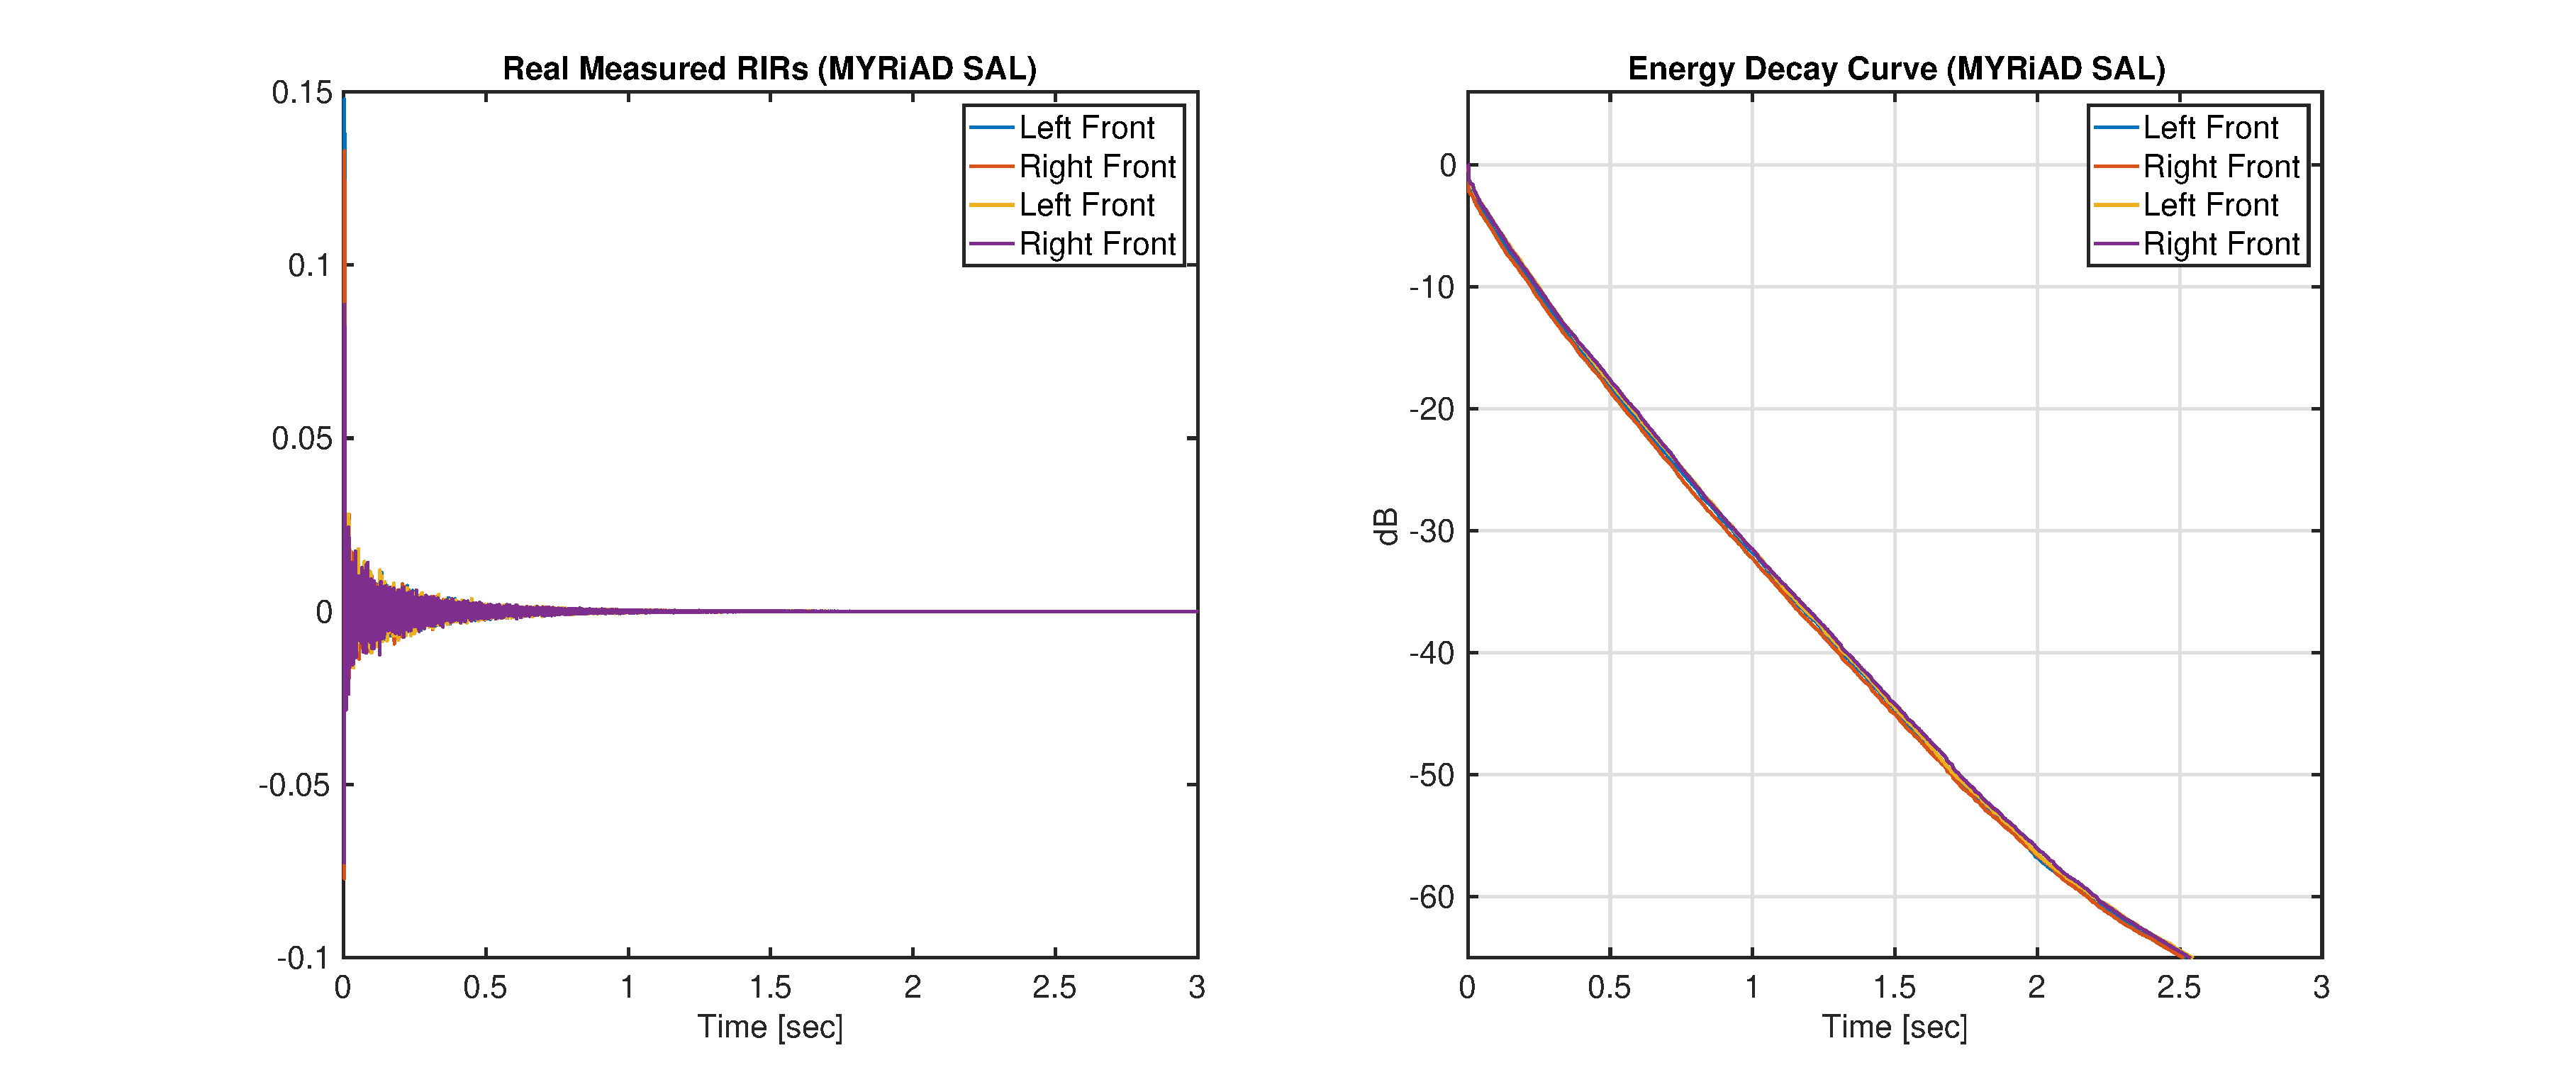
\includegraphics[width=1\textwidth]{RIR_EDC_SAL}
	\centering
	\caption{EIR and EDC of the MYRiAD database SAL room}
	\label{fig:RIR_EDC_SAL}
\end{figure}

% - Listed as 2.1 sec (2100 msec) in paper
% - Measured as approx:
% 		--> T60 = 2200 msec
%		--> T30 = 2*(1159-100) = 2118 msec

As expected, the EDCs all were found to decay approximately exponentially (linearly in \unit{\decibel}) during the late decay region, and have more distinct steps during the early decay region. All the RIRs from the HRIR database fall off rapidly around the \qty{400}{\milli\sec} mark due to windowing applied during the IR measurement process. This windowing was applied because measurements were collected in the presence of ambient noise and therefore the later part of the RIRs was close to the noise floor.

Table \ref{table:rir_reverb_times} summarizes the reverberation times  specified in the original papers for each database and various reverberation metrics measured from the EDCs shown above.

\begin{table}[H]
	\begin{tabular}{ |p{0.19\textwidth}||p{0.15\textwidth}|p{0.15\textwidth}|p{0.15\textwidth}|p{0.15\textwidth}|  }
		\hline
		 & HRIR \newline Office & HRIR \newline Courtyard & HRIR \newline Cafeteria & MYRiAD \newline SAL \\
		\hline
		\hline
		 Cited \newline Reverberation Time  & 
		 T60 =\newline \qty{300}{\milli\sec}  & 
		 T60 =\newline \qty{900}{\milli\sec} &  
		 T60 =\newline \qty{1250}{\milli\sec} & 
		 T20 =\newline \qty{2100}{\milli\sec} \\	 
		 \hline
		 Measured T60  & 
		T60 =\newline \qty{413}{\milli\sec}  & 
		T60 =\newline \qty{426}{\milli\sec} &  
		T60 =\newline \qty{437}{\milli\sec} & 
		T60 =\newline \qty{2200}{\milli\sec} \\	 
		\hline
		Measured T30  & 
		T30 =\newline \qty{400}{\milli\sec}  & 
		T30 =\newline \qty{390}{\milli\sec} &  
		T30 =\newline \qty{542}{\milli\sec} & 
		T30 =\newline \qty{2118}{\milli\sec} \\	 
		\hline
		Measured EDT  & 
		EDT =\newline \qty{4}{\milli\sec}  & 
		EDT =\newline \qty{8}{\milli\sec} &  
		EDT =\newline \qty{2}{\milli\sec} & 
		EDT =\newline \qty{230}{\milli\sec} \\	 
		\hline
		Measured C50  & 
		C50 =\newline \qty{11.9}{\decibel}  & 
		C50 =\newline \qty{29}{\decibel}&  
		C50 =\newline \qty{20.8}{\decibel}& 
		C50 =\newline \qty{1.3}{\decibel}\\	 
		\hline
	\end{tabular}
	\caption{Reverberation times specified for RIRs in their original papers, and various reverberation metrics measured from the EDCs above.}
	\label{table:rir_reverb_times}
\end{table}

The reverberation time in the SAL room in the MYRiAD database is reported as a T20, which roughly matched the T30 that was observed from the plotted EDC in Figure \ref{fig:RIR_EDC_SAL}. The measured T60 of the SAL room also closely matched the reported T20 since the decay rate of the early decay region was similar to that of the late decay region (i.e., the SAL room is more diffuse). 

Due to the windowing applied to the RIRs from the HRIR database, the measured T60 was similar accross all rooms, and therefore T60 is not a valid metric. However, the original paper reported reverberation time as ``T60" which was computed from a linear fit of the EDC. This reverberation time definition is more similar to a T20 or T30, but is not exactly the same. The measured T30 was thus found to be quite different from the originally reported T60 as well.

The measured T30s in Table \ref{table:rir_reverb_times} will be used as ``reverberation time" for the following studies.


%Discuss:
% - Add early decay time (EDT) to  chapter 1
% - How T60s were calculated in the papers compared to true T60s I'm citing
% - EDT of each
% - Noise data available also in HRIR (and MYRiAD?)

\subsection{Evaluation of Equalization-Cancellation Front-End}

The EC algorithm was evaluated on the basis of how well it emulates the main perceptual adaptations involved in reverberation processing, namely spatial release from masking (SRM) and the perceptual SNR boost of early reflections (which is largely explained by the precedence effect). Throughout this section the perceptual benefit of EC was measured using HASPI for SI prediction.

\subsubsection{Spatial Release from Noise Masking}

As a first evaluation, the perceptual suppression of directional noise in an anechoic environment was examined. ITDs were simulated by computing the difference in time of flight between the two ears for a certain direction of arrival , assuming a inter-aural separation of \qty{15}{\centi\metre}, and applying it as a sample delay to the signals. ILDs were simulated by assuming a maximum level difference of \qty{9}{\decibel}, and linearly varying the ILD from \qty{0}{\decibel} at \qty{0}{\deg} to \qty{9}{\decibel} at \qty{90}{\deg}. This direction of arrival is defined as a clockwise rotation from the front of the head (i.e., \qty{-90}{\deg} implies sound arriving from the left side of the head). The speech source was placed at \qty{0}{\deg}, and synthetic white noise was generated as the noise source. An SNR of \qty{-12}{\decibel}, which is below the speech recognition threshold (i.e., SRT as described in Section \ref{section:reverb_si}) was selected so that the noise would significantly impact intelligibility. HASPI was plotted against noise direction for each ear without EC and for the EC output (Figure \ref{fig:EC_SRM_NoiseDir}).

\begin{figure}[H]
	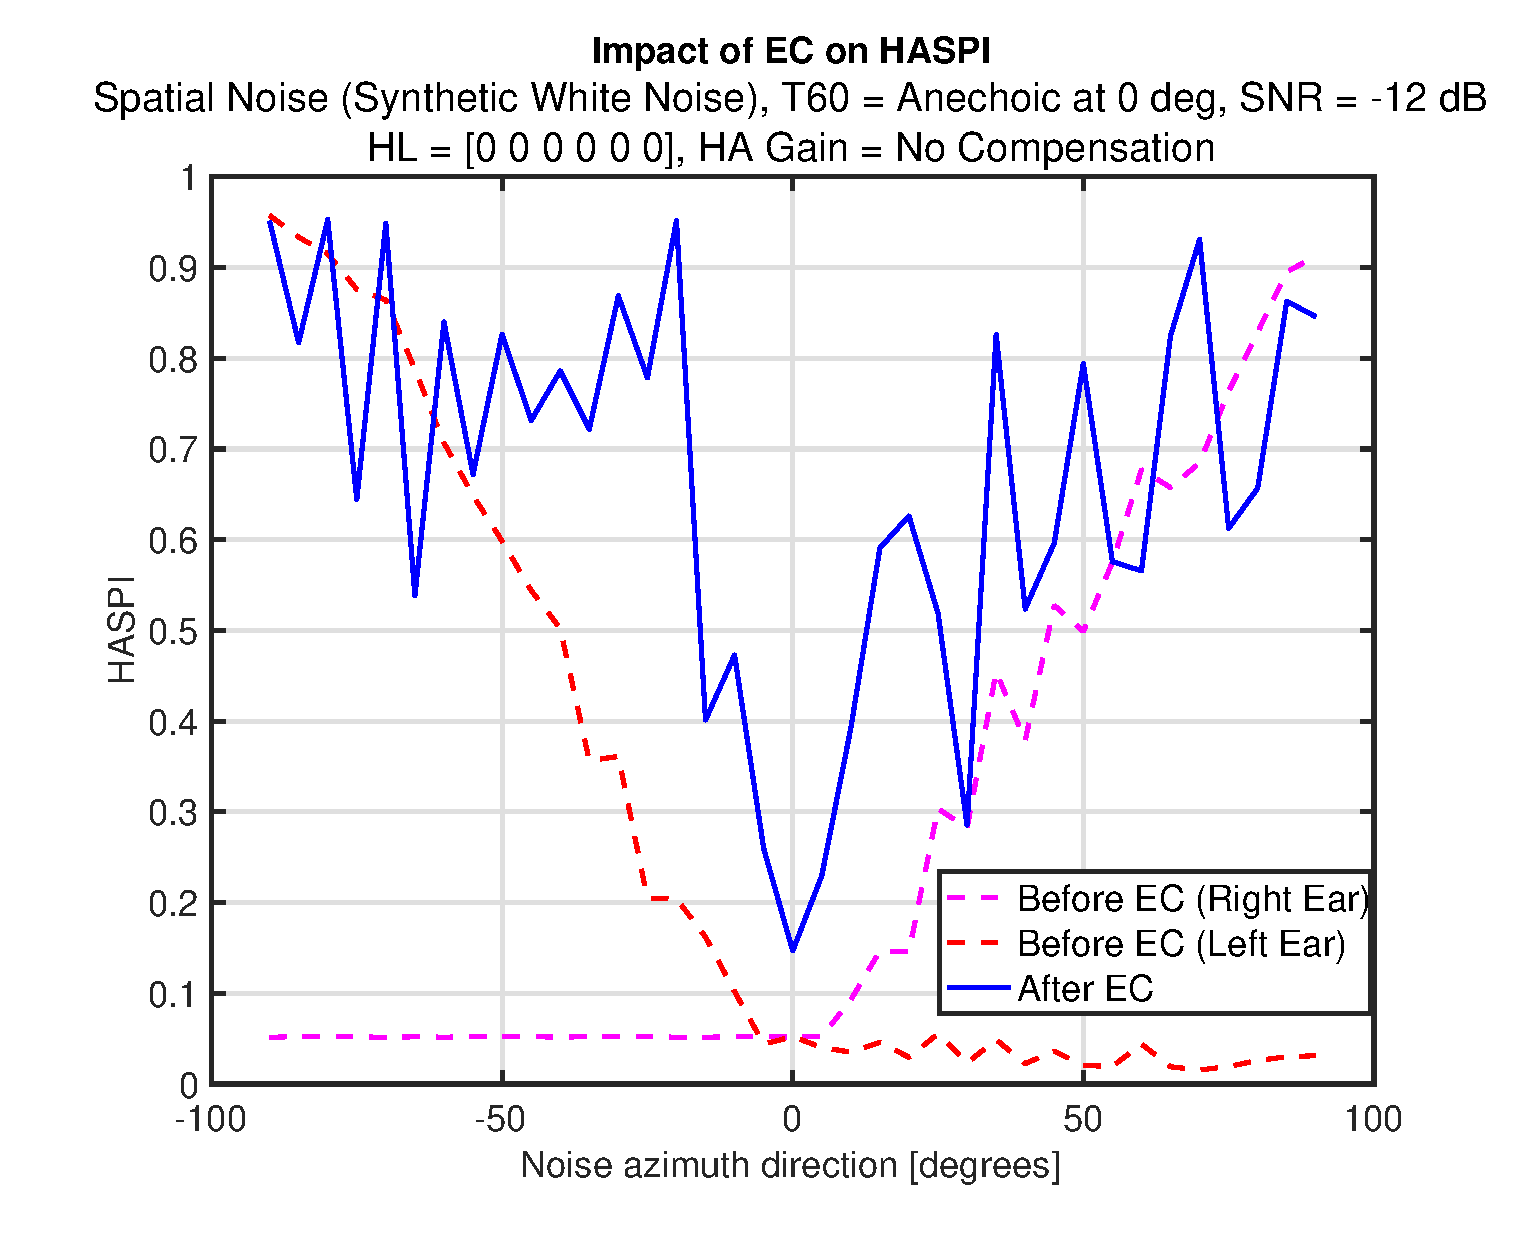
\includegraphics[width=0.7\textwidth]{EC_SRM_NoiseDir}
	\centering
	\caption[EC spatial release from masking performance for various noise direction-of-arrival]{Impact of EC algorithm on speech intelligibility (using HASPI) as a function of noise direction, anechoic directional speech and noise.}
	\label{fig:EC_SRM_NoiseDir}
\end{figure}

Without the EC front-end, a strong impact of the interfering noise on intelligibility was observed. For each ear, the simulated ILDs vary SNR from \qty{-12}{\decibel} when the noise on the corresponding side of the head, to \qty{-3}{\decibel} when it is on the other side of the head. Since these two SNRs are below and above the SRT respectively, this results in predicted SI varying from $< \qty{50}{\percent}$ to approximately \qty{100}{\percent}.

The EC front-end was observed to provide a substantial perceptual benefit, except when the direction was co-located with the speech source (i.e., at \qty{0}{\deg}). Since co-located speech and noise have the same ILDs and ITDs, the EC algorithm has limited spatial diversity cues to leverage, which aligns real perception.

Next, the perceptual release from noise masking of EC was investigated in the presence of reverberation. Synthetic white noise was generated and HASPI was plotted against SNR from \qty{-12}{\decibel} to \qty{12}{\decibel}, with and without EC. Reverberation was applied using the SAL room from the MYRiAD database with a T60 of \qty{2.1}{\sec}. The \qty{0}{\deg} location RIR from the database was used for the speech signal, and the \qty{90}{\deg} location was used for the noise signal (i.e., they were not co-located). A more exhaustive set of similar tests including diffuse speech generated with synthetic gaussian random RIRs and including spatial noise recordings and synthetic diffuse noise can be found in Appendix \ref{section:appendix:EC_eval}

\begin{figure}[H]
	\centering
	\begin{subfigure}[b]{0.49\textwidth}
		\centering
		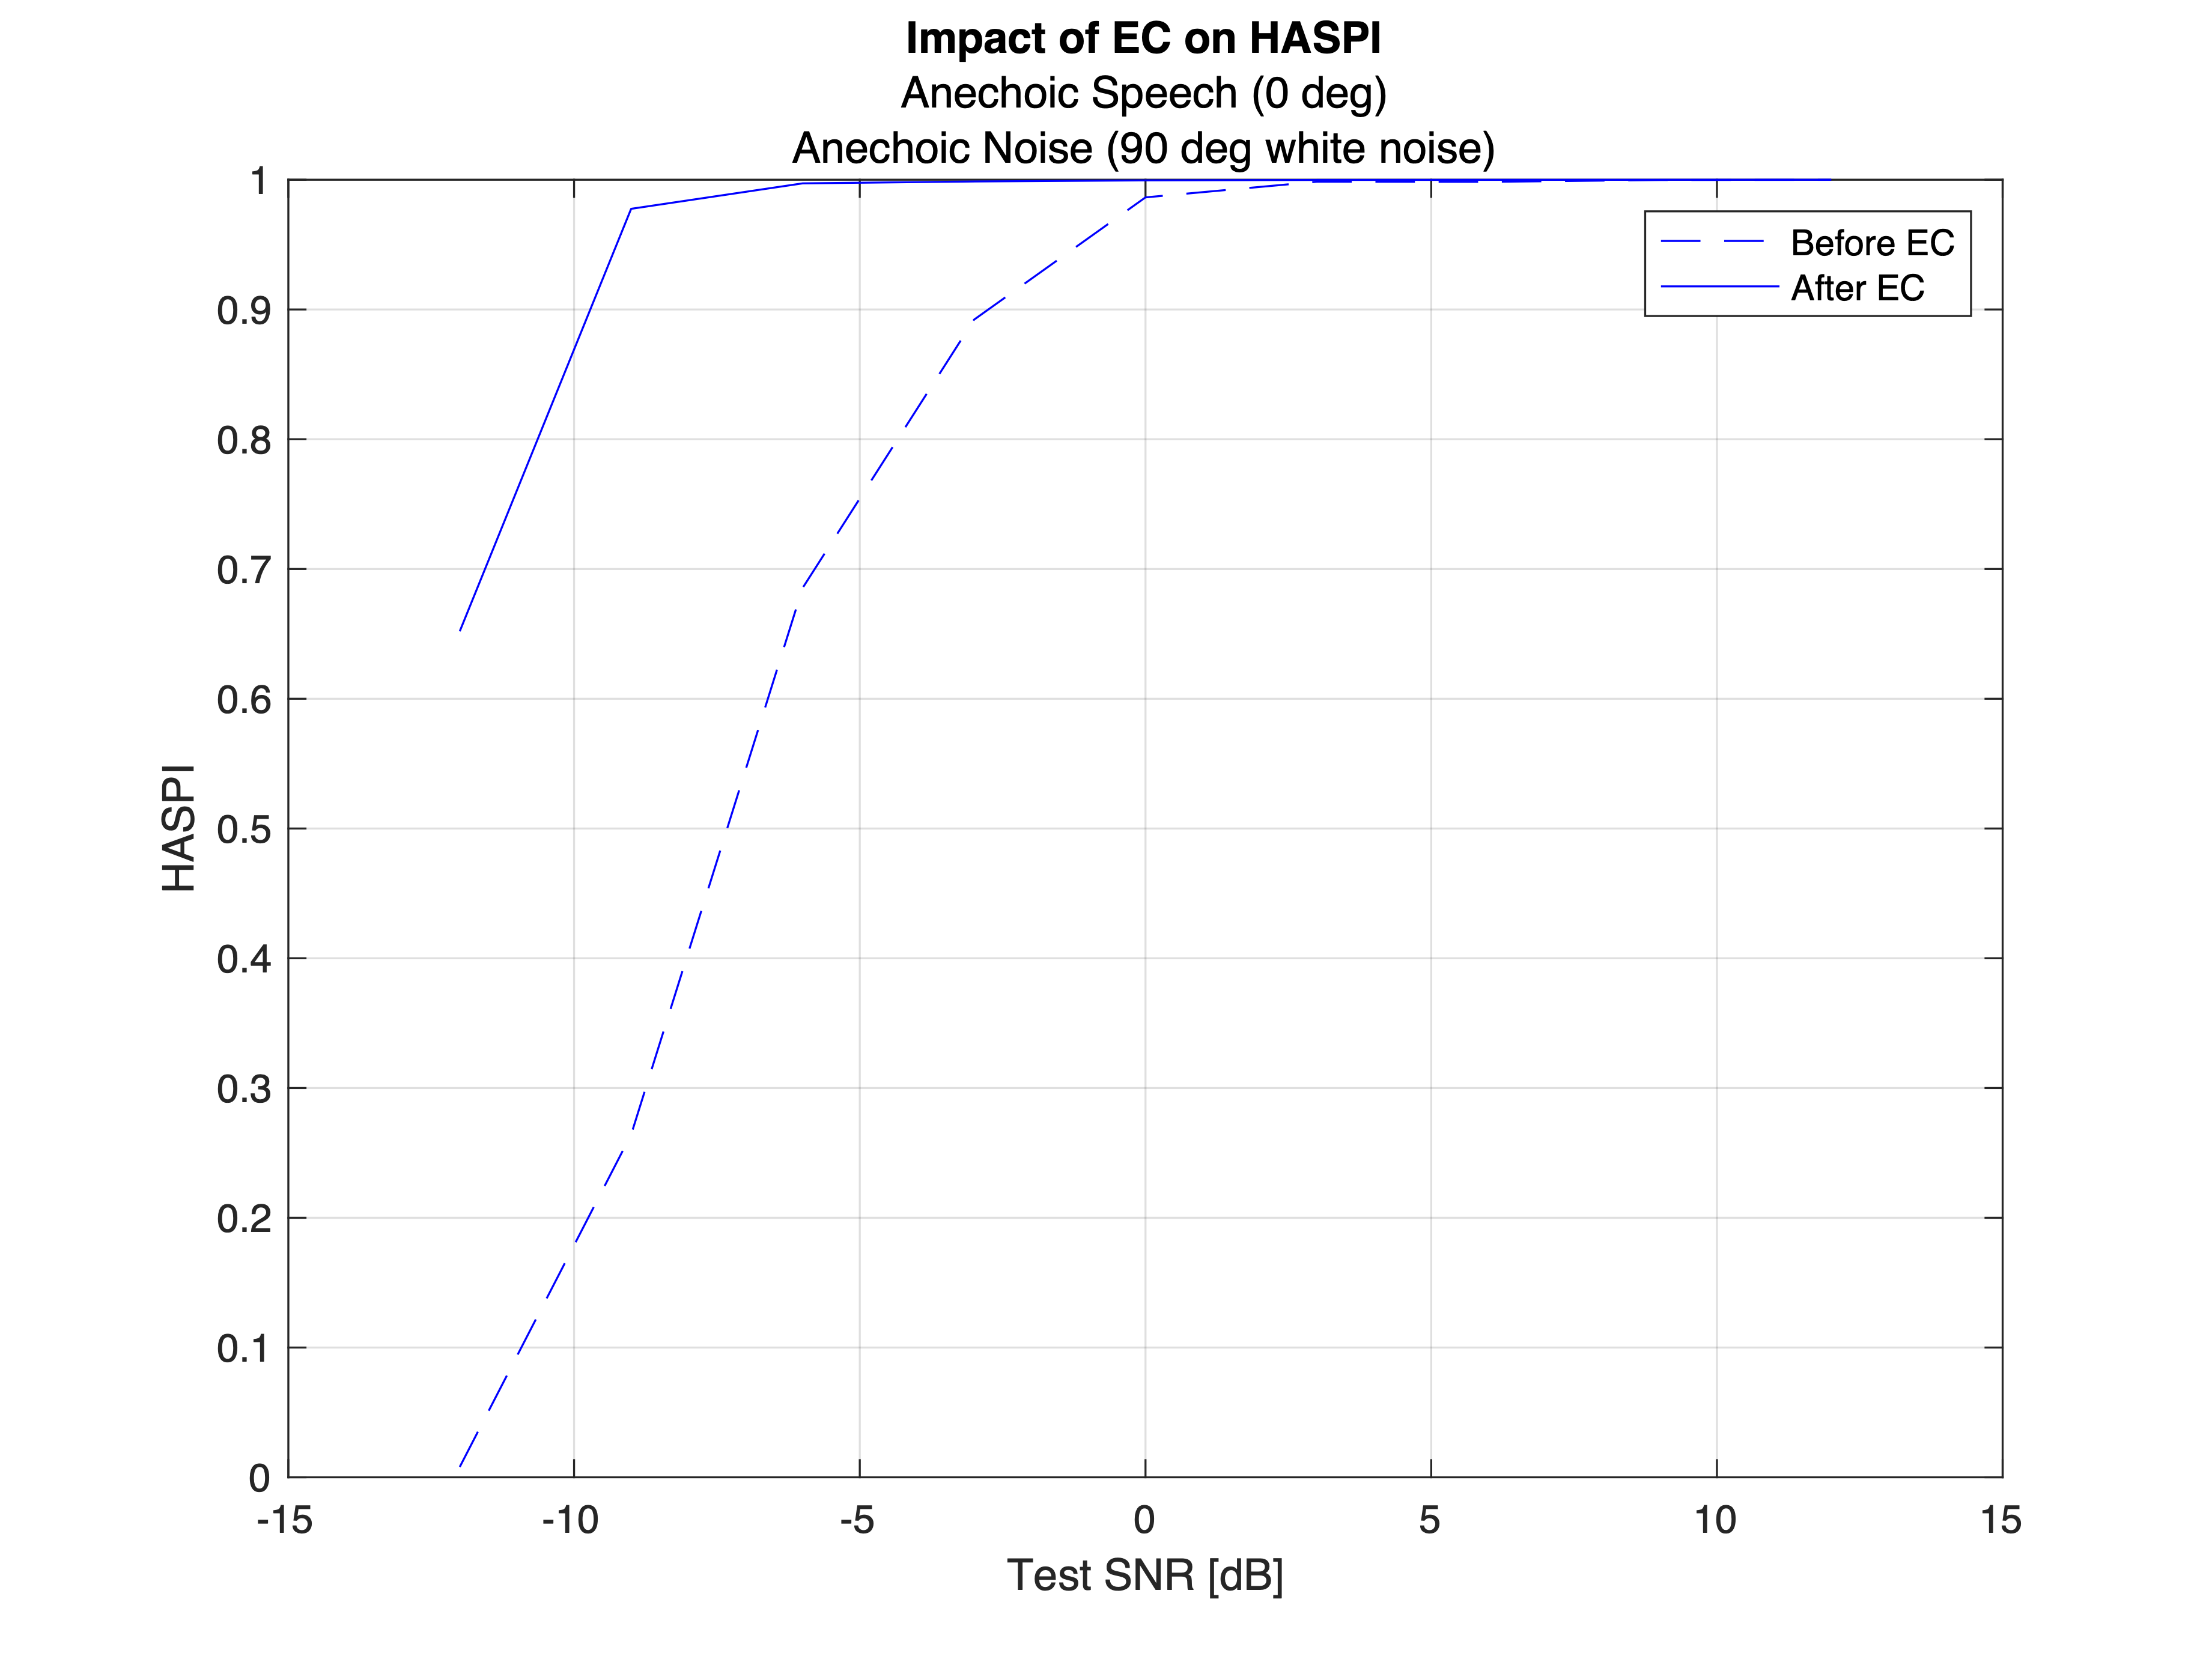
\includegraphics[width=\textwidth]{EC_SRM_AnechoicSpeech_AnechoicNoise}
		\subcaption{Anechoic Speech, Anechoic Noise}
		\label{subfig:EC_SRM_SNR_anechoicS_anechoicN}
	\end{subfigure}
	\hfill
	\begin{subfigure}[b]{0.49\textwidth}
		\centering
		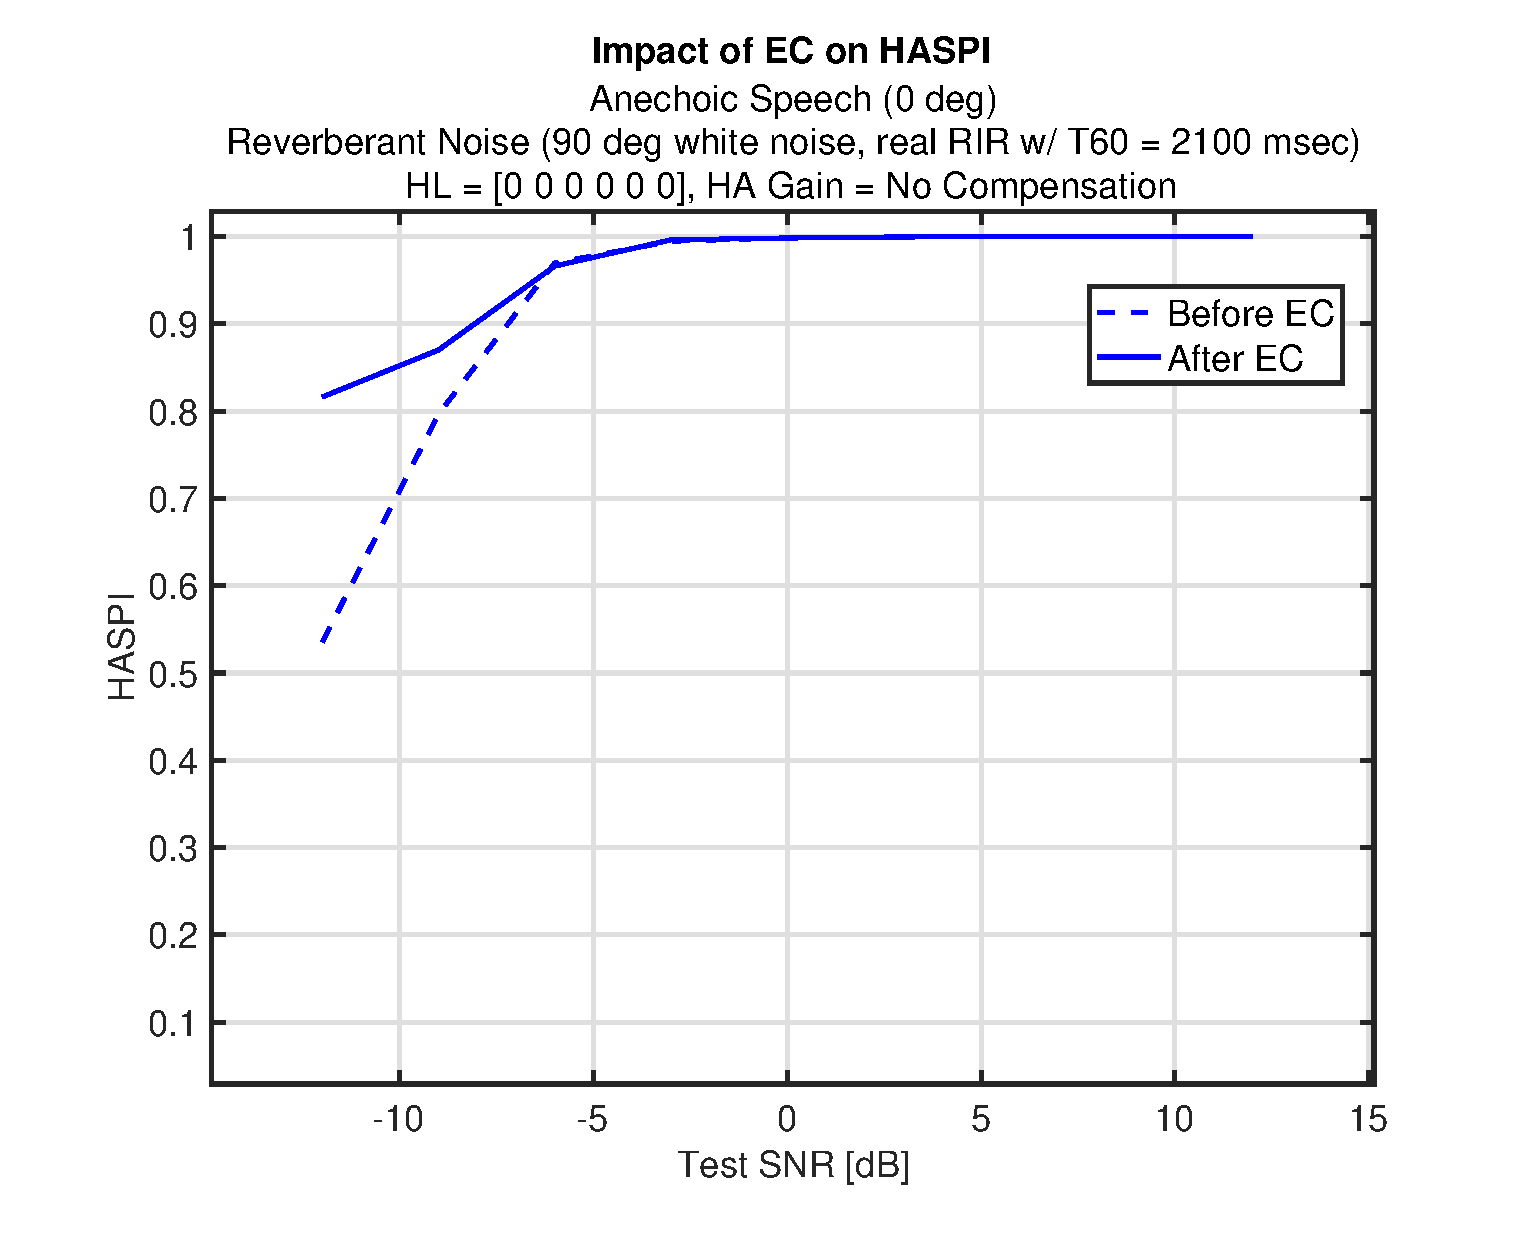
\includegraphics[width=\textwidth]{EC_SRM_AnechoicSpeech_ReverbNoise}
		\subcaption{Anechoic Speech, Reverberant Noise}
		\label{subfig:EC_SRM_SNR_anechoicS_reverbN}
	\end{subfigure}
	\hfill
	\begin{subfigure}[b]{0.49\textwidth}
		\centering
		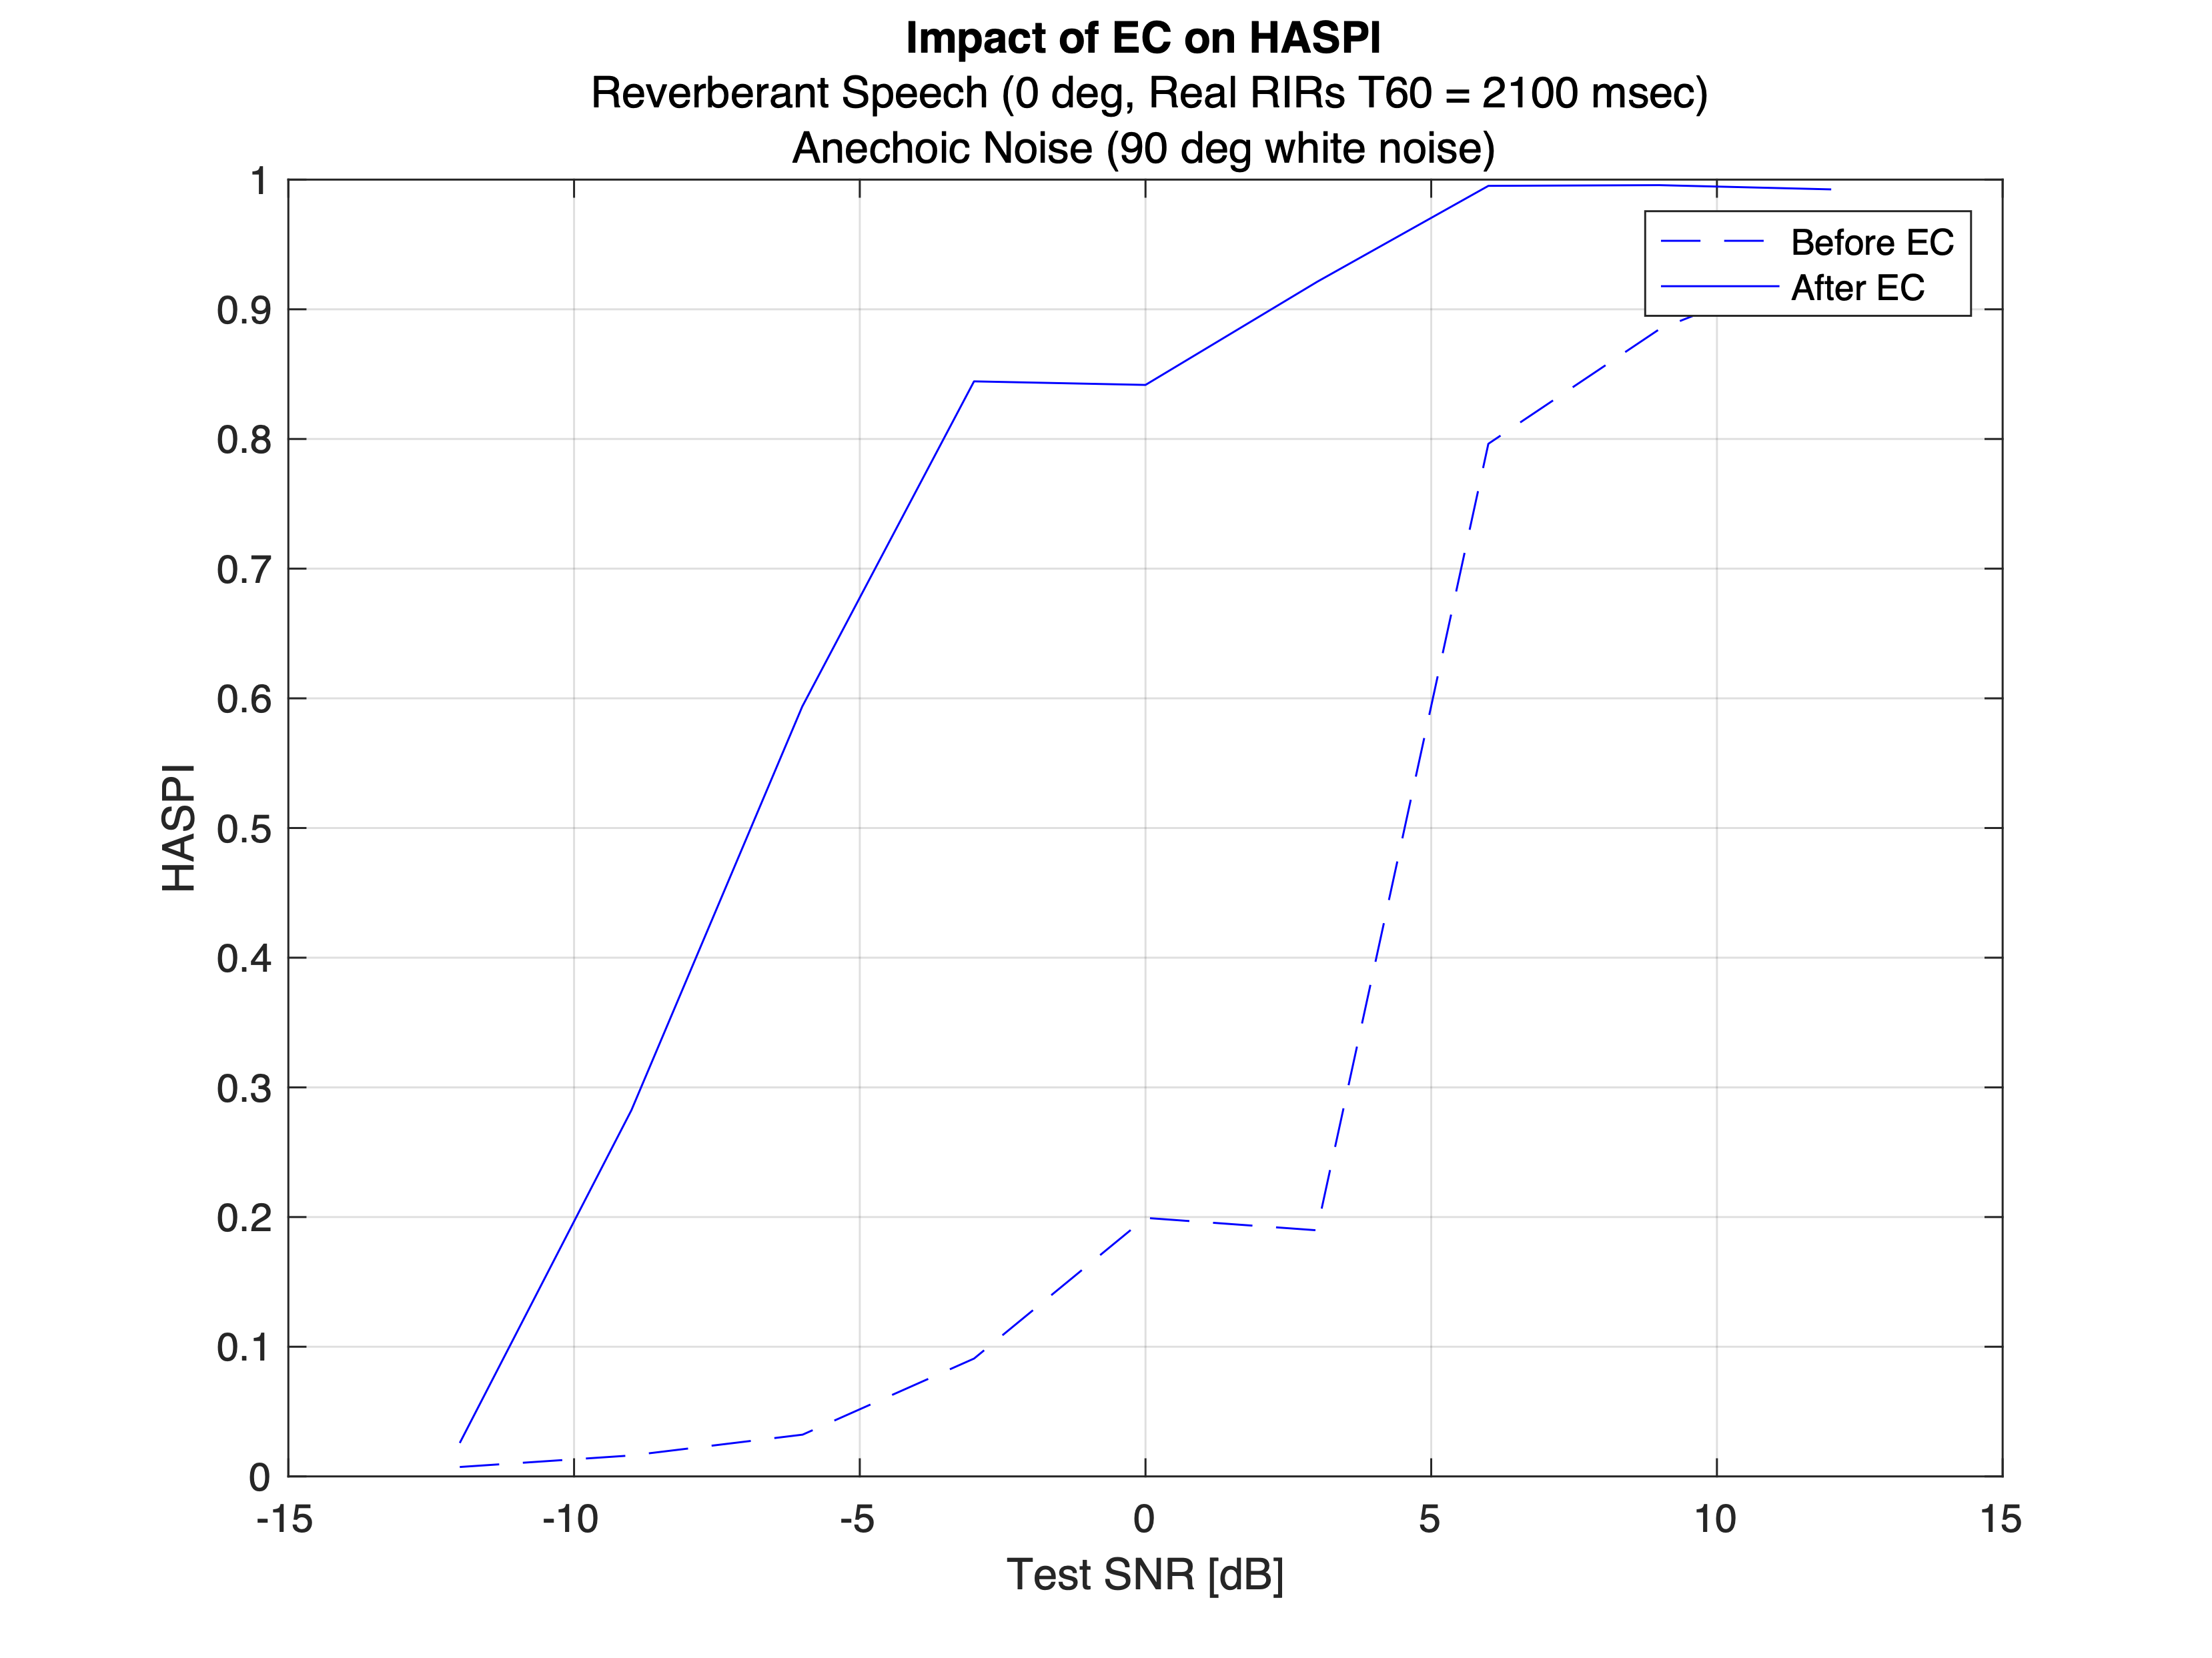
\includegraphics[width=\textwidth]{EC_SRM_ReverbSpeech_AnechoicNoise}
		\subcaption{Reverberant Speech, Anechoic Noise}
		\label{subfig:EC_SRM_SNR_reverbS_anechoicN}
	\end{subfigure}
	\hfill
	\begin{subfigure}[b]{0.49\textwidth}
		\centering
		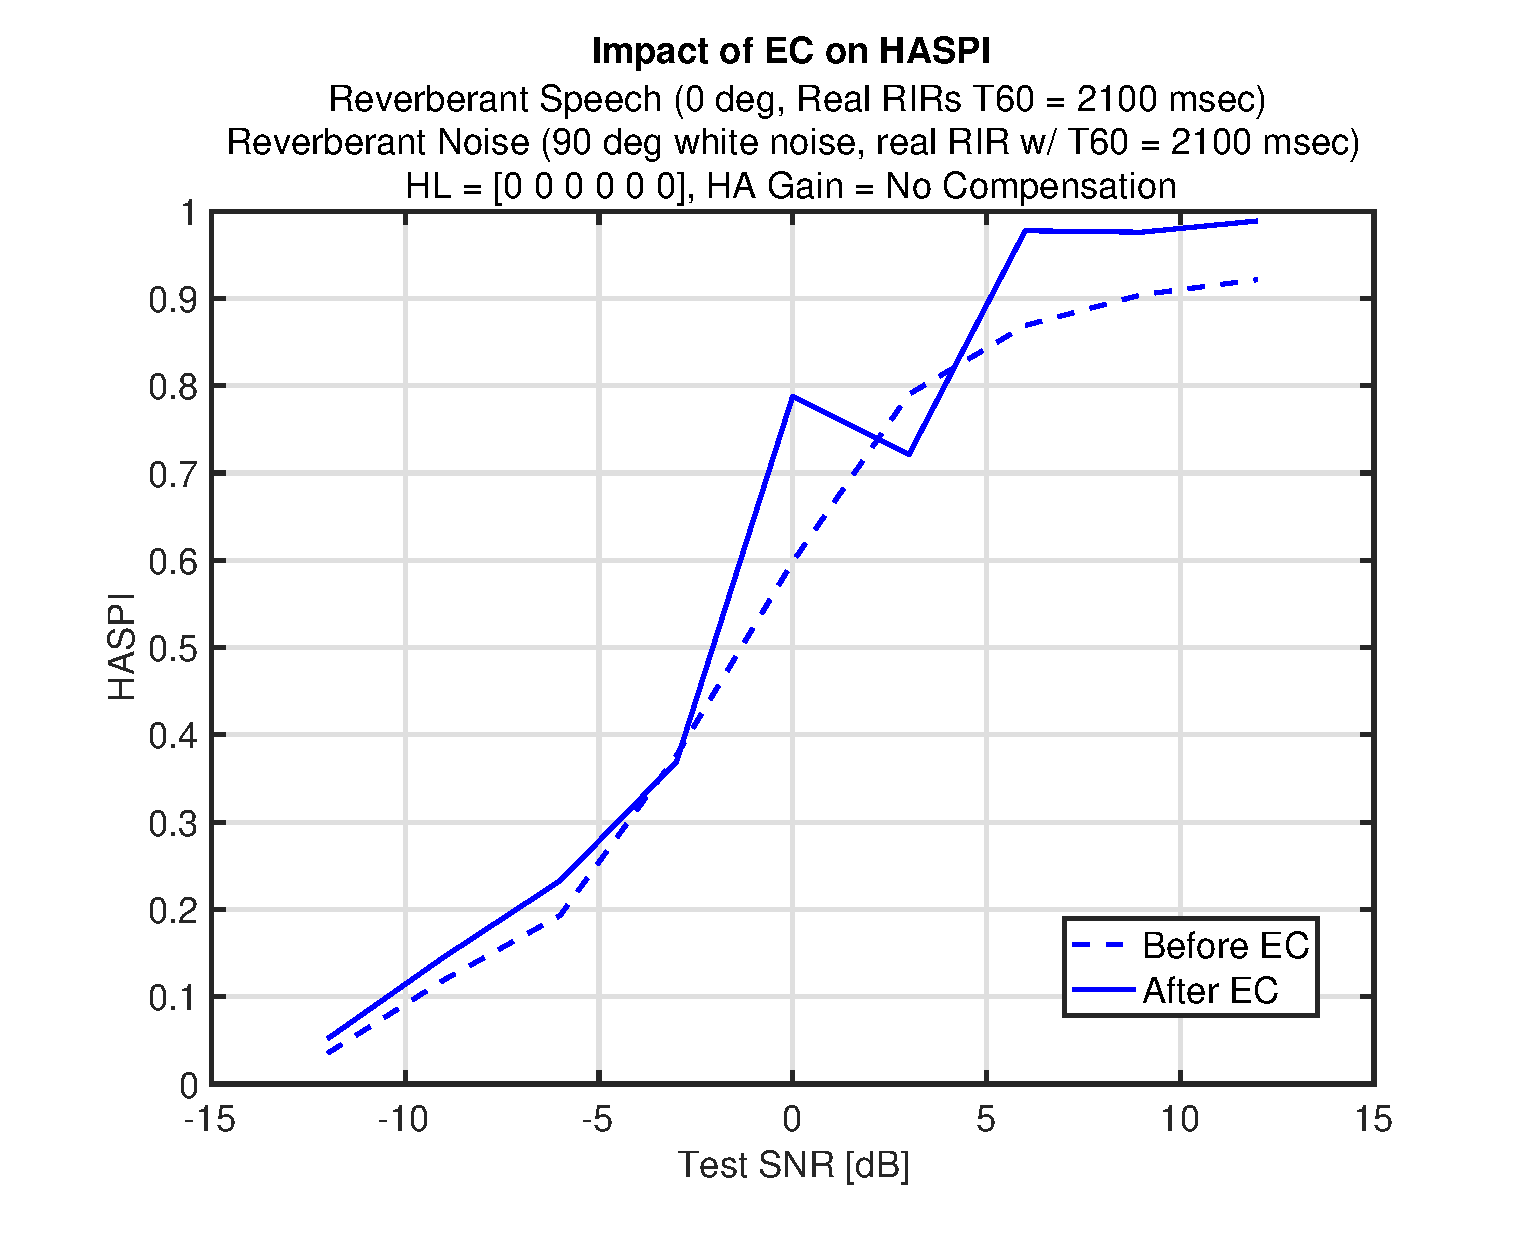
\includegraphics[width=\textwidth]{EC_SRM_ReverbSpeech_ReverbNoise}
		\subcaption{Reverberant Speech, Reverberant Noise}
		\label{subfig:EC_SRM_SNR_reverbS_reverbN}
	\end{subfigure}
	\hfill
	\caption[Impact of reverberation on EC spatial release from masking]{Impact of EC algorithm on speech intelligibility (using HASPI) as a function of SNR, for non co-located speech and white noise}
	\label{fig:EC_SRM_SNR}
\end{figure}

Significant release from noise masking was observed for anechoic noise in both the anechoic and reverberant speech cases (Figures \ref{subfig:EC_SRM_SNR_anechoicS_anechoicN} and \ref{subfig:EC_SRM_SNR_reverbS_anechoicN}). However, when the noise was reverberant (Figures \ref{subfig:EC_SRM_SNR_anechoicS_reverbN} and \ref{subfig:EC_SRM_SNR_reverbS_reverbN}), the EC provides very little benefit. This demonstrates a dependency of the EC performance on the interfering signal being focused to a particular spatial direction. This behavior holds perceptual validty as it reflects the reduction in SRM in reverberation due to distortion of spatial cues as described in Section \ref{section_srm}.

\subsubsection{Spatial Release from Reverberation Masking}

As previously discussed, SRM also provides some preceptual suppression of reverberation be attenuating the directions corresponding to reflections. To assess this behavior in the EC front-end, intelligibility was evaluated over a range of T60s in the absense of noise. In this evaluation, the RIRs were synthetically generated exponentially decaying Gaussians. The experiment was also repeated with the leading sample of the synthetic RIRs (i.e., the direct sound) increased by \qty{12}{\decibel} to make the reverberation less diffuse. The results are shown in Figure \ref{fig:EC_SRM_T60_Synth2}.

%\begin{figure}[H]
%	\centering
%	\begin{subfigure}[b]{0.49\textwidth}
%		\centering
%		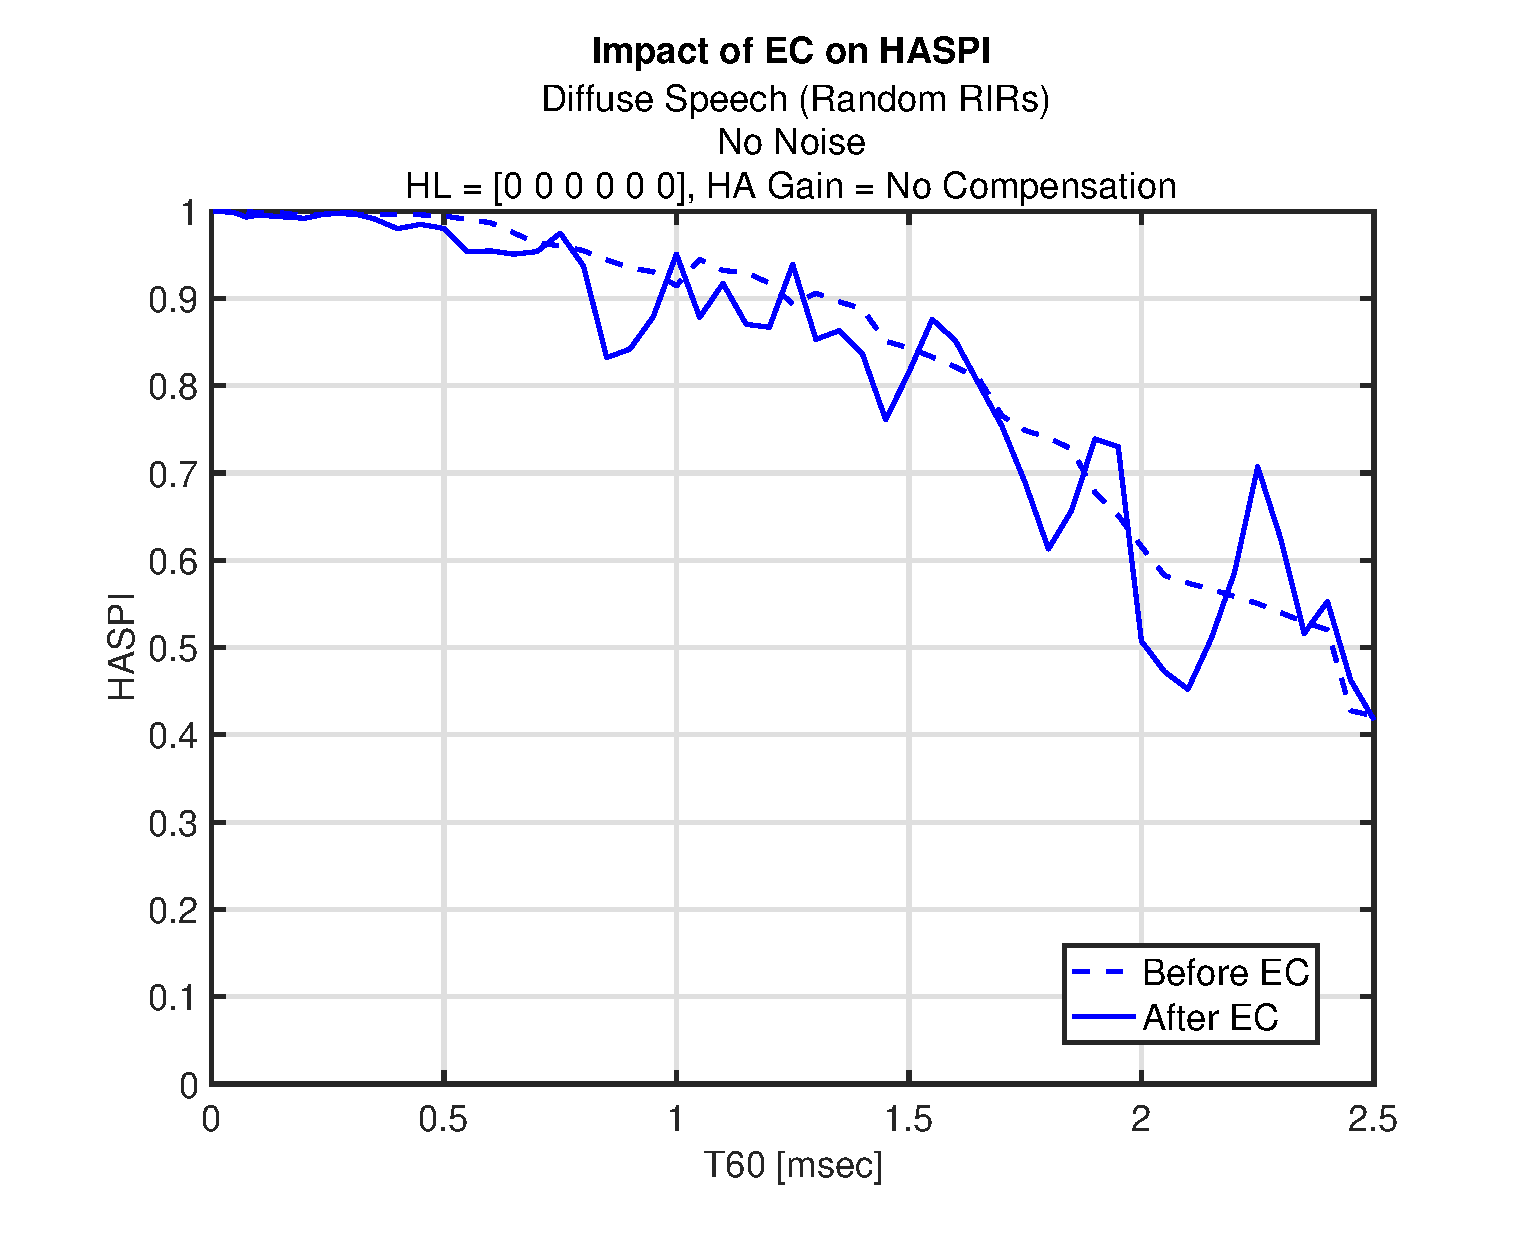
\includegraphics[width=\textwidth]{EC_SRM_T60_Synth_NoNoise}
%		\subcaption{Direct sound level = reflection level}
%		\label{subfig:EC_SRM_T60_Synth_NoNoise}
%	\end{subfigure}
%	\hfill
%	\begin{subfigure}[b]{0.49\textwidth}
%		\centering
%		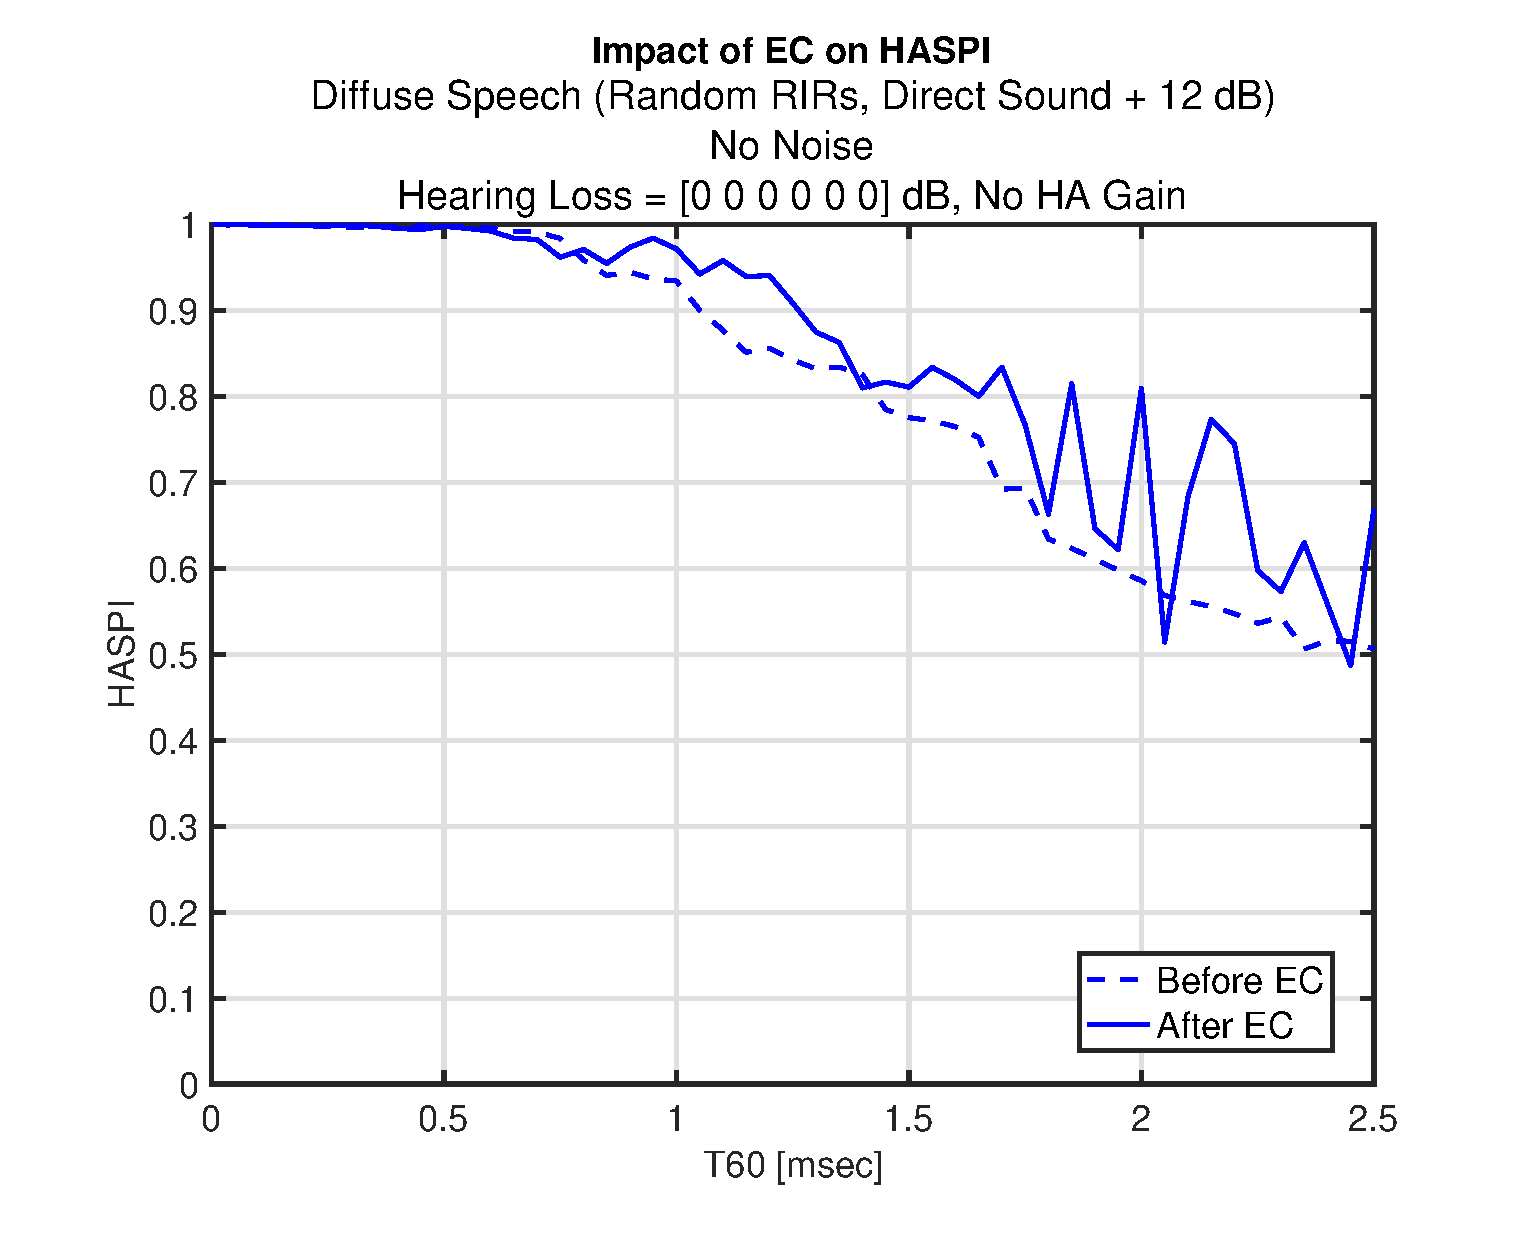
\includegraphics[width=\textwidth]{EC_SRM_T60_SynthStrongDirect_NoNoise}
%		\subcaption{Direct sound level =  reflection level + 12dB}
%		\label{subfig:EC_SRM_T60_SynthStrongDirect_NoNoise}
%	\end{subfigure}
%	\caption{\textbf{Each generated by truncation of the same random RIRs}. Impact of EC algorithm on speech intelligibility (using HASPI) as a function of varying amounts of synthetic reverb, noise-free}
%	\label{fig:EC_SRM_T60_Synth}
%\end{figure}

\begin{figure}[H]
	\centering
	\begin{subfigure}[b]{0.49\textwidth}
		\centering
		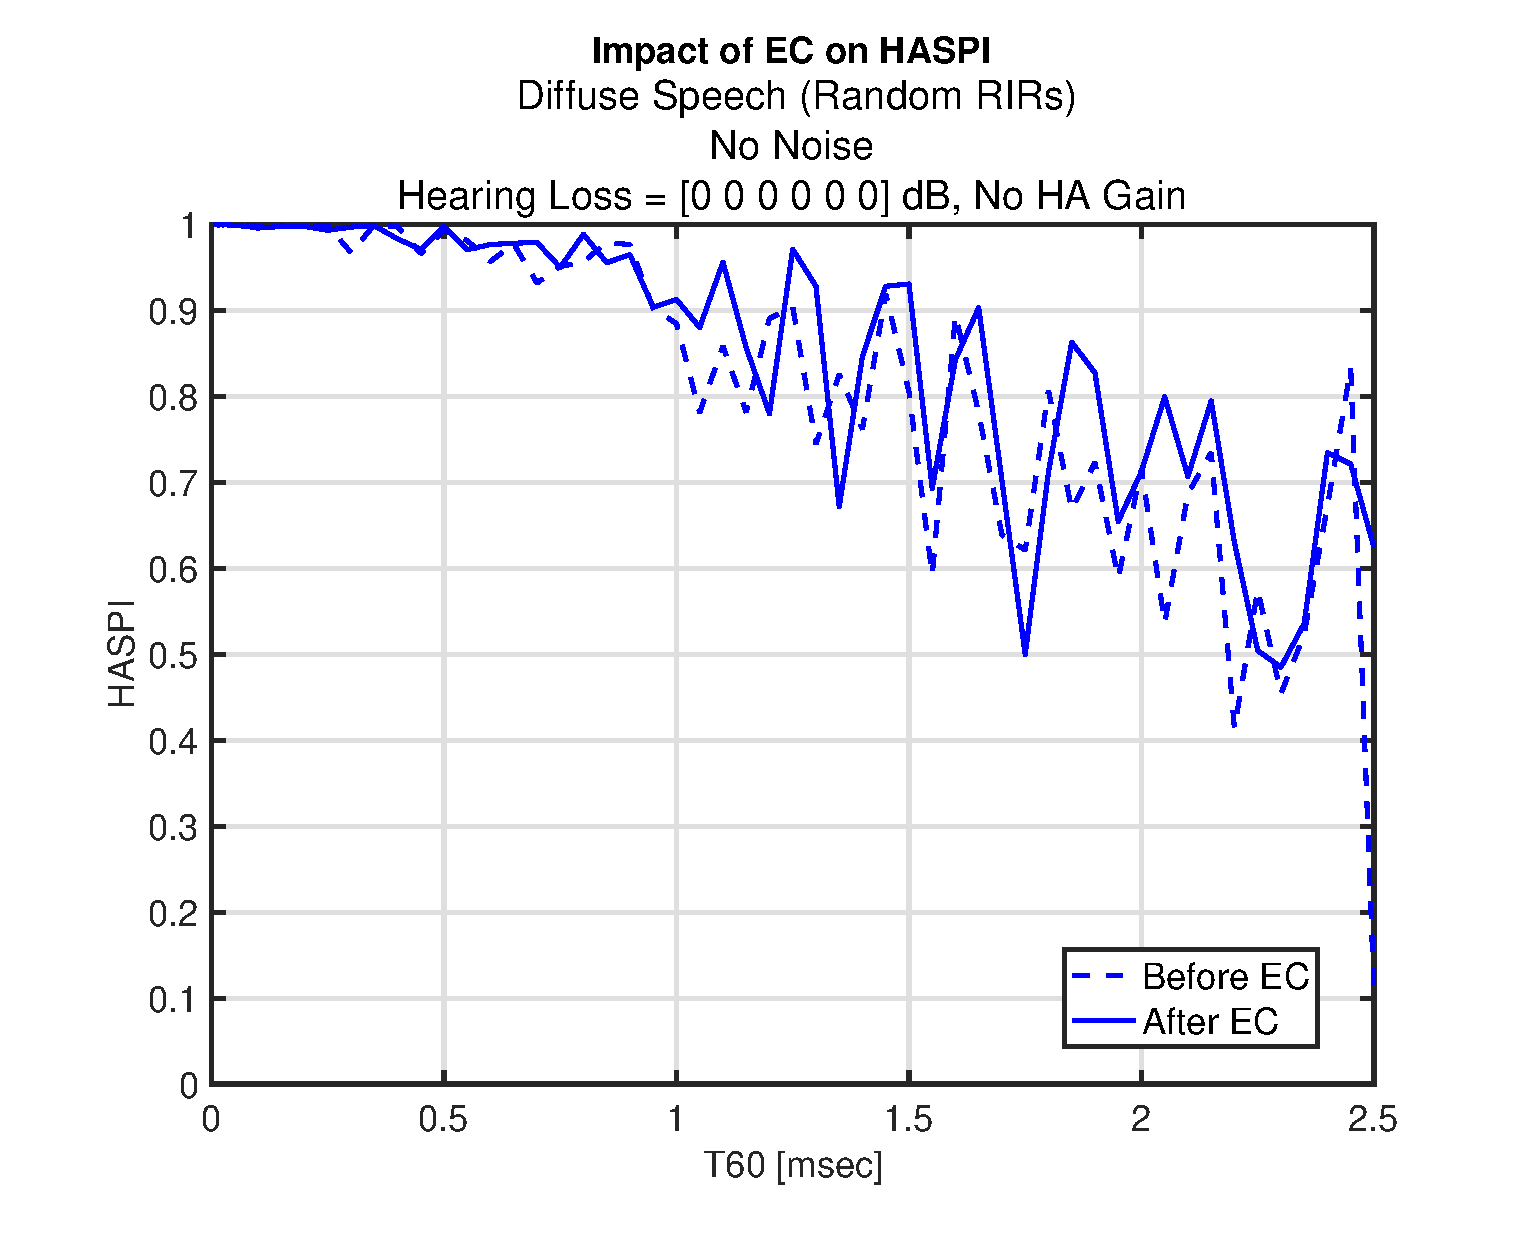
\includegraphics[width=\textwidth]{EC_SRM_T60_Synth_NoNoise_2}
		\subcaption{Direct sound level = reflection level}
		\label{subfig:EC_SRM_T60_Synth_NoNoise2}
	\end{subfigure}
	\hfill
	\begin{subfigure}[b]{0.49\textwidth}
		\centering
		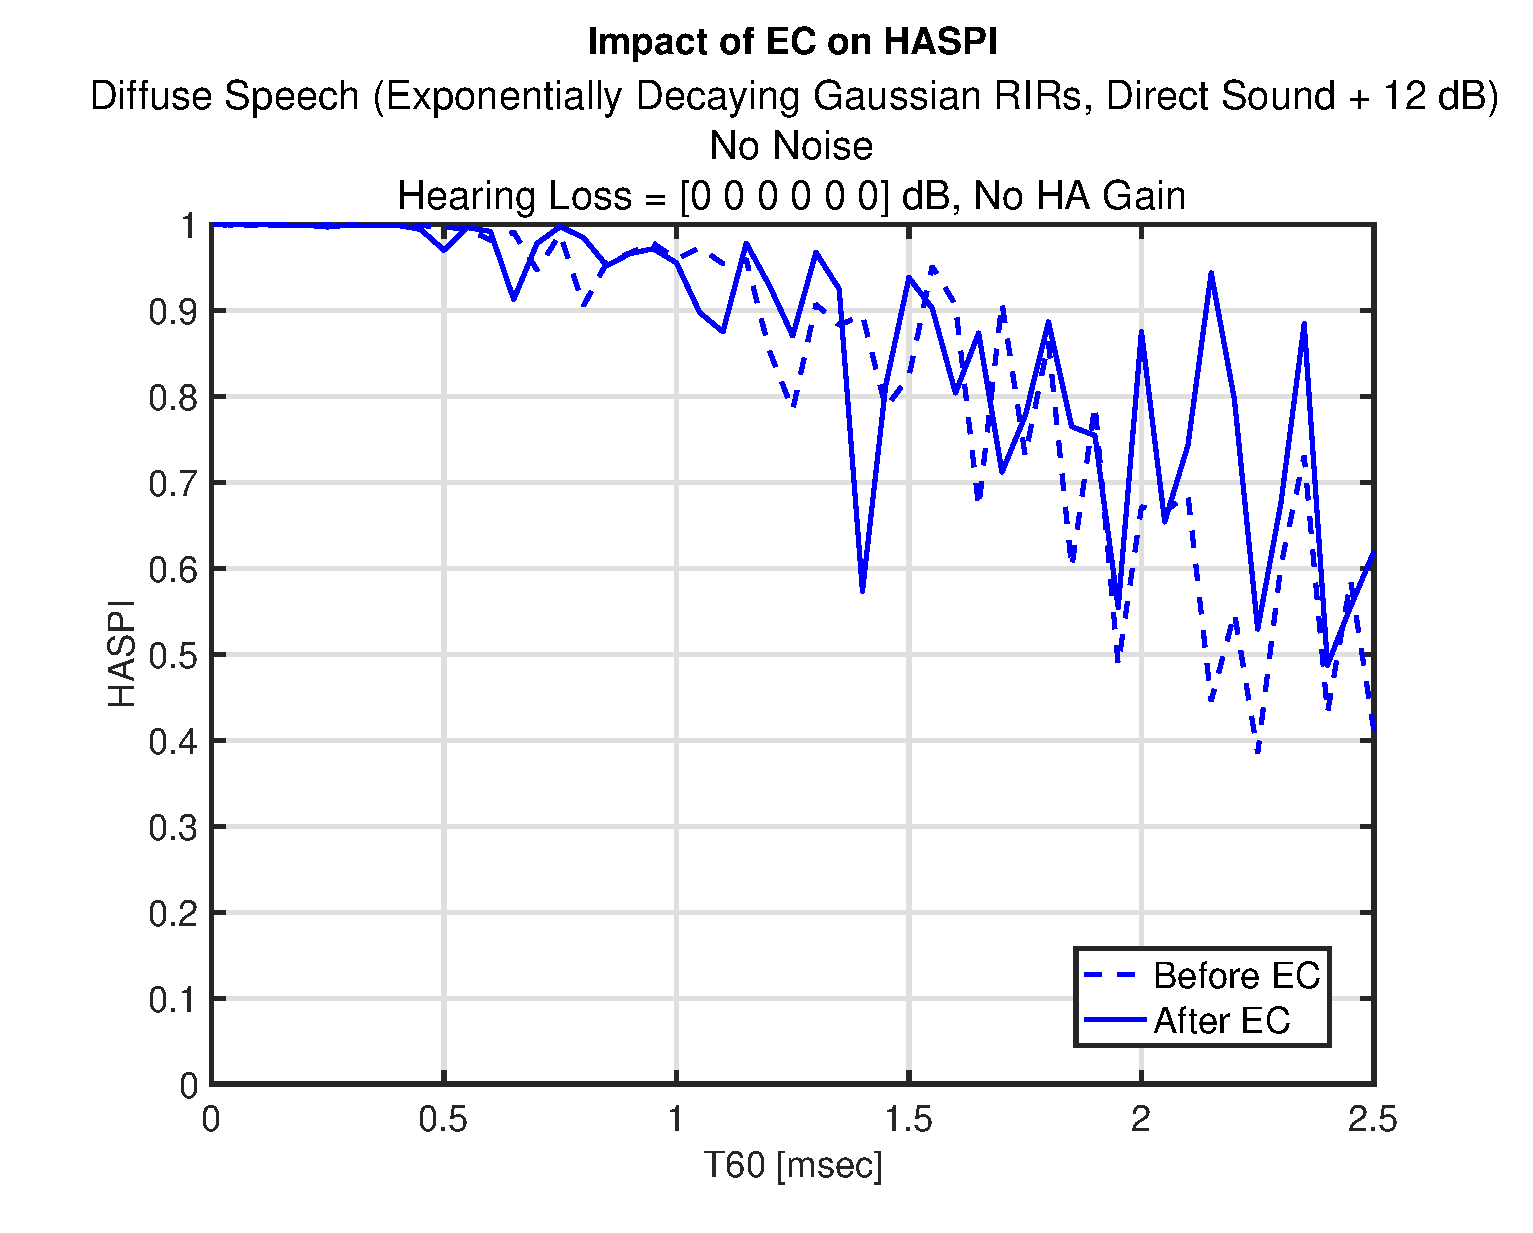
\includegraphics[width=\textwidth]{EC_SRM_T60_SynthStrongDirect_NoNoise_2}
		\subcaption{Direct sound level =  reflection level + 12dB}
		\label{subfig:EC_SRM_T60_SynthStrongDirect_NoNoise2}
	\end{subfigure}
	\caption[EC spatial release from reverberation masking performance]{Impact of EC algorithm on speech intelligibility (using HASPI) as a function of varying amounts of synthetic reverb, noise-free.}
	\label{fig:EC_SRM_T60_Synth2}
\end{figure}

In both experiments, EC was observed to have very minimal impact on intelligibility. At some T60s, the EC was actually observed to have a negative impact on intelligibility, and increasing the level of the direct sound relative to the reverberation (i.e., making it less diffuse) only resulted in a slight improvement. The limited benefit of the EC in reverberation can be explained by the fact that the EC focuses on canceling spatially isolated noise as previously discussed. It is not clear whether these limitations hold perceptual grounds. 

In general, limited information exists on the applicability of EC to reverberation since it was designed to model perceptual noise cancellation.Therefore the perceptual validity of the EC could not be validated in the context of SRM for reverberation suppression and it was decided that the EC should be left out of the evaluation and to focus on a monaural evaluation. A study using a more advanced binaural front-end was left for a future study. Not only should such a front-end be validated for perceptual validity in the context of reverberation processing, but also should account for degradation of binaural perceptual adaptations due to hearing loss.

%- EC does not provide binaural benefit in reverb

%- EC focuses on canceling interfering noise from certain directions, which doesnt apply to reducing reverb since (for high T60s) reverb tends towards diffuse, and the interfering reflections are correlated to the clean speech


%- Diffuse reverb destroys binaural cues and reduces the binaural benefit modeled by the EC (this provides modeling of the reduction in SRM due to reverb). However at low T60s the RIR is less diffuse and therefore can randomly have more emphasized directions thus sometimes providing some binaural benefit
%- Note distinction between SRM for noise and reverb (EC models reduction in SRM due to reverb, but doesnt model reduction in reverb itself)

%- SNR = 0 dB: SI is already saturated, so only evaluating impact of reverb (essentially SNR = infinity)

%\subsubsection{Benefit of Early Reflections}


%\begin{figure}[H]
%	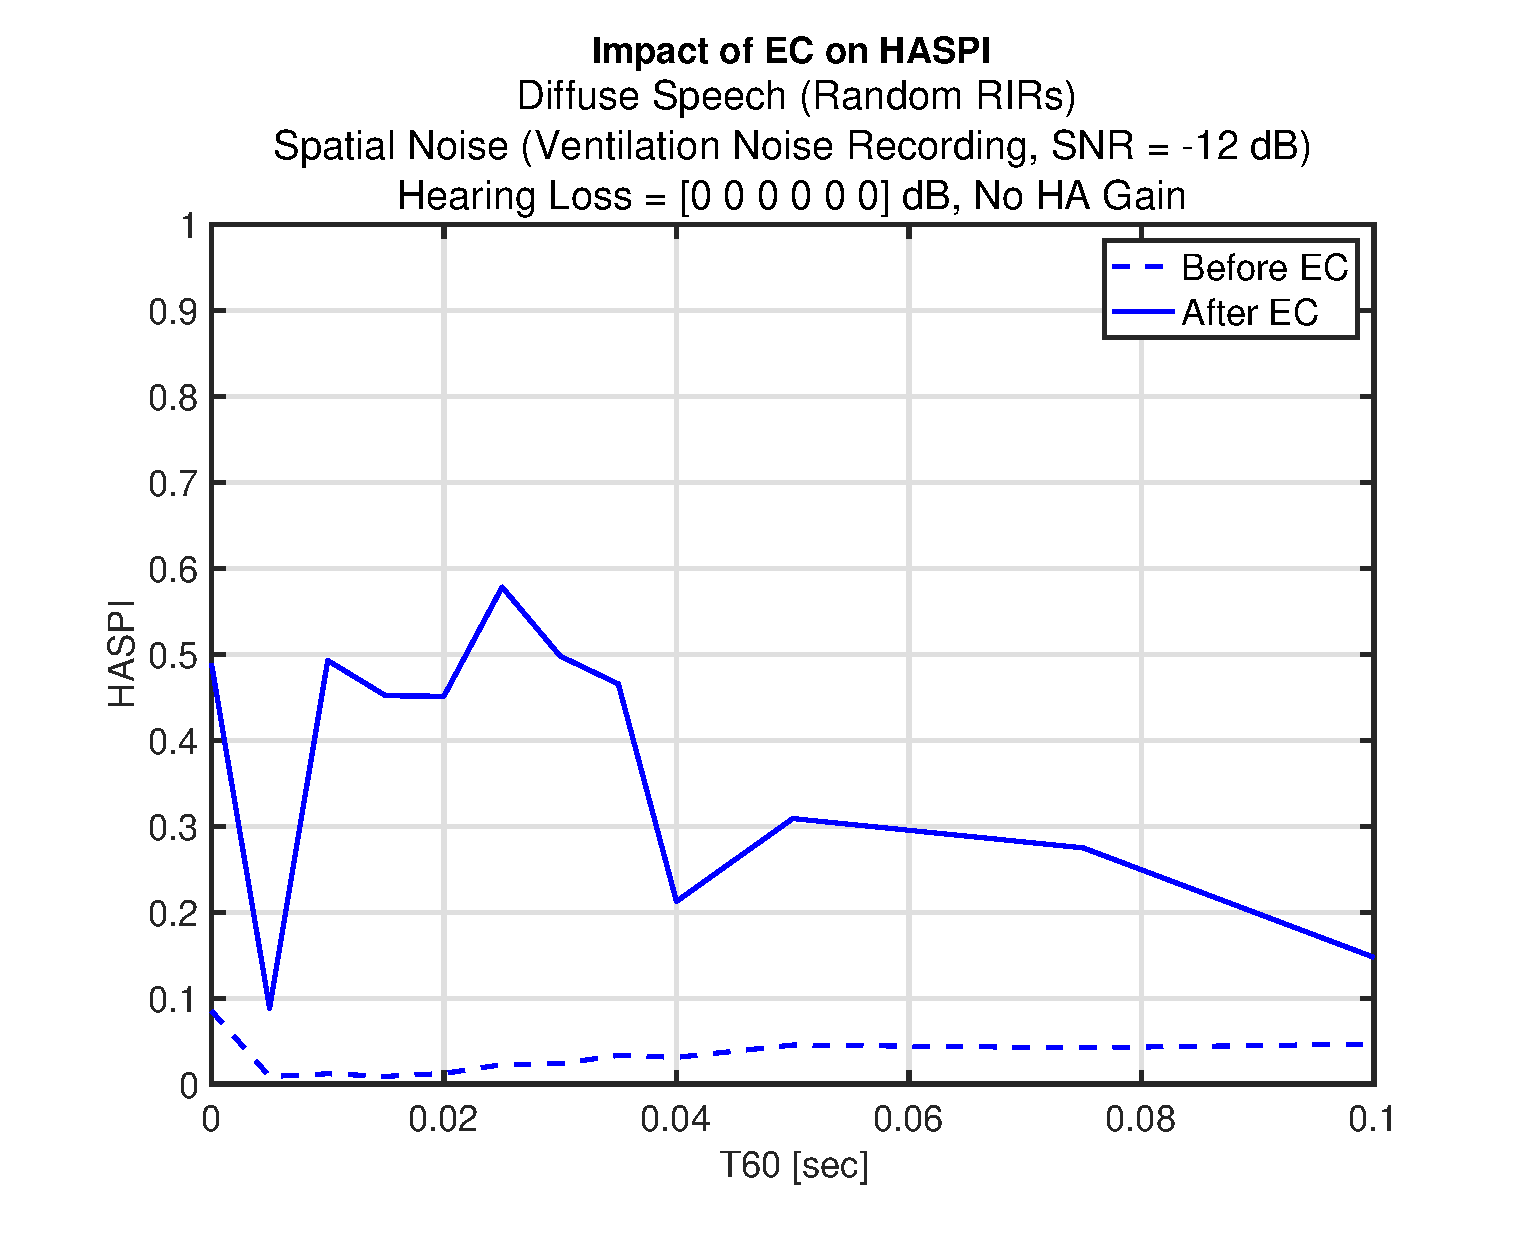
\includegraphics[width=0.7\textwidth]{EC_ERs}
%	\centering
%	\caption{Impact of EC algorithm on speech intelligibility (using HASPI) as a function of varying amounts of synthetic reverb, for spatial noise recording with SNR = \qty{-12}{\decibel}  }
%	\label{fig:EC_ReverbSNRBoost}
%\end{figure}

%- Diffuse reverb (white noise) used to focus on temporal integration rather than spatial separation -- Most significant binaural benefit for T60 = 0 (no benefit of early reflections) -- However repeating the experiment several times reveals occasional benefit depending on the randomly generated RIR -- assumed this is just due to sometimese the very short number of simulated reflections effectively coming from similar directions thus providing SRM

%- I would expect that using real RIRs would result in some SRM from early reflections (since they tend not to be diffuse)

%- Essentially all this shows that EC may provide some modeling of BINAURAL benefit of reverb in low SNR environments (SRM), but no modeling of MONAURAL benefit of reverb (PE temporal integration)


\subsection{Hearing Aid Gain Comparison} \label{sec:ha_gain_comparison}

When evaluating the impact of reverberation on speech perception (and subsequently the benefit of a dereverberation algorithm) in the context of hearing loss, it was important to include some gain to compensate the impairment. Without any gain, audibility would impact intelligibility and may obscure the impact of reverberation on speech cues. As discussed in Section \ref{section:hearing_loss_impacts}, hearing loss has a severe impact on quiet sounds but less so on louder sounds, motivating the use of wide dynamic range compression (WDRC) algorithms in hearing aids. Moreover, as discussed in Section \ref{section:encoding_acoustic_cues}, WDRC and other more sophisticated algorithms are necessary to jointly restore ENV and TFS acoustic cues.  It was not desirable to include more complex algorithms such as WDRC in this study, since the goal is to solely evaluate the impact of dereverberation, therefore a linear hearing aid gain vector had to be selected. A linear equalizer that directly compensates the specific hearing loss (i.e., audiogram mirror equalizer) is optimal for making quiet sounds audible but would make louder sounds far too loud. Additionally TFS acoustic cues are more heavily distorted by higher sound pressure levels, thus higher gains are generally beneficial for the audibility of ENV cues but have a negative impact on TFS cue perception. These tradeoffs were discussed by \cite{byrne1986national}, and a perceptually optimal linear gain known as the NAL-R (National Acoustic Laboritories Revised) fitting procedure was proposed. Note however that this research was based on clean speech in noise, and did not consider reverberation. Figure \ref{fig:HA_GainComparison} shows a comparison on the basis of intelligibility as a function of T60 of four hearing aid gains: no hearing aid gain, audiogram mirror gain, NAL-R gain, and a ``hybrid" gain which was placed halfway between the audiogram mirror and NAL-R (as shown in Figure \ref{fig:HA_Gains}). Intelligibility was evaluated using HASPI, FT-NSIM, MR-NSIM and STMI. The RIRs used were synthetic exponentially decaying Gaussians. The acoustic stimulius level was set to \qty{65}{\decibel SPL} to evaluate conversational speech, since this is what will be used for the remainer of this thesis.

%Ian:
%
%- Loudness recruitment and its influence on WDRC design (Threshold of hearing increasing doesnt increase in upper limit where loudness becomes too much -- reduced dynamic range)
%
%- Question: Do nonlinearities in auditory system still apply at same higher SPL with hearing loss? If so then this is another reason for not doing mirror audiogram compensation (not just comfort, but going to these high levels will distort cues making SI worse -- Shouldnt this be picked up by the metrics?)
%
%- Look at Hearing Aid textbook from Harvey Dillon
%
%- NAL-R ideal at conversational speech, quieter you want closer to mirror audiogram, and louder sounds you want less than NAL-R
%
%- Generally speaking in terms of restoring the representation (maybe also in STMI/NSIM -- pretty sure Ian knows but im missing something) mirror audiogram will be optimal for SI, NAL-R is more about comfort -- We cant do mirror audiogram because users wont like it, NAL-R is better in terms of trade off of SI and comfort

%\citep{bisgaard2010standard}, and NAL-R refers to the gain proposed by \cite{byrne1986national}.

\begin{figure}[H]
	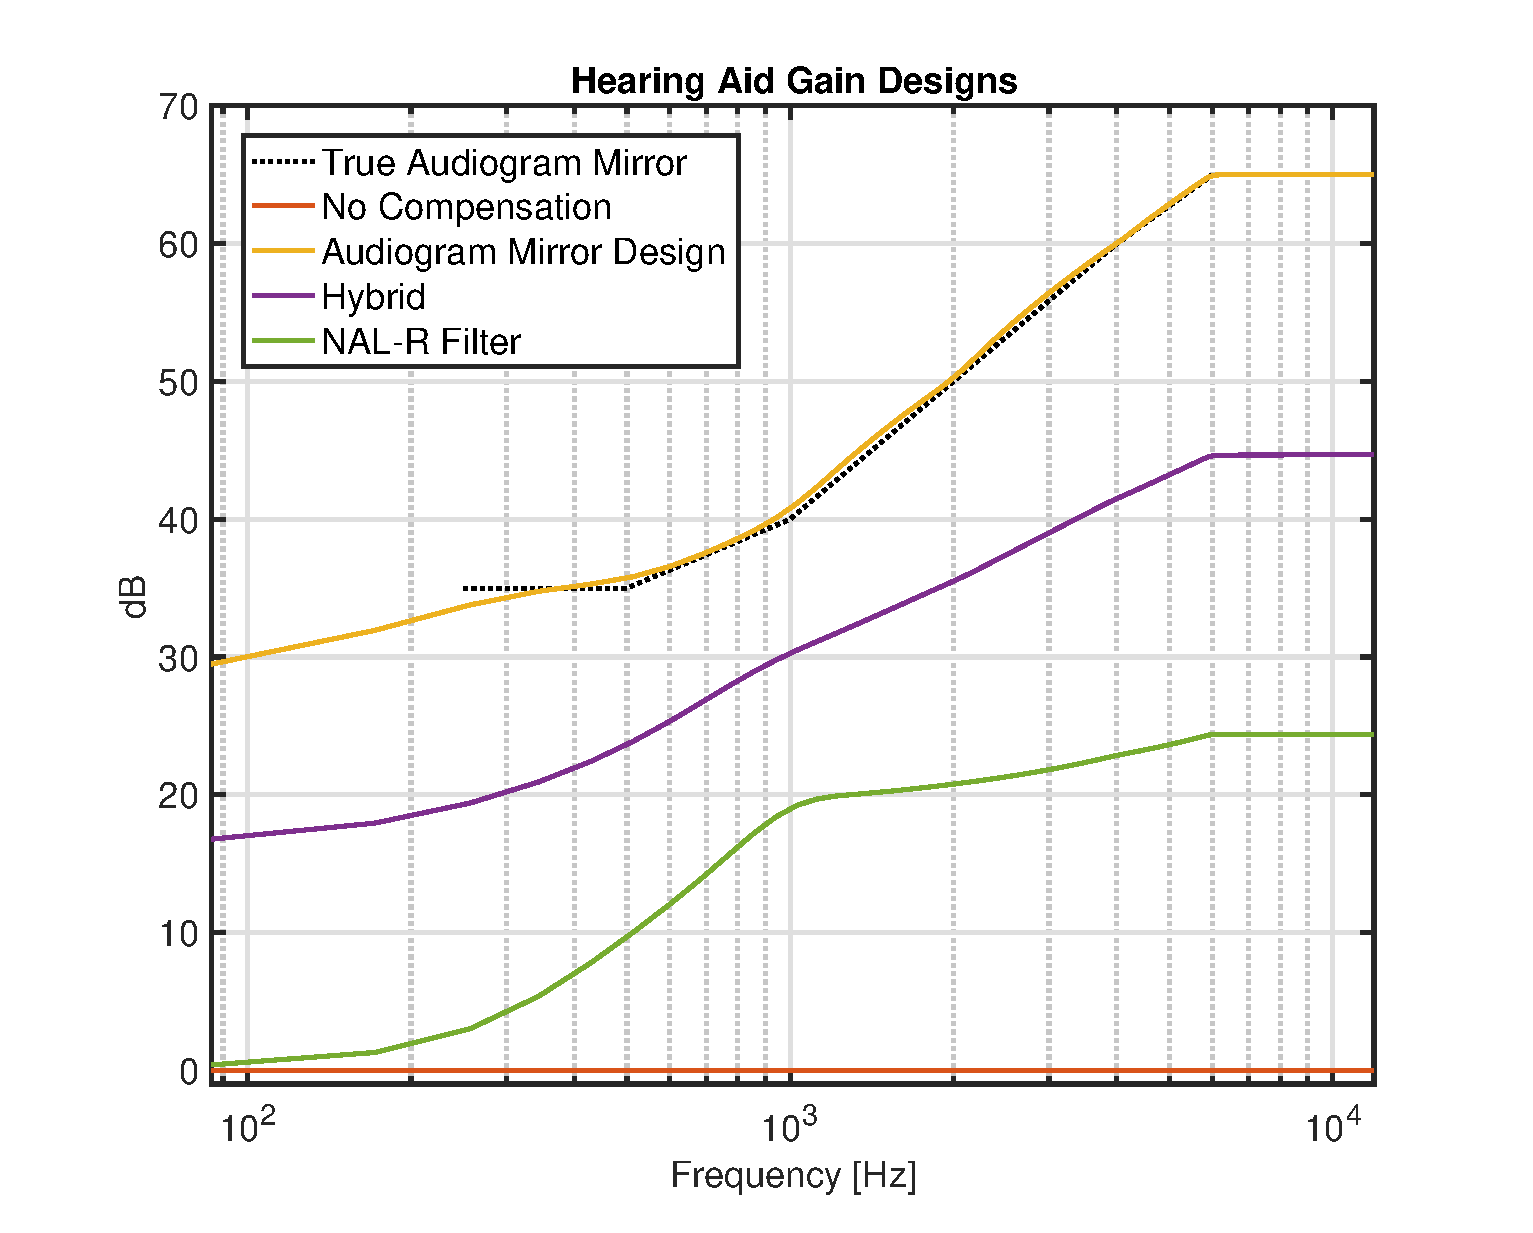
\includegraphics[width=0.7\textwidth]{HearingAidGains}
	\centering
	\caption[Hearing aid gains considered for use in evaluation]{Hearing aid gains used in evaluation. The audiogram corresponds to IEC 60118-15 Moderate HL Moderately Sloping Group \citep{bisgaard2010standard}, and NAL-R refers to the gain proposed by \cite{byrne1986national}.}
	\label{fig:HA_Gains}
\end{figure}

\begin{figure}[H]
	\centering
	\begin{subfigure}[b]{0.49\textwidth}
		\centering
		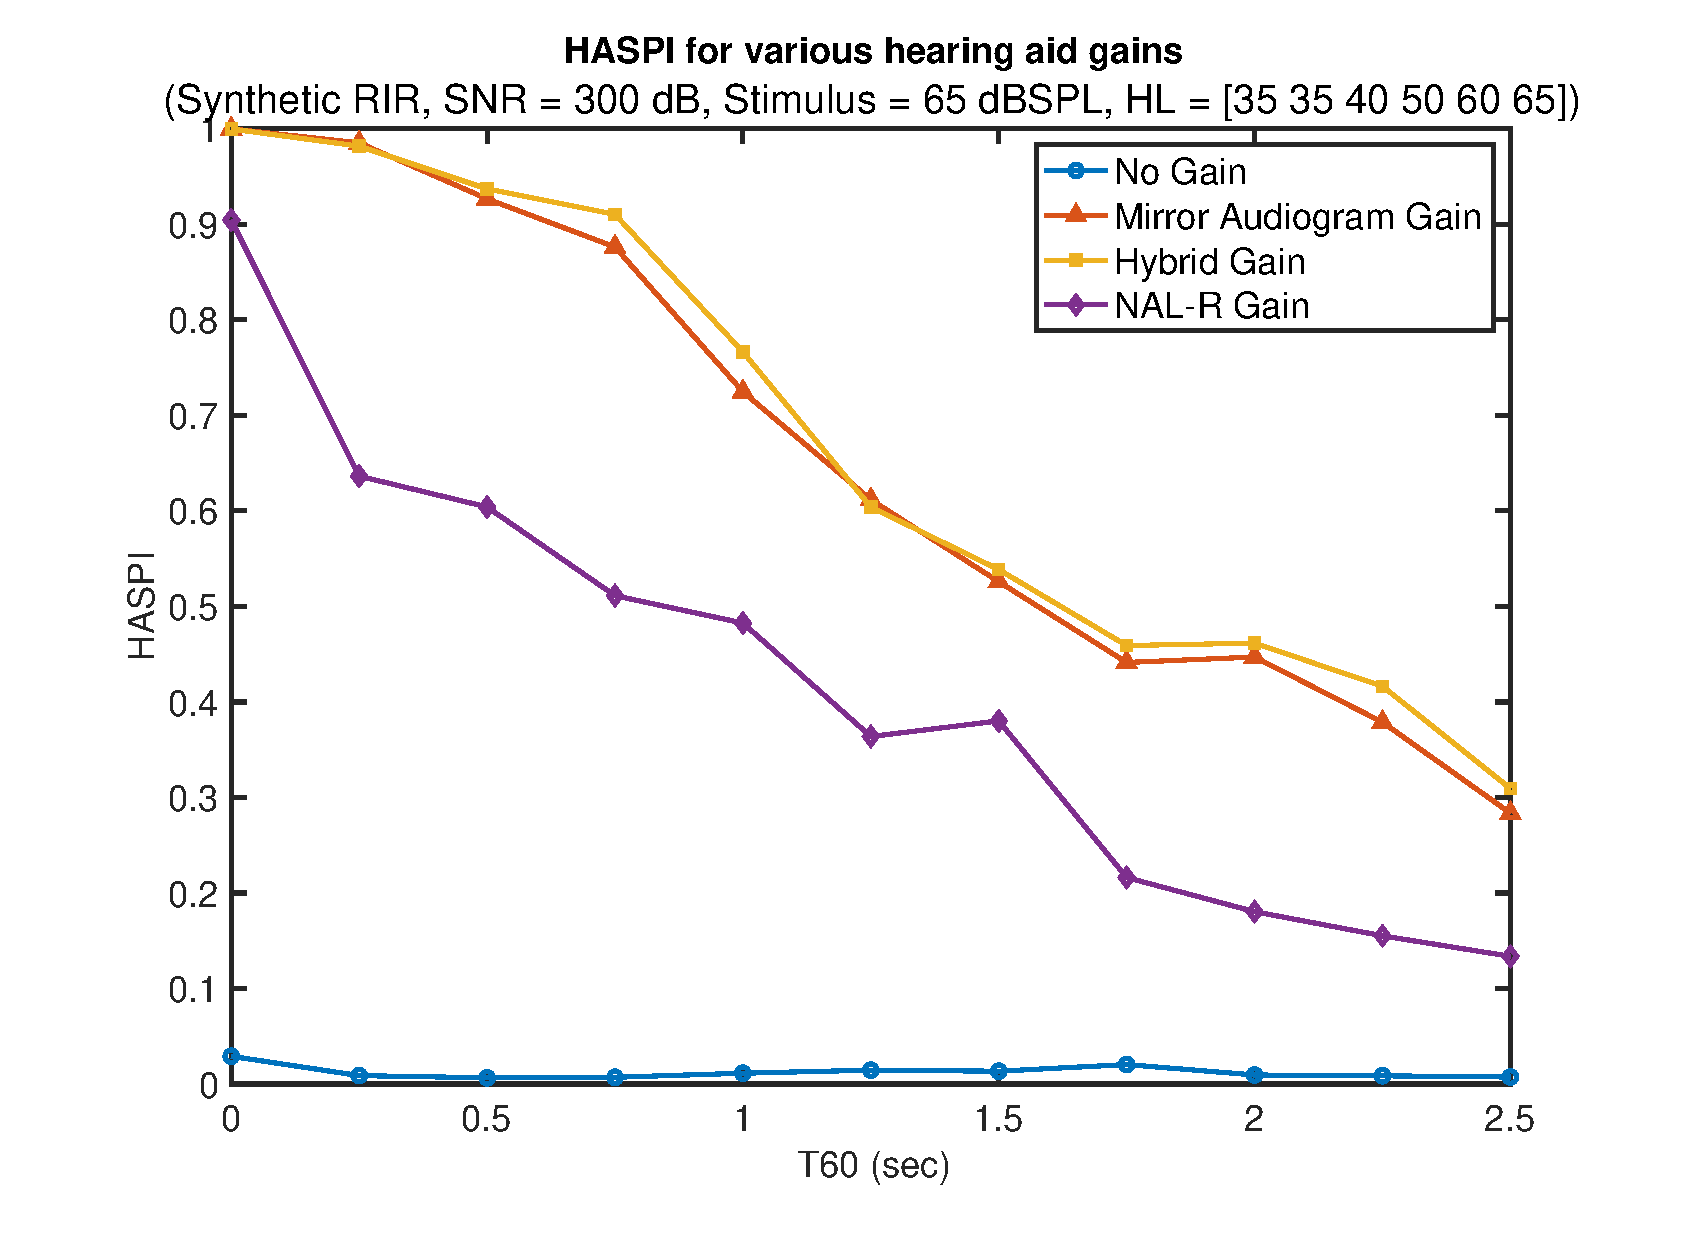
\includegraphics[width=\textwidth]{HASPI_v_T60_variousHAGains}
		\subcaption{}
		\label{subfig:HA_GainComparison_HASPI}
	\end{subfigure}
	\hfill
	\begin{subfigure}[b]{0.49\textwidth}
		\centering
		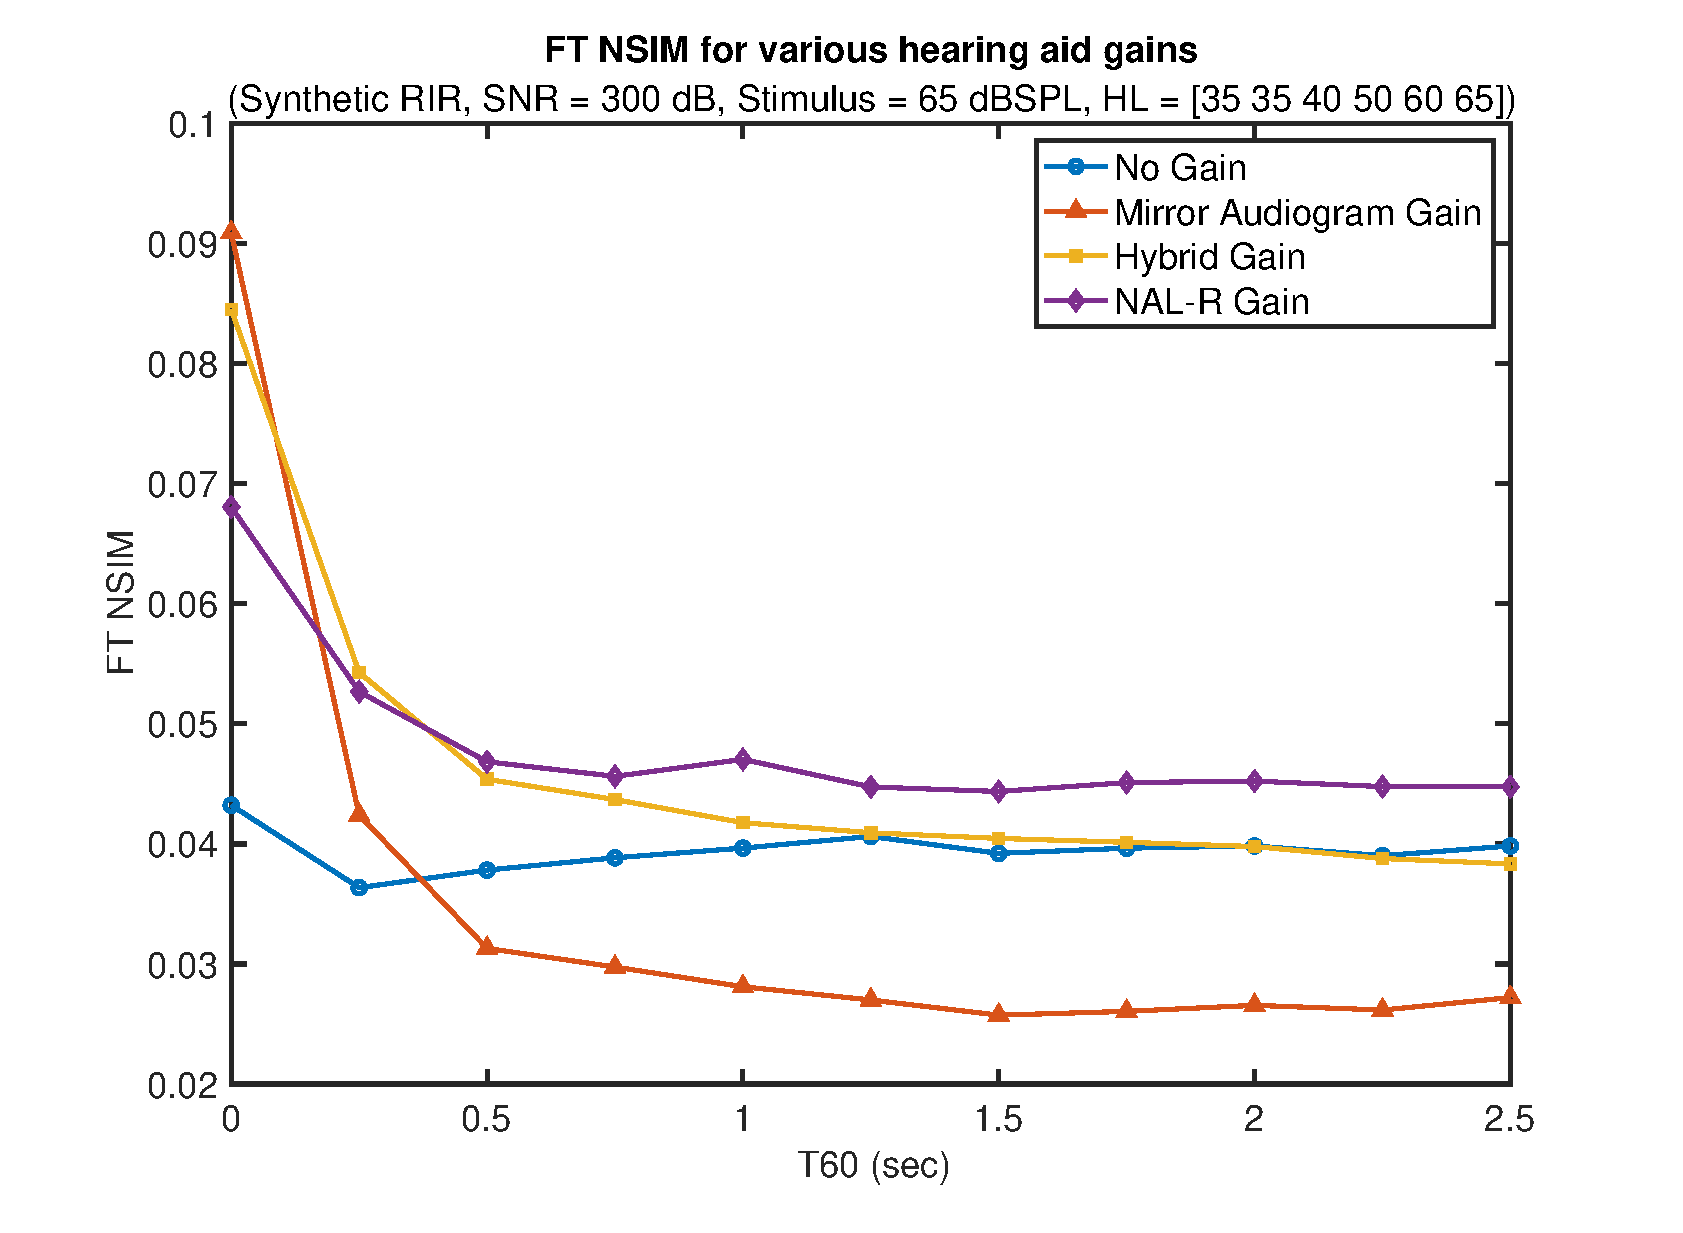
\includegraphics[width=\textwidth]{NSIM_FT_v_T60_variousHAGains}
		\subcaption{}
		\label{subfig:HA_GainComparison_NSIM_FT}
	\end{subfigure}
	\hfill
	\begin{subfigure}[b]{0.49\textwidth}
		\centering
		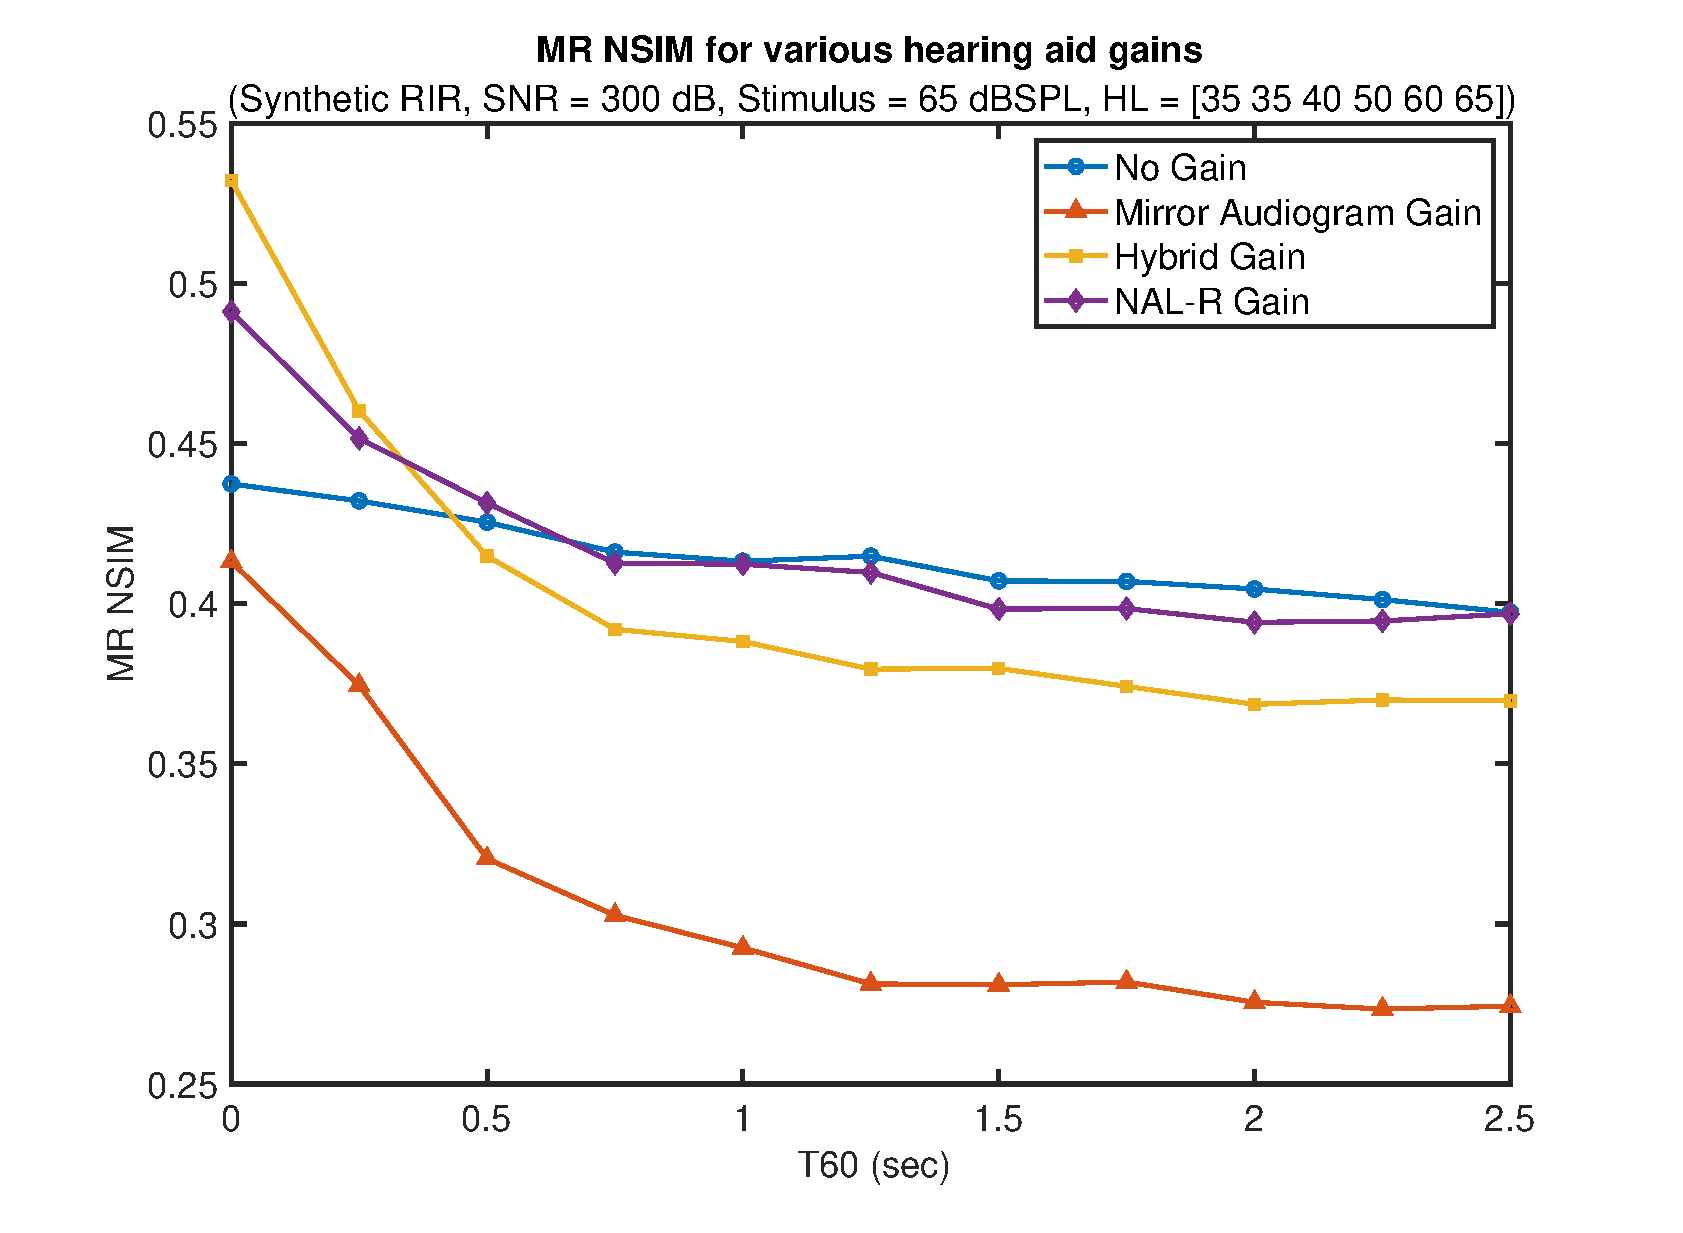
\includegraphics[width=\textwidth]{NSIM_MR_v_T60_variousHAGains}
		\subcaption{}
		\label{subfig:HA_GainComparison_NSIM_MR}
	\end{subfigure}
	\hfill
	\begin{subfigure}[b]{0.49\textwidth}
		\centering
		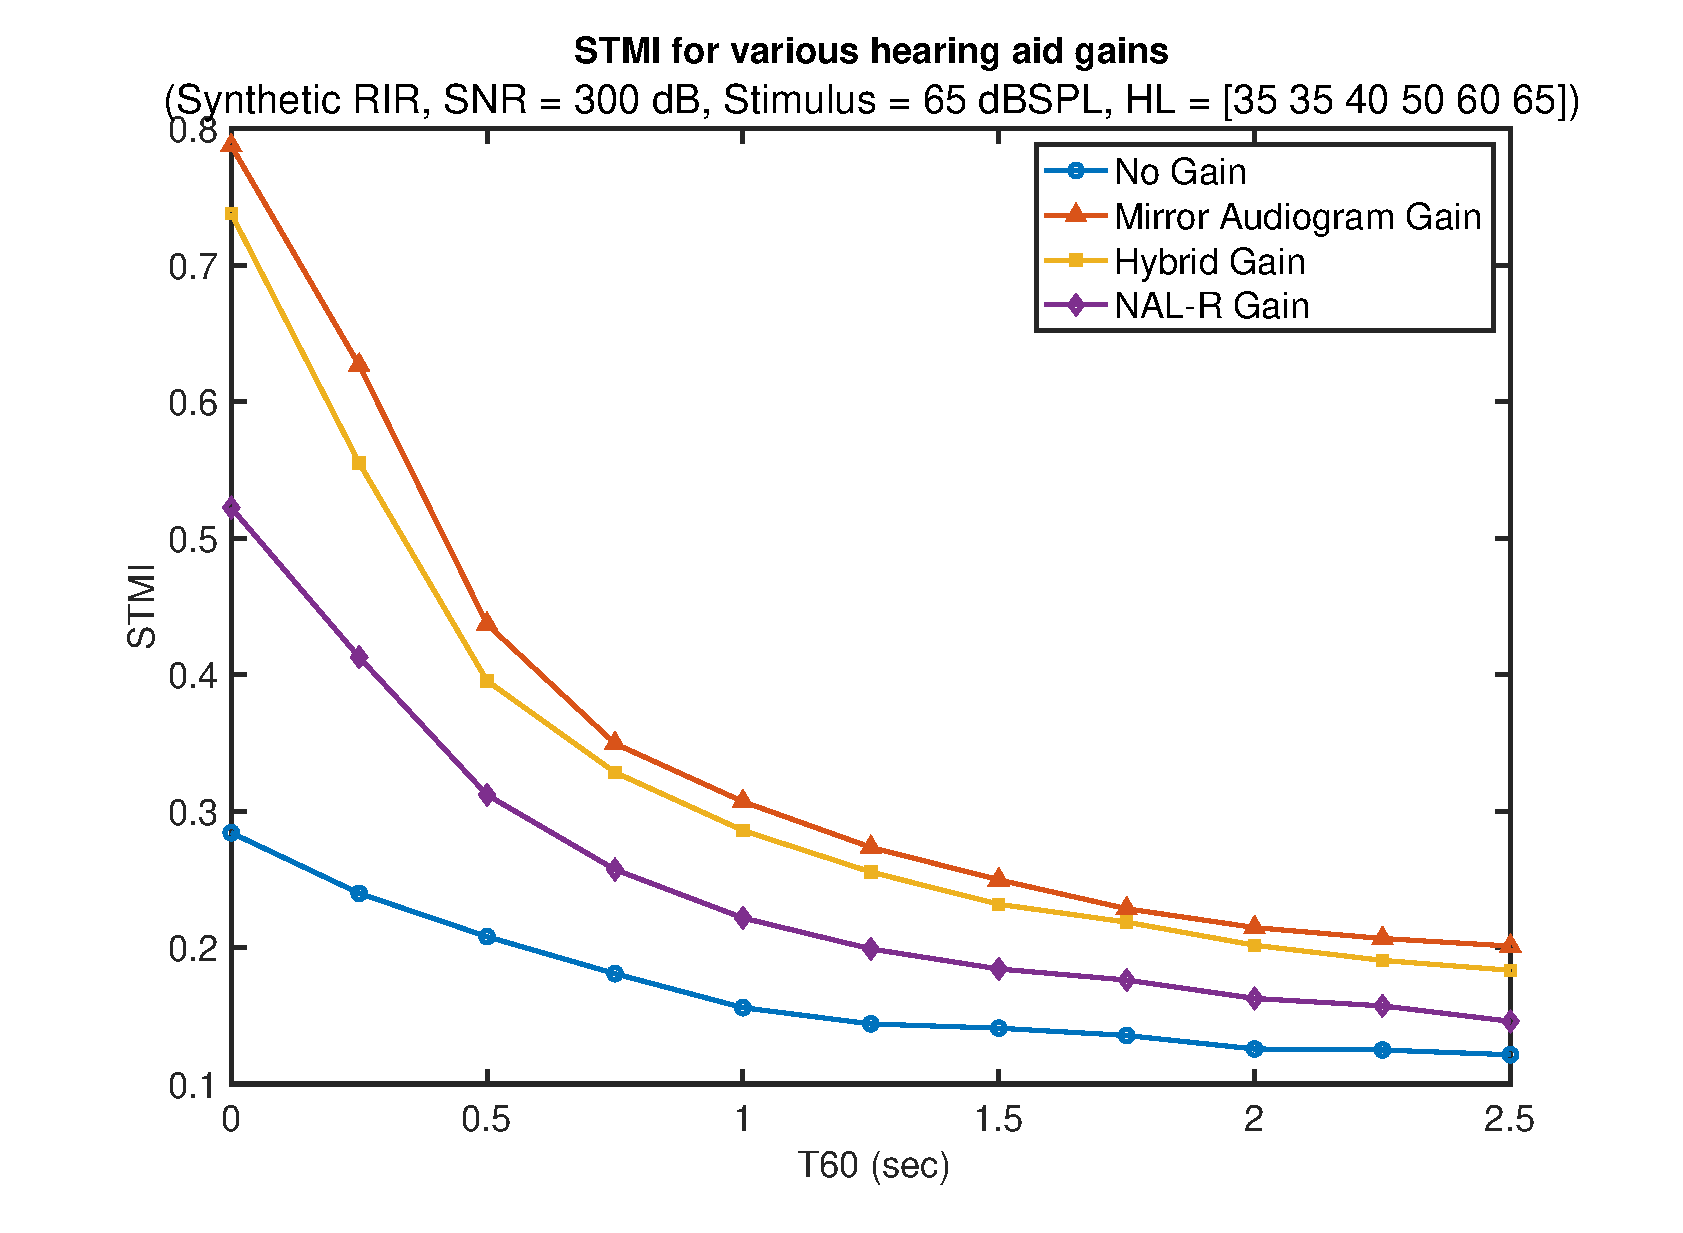
\includegraphics[width=\textwidth]{STMI_v_T60_variousHAGains}
		\subcaption{}
		\label{subfig:HA_GainComparison_STMI}
	\end{subfigure}
	\hfill
	\caption[Comparison of perceptual benefit of hearing aid gains considered for use in evaluation]{Comparison of perceptual benefit of four different linear hearing aid gains in the presence of reverberation. Moderate high frequency hearing loss used in the perceptual models (IEC 60118-15 Moderate HL, Moderately Sloping Group), and RIRs were generated synthetically.}
	\label{fig:HA_GainComparison}
\end{figure}

As seen in Figure \ref{fig:HA_GainComparison}, the intelligibility predictors presented significantly different conclusions on which gain vector was perceptually optimal. This makes sense since each of the predictors is different either in their auditory modeling, or in how the metric is computed from the model output. 

The HASPI results suggested the audiogram mirror to be the best gain vector and no gain to be the worst, regardless of the amount of reverberation. This is likely due to the simpler auditory modeling in HASPI, thus emphasizing audibility over the complexities of non-linear hearing loss. 

In absense of reverberation (i.e., at $\mathrm{T60} = 0 \unit{\sec}$), the MR-NSIM results generally suggested more gain to be more optimal, which aligned with the restoration of ENV cues audibility being achievable by linear amplification with minimal distortion. However, some impacts of distortion at very high sound pressure levels were reflected by the mirror audiogram performing the worst. The FT-NSIM results interestingly suggested more gain to be preferable in absense of reverberation. While this seems converse to the understanding that TFS cues are more severely impacted by auditory non-linearities, it was assumed that this was due to the fact that ... \textbf{Don't have an explanation. In absense of noise/reverberation TFS arent important for intelligibility, but FT-NSIM isnt really a measure of intelligibility, it is an analysis of the fidelity of spike-timing/TFS cues, so it should still show this impact.}. 

In reverberation, both the FT-NSIM and MR-NSIM results suggested the NAL-R gain vector to be optimal, and the audiogram mirror to be the worst. This aligns with the conclusions by \cite{byrne1986national} on the optimality of NAL-R gain in the context of noise masking and shows how the better auditory modeling used in the NSIM/STMI better reflects the non-linearities in the auditory system which result in a roll-off of perceptual performance for higher levels. \textbf{Don't have a good explanation for why MR-NSIM shows negative impact of gain and FT-NSIM shows more positive impact of gain (Seems opposite). Maybe to do with past studies being based on noise not reverb. With reverb, amplification of noise doesnt just fill in gaps more, it blurs cues so the impact is more complex.}

% Note that the MR-NSIM results suggest that the NAL-R gain is no better than providing no gain, while the FT-NSIM suggests the NAL-R gain to be superior. This is likely due to the fact that the MR-NSIM primarily correlates to envelope acoustics which contain higher energy content and therefore do not require as much gain. Conversely, the FT-NSIM is generally more correlated to TFS acoustic cues which contain a wider dynamic range (i.e., contains more quieter sounds which require more gain). --> Not true ENV has wider dynamic range

Interestingly, with and without reverberation, the STMI results suggested the audiogram mirror to be most optimal and no gain to be the least optimal. Like the MR-NSIM, STMI is more correlated to ENV acoustic cues, however STMI is a modulation-sensitive metric and is therefore less sensitive to absolute level. Specifically, while the NSIM has a luminance term which reflects absolute level (i.e., the brightness of the neurogram) in addition to the structure term which reflects modulations (i.e., the visible speech structure in the neurogram), the STMI puts more emphasis on only the modulations visible in the neurogram. Additionally, if the speech stimulus were to be raised above conversational speech levels, a greater roll-off effect would be expected for all three neurogram-based metrics.

Since these results generally agreed with the literature, and since the NAL-R gain is well understood in the field of audiology, it was selected to be used going forward.


\subsection{Evaluation of Monaural Speech Intelligibility Metrics In Context of Reverberation} \label{section:eval_si_metrics}

In this section, the validity of the proposed SI predictors in the context of reverberation was evaluated. As described in Section \ref{section:reverb_si}, \cite{george2010measuring} demonstrated that a T60 of approximately \qty{2}{\sec} results in \qty{50}{\percent} SI for normal-hearing listeners. This was determined via a subjective study using synthetic exponentially decaying Gaussian RIRs. It was also explained that SI can roll off at much lower T60s for hearing-impaired listeners, depending on the particular hearing loss. To validate the chosen SI predictors, each predictor was evaluated as a function of a variable T60 with and without hearing loss. As before, a moderate high frequency hearing loss used in the perceptual models (IEC 60118-15 Moderate HL, Moderately Sloping Group), and NAL-R linear hearing aid amplification was included in the hearing impaired case. To match the methods used by \cite{george2010measuring}, the SI predictors were first evaluated using synthetic exponentially decaying RIRs. The results are shown in Figure \ref{fig:SIMetricsEval_Synthetic}.


\begin{figure}[H]
	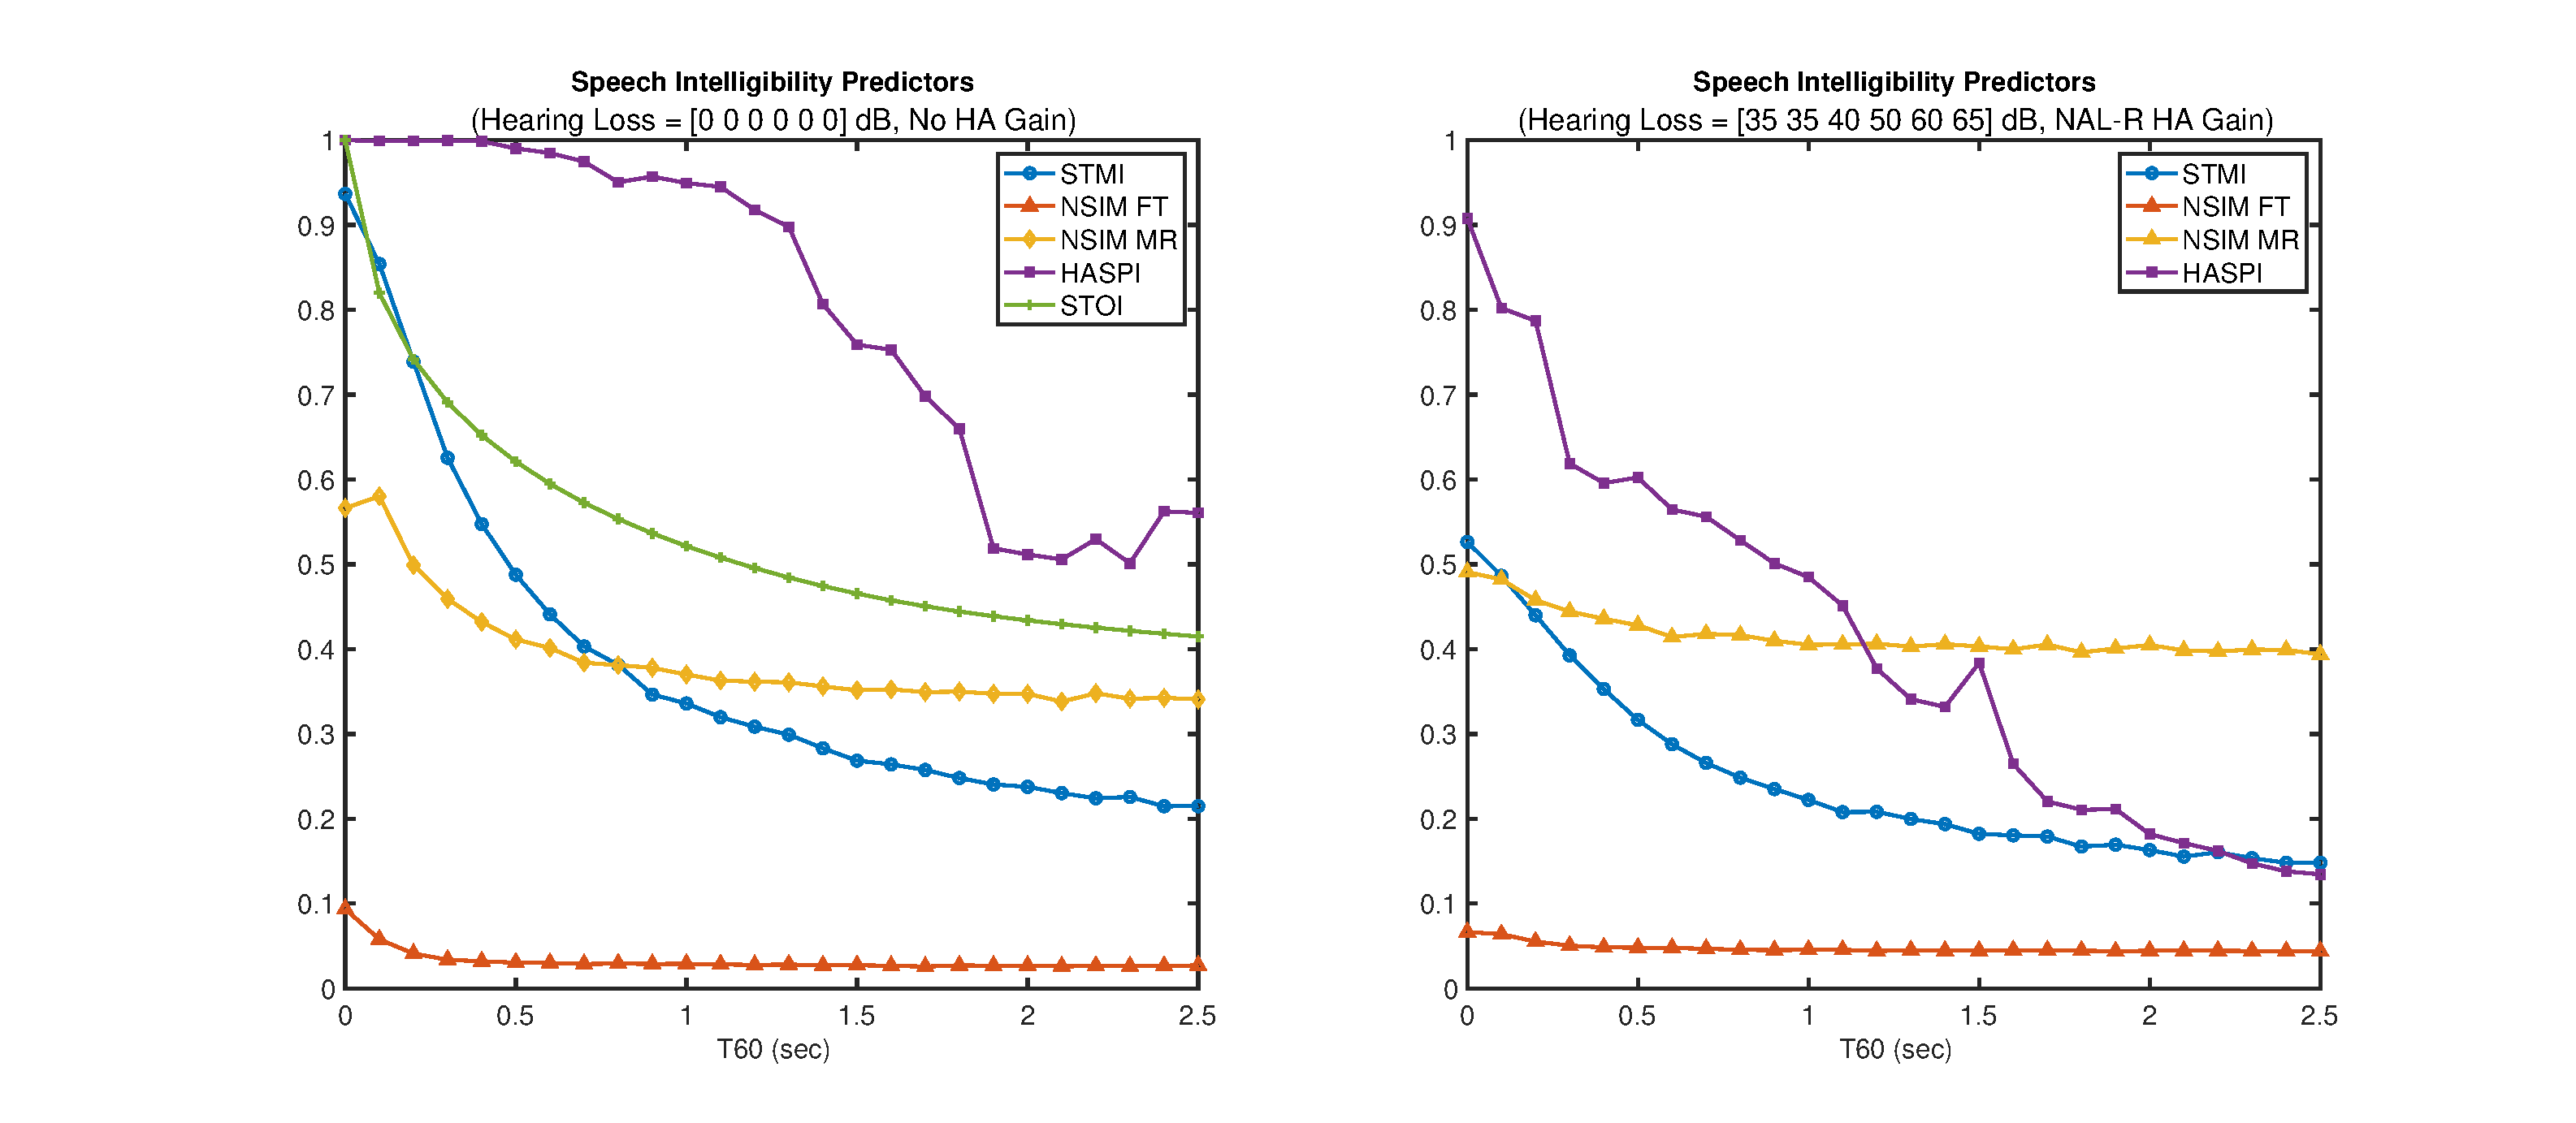
\includegraphics[width=0.98\textwidth]{SIMetricsEval_Synthetic}
	\centering
	\caption[Impact of synthetic reverberation on proposed SI predictors]{Impact of synthetic reverberation (exponentially decaying gaussian RIRs) on SI predictors with and without hearing loss. In the hearing-impaired case, moderate high frequency hearing loss used in the perceptual models (IEC 60118-15 Moderate HL, Moderately Sloping Group), and NAL-R linear hearing aid amplification was included.}
	\label{fig:SIMetricsEval_Synthetic}
\end{figure}

Looking at the normal-hearing case (left), It was first noted that while HASPI and STOI map exactly to a value of 1 for a T60 of \qty{0}{\sec} (i.e., for clean speech), which was expected. However, FT-NSIM, MR-NSIM and STMI all generated a value less than 1 for a T60 of \qty{0}{\sec}. This makes sense because HASPI and STOI have an implicit mapping to SI which scales the predictors appropriately and accounts for floor/ceiling effects. NSIM and STMI have no such mapping and as such can not be directly interpreted as the value of SI.

To better compare all metrics on the same plot, MR-NSIM, FT-NSIM and STMI were scaled by the inverse of their respective value computed at $\mathrm{T60} = \qty{50}{\milli\sec}$ (i.e., direct sound + early reflections) without hearing loss. In other words, the plots are scaled such that the direct sound + early reflections provides a value of 1 for the normal-hearing listener. The results with this scaling are shown in Figure \ref{fig:SIMetricsEval_Synthetic_wScaling}.

\begin{figure}[H]
	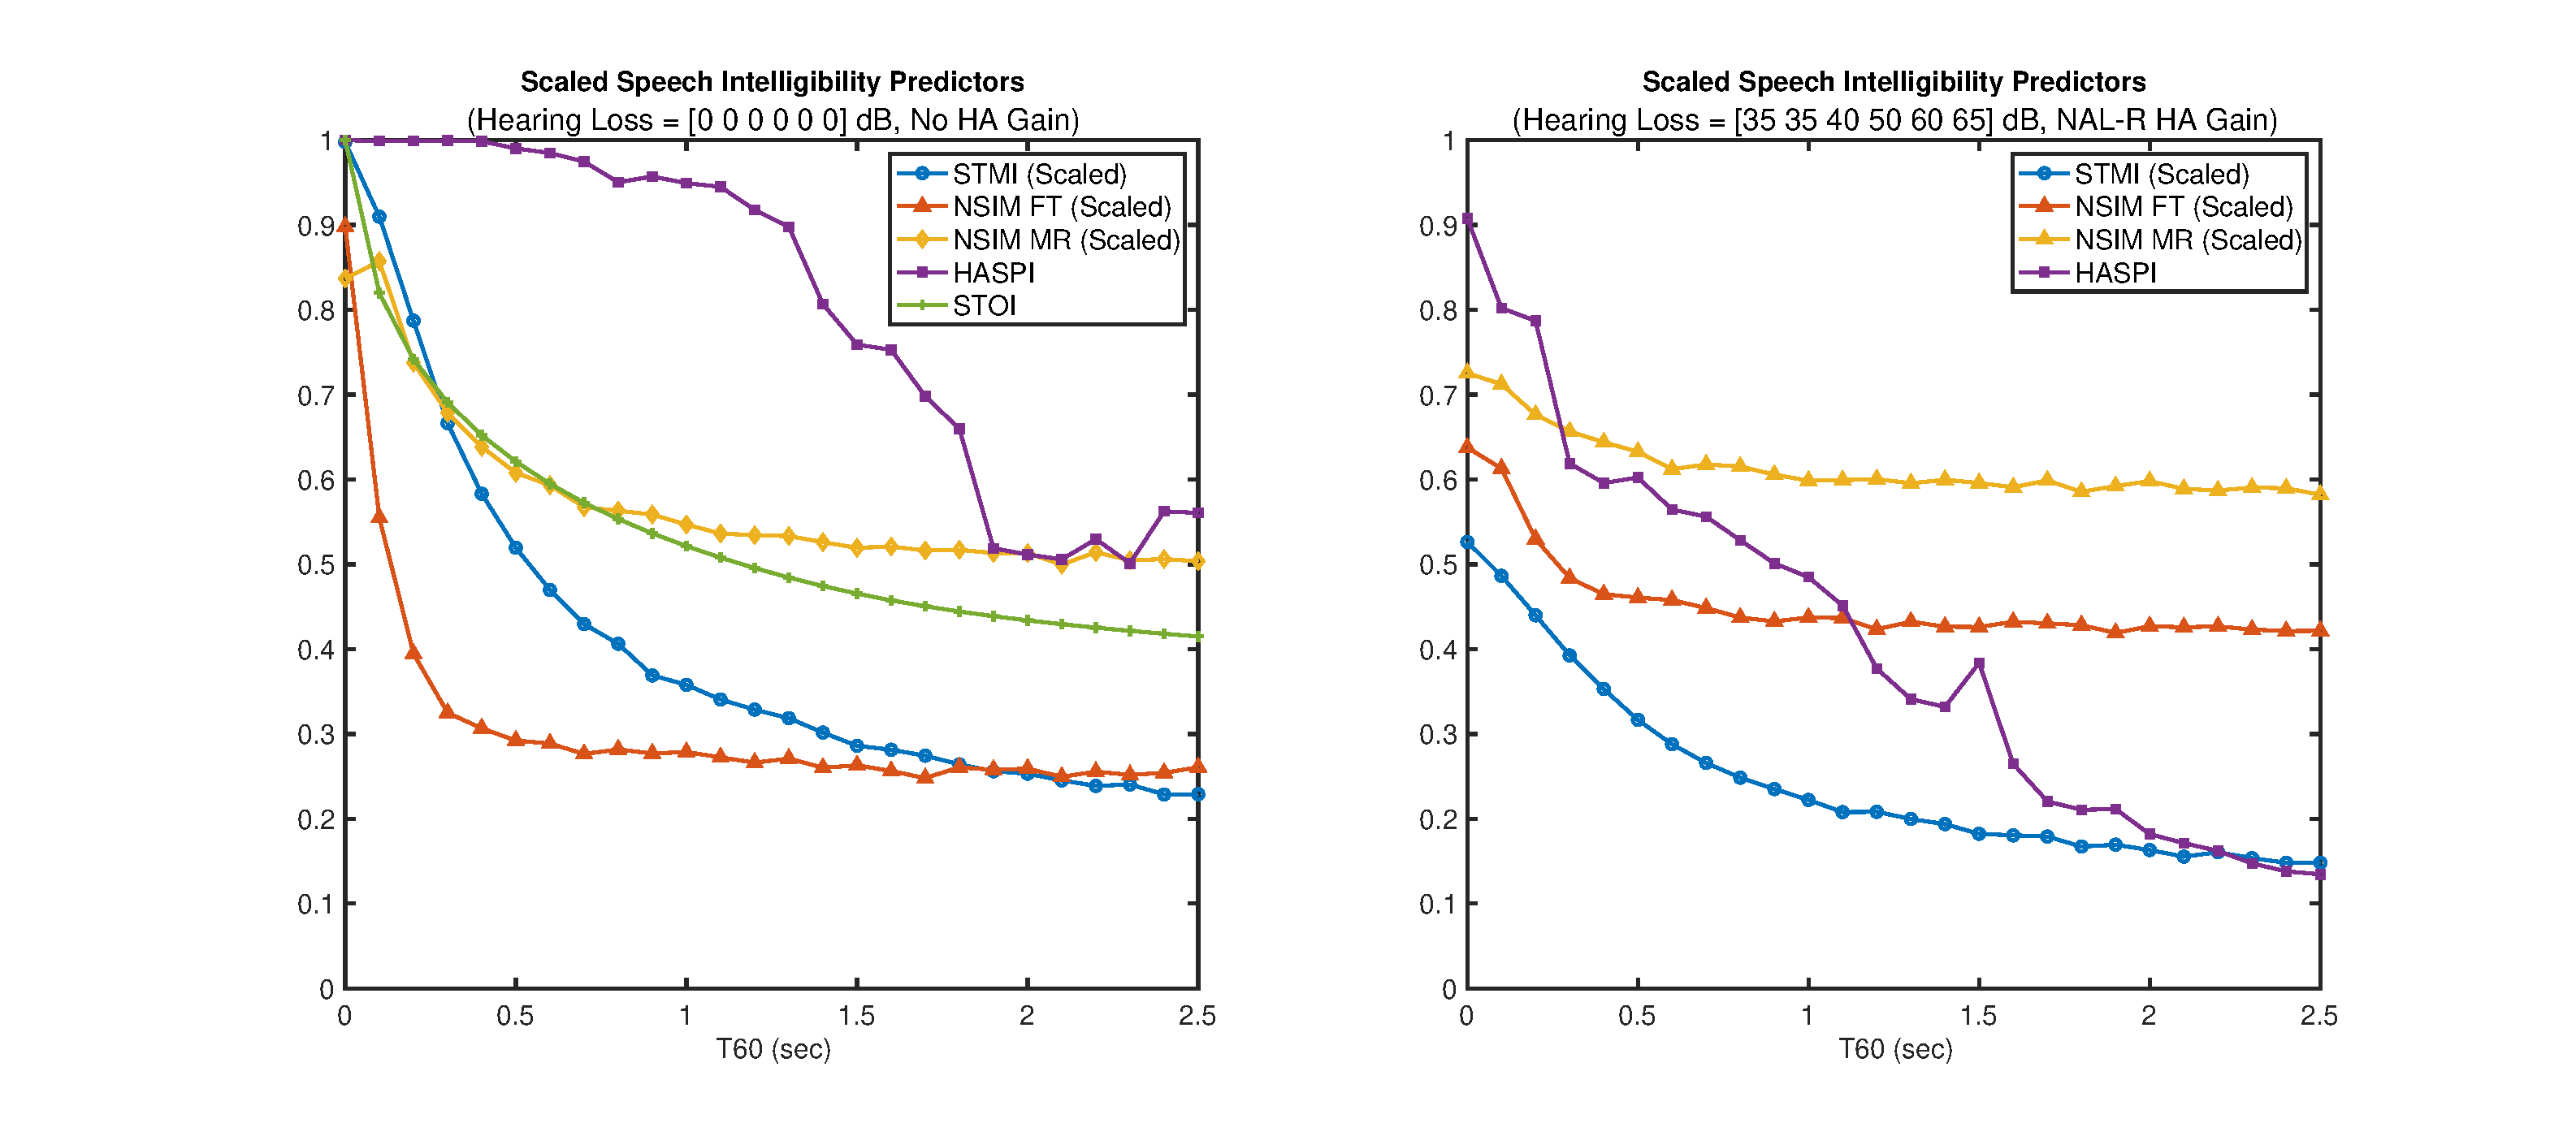
\includegraphics[width=0.98\textwidth]{SIMetricsEval_Synthetic_wScaling}
	\centering
	\caption[Impact of synthetic reverberation on proposed SI predictors (After scaling)]{Impact of synthetic reverberation (exponentially decaying gaussian RIRs) on SI predictors with and without hearing loss. NAL-R linear hearing aid amplification included in hearing loss case for metrics that including modeling of hearing loss. Scaling applied to NSIM and STMI values to better view all metrics on the same plot.}
	\label{fig:SIMetricsEval_Synthetic_wScaling}
\end{figure}

From the normal-hearing case in Figure \ref{fig:SIMetricsEval_Synthetic_wScaling} (left), HASPI, STOI and MR-NSIM all reflect roughly \qty{50}{\percent} of their maximum values at around $\mathrm{T60} = \qty{2}{\sec}$, aligning with the observations of \cite{george2010measuring}. However, STMI and FT-NSIM fall by \qty{50}{\percent} for much shorter T60s, especially FT-NSIM. The severe impact of even mild amounts of reverberation on FT-NSIM reflects the blurring TFS acoustic cues which require very fine temporal resolution to resolve, as described in Section \ref{section:encoding_acoustic_cues}. This is an example of how a combination of MR-NSIM/STMI (which correlate mainly to ENV acoustic cues) with FT-NSIM (which correlates mainly to TFS acoustic cues) provides a more complete picture of the imacts of reverberation on speech perception as discussed in Section \ref{section:neurological_si}. While a significant amount of reverberation is required to obscure speech sufficiently that it impacts SI, even small amounts of reverberation blur the rapidly varying TFS cues which can make perception a more challenging (i.e., impacting LE). As expected, all metrics show worse perception quality accross the board when a hearing-impairment is included (right plot in Figure \ref{fig:SIMetricsEval_Synthetic_wScaling}).

Additionally, while HASPI follows an approximately reverse-sigmoidal pattern due to saturation of SI, all other metrics follow a roughly-exponential decay over the full range of T60s. This demonstrates how the exclusion of an explicit non-linear mapping to SI allows metrics such as NSIM and STMI to show impacts on perception beyond the saturation points of SI (i.e., can be correlated to LE). It should be noted however that some saturation is implicit in the perceptual model used in NSIM and STMI \citep{bruce2018phenomenological} which results in a slight leveling out of the metrics at very low T60s.

In Figure \ref{fig:SIMetricsEval_Real_wScaling}, this experiment was repeated with real RIR measurements of various T60s taken from the MYRiAD and HRIR databases discussed in Section \ref{section:rir_databases}. The results were plotted against the T30s described in Table \ref{table:rir_reverb_times} rather than the T60s. 

% Note that NSIM and STMI have no enforcing of floor/ceiling effects (except those implicit to perceptual saturations in the auditory model), which allows them to reflect LE and not just SI.

%\begin{figure}[H]
%	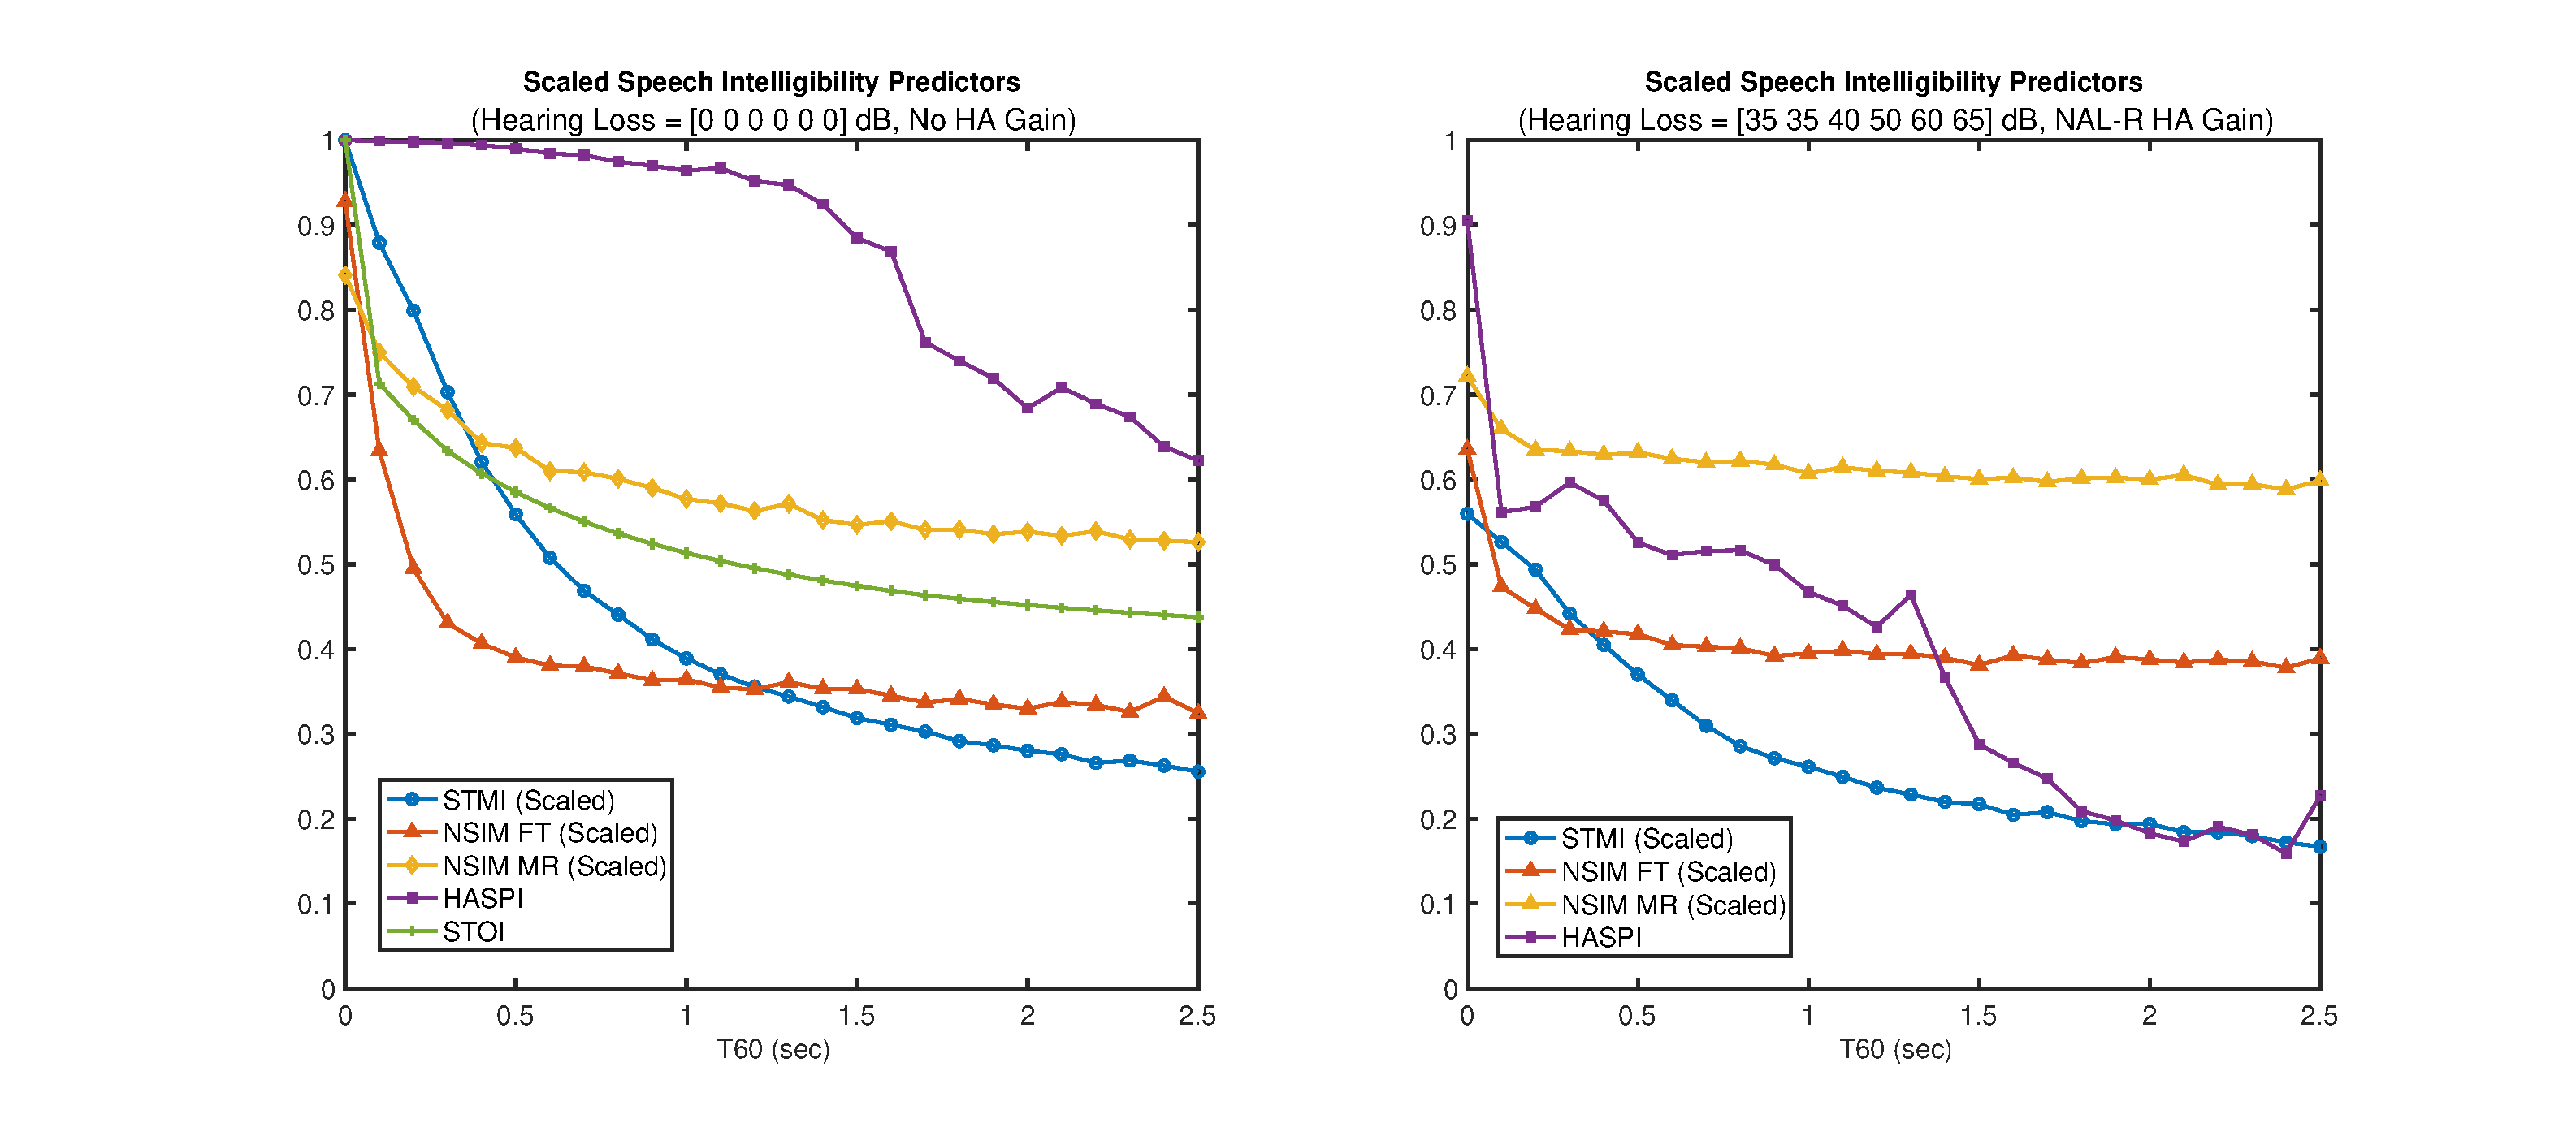
\includegraphics[width=0.98\textwidth]{SIMetricsEval_Synthetic_RealER_wScaling}
%	\centering
%	\caption{Impact of synthetic reverberation (exponentially decaying gaussian RIRs) with added real early reflections generated by truncating a real RIR  (Office II RIR from the HRIR database) on SI predictors with and without hearing loss. NAL-R linear hearing aid amplification included in hearing loss case for metrics that including modeling of hearing loss. Scaling applied to NSIM and STMI values to better view all metrics on the same plot.}
%	\label{fig:SIMetricsEval_Synthetic_RealER_wScaling}
%\end{figure}

\begin{figure}[H]
	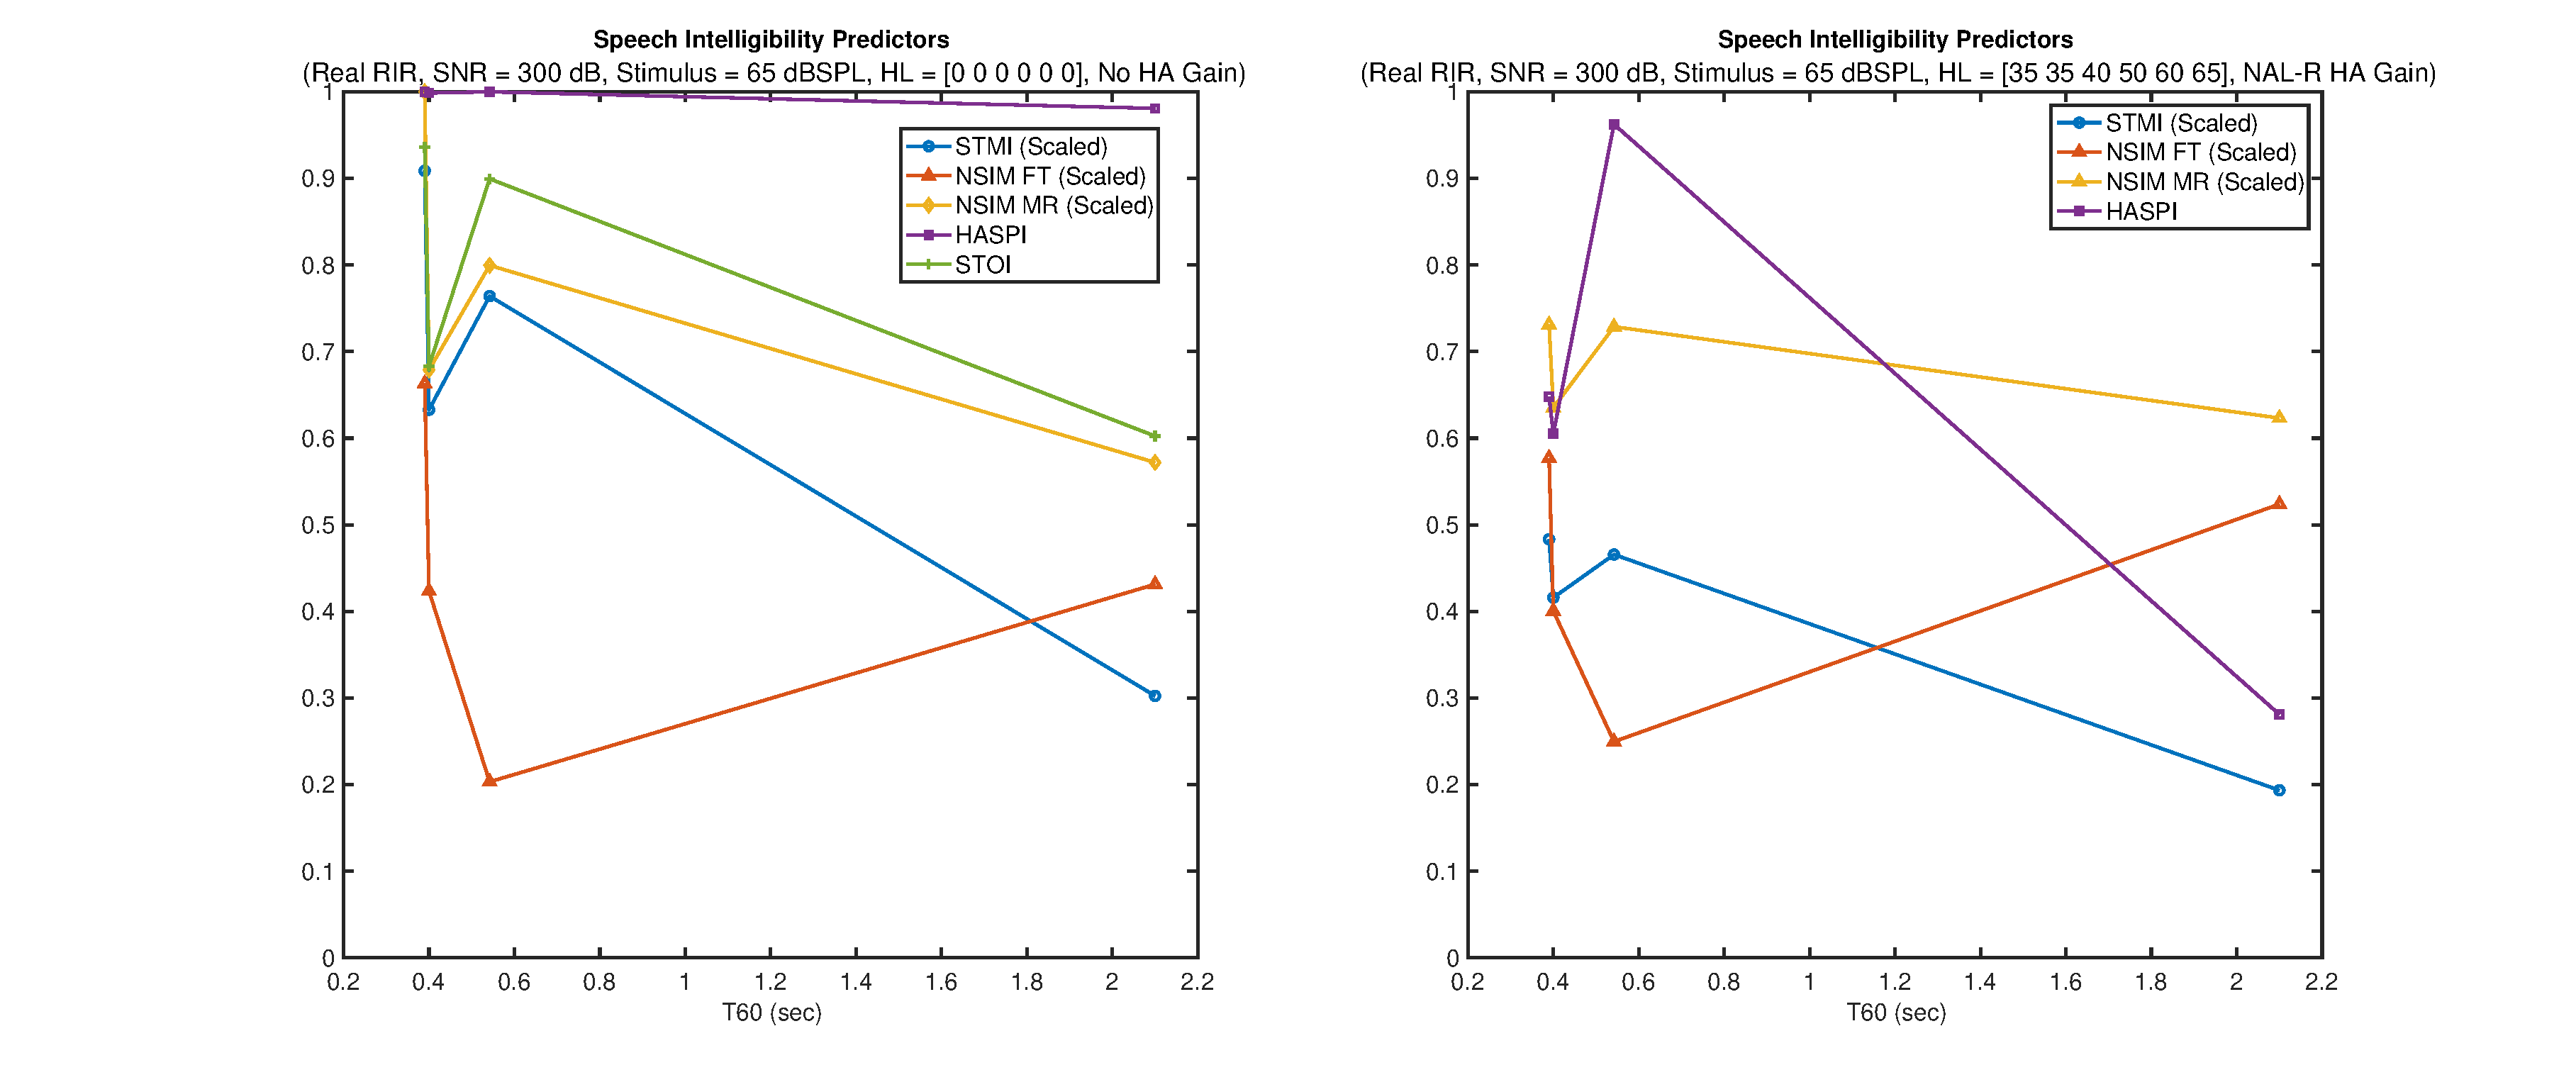
\includegraphics[width=0.98\textwidth]{SIMetricsEval_Real_wScaling}
	\centering
	\caption[Impact of real RIRs on proposed SI predictors (after scaling)]{Impact of practical reverberation (several real measured RIRs) on SI predictors with and without hearing loss. NAL-R linear hearing aid amplification included in hearing loss case for metrics that including modeling of hearing loss.  Scaling applied to NSIM and STMI values to better view all metrics on the same plot.}
	\label{fig:SIMetricsEval_Real_wScaling}
\end{figure}


Note that none of the metrics decay monotonically with T30. This demonstrates how reverberation time provides an incomplete depiction of the perceptual impacts of reverberation due to the different decay rates of the early decay region and late decay region. As discussed in Section \ref{section:early_late_reverb}, a more complete description would include both reverberation time and early decay time (EDT). The early decay region of the SAL RIR from the MYRiAD database (Figure \ref{fig:RIR_EDC_SAL}), which has $\mathrm{T30} = \qty{2.1}{\sec}$, is much stronger than the late decay region. Conversely, the cafeteria RIR from the HRIR database (Figure \ref{fig:RIR_EDC_Cafeteria}), has a much lower T30 of \qty{542}{\milli\second}, but has much a stronger early decay region. Even though the SAL RIR has a longer reverberation time than the cafeteria RIR, the reverberant tail overall is weaker in the SAL room, thus reducing the perceptual reverberant effect of the room. This also explains why in Figure \ref{fig:SIMetricsEval_Real_wScaling} when T30 was increased from \qty{542}{\milli\sec} to \qty{2.1}{\sec}, STMI and MR-NSIM decreased but FT-NSIM actually increased. ENV acoustic cues are only signifantly impacted by the long-term smearing caused by longer/stronger late decay region, while TFS acoustic cues are more also impacted by the presence of a strong early decay region of the RIR due to their rapid time-variance. 

Recall as mentioned in Section \ref{section:early_late_reverb}: the early decay region of the RIR, which is described by the EDT, is distinct in its definition and perceptual impact from the distinction between early/late reflections. EDT and reverberation time  are used to described the two different decay regions of an RIR (loosely referred to in this thesis as the ``early decay region" and ``late decay region"), whereas early/late reflections are a perceptual concept. 


MR-NSIM, STMI, HASPI and STOI were however all found to decay monotonically with C50. This makes sense because C50 is a more perceptually-motivated metric considering the ratio between perceptually ``useful" energy to perceptually ``detrimental". FT-NSIM was not found to vary monotonically with T30, C50 or EDT. This is perhaps due to certain reflection delay ranges having a more pronounced effect on TFS information (e.g., reflections at the word/syllable rate). Further investgiation into this matter was left for a future study.


To analyze the impact on perception of variable amounts of realistic reverberation in a consistent/controllable way, the SAL RIR from the MYRiAD database was exponentially windowed to manipulate the T60. An example of this procedure is shown in Figure \ref{fig:SALTruncationExample}, where the original T60 of \qty{2.2}{\sec} was exponentially windowed to a T60 of \qty{1}{\sec}.

%The decay rate of the exponential window was selected in each case by computing the EDC of the original RIR, computing the difference (in \unit{\decibel}) between the value of the original EDC at the desired T60 and \qty{60}{\decibel}, then computing the window function via:

%\begin{equation}
%	w_{\mathrm{exp}}(n) = e ^ {-n/\tau} = e ^ {-n / \left((\mathrm{T60} \cdot f_s) / \ln(G_{\mathrm{added}})\right)}
%\end{equation}

%\noindent
%where $\tau = \left((\mathrm{T60} \cdot f_s) / \ln(G_{\mathrm{added}})\right)$ is the exponential time constant to acheive the required additional attenuation at the desired T60, and $G_{\mathrm{added}}$ is the additional attenuation as  a linear attenuation. I.e., $G_{\mathrm{added}} = \dots$.

\begin{figure}[H]
	\centering
	\begin{subfigure}[b]{0.49\textwidth}
		\centering
		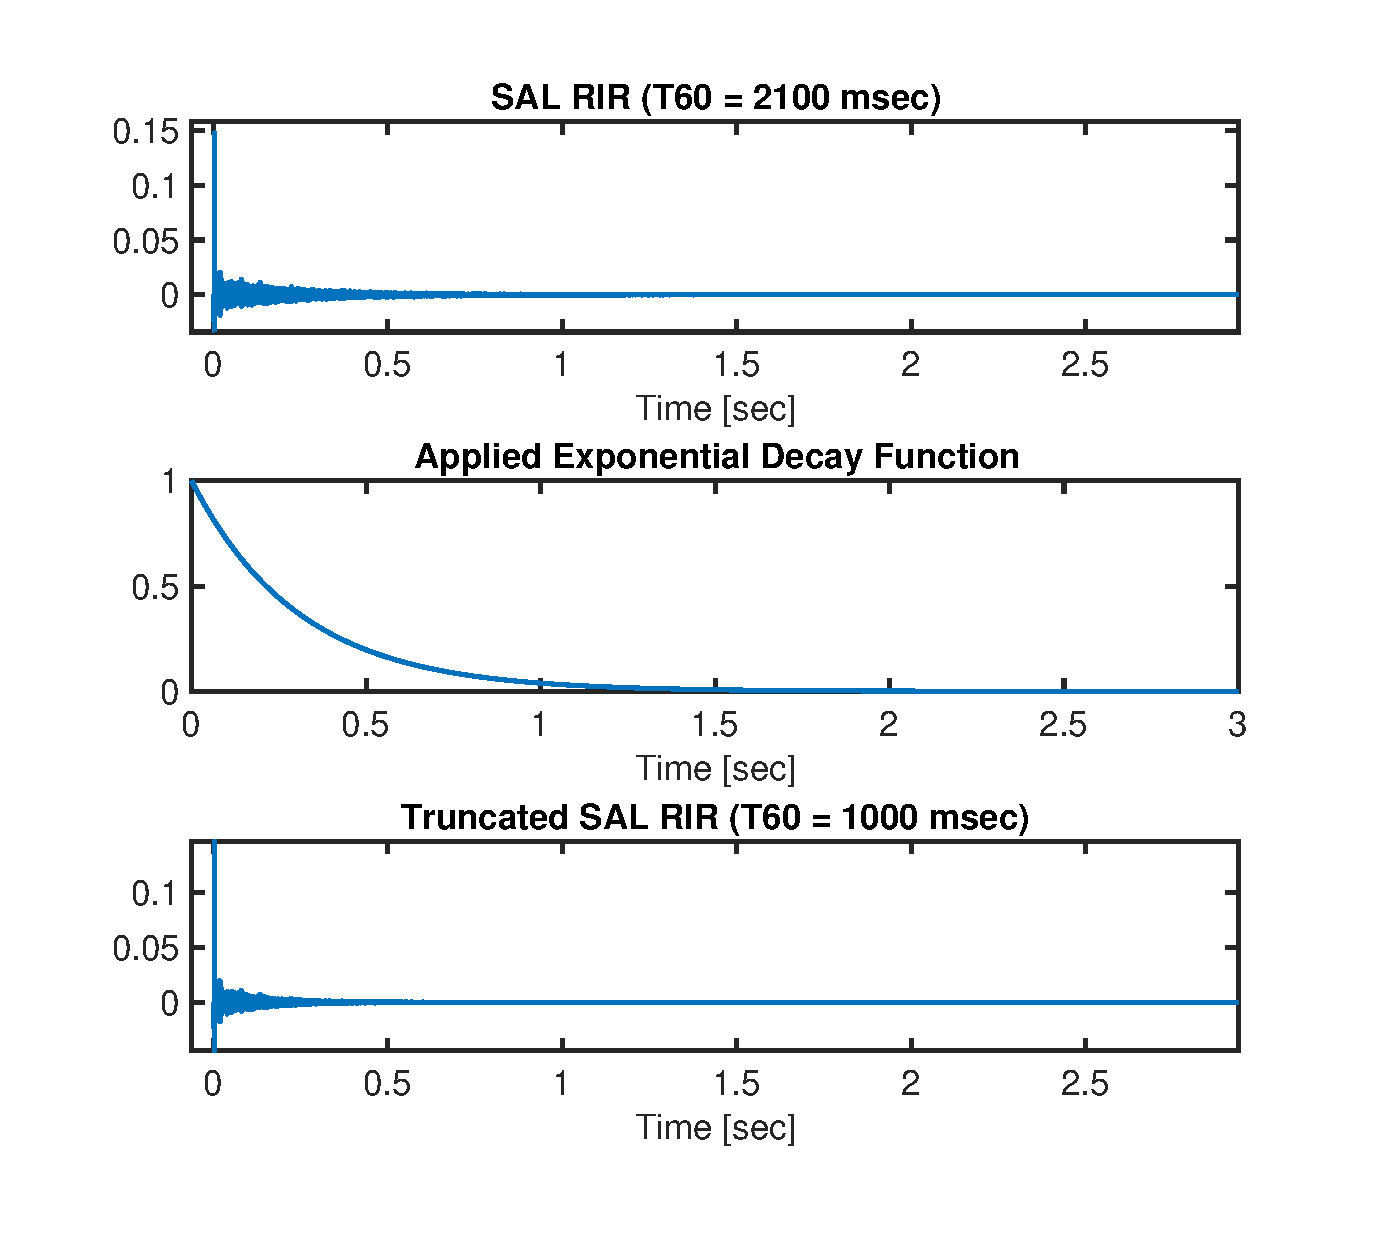
\includegraphics[width=\textwidth]{SALTruncationExample_RIR}
	\end{subfigure}
	\hfill
	\begin{subfigure}[b]{0.49\textwidth}
		\centering
		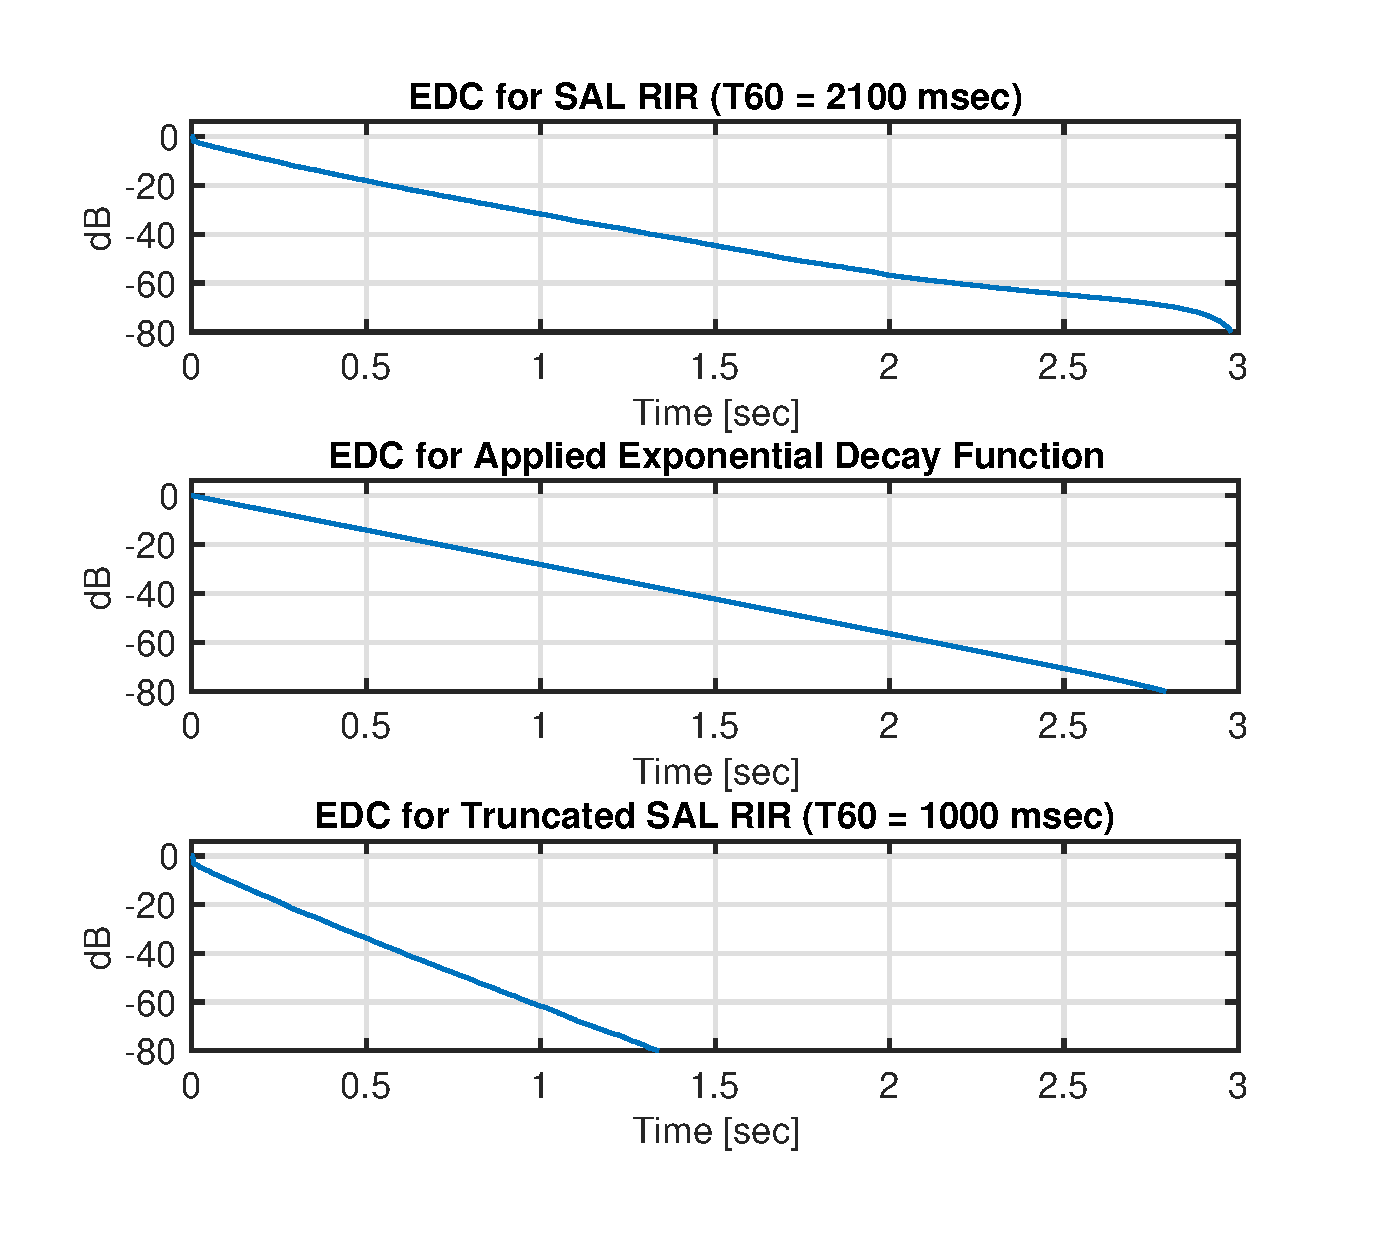
\includegraphics[width=\textwidth]{SALTruncationExample_EDC}
	\end{subfigure}
	\hfill
	\caption[Example of exponential windowing of RIRs to reduce T60]{Example of how SAL was processed by applying additional exponential decay as a window to manipulate T60 synthetically.}
	\label{fig:SALTruncationExample}
\end{figure}

Manipulating the T60 of the SAL RIR in this way, all perceptual metrics were evaluated over a range of T60s. The results are shown in Figure \ref{fig:SIMetricsEval_TruncatedSAL_wScaling}.

\begin{figure}[H]
	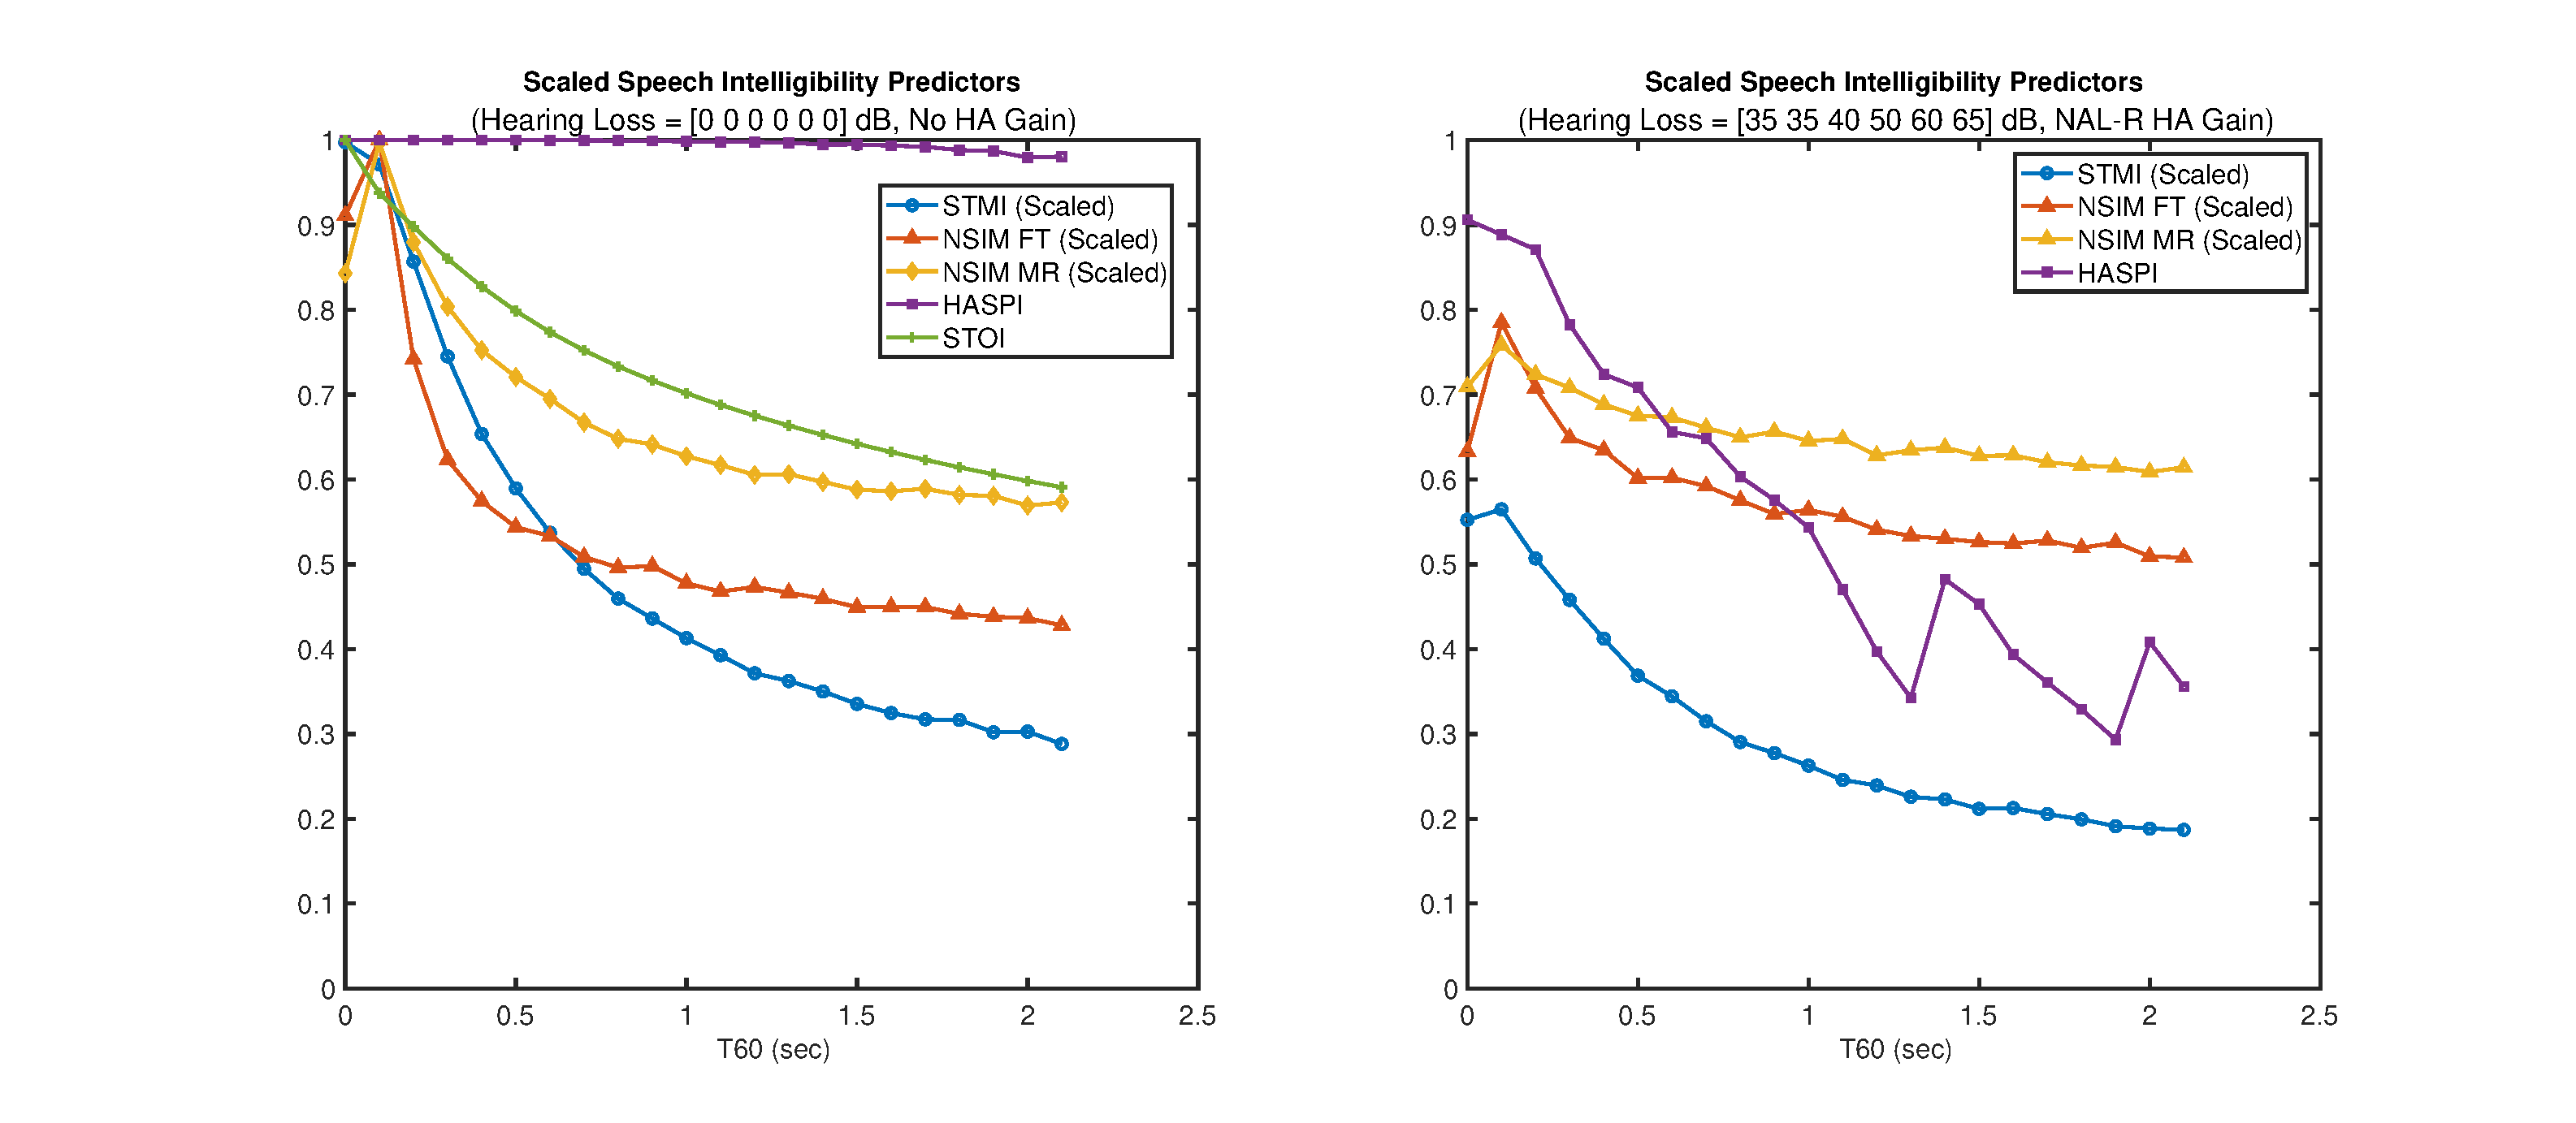
\includegraphics[width=0.98\textwidth]{SIMetricsEval_TruncatedSAL_wScaling}
	\centering
	\caption[Impact of exponentially windowed real RIRs on proposed SI predictors (after scaling)]{Impact of practical reverberation (SAL room from MYRiAD database exponentially truncated to control T60) on SI predictors with and without hearing loss. NAL-R linear hearing aid amplification included in hearing loss case for metrics that including modeling of hearing loss.  Scaling applied to NSIM and STMI values to better view all metrics on the same plot.}
	\label{fig:SIMetricsEval_TruncatedSAL_wScaling}
\end{figure}

In this experiment all metrics were found to decay monotonically with T60, following a similar relation to that which was observed with synthetic RIRs in Figure \ref{fig:SIMetricsEval_Synthetic_wScaling}. Interestingly, in the normal-hearing case HASPI was found to predict effectively \qty{100}{\percent} SI right up to a T60 of \qty{2.1}{\sec}, compared to a prediction of \qty{50}{\percent} SI in the synthetic RIR case (Figure \ref{fig:SIMetricsEval_Synthetic_wScaling}). This is because the synthetic RIRs were generated by using a single exponential decay rate over the full T60, resulting in a much longer EDT and therefore a much louder reverberant tail. This again reinforces the impact of the early decay region on perception. However, the other metrics do not have this saturation, and show variation in speech perception over the full range of T60s, which is expected to correlate to LE as previously discussed.

As a final example of the impact of EDT on speech perception, the same experiment was conducted, but the direct impulse / early reflection impulses were manually attenuated by \qty{6}{\decibel} to increase the EDT slightly (i.e., to increase the late reverberant energy relative to the early decay region). The RIR/EDC for the processed SAL RIR, and the experiment results are shown in Figure \ref{fig:SAL_ERProcessing_Div2} and Figure \ref{fig:SAL_ERProcessing_Div2_SI_Results} respectively.


\begin{figure}[H]
	\centering
	\begin{subfigure}[b]{0.49\textwidth}
		\centering
		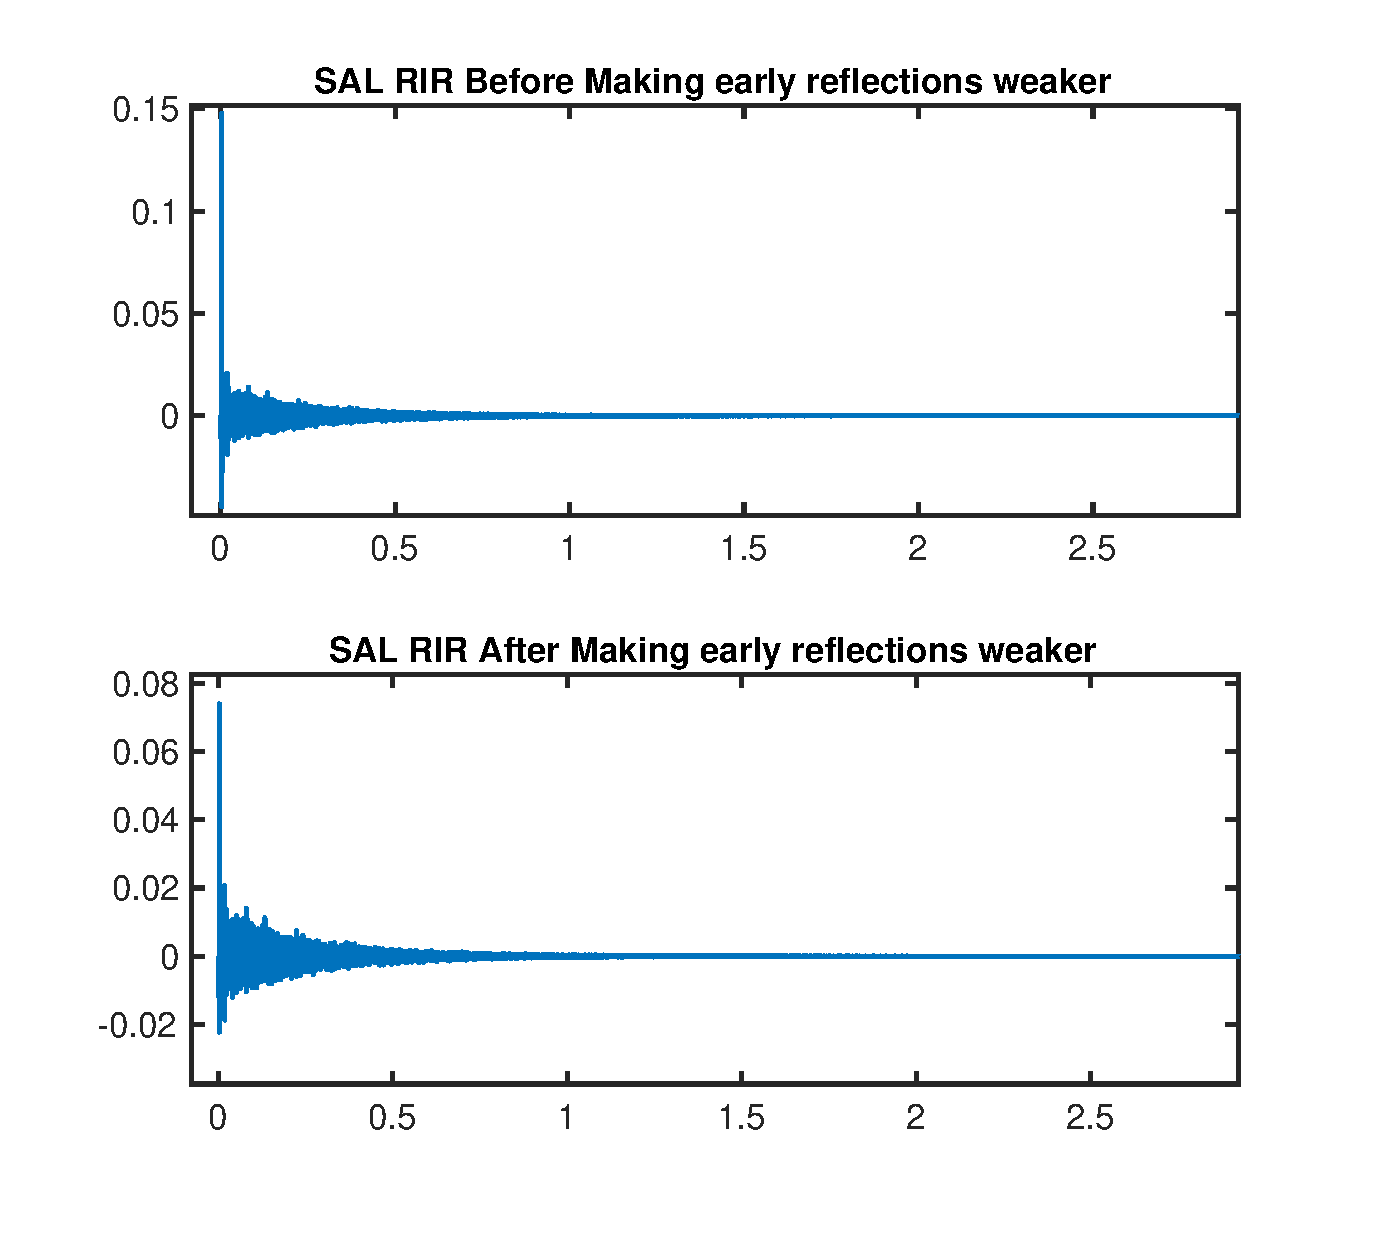
\includegraphics[width=\textwidth]{SAL_ERProcessingExample_Div2_RIR}
	\end{subfigure}
	\hfill
	\begin{subfigure}[b]{0.49\textwidth}
		\centering
		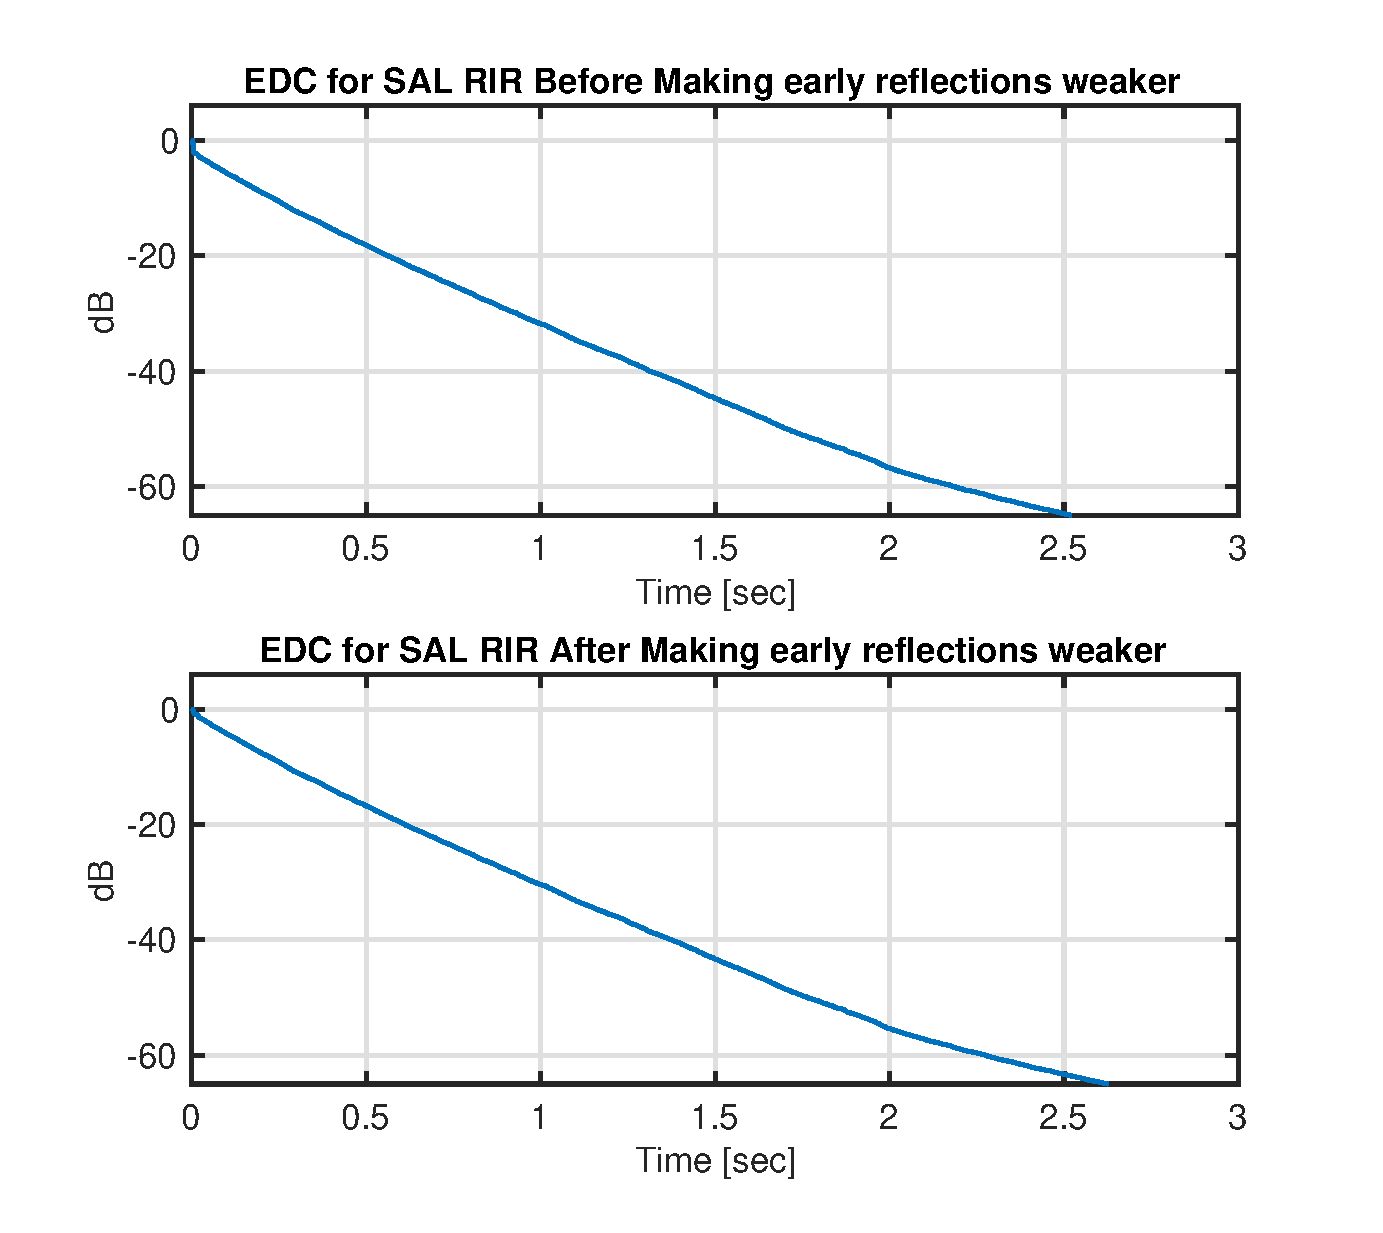
\includegraphics[width=\textwidth]{SAL_ERProcessingExample_Div2_EDC}
	\end{subfigure}
	\caption[Example of reducing prominance of early reflections]{Example of how early reflections of SAL RIR were reduced in magnitude by \qty{6}{\decibel} to make reverberation effect stronger}
	\label{fig:SAL_ERProcessing_Div2}
\end{figure}

\begin{figure}[H]
	\centering
	\begin{subfigure}[b]{0.98\textwidth}
		\centering
		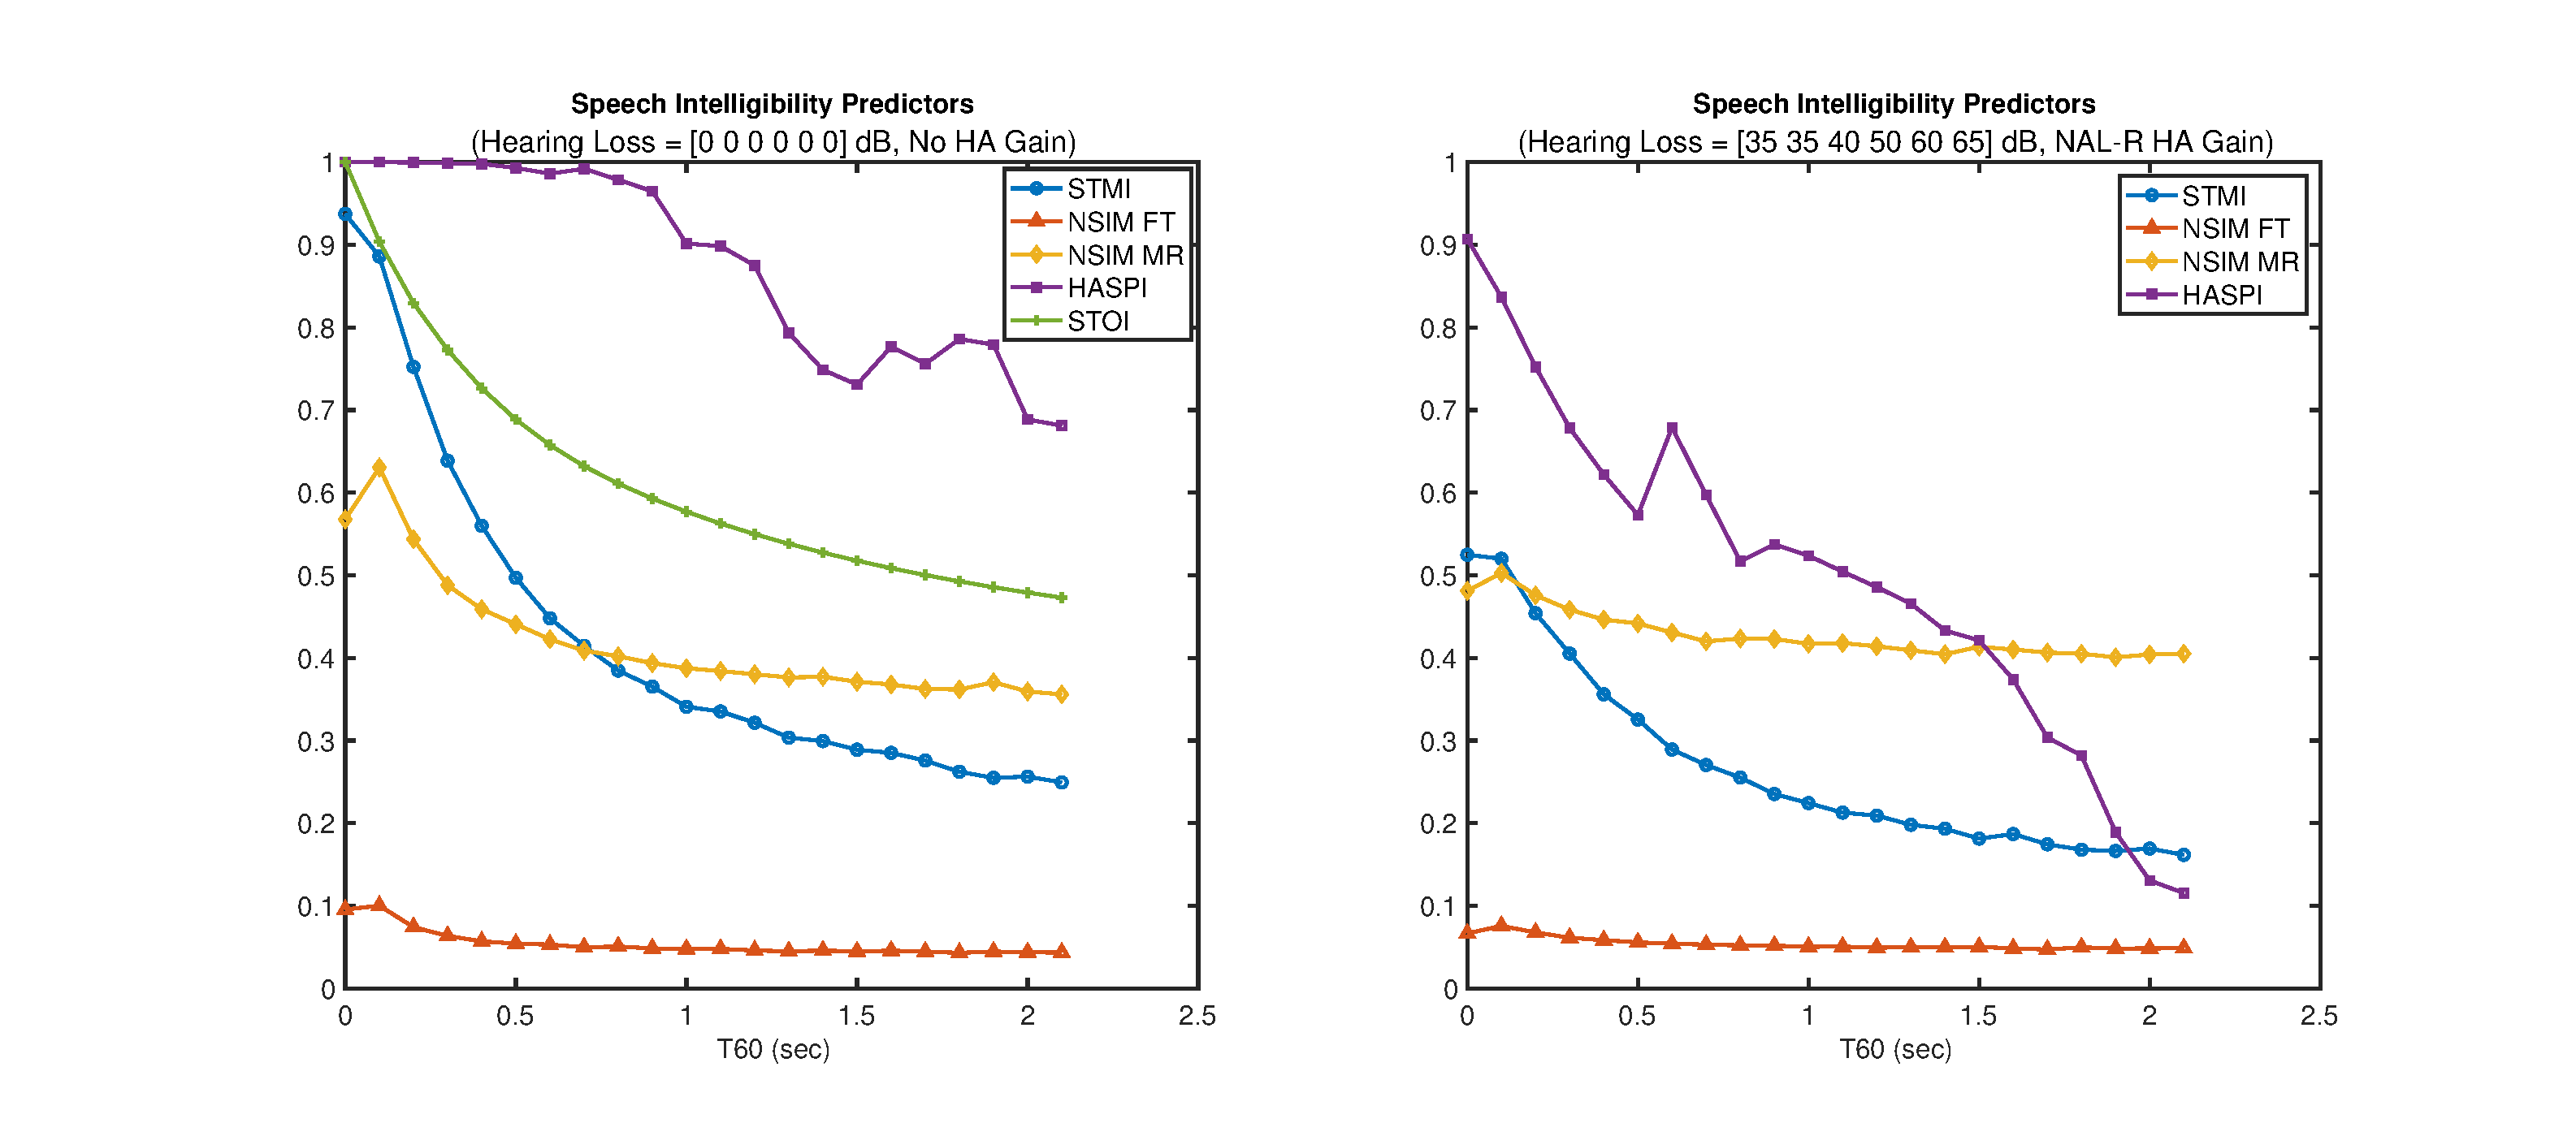
\includegraphics[width=\textwidth]{SAL_ERProcessingExample_Div2_SI}
	\end{subfigure}
	\caption[Impact of exponentially windowed real RIRs with reduced early reflections on proposed SI predictors (after scaling)]{Impact of practical reverberation (SAL room from MYRiAD database exponentially windowed to control T60) on SI predictors with and without hearing loss. NAL-R linear hearing aid amplification included in hearing loss case for metrics that including modeling of hearing loss.  Scaling applied to NSIM and STMI values to better view all metrics on the same plot. The direct sound / early reflections of SAL RIR were reduced by \qty{6}{\decibel} as shown in Figure \ref{fig:SAL_ERProcessing_Div2}.}
	\label{fig:SAL_ERProcessing_Div2_SI_Results}
\end{figure}

With a relatively subtle attenuation of the early reflections (\qty{6}{\decibel}), a very significant change in the perceptual metrics was observed. Note that this pre-processing of the early reflections actually has very minimal impact on the T60. Figure \ref{fig:SAL_ERProcessing_Div2} shows a change in T60 from \qty{2.18}{\sec} to only \qty{2.27}{\sec}. This further reinforces the perceptual importance of EDT, distinct from reverberation time.

Although reverberation time provides an incomplete picture of the perceptual impacts of reverberation, it was still desirable to use T60 as the control variable for the experiments in this thesis going forward since it provides a very easy to understand description of the amount of reverberation. Therefore, it was decided to use RIRs generated by exponentially windowing the SAL RIR from the MYRiAD database as a means to evaluate the perceptual impacts of reverberation (and therefore dereverberation algorithms) under realistic reverberant conditions with controllable T60. By using the same base RIR, the early decay rate and late decay rate remain constant accross all cases, and perceptual metrics decay monotonically.



%%%%%%%%%%%%%%%%%%%%%%%%
% BREAK
%%%%%%%%%%%%%%%%%%%%%%%%

%\begin{figure}[H]
%	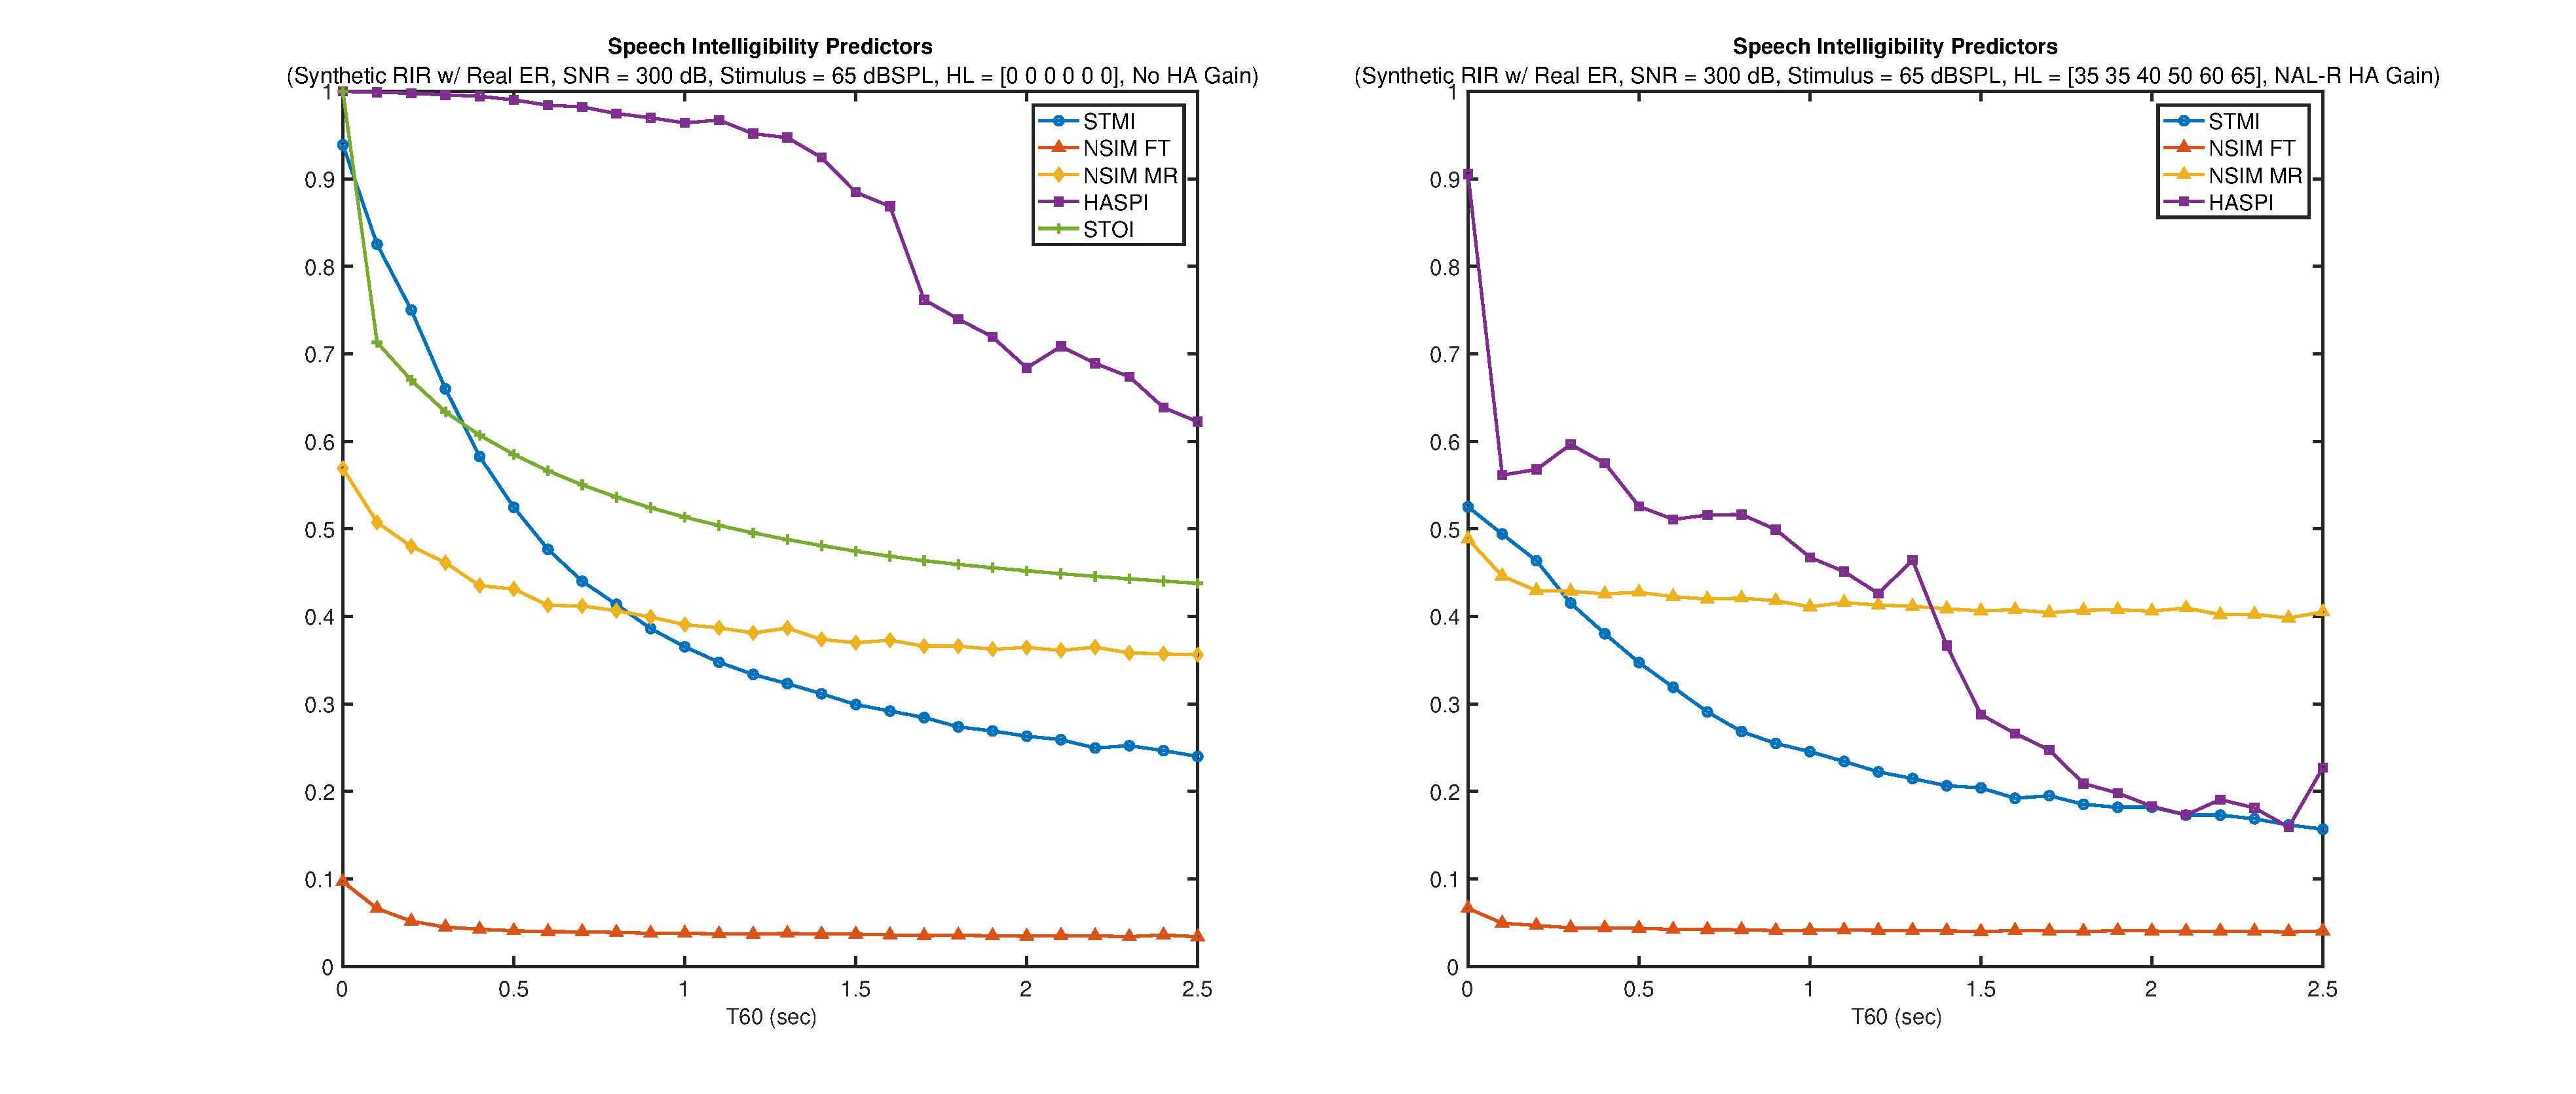
\includegraphics[width=0.98\textwidth]{SIMetricsEval_Synthetic_RealER}
%	\centering
%	\caption{Impact of synthetic reverberation (exponentially decaying gaussian RIRs) with added real early reflections generated by truncating a real RIR  (Office II RIR from the HRIR database) on SI predictors with and without hearing loss. NAL-R linear hearing aid amplification included in hearing loss case for metrics that including modeling of hearing loss}
%	\label{fig:SIMetricsEval_Synthetic_RealER}
%\end{figure}

%\begin{figure}[H]
%	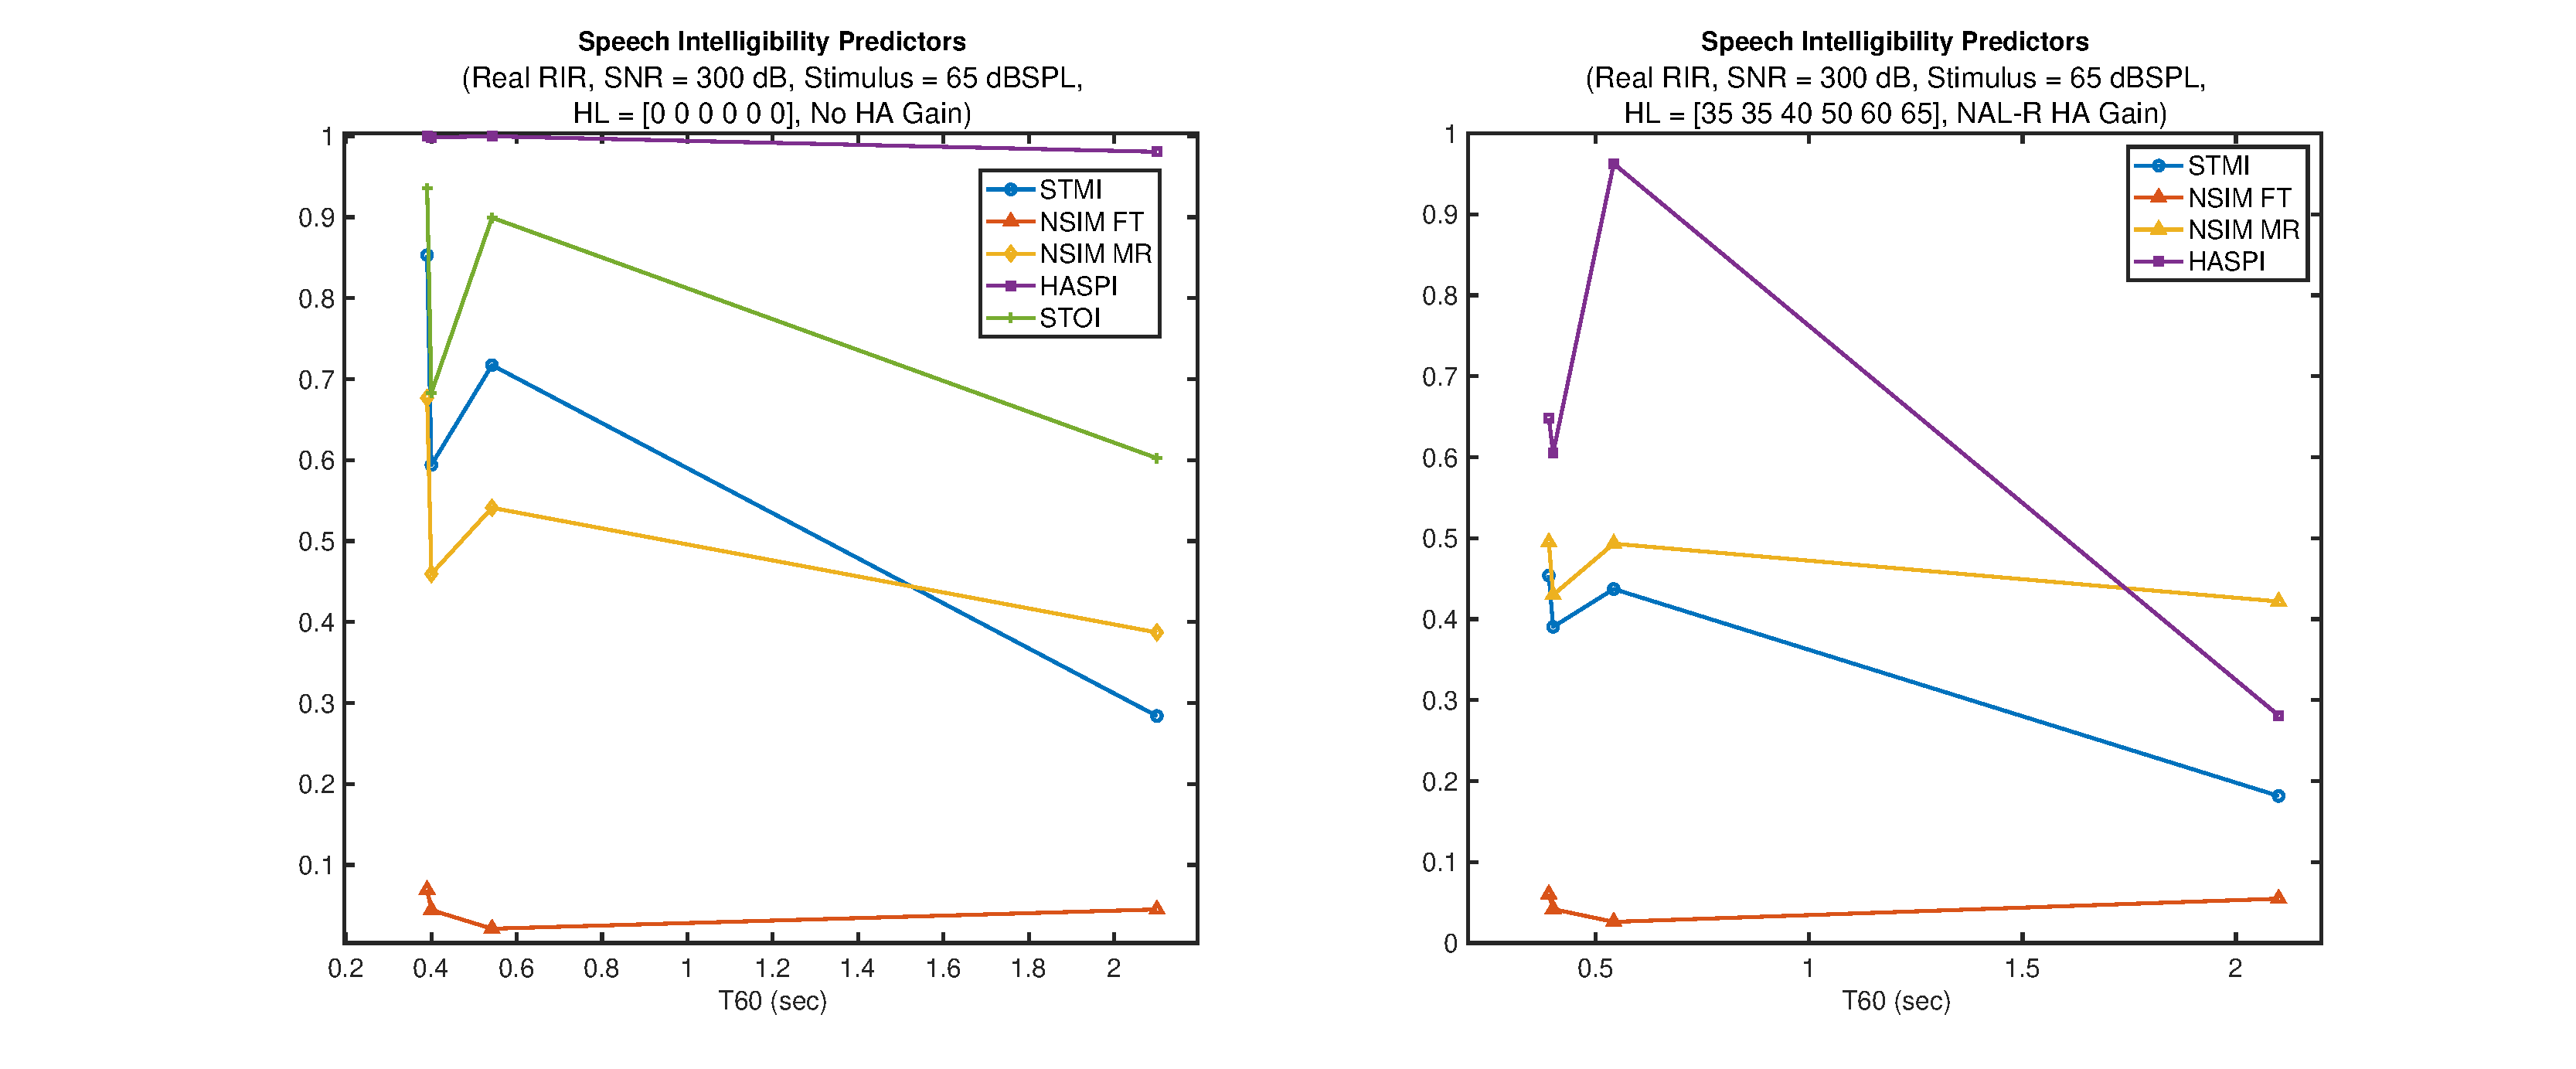
\includegraphics[width=0.98\textwidth]{SIMetricsEval_Real}
%	\centering
%	\caption{Impact of practical reverberation (several real measured RIRs) on SI predictors with and without hearing loss.}
%	\label{fig:SIMetricsEval_Real}
%\end{figure}

%\begin{figure}[H]
%	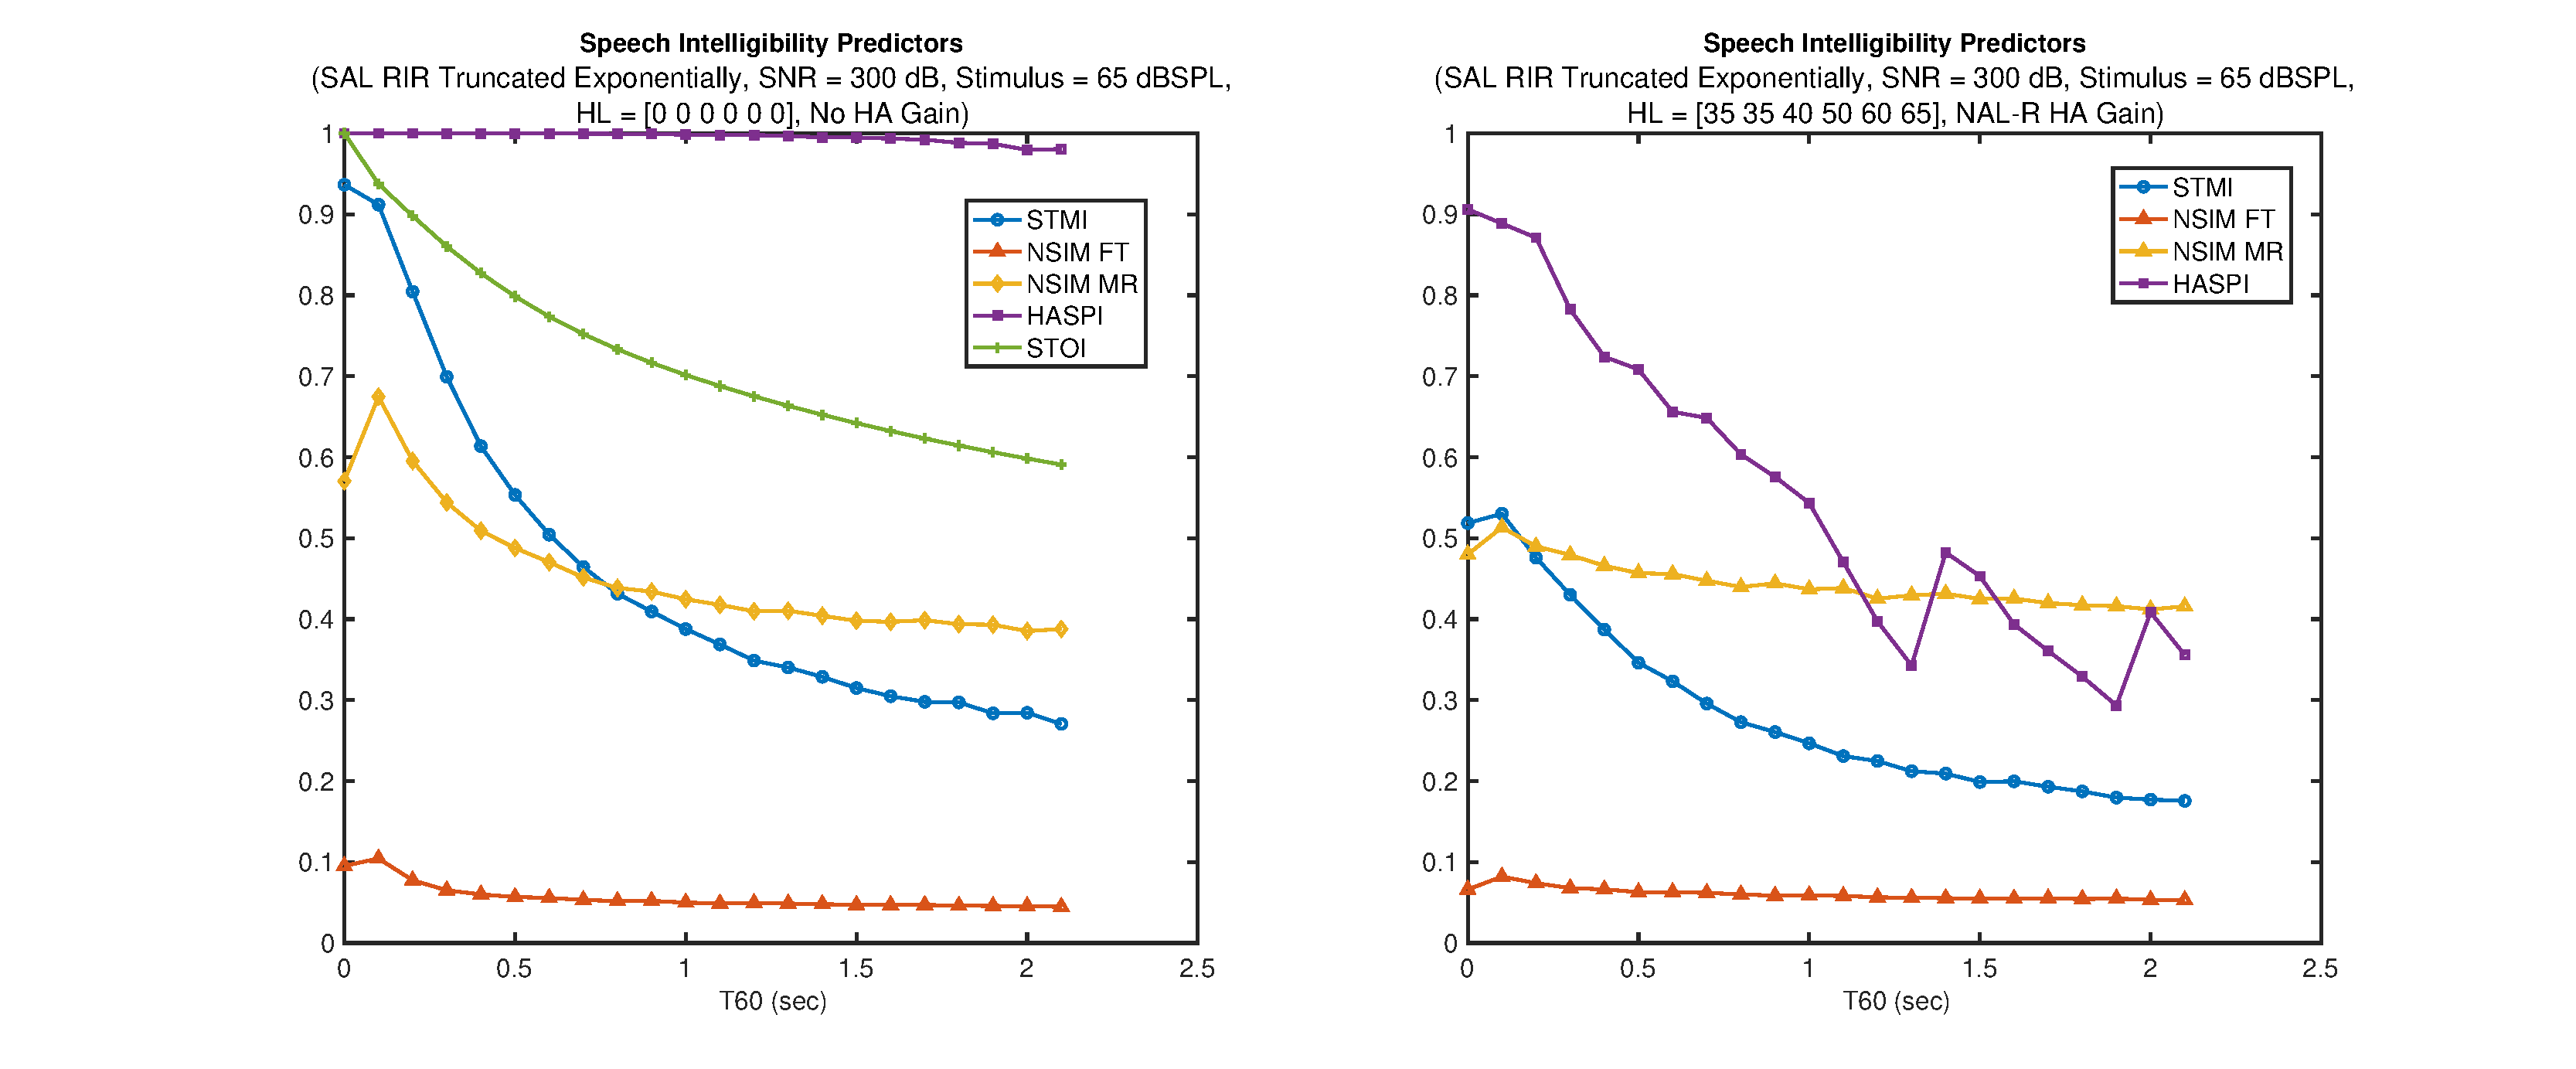
\includegraphics[width=0.98\textwidth]{SIMetricsEval_TruncatedSAL}
%	\centering
%	\caption{Impact of practical reverberation (SAL room from MYRiAD database exponentially truncated to control T60) on SI predictors with and without hearing loss. NAL-R linear hearing aid amplification included in hearing loss case for metrics that including modeling of hearing loss}
%	\label{fig:SIMetricsEval_TruncatedSAL}
%\end{figure}




%- Discussion of how T60 is not a complete picture of the effects of reverb, EDT and SI together provide a more complete description. Generally speaking these are both encapsulated collectively in DRR

%- Discussion of how NSIM and STMI continue to increase where HASPI plateaus suggesting that they can be used to reflect listening effort (NSIM and STMI still have some saturation, but not as much as subjective speech intelligibility). NSIM, STMI have no explicit application of a nonlinear  P/I function to map to SI, see notes about on how P/I function varies greatly depending on many factors so cant really be universal. The exact value of NSIM and STMI is not as meaningful, its moreso the how it changes with respect to control variables

%- HASPI is mapped to SI, but I dont think it has an explicity P/I function -- not clear need to investigate. It clearly does strongly saturate in a way the resembles subjective SI more accurately

%- Discussion of how NSIM and STMI were scaled (with a constant scaling factor accross all plots) to better view the trends accross all metrics on the same plot.



\section{Final Method Used} \label{section:final_method}

In this section, the method used for evaluating the perceptual benefit of delay-and-predict (DAP) dereverberation is outlined. Based on the analysis of the initial proposed method in Section \ref{section:initial_eval_method}, enhancements were made and the final evaluation method was defined.

The evaluation methodology was designed to allow three separate experiments:

\begin{enumerate}
	\item Evaluate the perceptual benefit of DAP dereverberation over a range of T60s using realistic reverberation
	%
	\item Evaluate the impact of realistic ambient noise on DAP performance
	%
	\item Evaluate the impact of a secondary talker in the same reverberant room on DAP performance
\end{enumerate}

Each experiment was conducted in two stages: a training phase and a evaluation phase. In the training phase (Figure \ref{fig:ThesisExperimentMethod_Training}), the DAP equalizer was blindly estimated from the reverberant microphone signals, corrupted by any interfering noise or secondary talker. In the evaluation phase (Figure \ref{fig:ThesisExperimentMethod_Eval}), the resulting DAP equalizer was applied to the reverberant microphone signals, without any noise or interfering talker, producing a dereverberated speech signal. The evaluation of the dereverberated signal in comparison to the reverberant microphone signal (i.e., before dereverberation) was done on the basis of SI/LE prediction to evaluate the perceptual benefit of the DAP equalizer. The noise/interfering talker were omitted from the evaluation phase to neglect the impact these interfering signals on SI/LE, and to focus only on their impact on dereverberation performance. Additionally, a different source signal was used in the training phase and evaluation phase to emphasize the potential that the ``over-whitening" of the training source signal may lead to an added reverberant effect when the equalizer is applied to a different signal (as described in Section \ref{section_dap}).

As explained in Section \ref{section:eval_si_metrics}, it was decided to simulate reverberation over a range of T60s by applying an exponentially decaying window function to the four-channel SAL RIR from the MYRiAD database (measured on a binaural pair of two-microphone BTE hearing aids), which has an initial T60 of \qty{2.2}{\sec}.

The RIRs were manually time-aligned, since time-of-flight estimation is a well understood field in signal processing and was left outside of the scope of this experiment. Additionally, all RIR measurement noise leading to the direct sound impulse was manually removed using a fixed magnitude threshold to avoid unrealistic convolution of these noise samples with the source signals as described in Section \ref{section:params_p2_MC_LP}

The source speech signal used accross all experiments, was \qty{10}{\sec} of speech generated by concatenating multiple different utterance samples of the same male talker from the TMIT speech sample database \citep{garofolo1993timit}. A \qty{10}{\sec} duration speech stimulus was selected as per discussion in DAP parameter tuning conclusions in Section \ref{section:params_conclusion}. The speech signal was calibrated to a conversational speech level of \qty{65}{\decibel SPL}. This calibration was done based on the convolution of the the source speech signal with the the direct sound / early reflections from the RIR (i.e., the first \qty{50}{\milli\sec}), since this is the perceived speech level due to the temporal integration of early reflections. The source signal was then convolved with the full exponentially windowed RIR and added with the interfering noise / secondary talker.

To generate realistic ambient noise, the multichannel noise recordings from the HRIR database were used. Two separate noise recordings were included in the evaluation: a ventillation noise recording from the ``office" room (approximately stationary), and a babble noise recording from the ``cafeteria" room (highly non-stationary). The average RMS level accross the four channels was then calibrated to achieve the desired SNR before adding with the reverberant speech signal above.

To generate a realistic secondary talker in the same room, a separate \qty{10}{\sec} speech stimulus from the TMIT database was convolved with a different four-channel RIR measurement corresponding to another location in the the SAL room in the MYRiAD database. This four-channel RIR was also exponentially windowed to the same T60. The target talker was placed in front of the head-and-torso simulator (\qty{0}{\degree}) and the interfering talker was placed to the side (\qty{90}{\degree}). After convolving the interfering talker source signal with the corresponding four-channel RIR, the resulting reverberant signals were level-calibrated to the desired signal-to-interference ratio (SIR) before adding with the target reverberant speech signal above.

The resulting four-channel simulated microphone signals, $\boldsymbol{y}(n)$, were then used as input to the DAP algorithm, producing the DAP equalizer, $\boldsymbol{H}(z)$. As per the DAP parameter tuning conclusions in Section \ref{section:params_conclusion}, the MC-LP prediction order was initially set to $p_2=\left(\mathrm{T60}_{\mathrm{max}} \cdot f_s \right)/\left(M-1\right)$, with a sample rate of $f_s = \qty{16}{\kilo\hertz}$, $\mathrm{T60}_{\mathrm{max}} = \qty{1}{\sec}$ and $M=4$. The source-whitening prediction order was set to $p_1 = 1.25 \cdot p_2 \cdot \left(M-1\right)$. This resulted in prediction orders of $p_2 = 5333$ and $p_1 = 20000$.

In the evaluation phase (Figure \ref{fig:ThesisExperimentMethod_Eval}), the first channel of the reverberant microphone signals ($y_1(n)$ from $\boldsymbol{y}(n)$) and the dereverberated DAP output signal ($\hat{s}(n)$) were both analyzed for SI/LE. The analysis of SI/LE was done for each case by comparing the test signal to a clean source reference signal, producing STOI, HASPI, FT-NSIM, MR-NSIM and STMI. Like in Section \ref{section:eval_si_metrics}, these metrics were scaled such that a value of 1.0 is acheived for the signal obtained by the convolution of the source signal with just the direct sound and early reflections of the RIR. Additionally, VISQOL and HASQI were produced to evaluate speech quality (SQ). Lastly, clarity (C50) was computed to provide a physical reveberation-specific metric. Metrics that include perceptual models of hearing loss were additionally re-computed with a standard moderate high-frequency hearing loss profile was used \citep[IEC 60118-15 moderate hearing loss, moderately sloping group, ][]{bisgaard2010standard}, and a NAL-R linear hearing aid gain vector was applied.

To show the impact of any stochasticity in the test conditions and auditory models, all experiments in this chapter were repeated 10 times and plotted with error bars showing standard deviation.


%\begin{sidewaysfigure}[H]
%	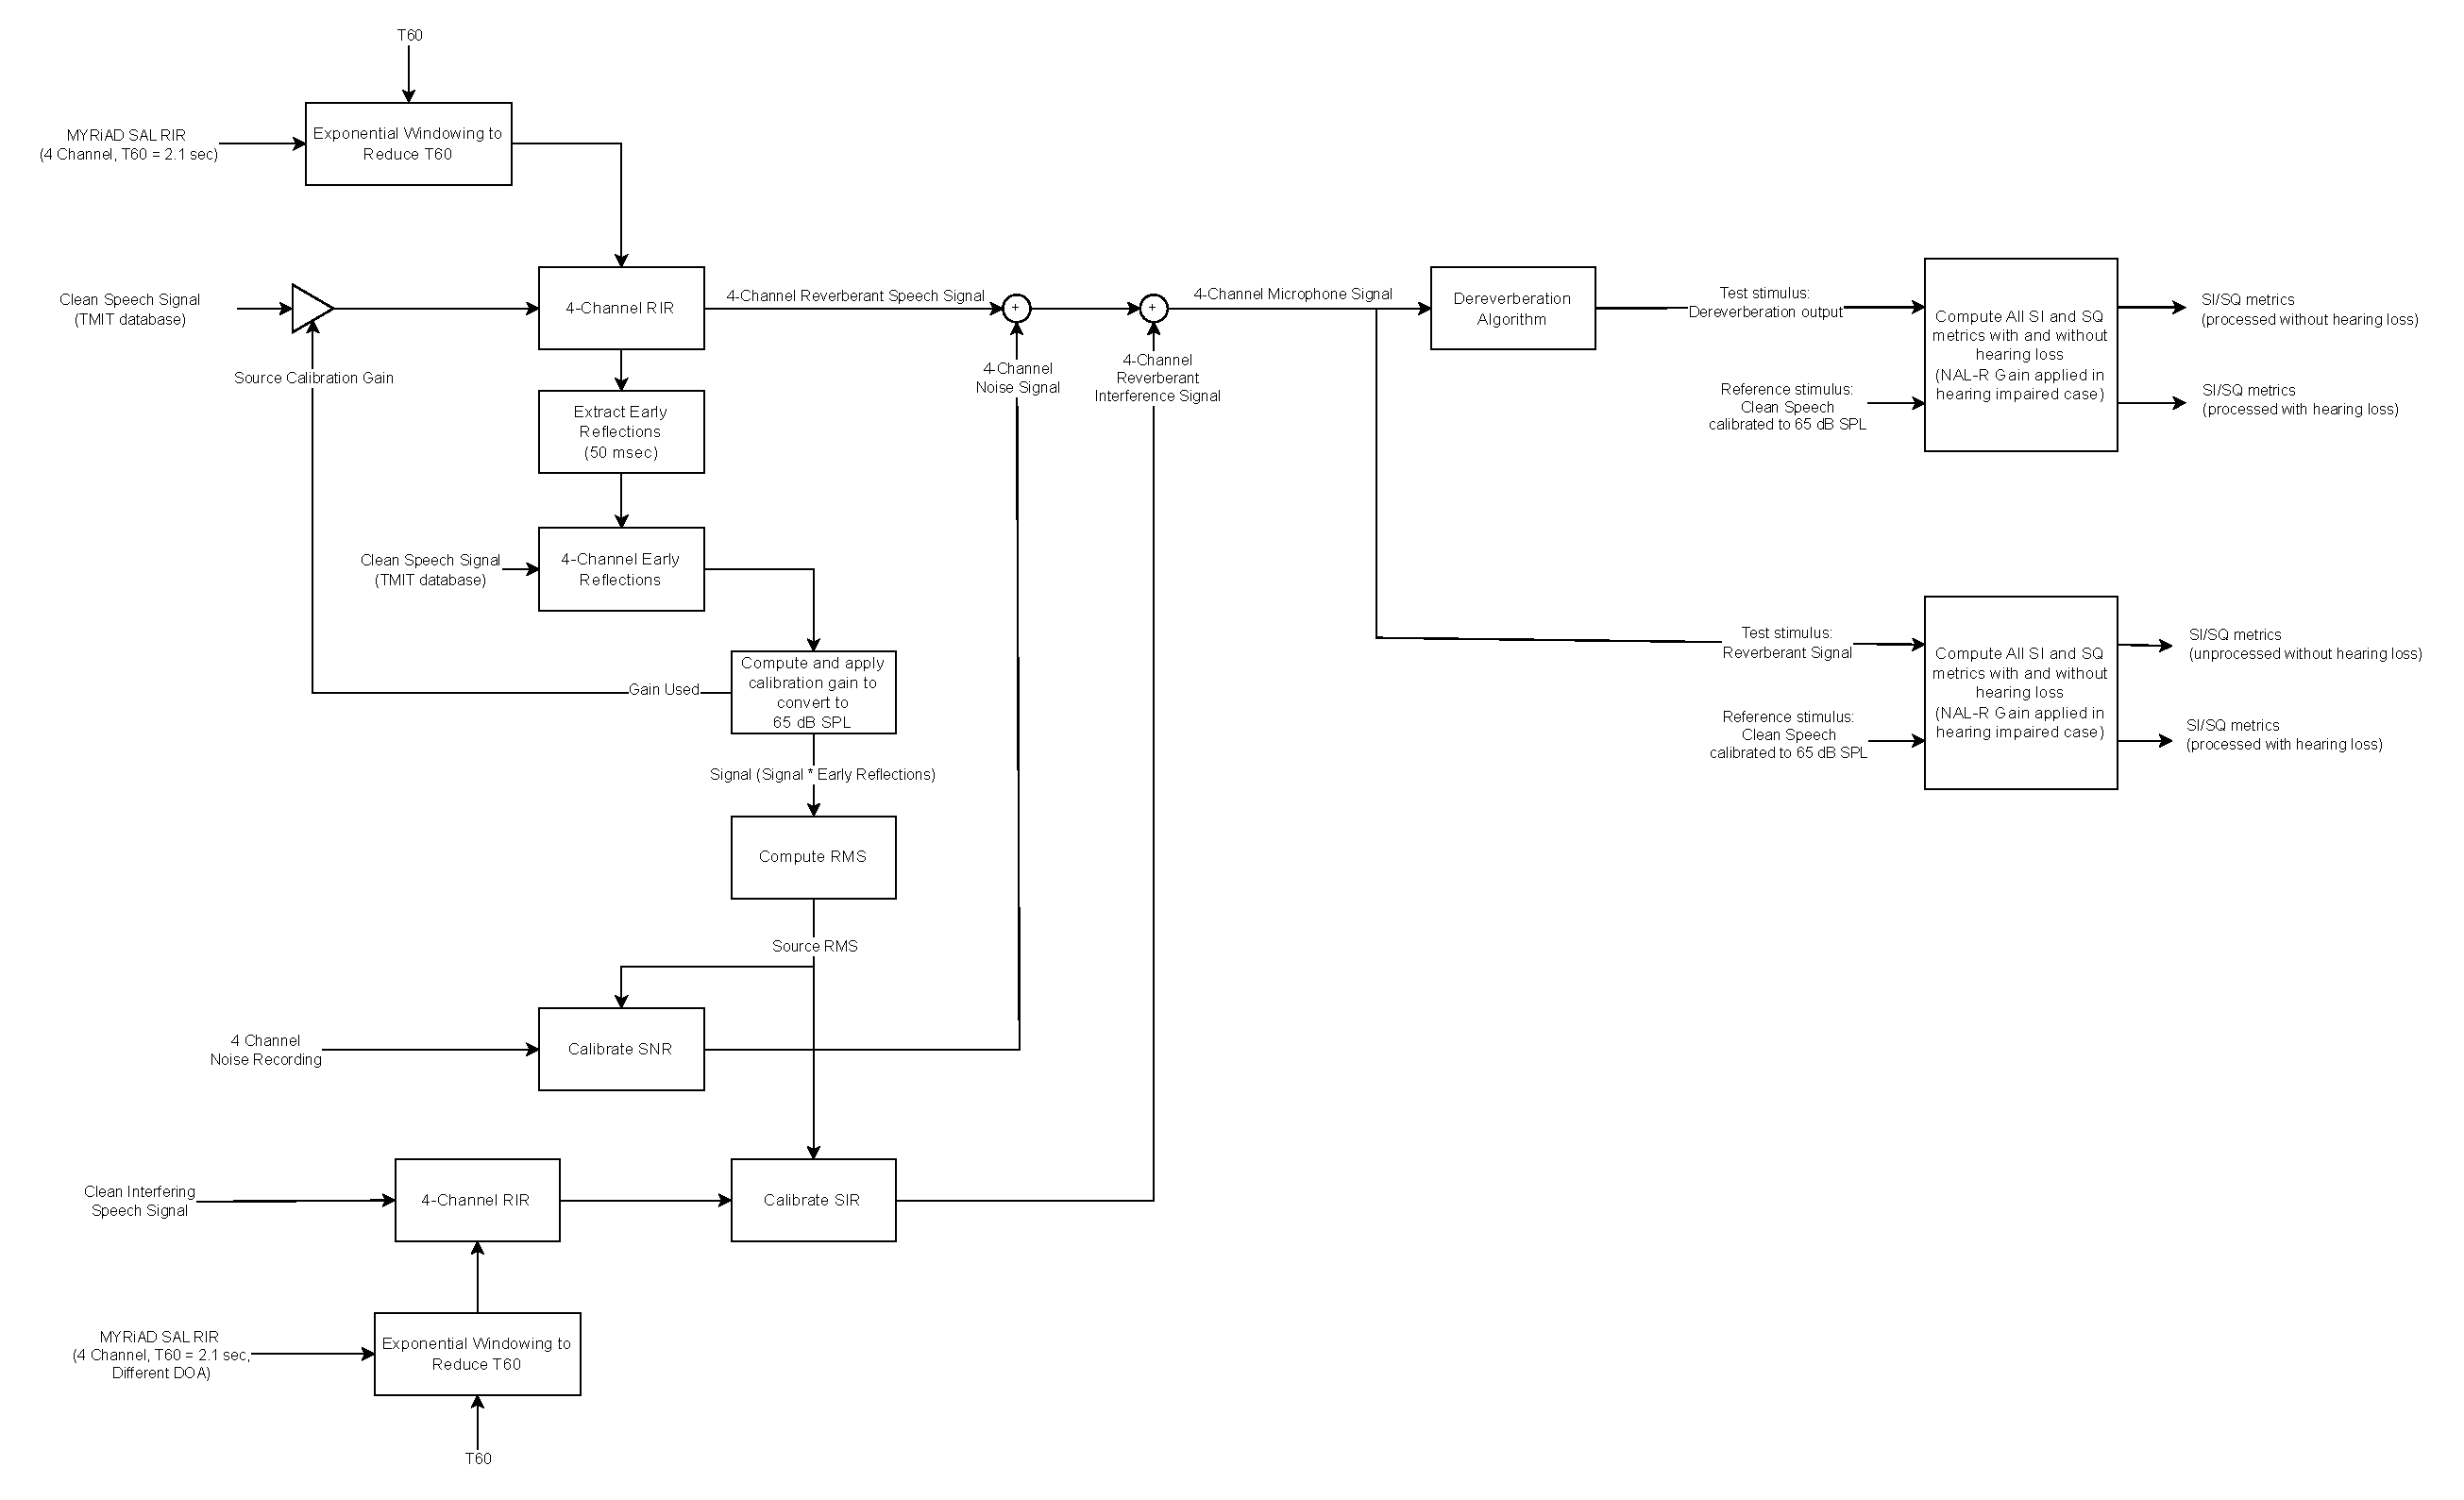
\includegraphics[height=0.9\textheight]{ThesisExperimentMethod}
%	\centering
%	\caption{Block diagram for method used in evaluating dereverberation algorithm performance. Microphone signals include reverberant speech (MYRiAD SAL RIR windowed exponentially to control T60) with added noise signal (real multichannel noise recordings) and added reverberant interference signal. All SI and SQ predictors were computed for the unprocessed microphone signals and the dereverberation output both with and without hearing loss included in all models of speech perception.}
%	\label{fig:Evaluation_Block_Diagram}
%\end{sidewaysfigure}

\newpage
\vfill

\begin{sidewaysfigure}
	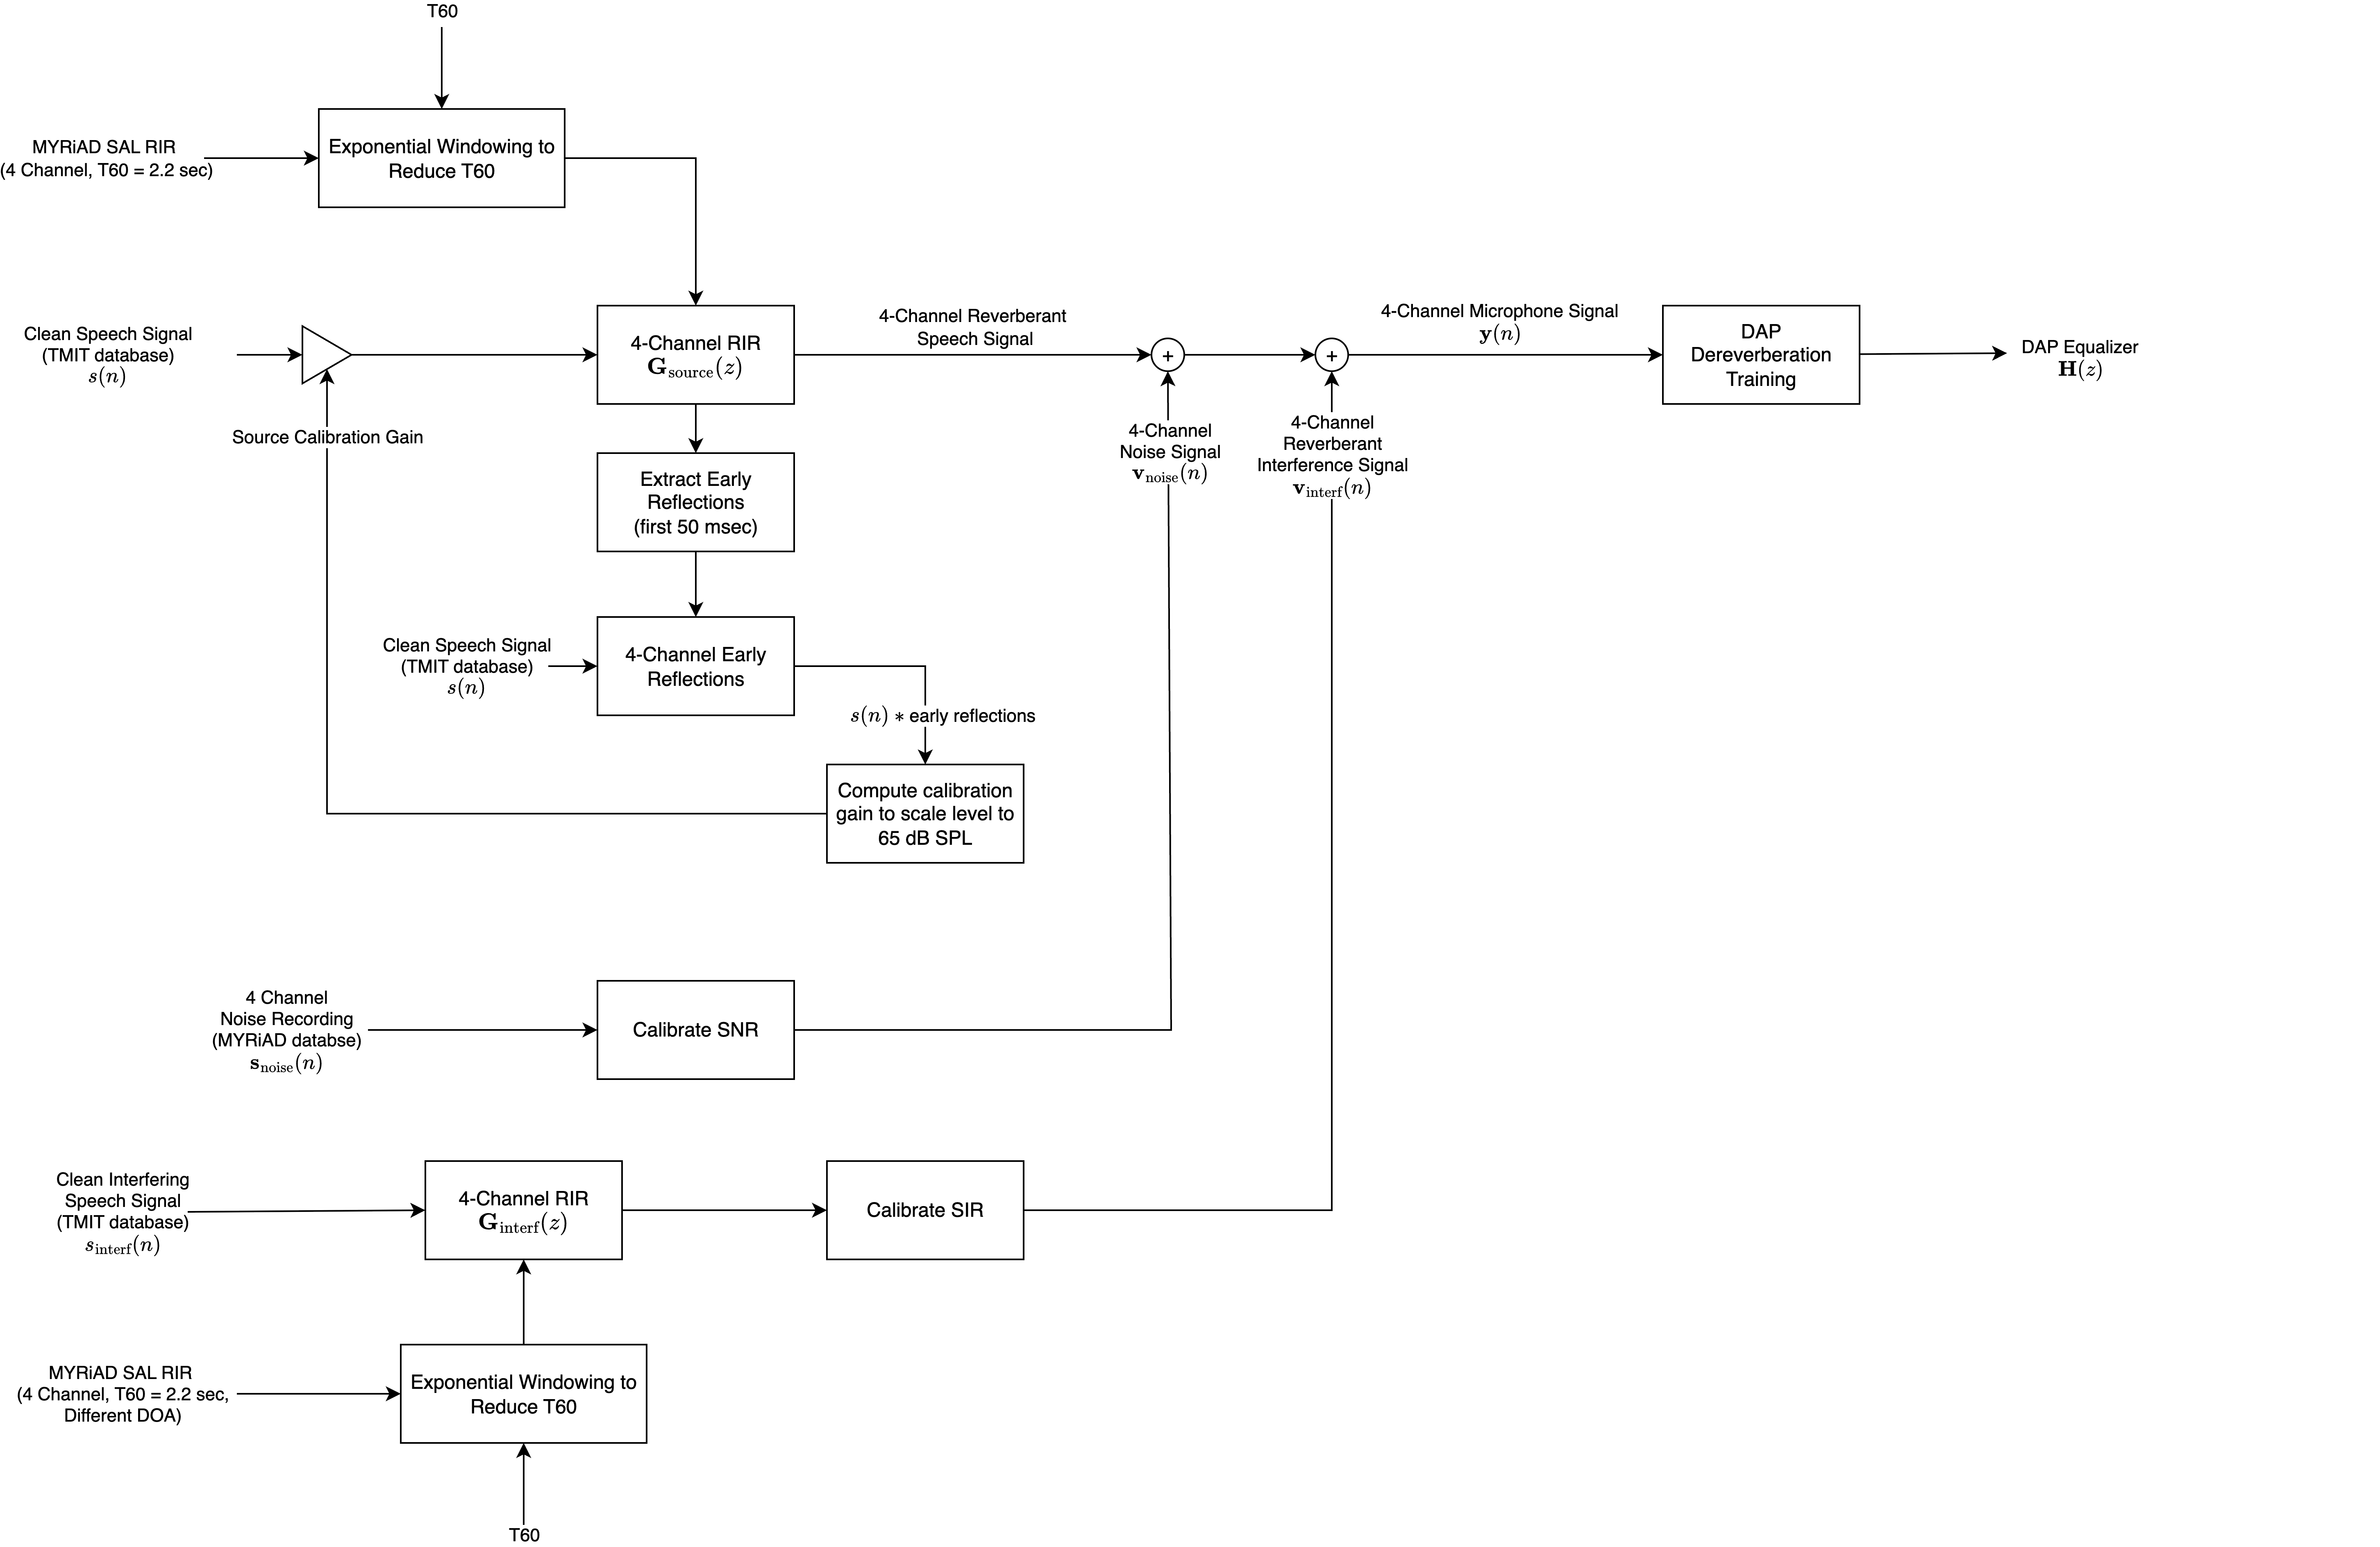
\includegraphics[width=\columnwidth]{ThesisExperimentMethod_Training}%
	\caption[Block diagram for training phase of the final evaluation method]{Block diagram for the training phase of the method used in evaluating dereverberation algorithm performance. Microphone signals include reverberant speech (MYRiAD SAL RIR windowed exponentially to control T60) with added noise signal (real multichannel noise recordings) and added reverberant interference signal. The output of the training phase is the DAP equalizer which is used in the evaluation phase (Figure \ref{fig:ThesisExperimentMethod_Eval}).}
	\label{fig:ThesisExperimentMethod_Training}
\end{sidewaysfigure}

\vfill
\clearpage

\newpage
\vfill

\begin{sidewaysfigure}
	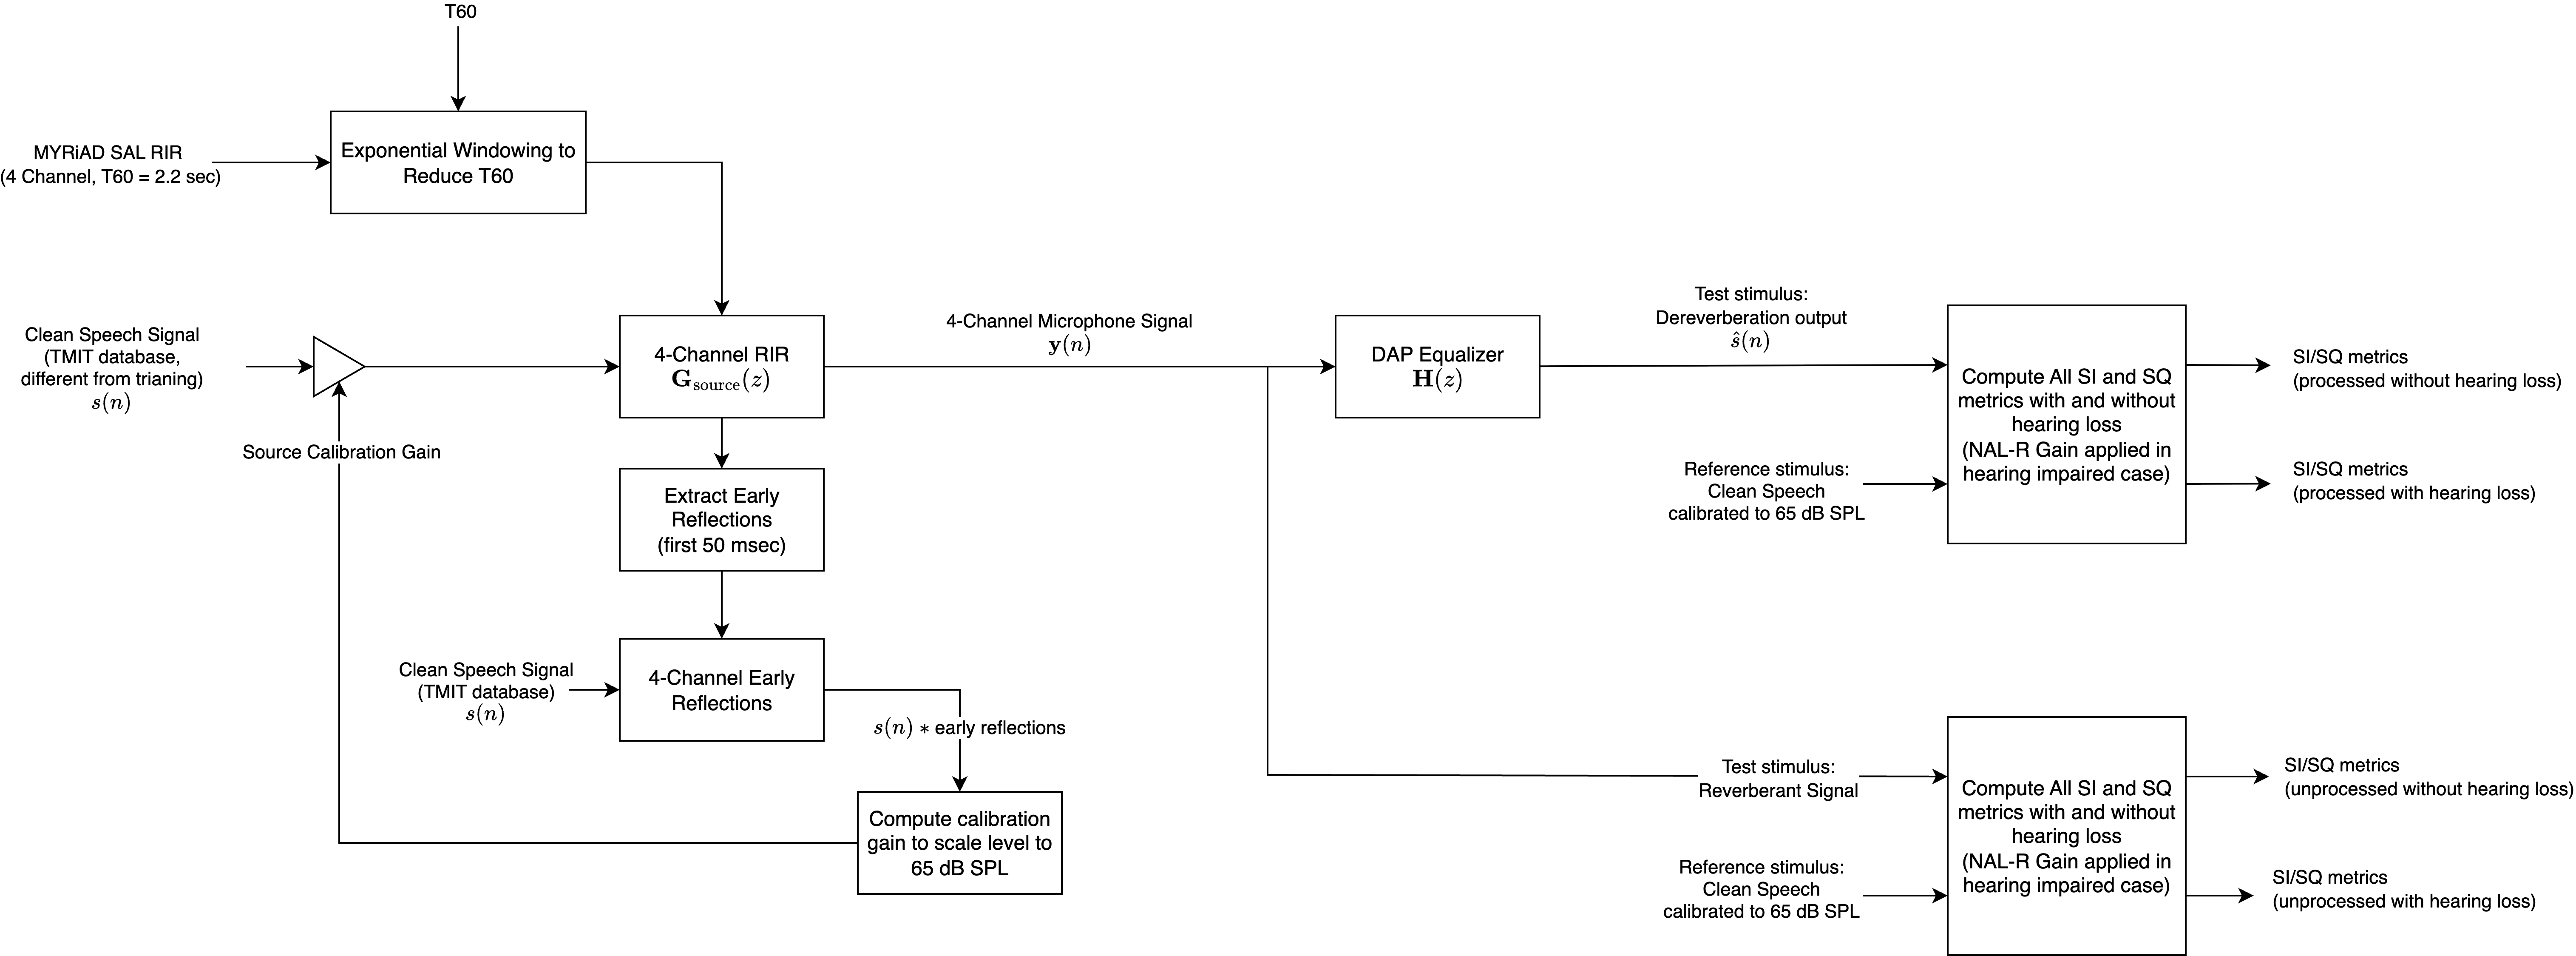
\includegraphics[width=\columnwidth]{ThesisExperimentMethod_Eval}%
	\caption[Block diagram for evaluation phase of the final evaluation method]{Block diagram for the evaluation phase of the method used in evaluating dereverberation algorithm performance. Microphone signals include reverberant speech (MYRiAD SAL RIR windowed exponentially to control T60). Noise and Interfering speech were omitted during evaluation to focus on dereverberation performance only. A different source signal from the training phase was purposefully used. All SI and SQ predictors were computed for the unprocessed microphone signals and the dereverberation output both with and without hearing loss included in all models of speech perception. Additionally, clarity ($\mathrm{C50}$) was computed from the resulting EIR.}
	\label{fig:ThesisExperimentMethod_Eval}
\end{sidewaysfigure}

\vfill
\clearpage




%\section{Delay-and-Predict Dereverberation Evaluation with Synthetic Reverberation}

%\textbf{TODO: Redo all eval plots with regularization added. Already run on server ($\text{FINAL}\_\text{RESULTS}\_\text{wReg}$) just need to format and input figures to thesis}

%\textbf{SI/SQ/Clarity v T60 w/ no noise}

%\begin{figure}[H]
%	\centering
%	\begin{subfigure}[b]{0.47\textwidth}
%		\centering
%		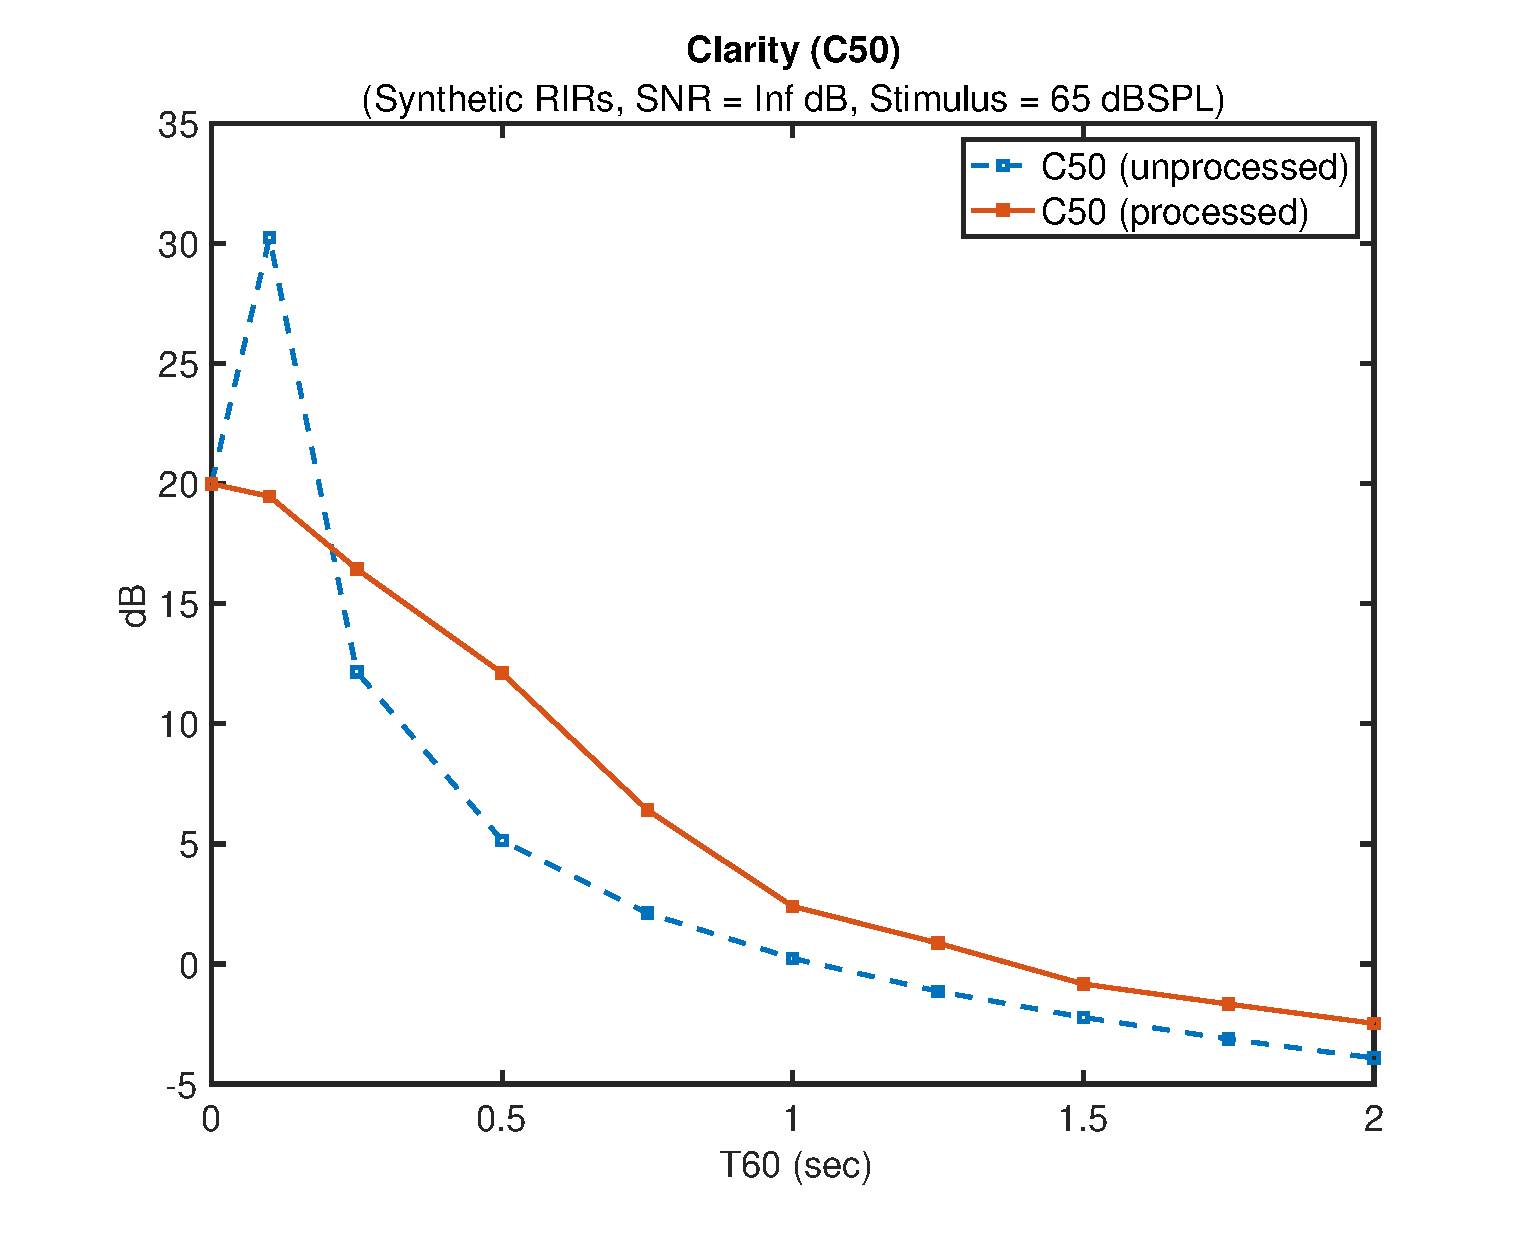
\includegraphics[width=\textwidth]{DAP_EvalT60Sweep_Synthetic_NoNoise_C50_v_T60}
%	\end{subfigure}
%	\begin{subfigure}[b]{0.92\textwidth}
%		\centering
%		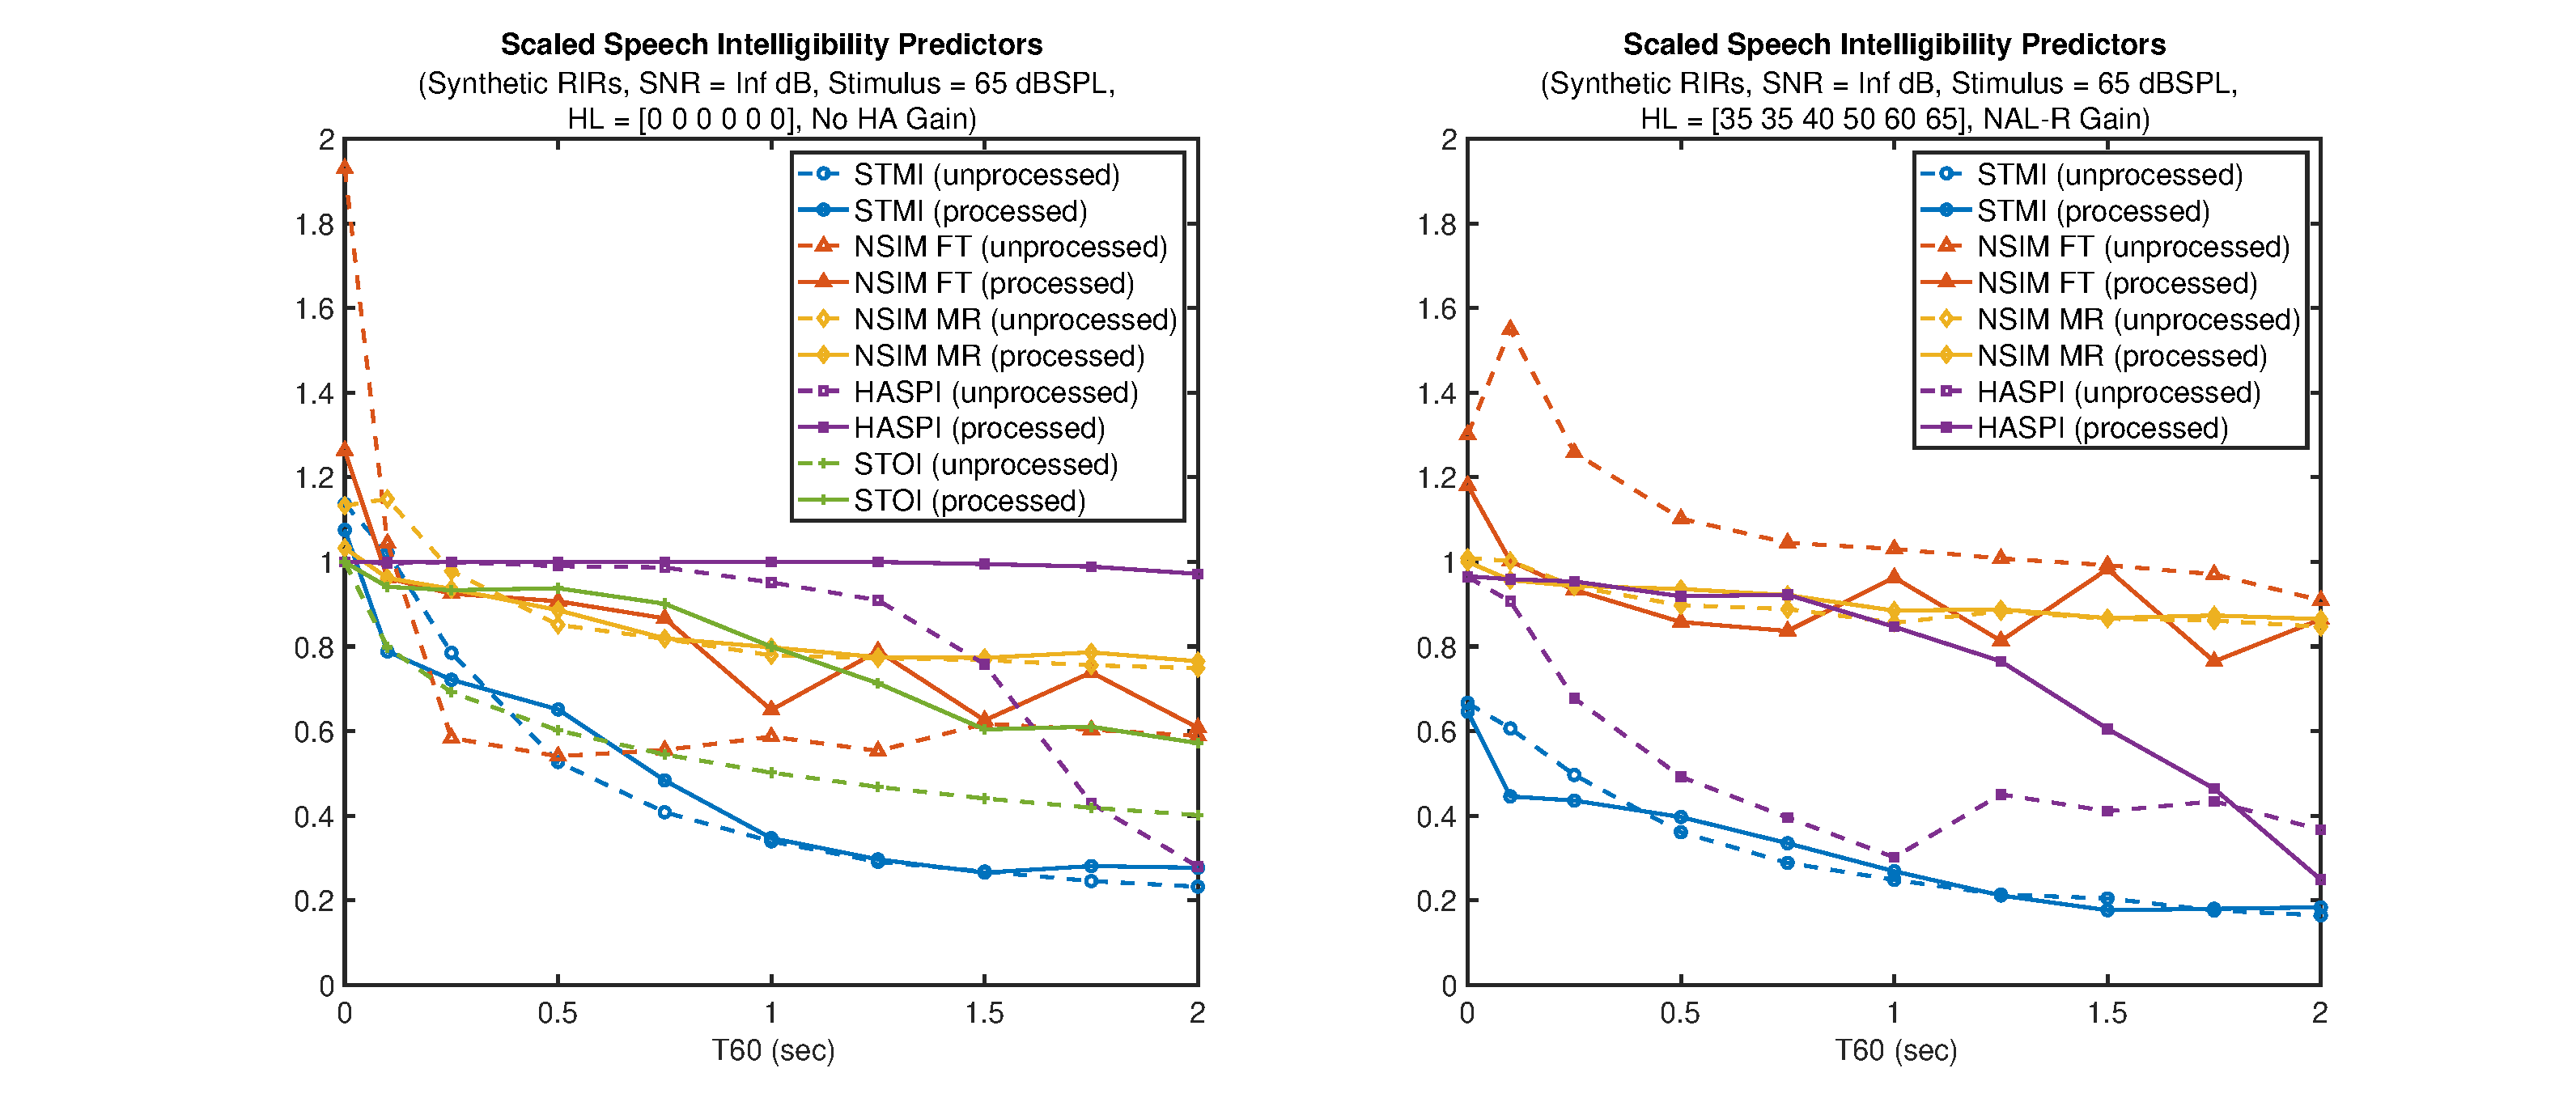
\includegraphics[width=\textwidth]{DAP_EvalT60Sweep_Synthetic_NoNoise_SI_v_T60}
%	\end{subfigure}
%	\begin{subfigure}[b]{0.92\textwidth}
%		\centering
%		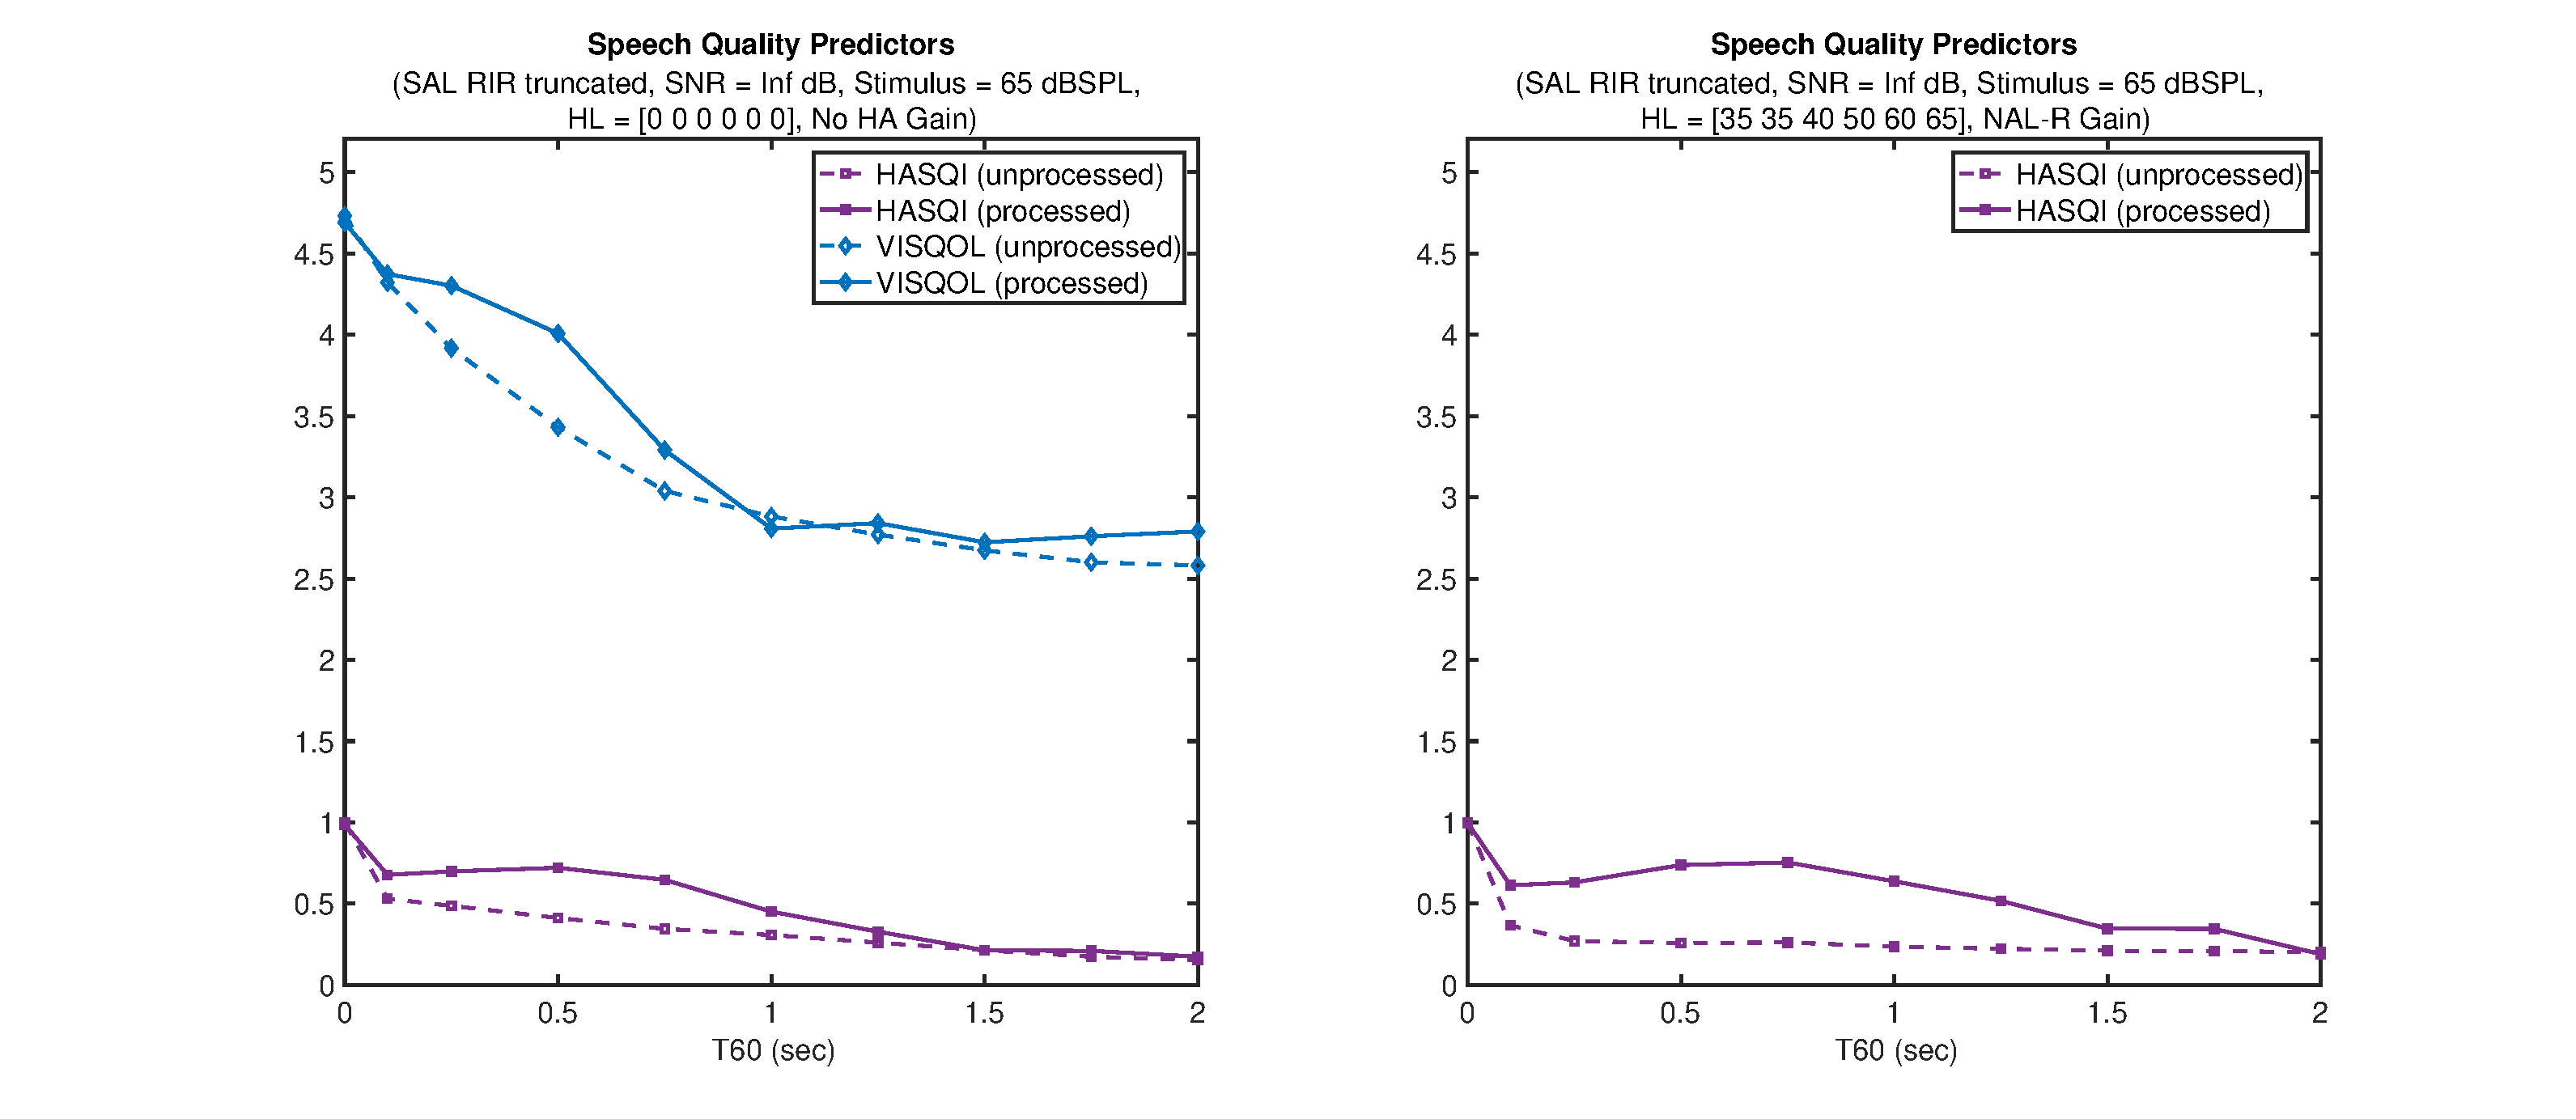
\includegraphics[width=\textwidth]{DAP_EvalT60Sweep_Synthetic_NoNoise_SQ_v_T60}
%	\end{subfigure}
%	\caption{Evaluation of delay-and-predict dereverberation performance as a function of T60. RIRs were synthetically generated by applying a variable decay-rate exponential window to sequences of uncorrelated Gaussian white noise.}
%	\label{fig:DAP_EvalT60Sweep_Synthetic_NoNoise}
%\end{figure}

%\begin{figure}[H]
%	\centering
%	\begin{subfigure}[b]{0.47\textwidth}
%		\centering
%		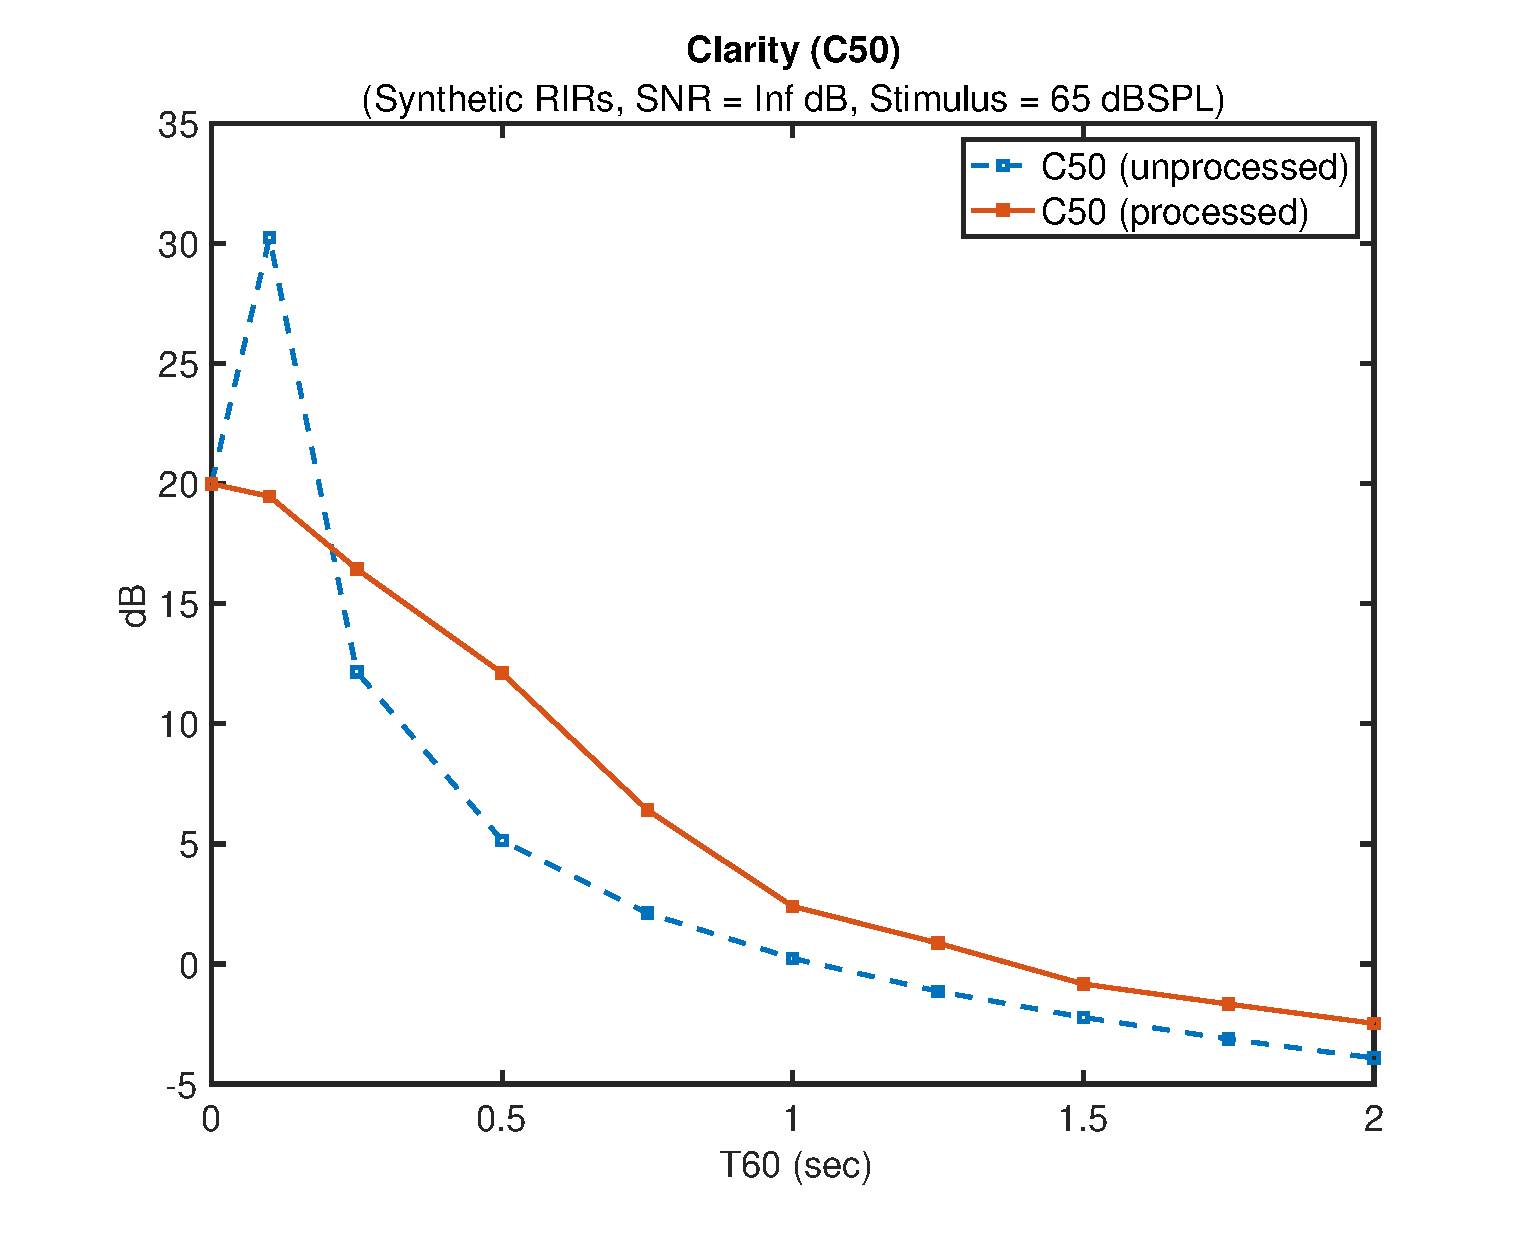
\includegraphics[width=\textwidth]{DAP_EvalT60Sweep_Synthetic_NoNoise_C50_v_T60}
%	\end{subfigure}
%	\begin{subfigure}[b]{0.92\textwidth}
%		\centering
%		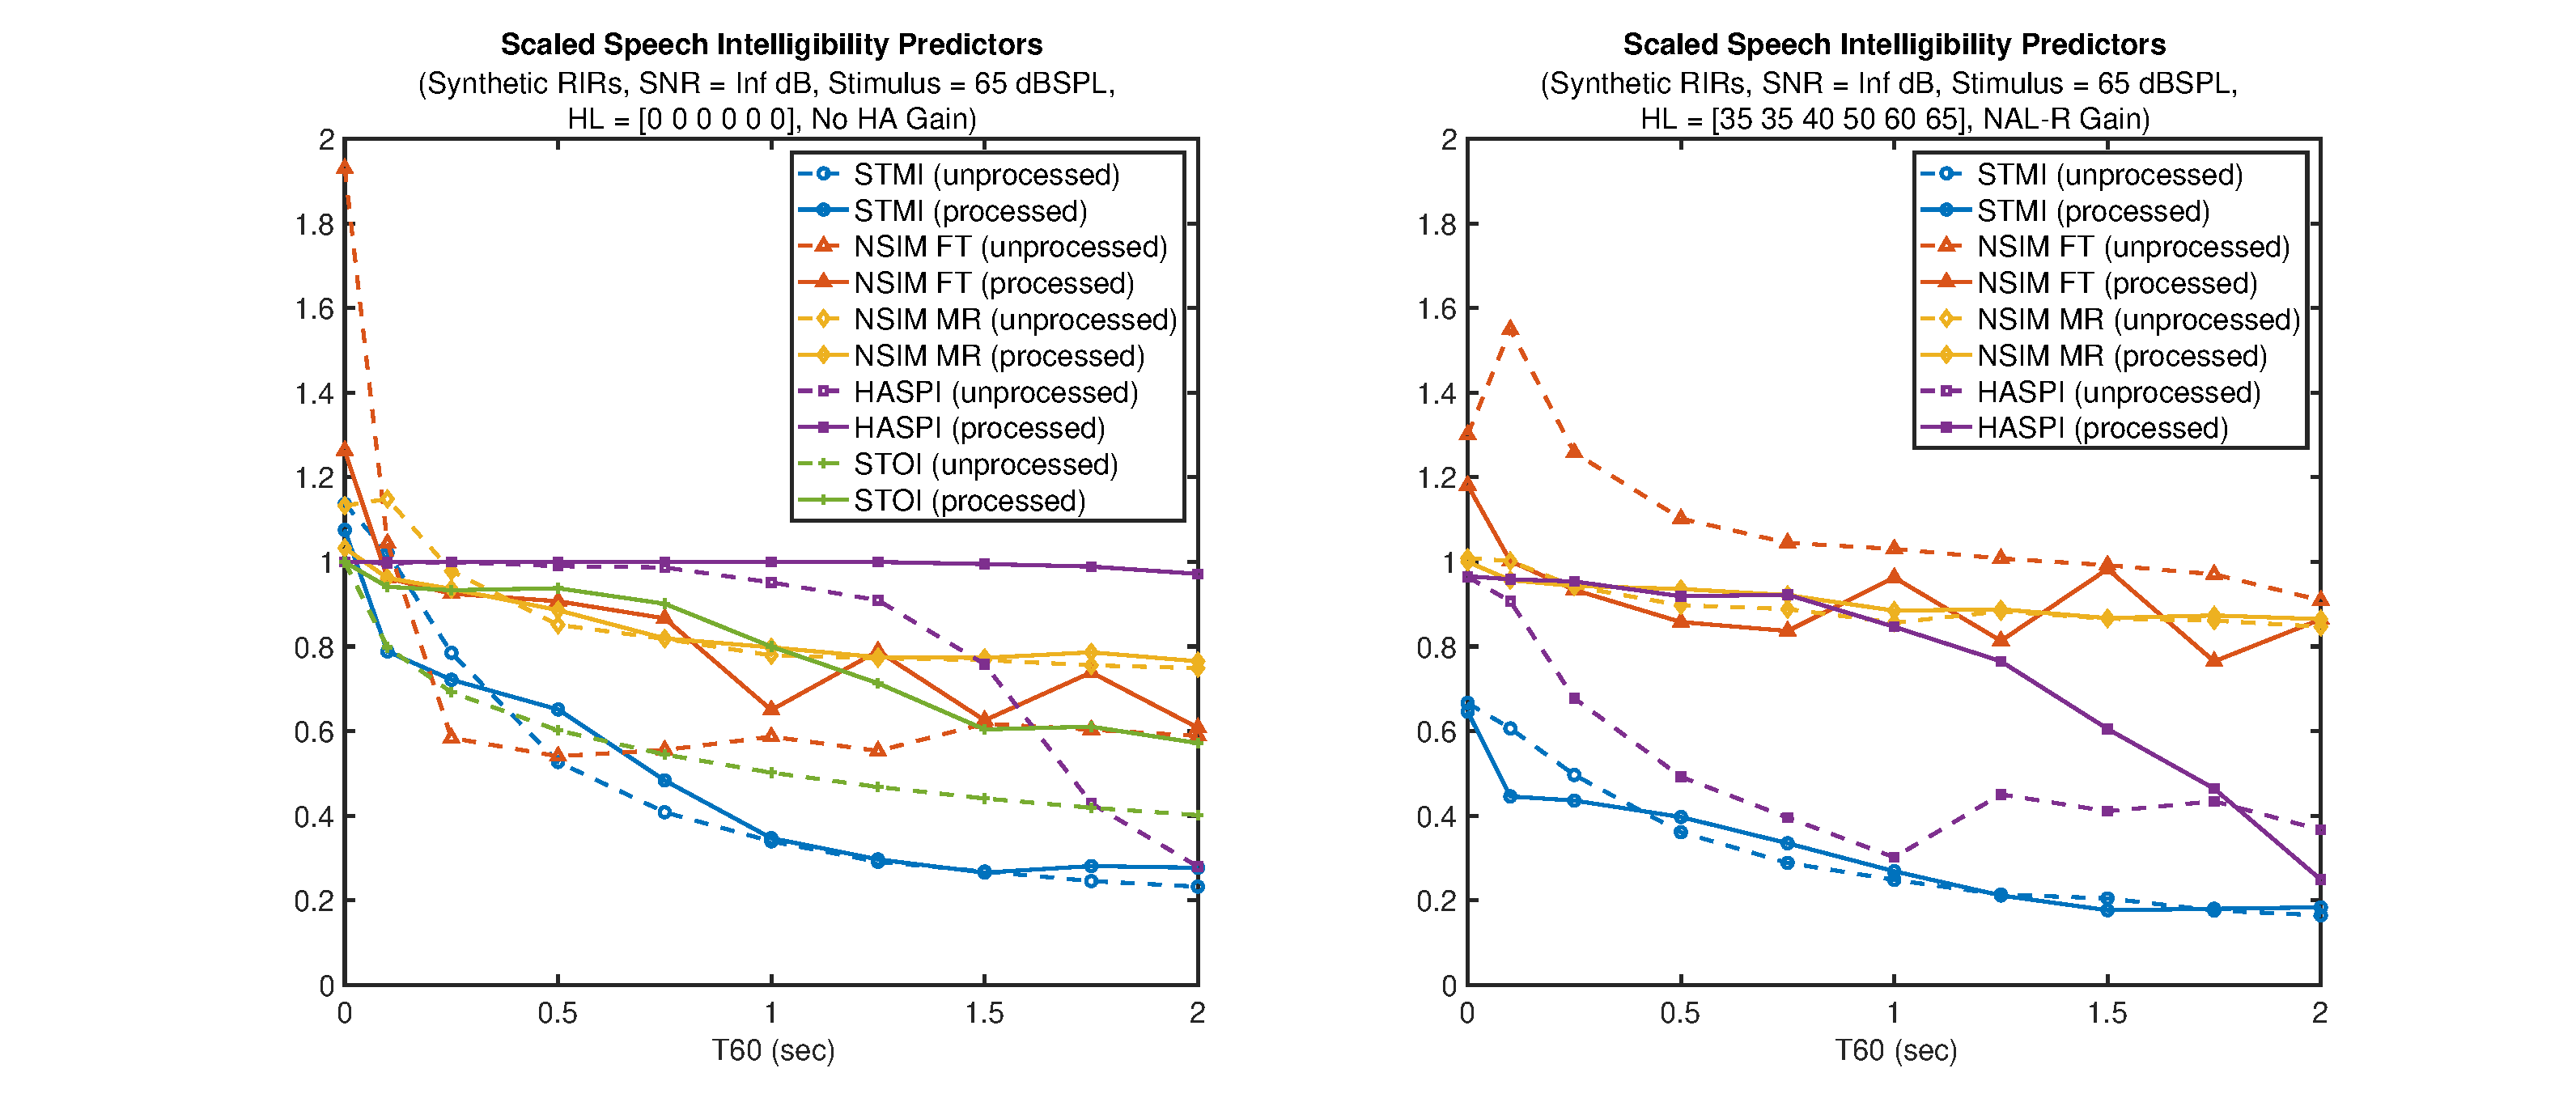
\includegraphics[width=\textwidth]{DAP_EvalT60Sweep_Synthetic_NoNoise_SI_v_T60}
%	\end{subfigure}
%	\begin{subfigure}[b]{0.92\textwidth}
%		\centering
%		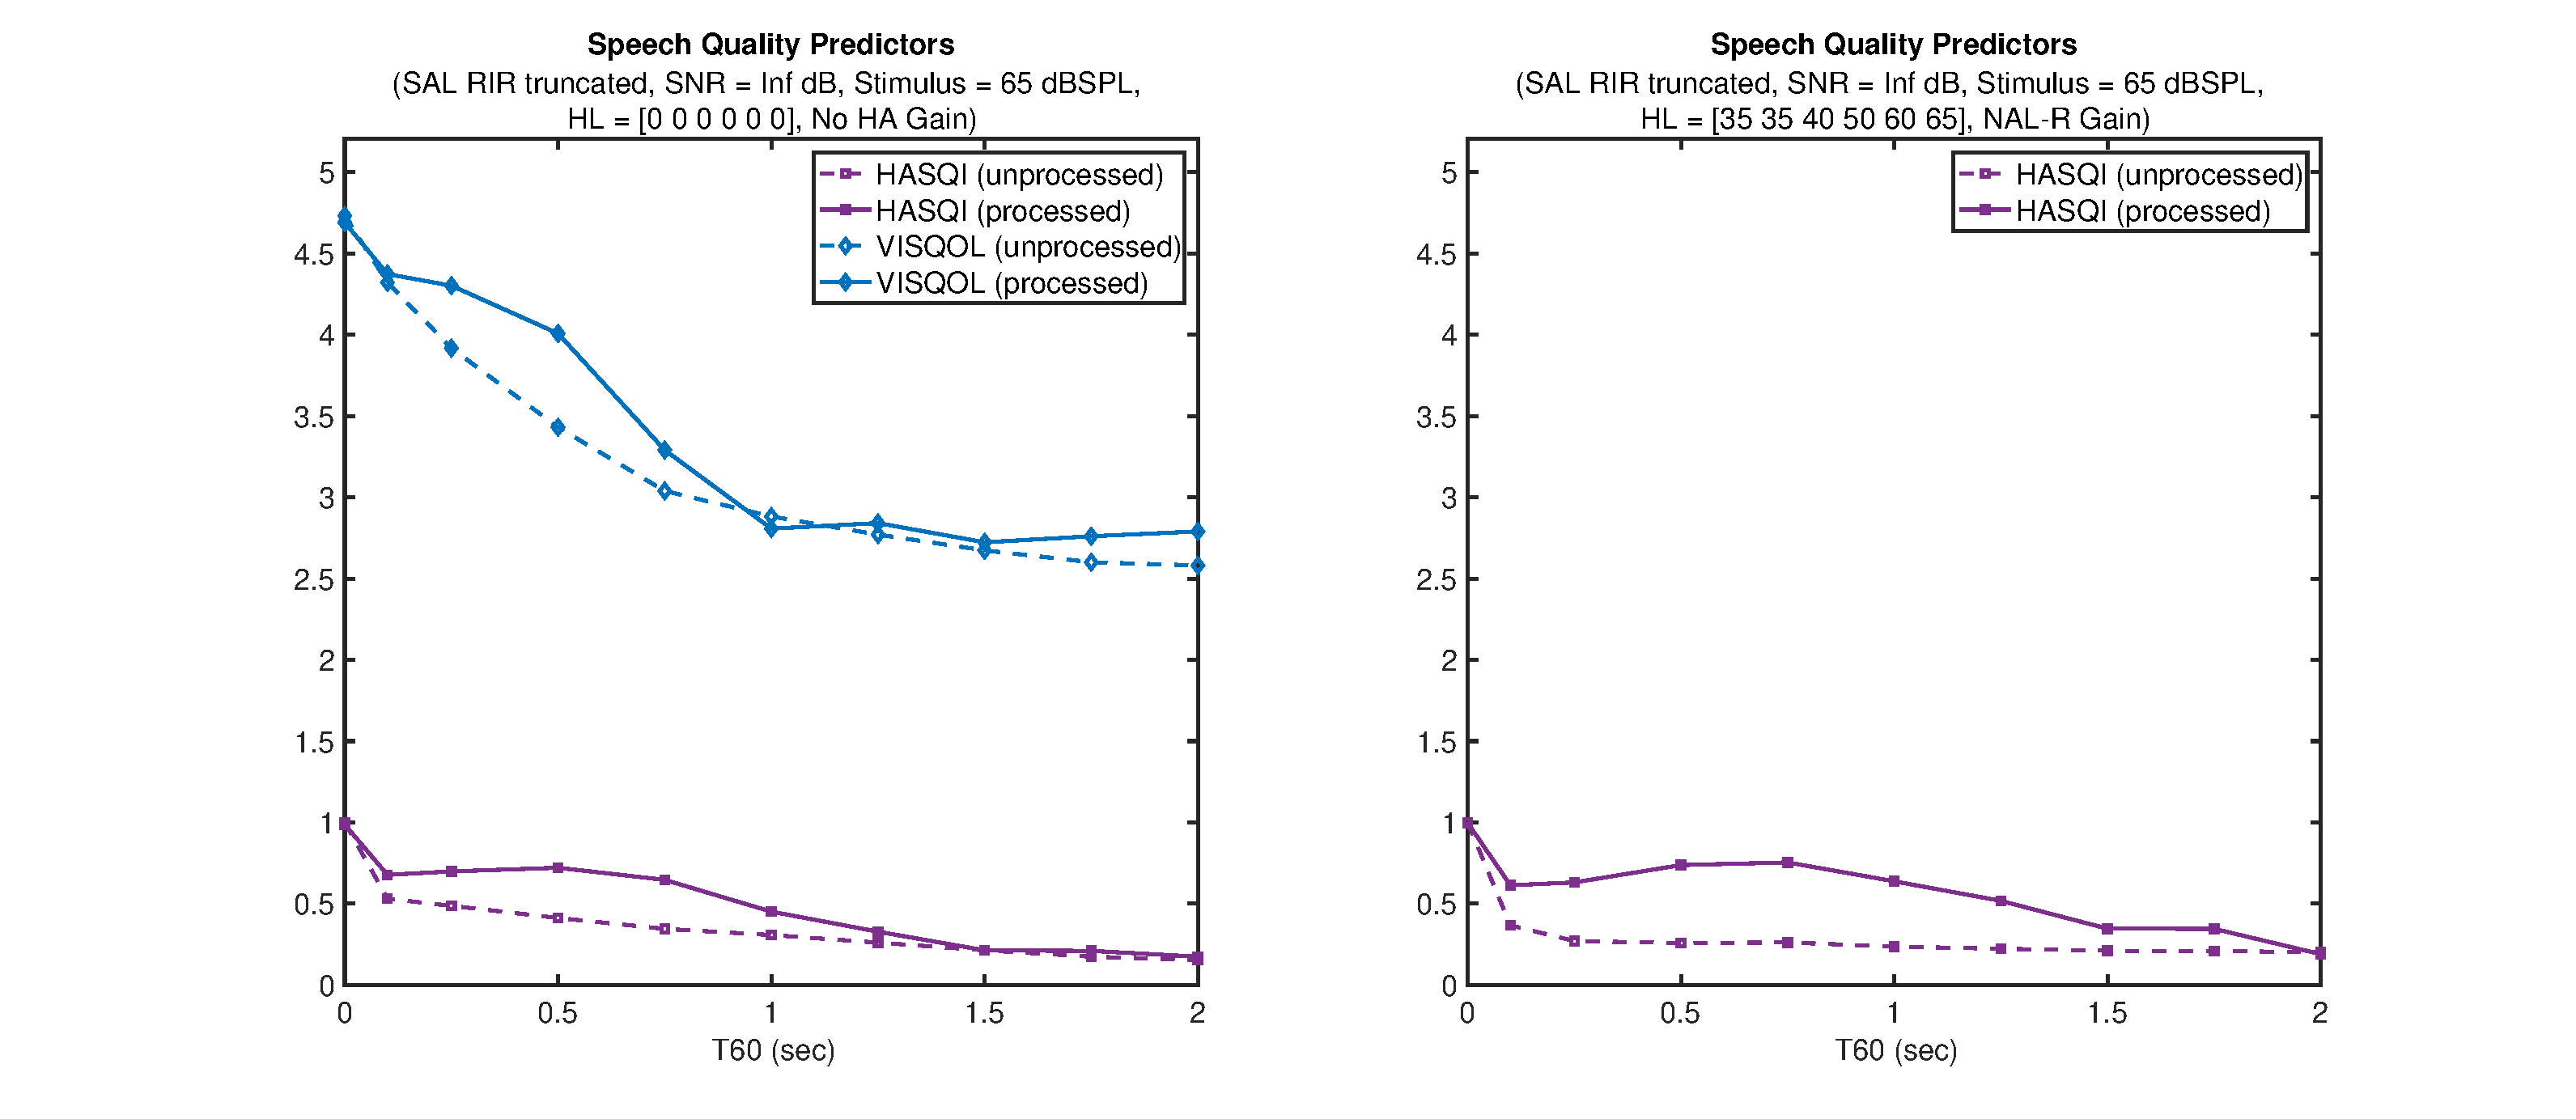
\includegraphics[width=\textwidth]{DAP_EvalT60Sweep_Synthetic_NoNoise_SQ_v_T60}
%	\end{subfigure}
%	\caption{Evaluation of delay-and-predict dereverberation performance as a function of T60. A small regularization factor was added to the average autocorrelation matrix and multi-channel spatio-temporal correlation matrix used in the normal equations for stages 1 and 2 respectively \textbf{TODO}. RIRs were synthetically generated by applying a variable decay-rate exponential window to sequences of uncorrelated Gaussian white noise.}
%	\label{fig:DAP_wReg_EvalT60Sweep_Synthetic_NoNoise}
%\end{figure}


\section{Delay-and-Predict Dereverberation Evaluation in Variable Reverberation} \label{section:dap_eval_truncSAL}

In this section, DAP dereverberation performance was evaluated over various amounts of reverberation by manipulating the T60 of the MYRiAD SAL RIR using the method described Section \ref{section:final_method}. Using the algorithm training/evaluation methods described in Figure \ref{fig:ThesisExperimentMethod_Training} and Figure \ref{fig:ThesisExperimentMethod_Eval}, all objective predictors of SI (STOI, HASPI, FT-NSIM, MR-NSIM and STMI), all objective predictors of SQ (VISQOL, HASQI) and C50 were generated at each T60 for both the unprocessed reverberant signal and the dereverberated output of the DAP algorithm. Metrics before and after DAP processing were plotted over T60s. The results for this initial evaluation with and without hearing loss included are shown in Figure \ref{fig:DAP_EVAL_1000T60max_noReg}.

%For this initial evaluation, the DAP prediction orders were set to optimally cancel up to a T60 of \qty{1}{\sec} as discussed in Section \ref{section:params_conclusion} (i.e., $p_2 = 5333$ and $p_1=20000$)
	
%The experiment was repeated with hearing loss included in models which support this. As previously discussed, a standard high-frequency hearing loss profile was used (IEC 60118-15 Moderate HL, Moderately Sloping Group), and NAL-R linear hearing aid gain was applied.

%In the calculation of the FT-NSIM and MR-NSIM \citep{hines2010speech}, the neurograms are pre-multiplied by a scaling factor that is selected such that the SSIM calculation (Equation \ref{eq:SSIM}) better compares the perceptual performance. A modified scaling was proposed by \cite{wirtzfeld2017predictions}, which increased the sensitivity of the FT-NSIM to phase-distortions (i.e., to very small timing differences betweent the reference and test neurograms). During initial experiments in this thesis, the modified \cite{wirtzfeld2017predictions} scalings were used, but it was found that this greated severe variance in the impact of DAP dereverberation on FT-NSIM. The MC prediction error equalizer in the DAP algorithm has zero algorithmic delay overall (as do all LP prediction error filters) because of the branch of the filter that passes one of the signals through unprocessed (i.e., the first FIR coefficient is $b_0=1$). However, the MC prediction error filter is non-linear phase and therefore imposes phase distortions. These phase distortions are minimum due to the minimum-phase constraint imposed by the autocorrelation method of LP, but are non-negligible (especially for the very large prediction orders used in this evaluaton). Since the \cite{wirtzfeld2017predictions} neurogram scaling severely penalizes phase distortions and it is at this point unclear whether these phase distortions have a significant impact on SI/LE, the original \cite{hines2010speech} neurogram scaling was used going forward. Even so, the NSIM inheretly penalizes phase distortions resulting in FT-NSIM variation. There is therefore a need for more research into the perceptual impact of phase distortions to determine the perceptual validity of the NSIM as a predictor of SI/LE. This was left for future work.

\begin{figure}[H]
	\centering
	\begin{subfigure}[b]{0.47\textwidth}
		\centering
		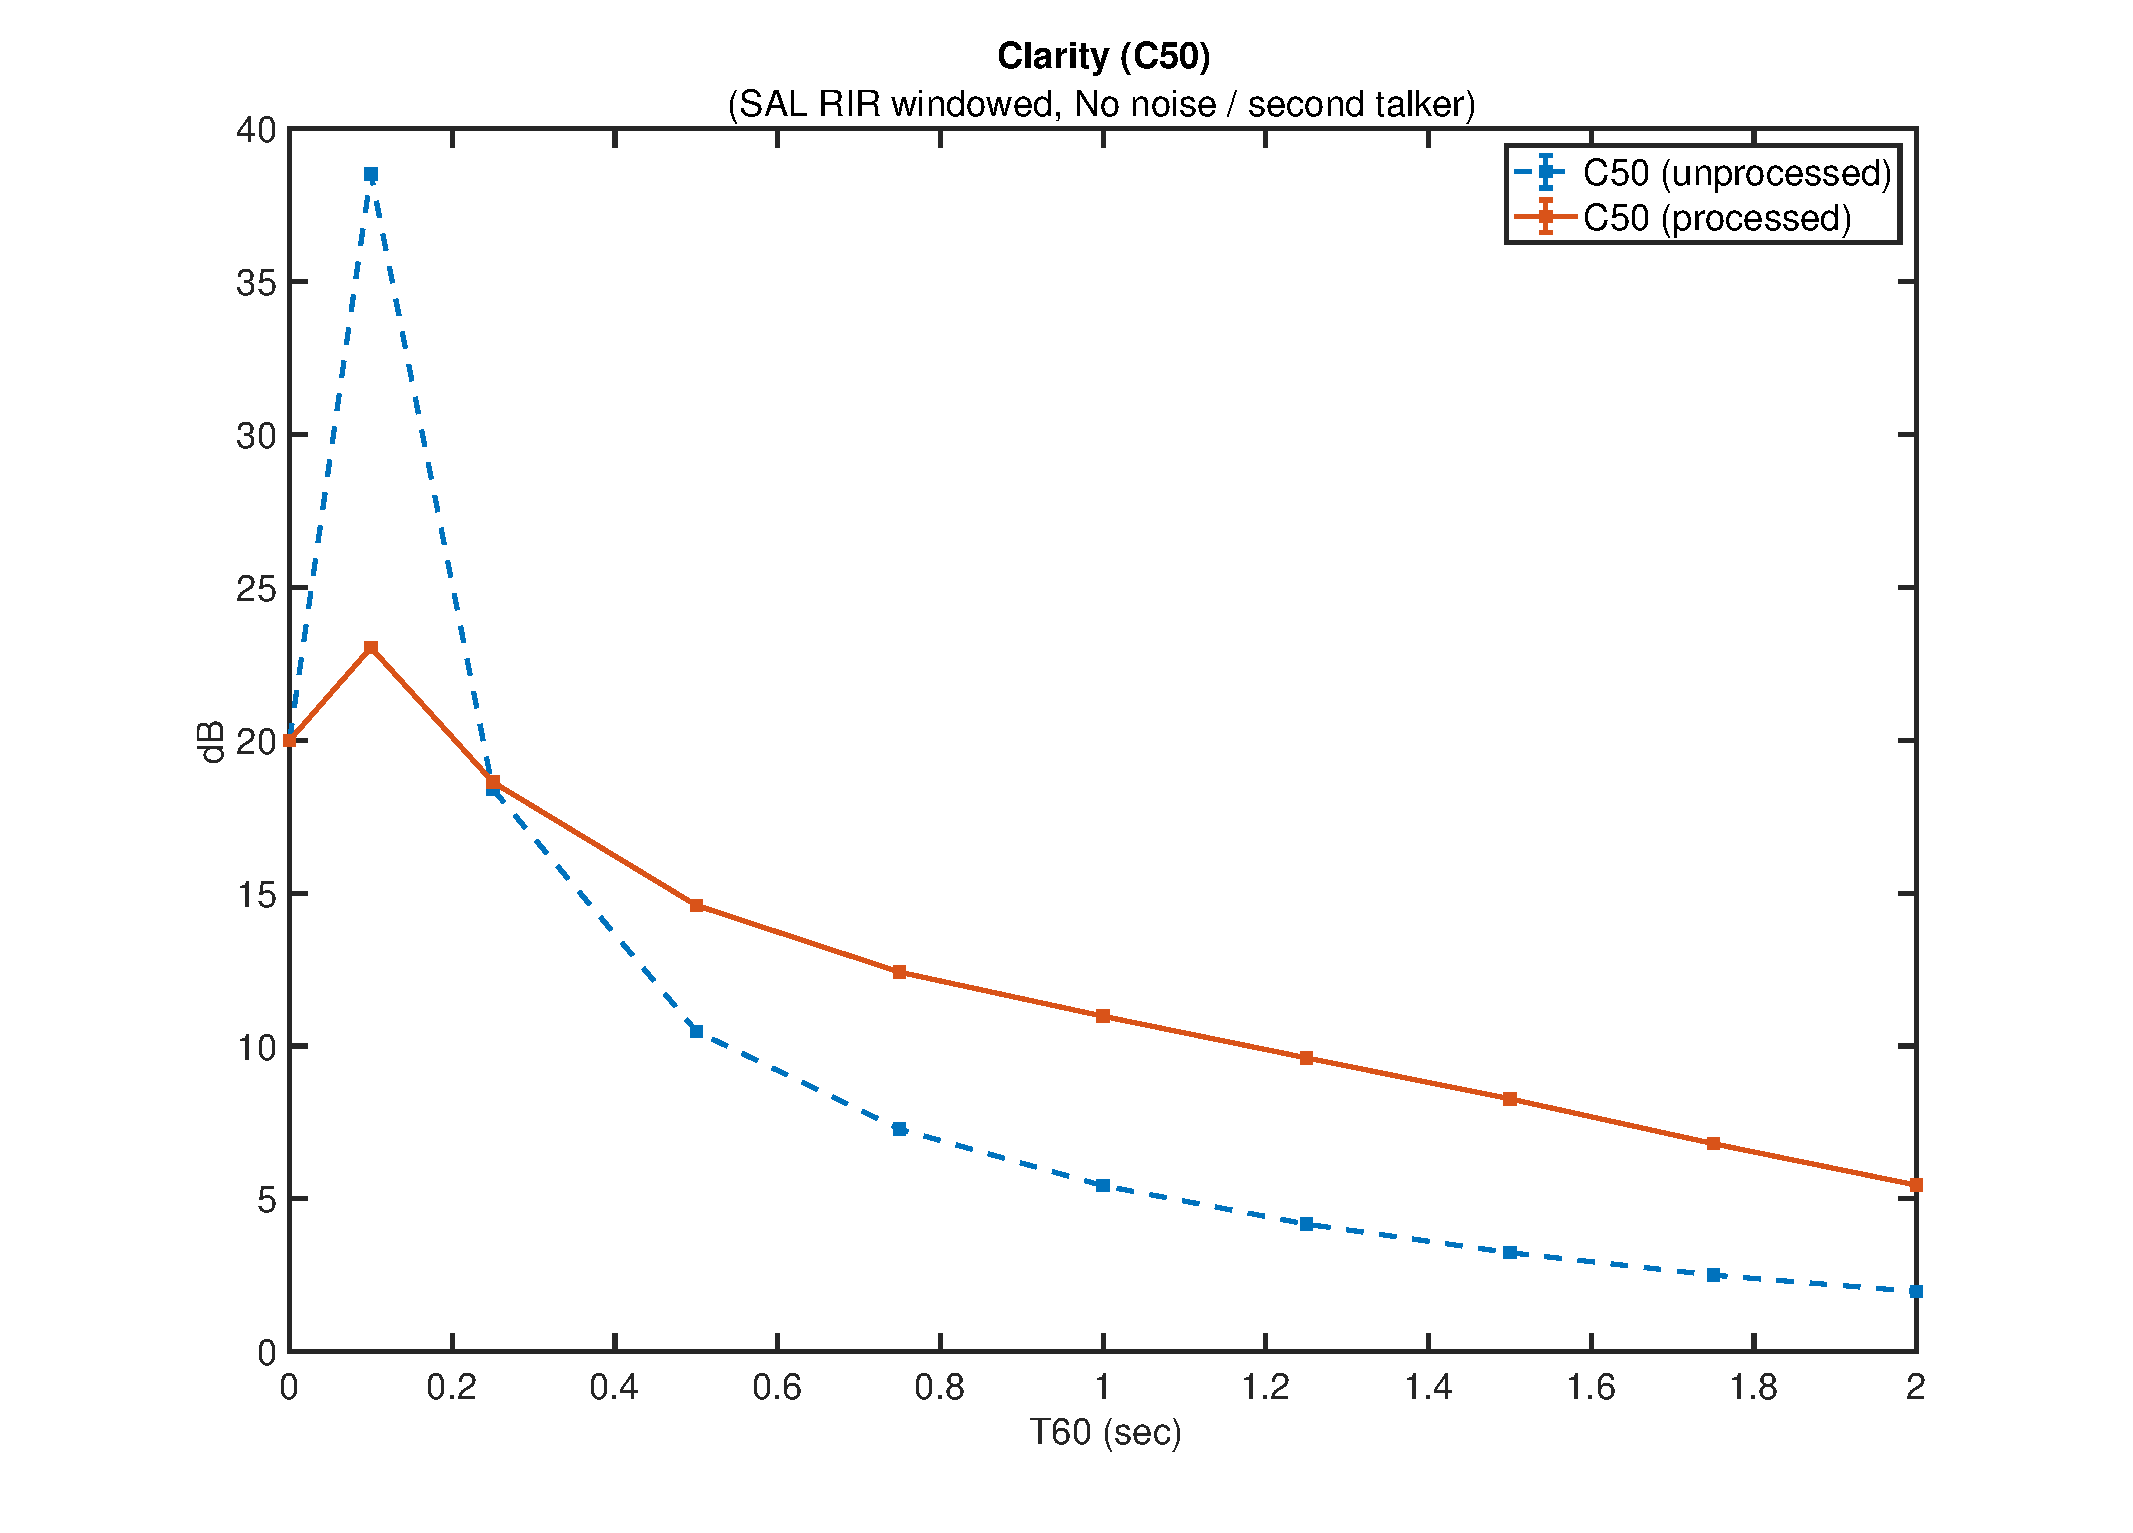
\includegraphics[width=\textwidth]{DAP_EVAL_1000T60max_noReg_C50_v_T60}
	\end{subfigure}
	\begin{subfigure}[b]{0.92\textwidth}
		\centering
		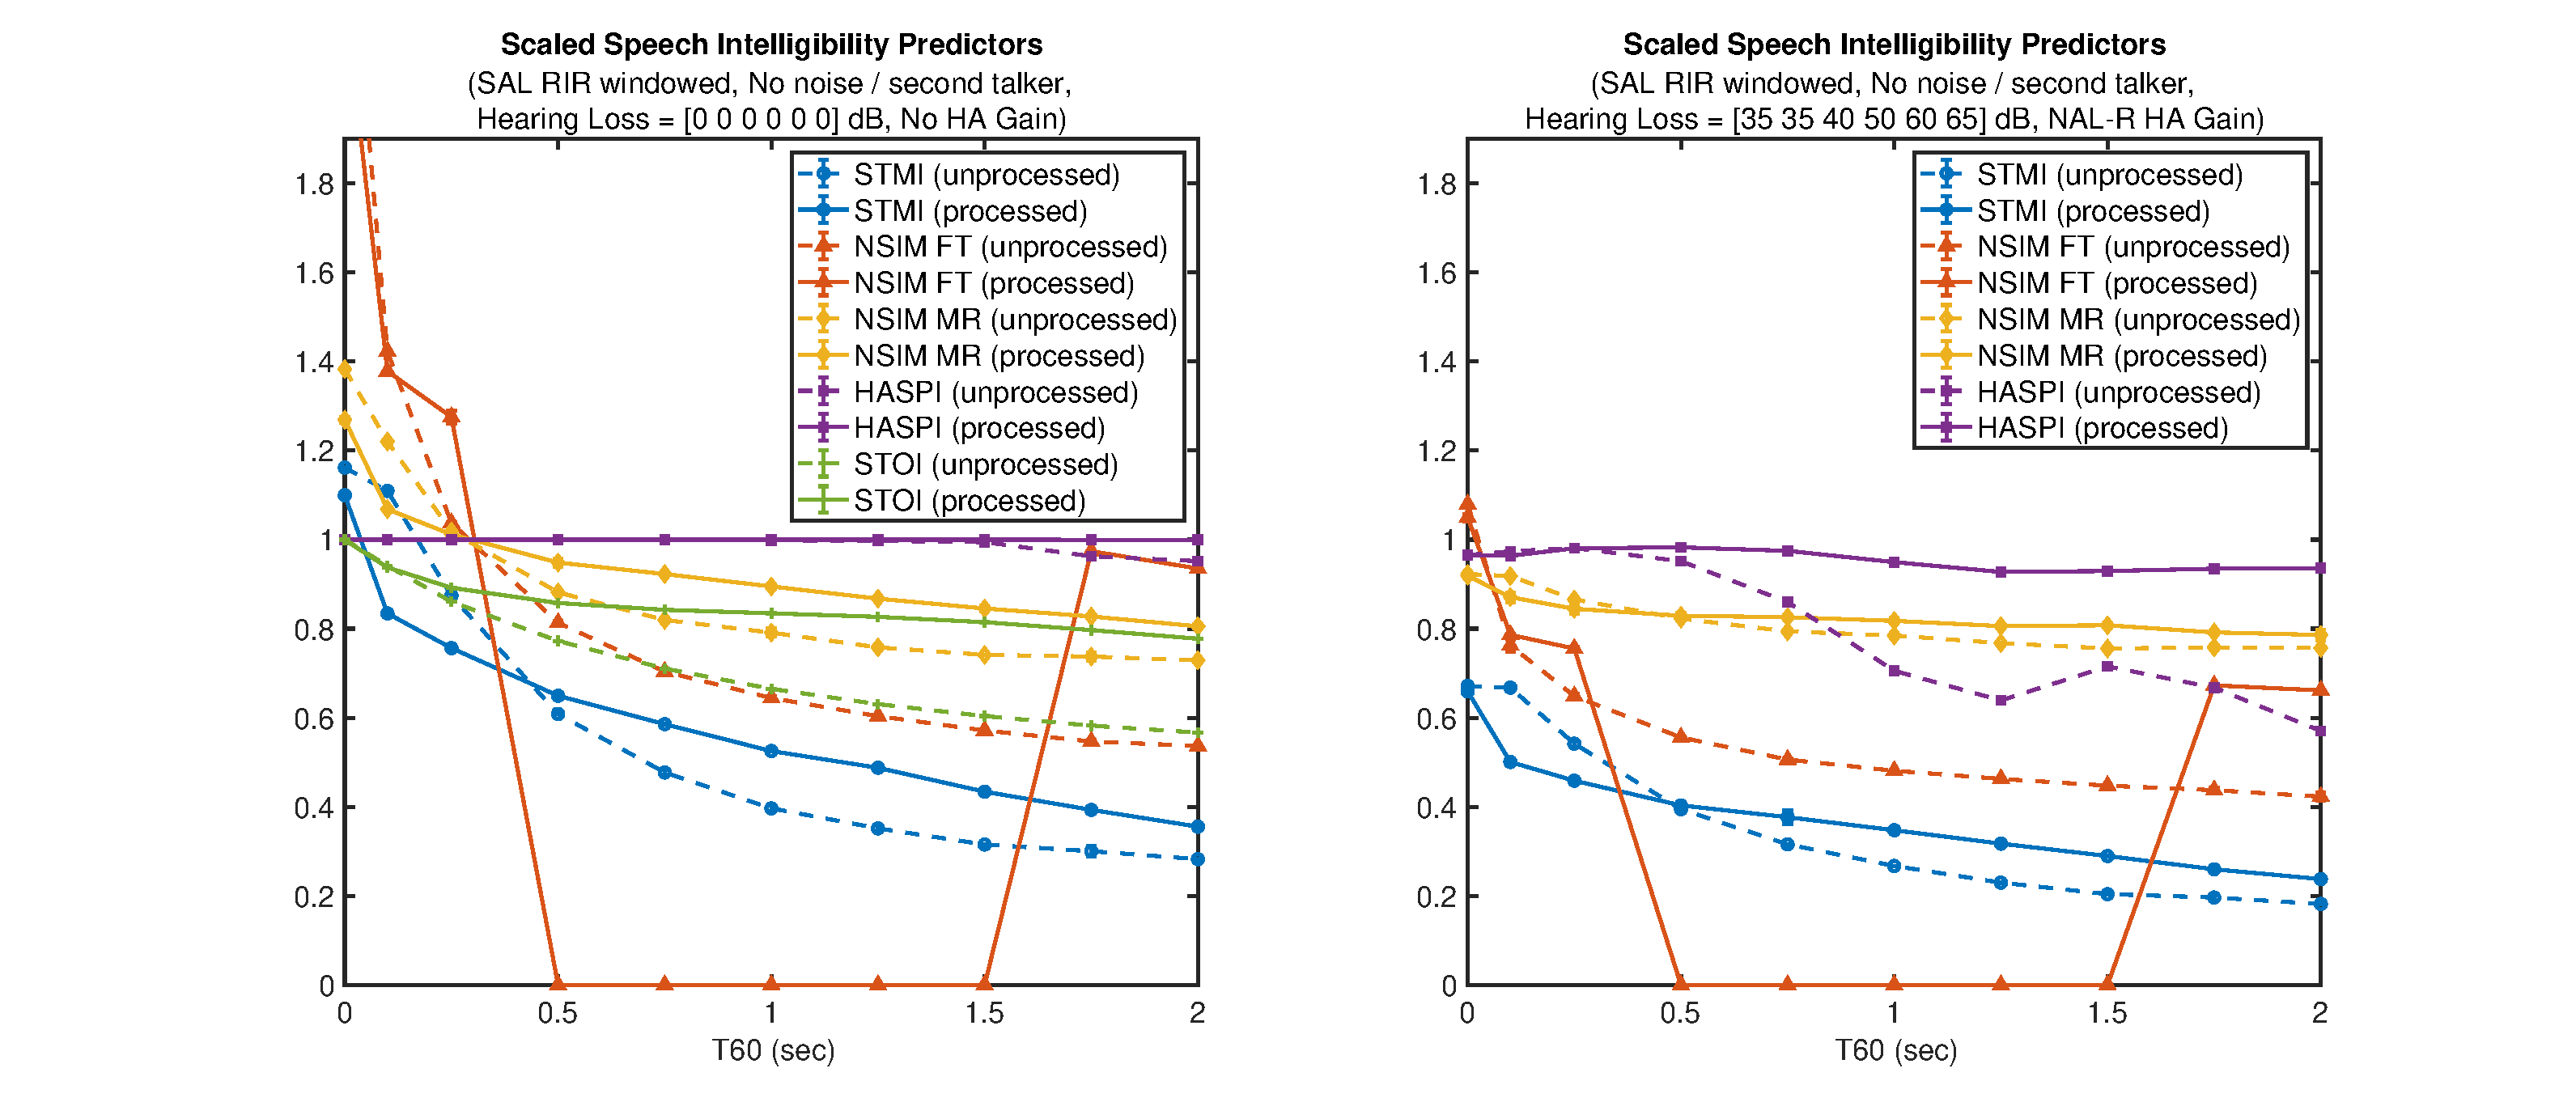
\includegraphics[width=\textwidth]{DAP_EVAL_1000T60max_noReg_SI_v_T60}
	\end{subfigure}
	\begin{subfigure}[b]{0.92\textwidth}
		\centering
		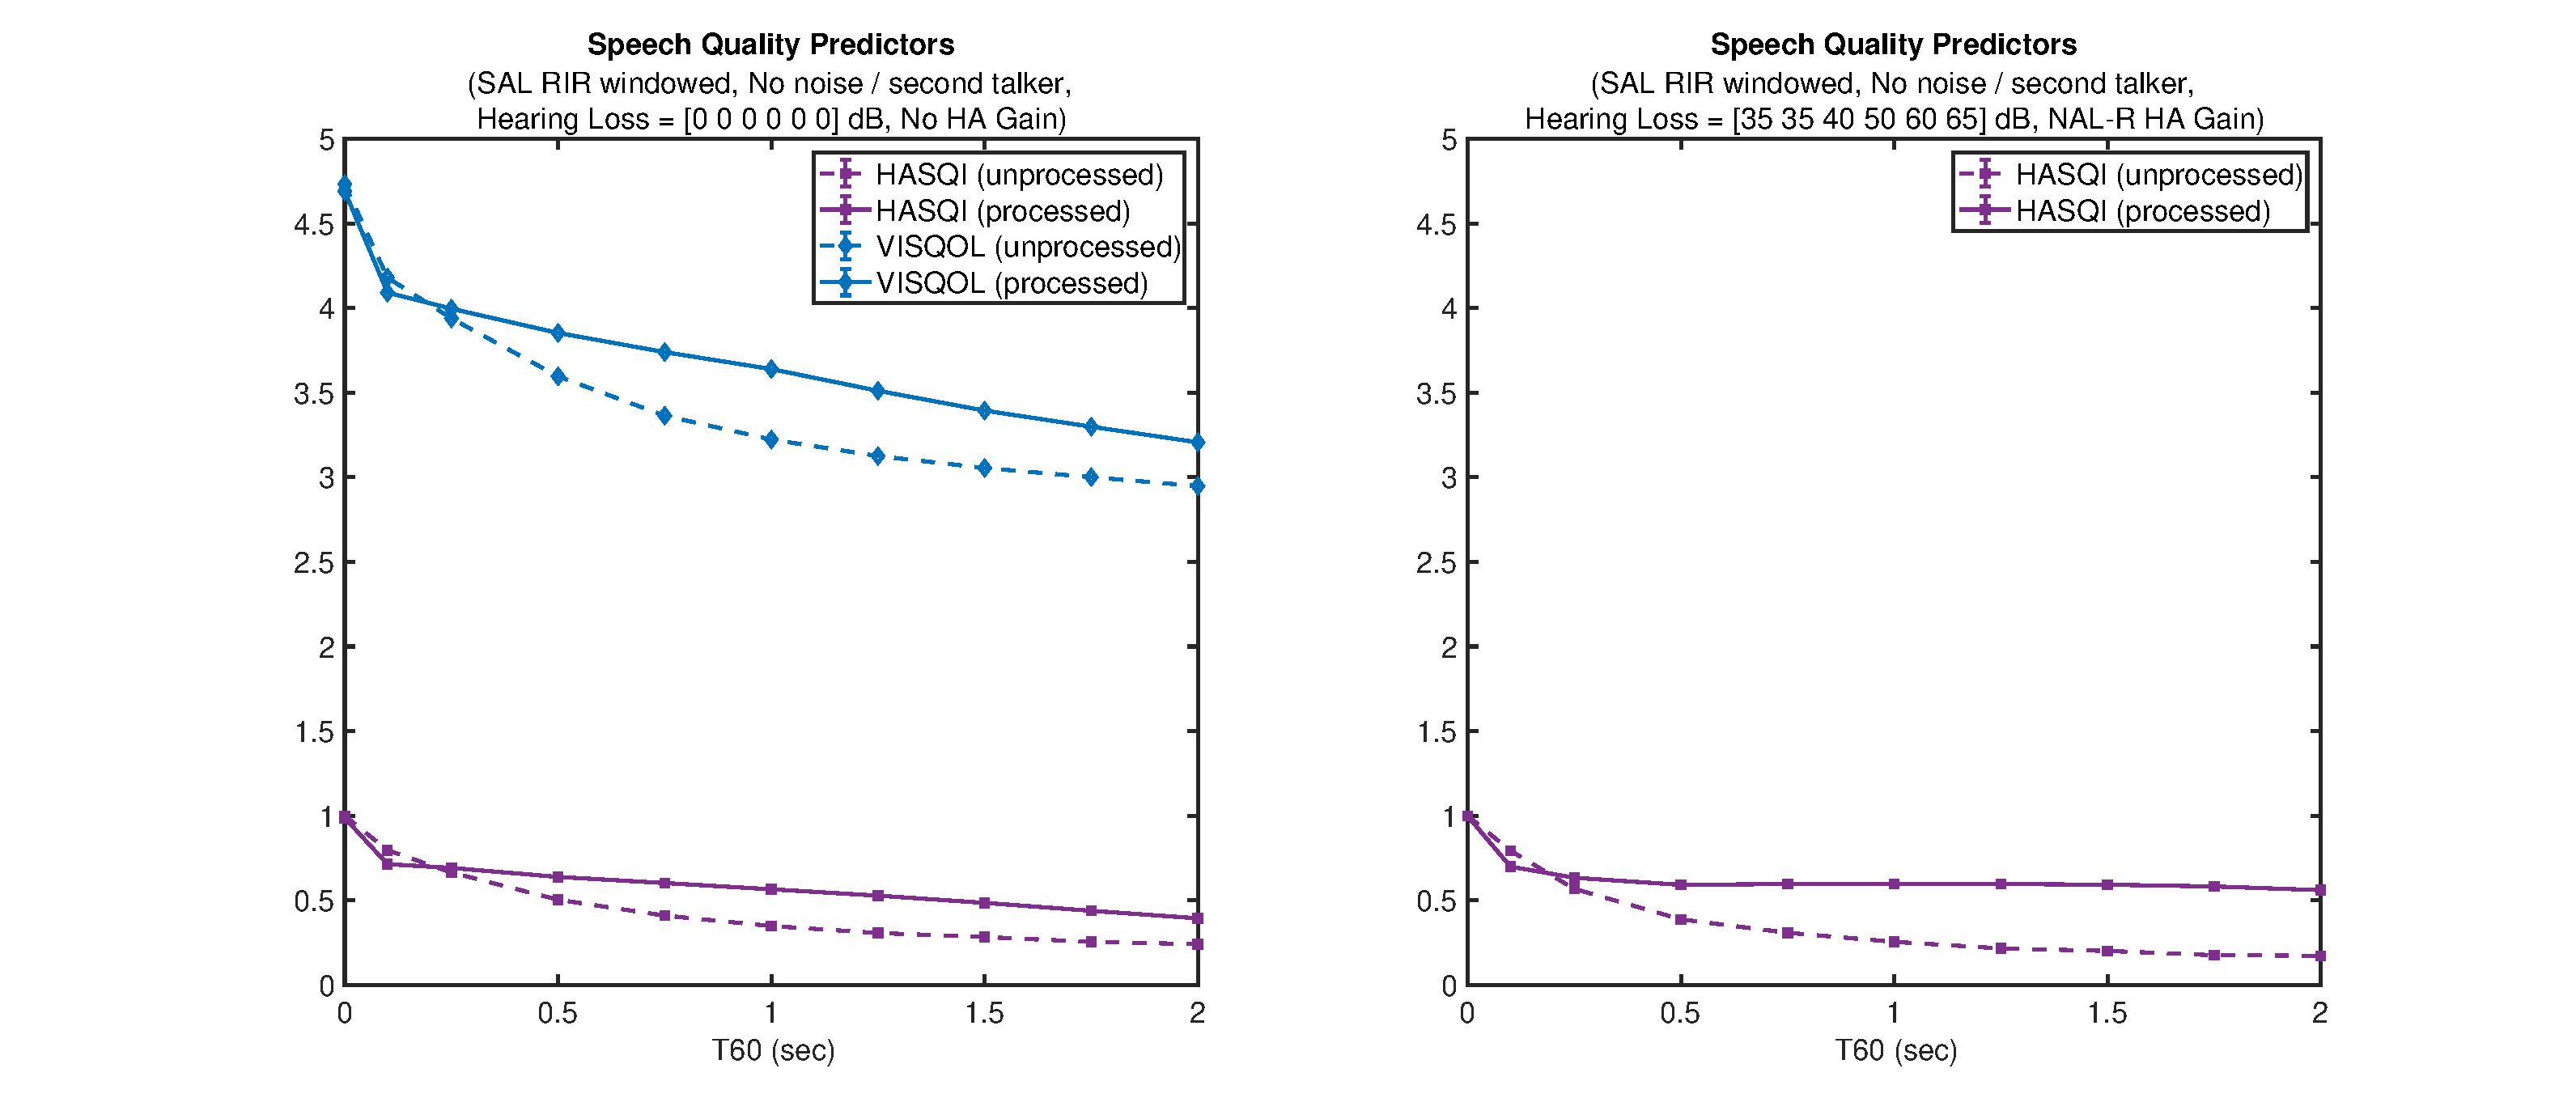
\includegraphics[width=\textwidth]{DAP_EVAL_1000T60max_noReg_SQ_v_T60}
	\end{subfigure}
	\caption[DAP evaluation with $p_2=5333$]{Evaluation of delay-and-predict dereverberation performance as a function of T60. Prediction orders were $p_2 = 5333$ and $p_1=20000$ (i.e., set according to $\mathrm{T60}_{\mathrm{max}} = \qty{1}{\sec}$ for$M=4$ and $f_s=\qty{16}{\kilo\hertz})$. RIRs were generated by applying a variable decay-rate exponential window to a measured RIR (The SAL room from the MYRiAD database, $\mathrm{T60} = \qty{2.2}{\second}$) to control T60. No Noise or Interfering talker were included.}
	\label{fig:DAP_EVAL_1000T60max_noReg}
\end{figure}


Firstly, it was noted that C50 results showed an improvement over most T60s, peaking at a C50 gain of approximately \qty{6}{\decibel} at a T60 of \qty{1}{\sec}. However, since DAP does not differentiate between cancellation of early reflections and late reflections, the algorithm was found to have a negative impact on C50 for T60s below \qty{250}{\milli\sec} where more early reflection energy was reduced than late reflection energy. Similarly, the algorithm was found to provide a boost in predicted SQ for all T60s above \qty{250}{\milli\sec}, reflecting impact of reduced reverberation on quality and the absense of any other algorithmic distortions that would have a negative impact on quality.

Generally all SI predictors showed that DAP provided a boost in perceptual performance. In the hearing impaired case, HASPI was found to increase from approximately 0.6 to 0.95 at $\mathrm{T60} = \qty{2}{\sec}$, suggesting that the algorithm almost completely restored SI. The improvements in MR-NSIM and STMI were more subtle, reflecting the fact that the ENV acoustic cues were not completely restored, and that the residual reverberation likely would still impact LE if not SI. Recall that the NSIM and STMI values were normalized such that a value of 1.0 is achieved for the clean speech convolved with only direct sound and early reflections without hearing loss. Therefore the NSIM/STMI values can be interpreted roughly a ratio of the corresponding acoustic cues that are represented with sufficient fidelity. 

The FT-NSIM results generally showed an improvement, suggesting that TFS cues were at at least partially restored. However, FT-NSIM was found to decrease at certain T60s. This was explained by the fact that the SSIM neurogram image comparison that underlies the NSIM is sensitive to subtle pixel shifts in the time axis, making the FT-NSIM very sensitive to phase distortions. The MC-LP prediction error equalizer in the DAP algorithm has zero algorithmic delay overall (as do all LP prediction error filters) because of the branch of the filter that passes one of the signals through unprocessed (i.e., the first FIR coefficient is $b_0=1$). However, the prediction error filter is also non-linear phase and therefore imposes phase distortions. These phase distortions are minimum due to the minimum-phase constraint imposed by the autocorrelation method of LP, but are non-negligible. It is at this point unclear whether these phase distortions have a significant impact on SI/LE. Therefore when interpreting the FT-NSIM results, it is reasonable to say that an increase in value implies restoration of TFS cues, but a decrease in value has an unclear meaning. There is therefore a need for more research into the perceptual impact of phase distortions to determine the perceptual validity of the NSIM as a predictor of SI/LE. This was left for future work.

For a closer look at the behaviour of the algorithm in this evaluation, the EIR and EDC performance for a T60 of \qty{1}{\sec} are shown in Figure \ref{fig:DAP_EVAL_1000T60max_noReg_EDCExample}. 

\begin{figure}[H]
	\centering
	\begin{subfigure}[b]{0.42\textwidth}
		\centering
		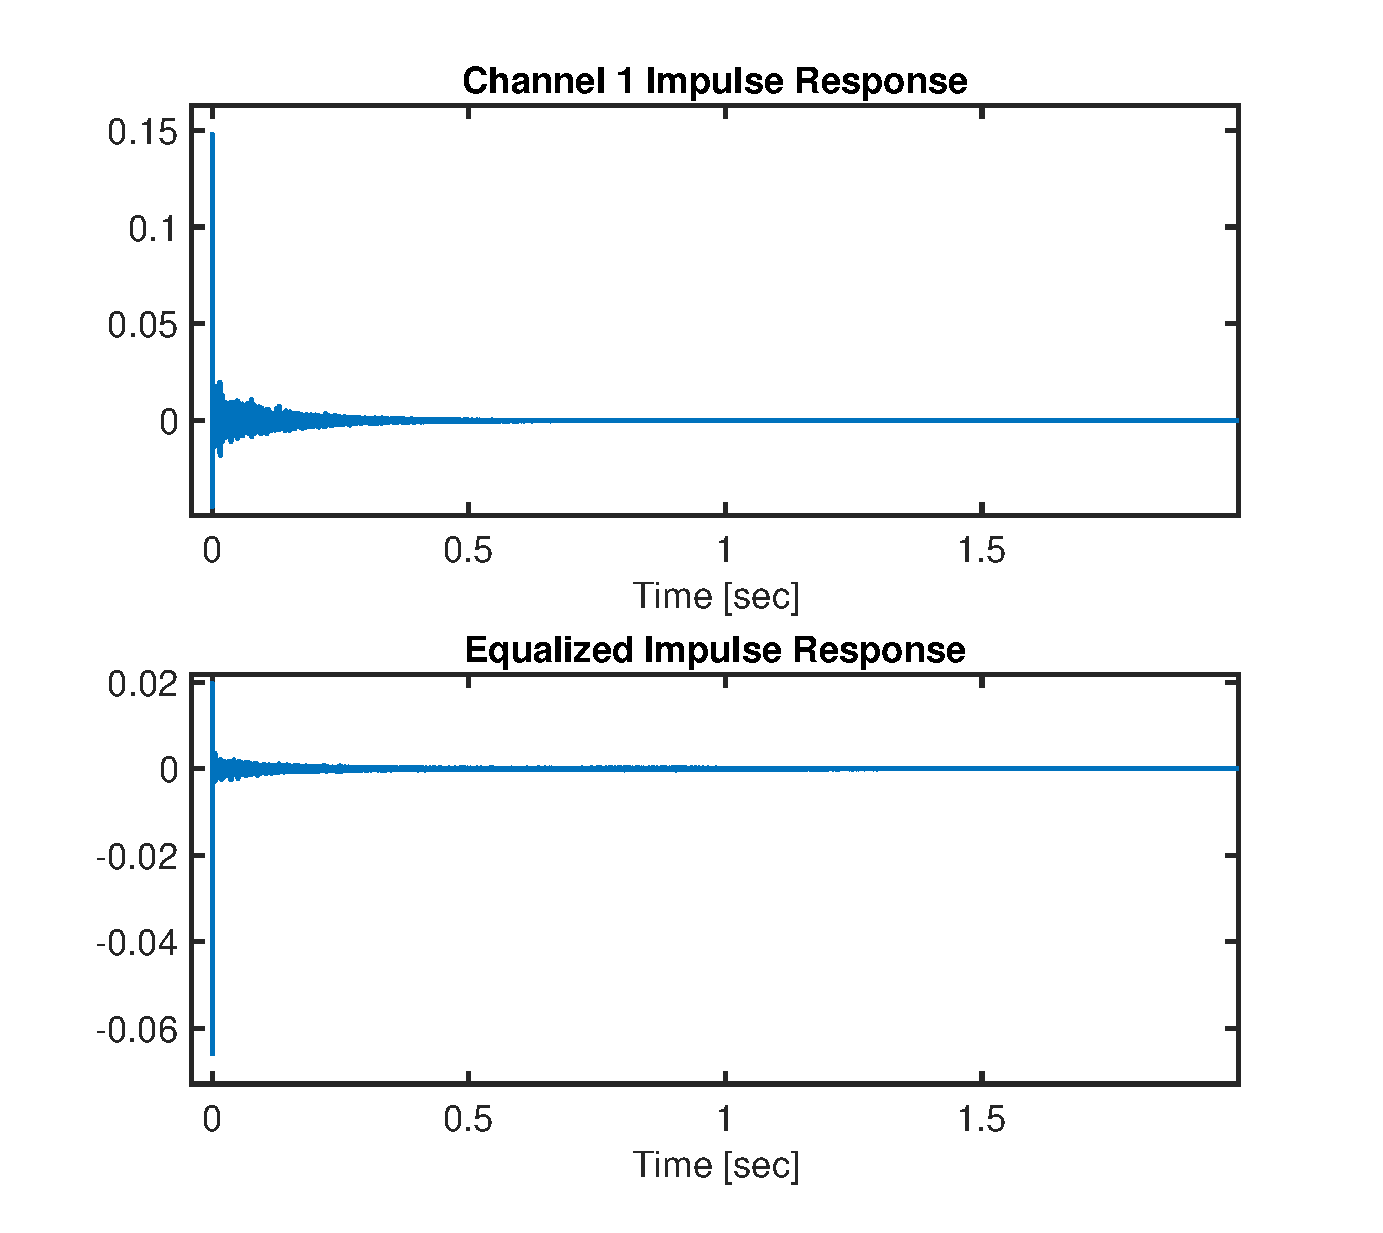
\includegraphics[width=\textwidth]{DAP_EVAL_1000T60max_noReg_EIRExample_1sec}
	\end{subfigure}
	\begin{subfigure}[b]{0.45\textwidth}
		\centering
		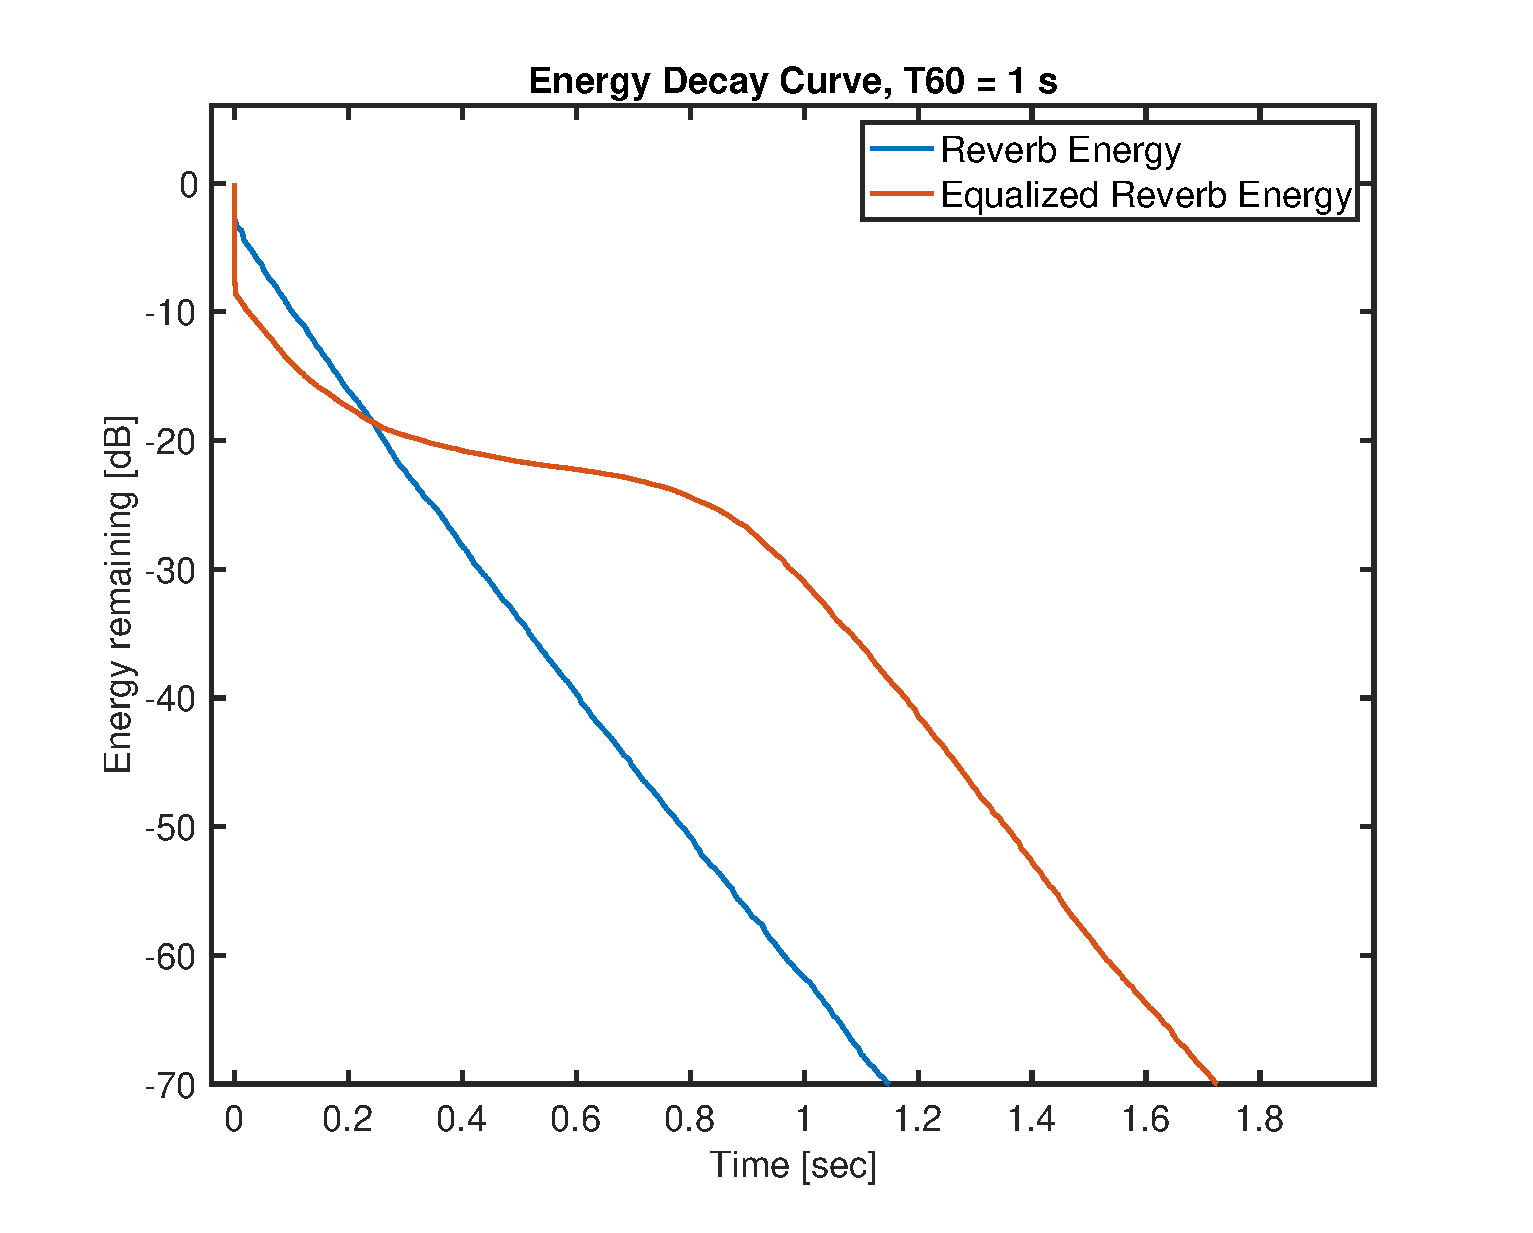
\includegraphics[width=\textwidth]{DAP_EVAL_1000T60max_noReg_EDCExample_1sec}
	\end{subfigure}
		\caption[EDC example from DAP Evaluation with $p_2=5333$]]{EDC and EIR performance from a single iteration of the results shown in Figure \ref{fig:DAP_EVAL_1000T60max_noReg} for a T60 of \qty{1}{\sec}}
	\label{fig:DAP_EVAL_1000T60max_noReg_EDCExample}
\end{figure}

Although the prediction orders were selected as per the discussion in Section \ref{section:params_conclusion} to optimally cancel a T60 of \qty{1}{\sec} (i.e., prediction orders $p_2=5333$ and $p_1=20000$), the EDC was only found to show reduction in reverberation up to the \qty{250}{\milli\sec}. This is because the limited amount of signal data used in this evaluation was insufficient to reduce the amount of autocorrelation variance that occurs at the lags dictated by the prediction orders. Therefore the experiment was repeated with prediction orders set to optimally cancel a T60 of \qty{500}{\milli\sec} (i.e., $p_2=2667$ and $p_1=10000$) to reduce computations. The results are shown in Figure \ref{fig:DAP_EVAL_500T60max_noReg}.

%Limited cancellation acheived for T60 > 500ms (Due to estimation variance). Reduced max T60 to 500 ms. Tuned based on a T60 of 500 ms in chapter 3, equation based on T60 doesnt really apply as T60s get very long because estimation variance becomes increasingly a limiting factor.

\begin{figure}[H]
	\centering
	\begin{subfigure}[b]{0.47\textwidth}
		\centering
		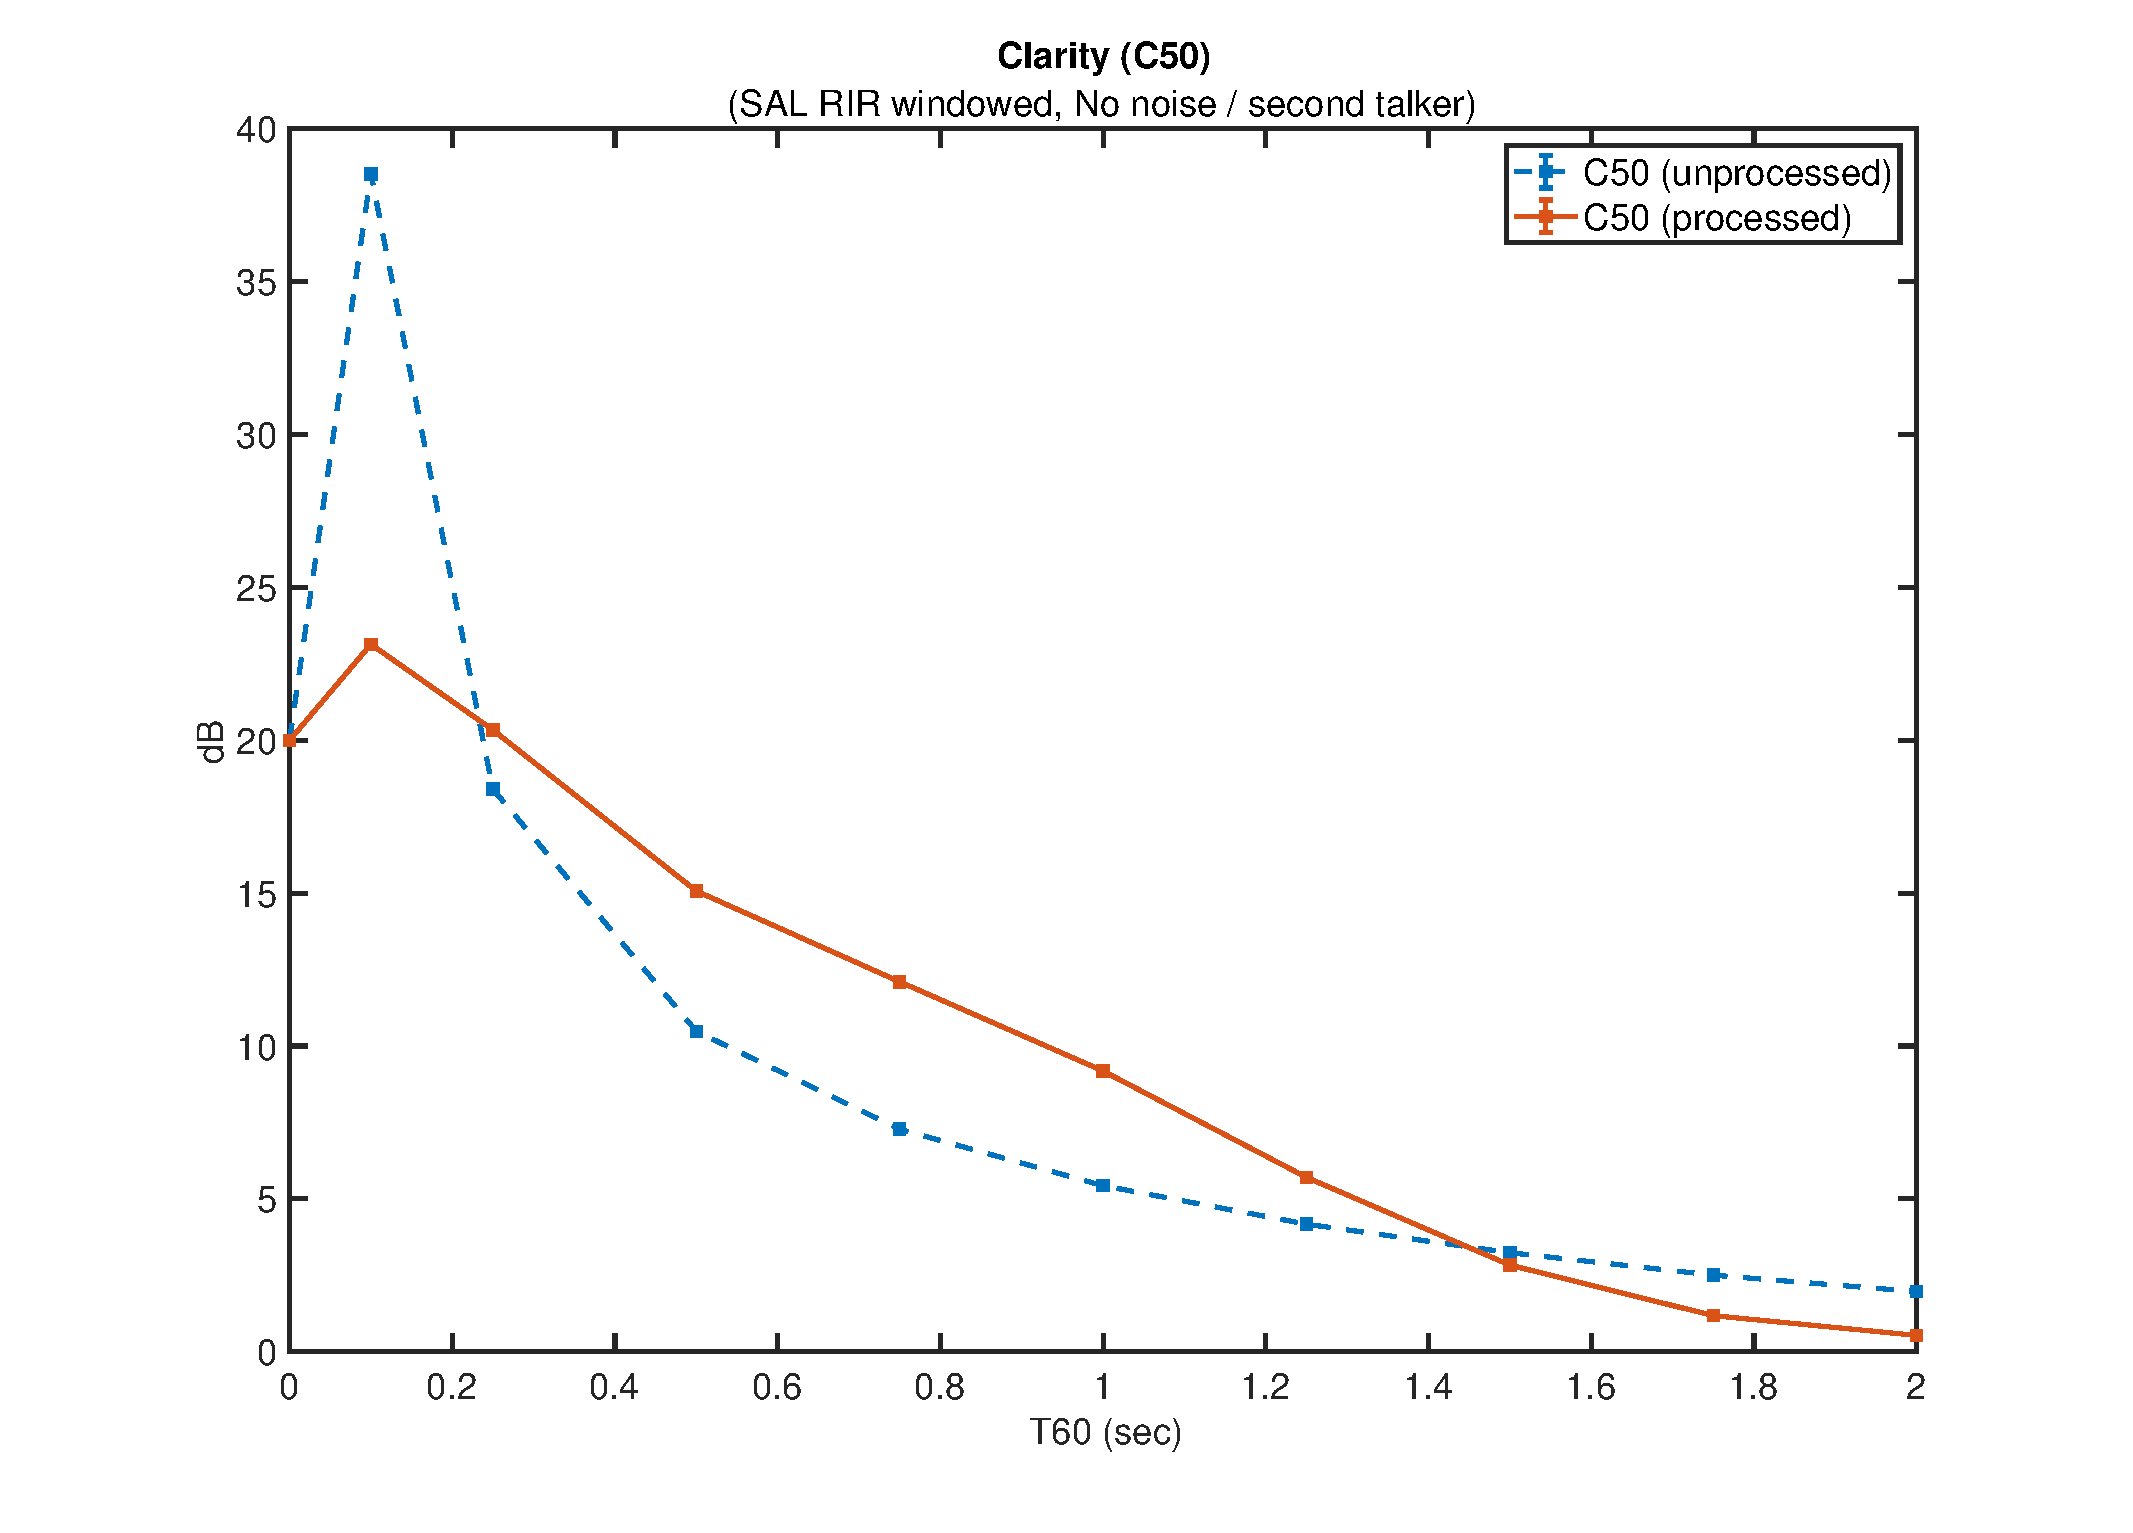
\includegraphics[width=\textwidth]{DAP_EVAL_500T60max_noReg_C50_v_T60}
	\end{subfigure}
	\begin{subfigure}[b]{0.92\textwidth}
		\centering
		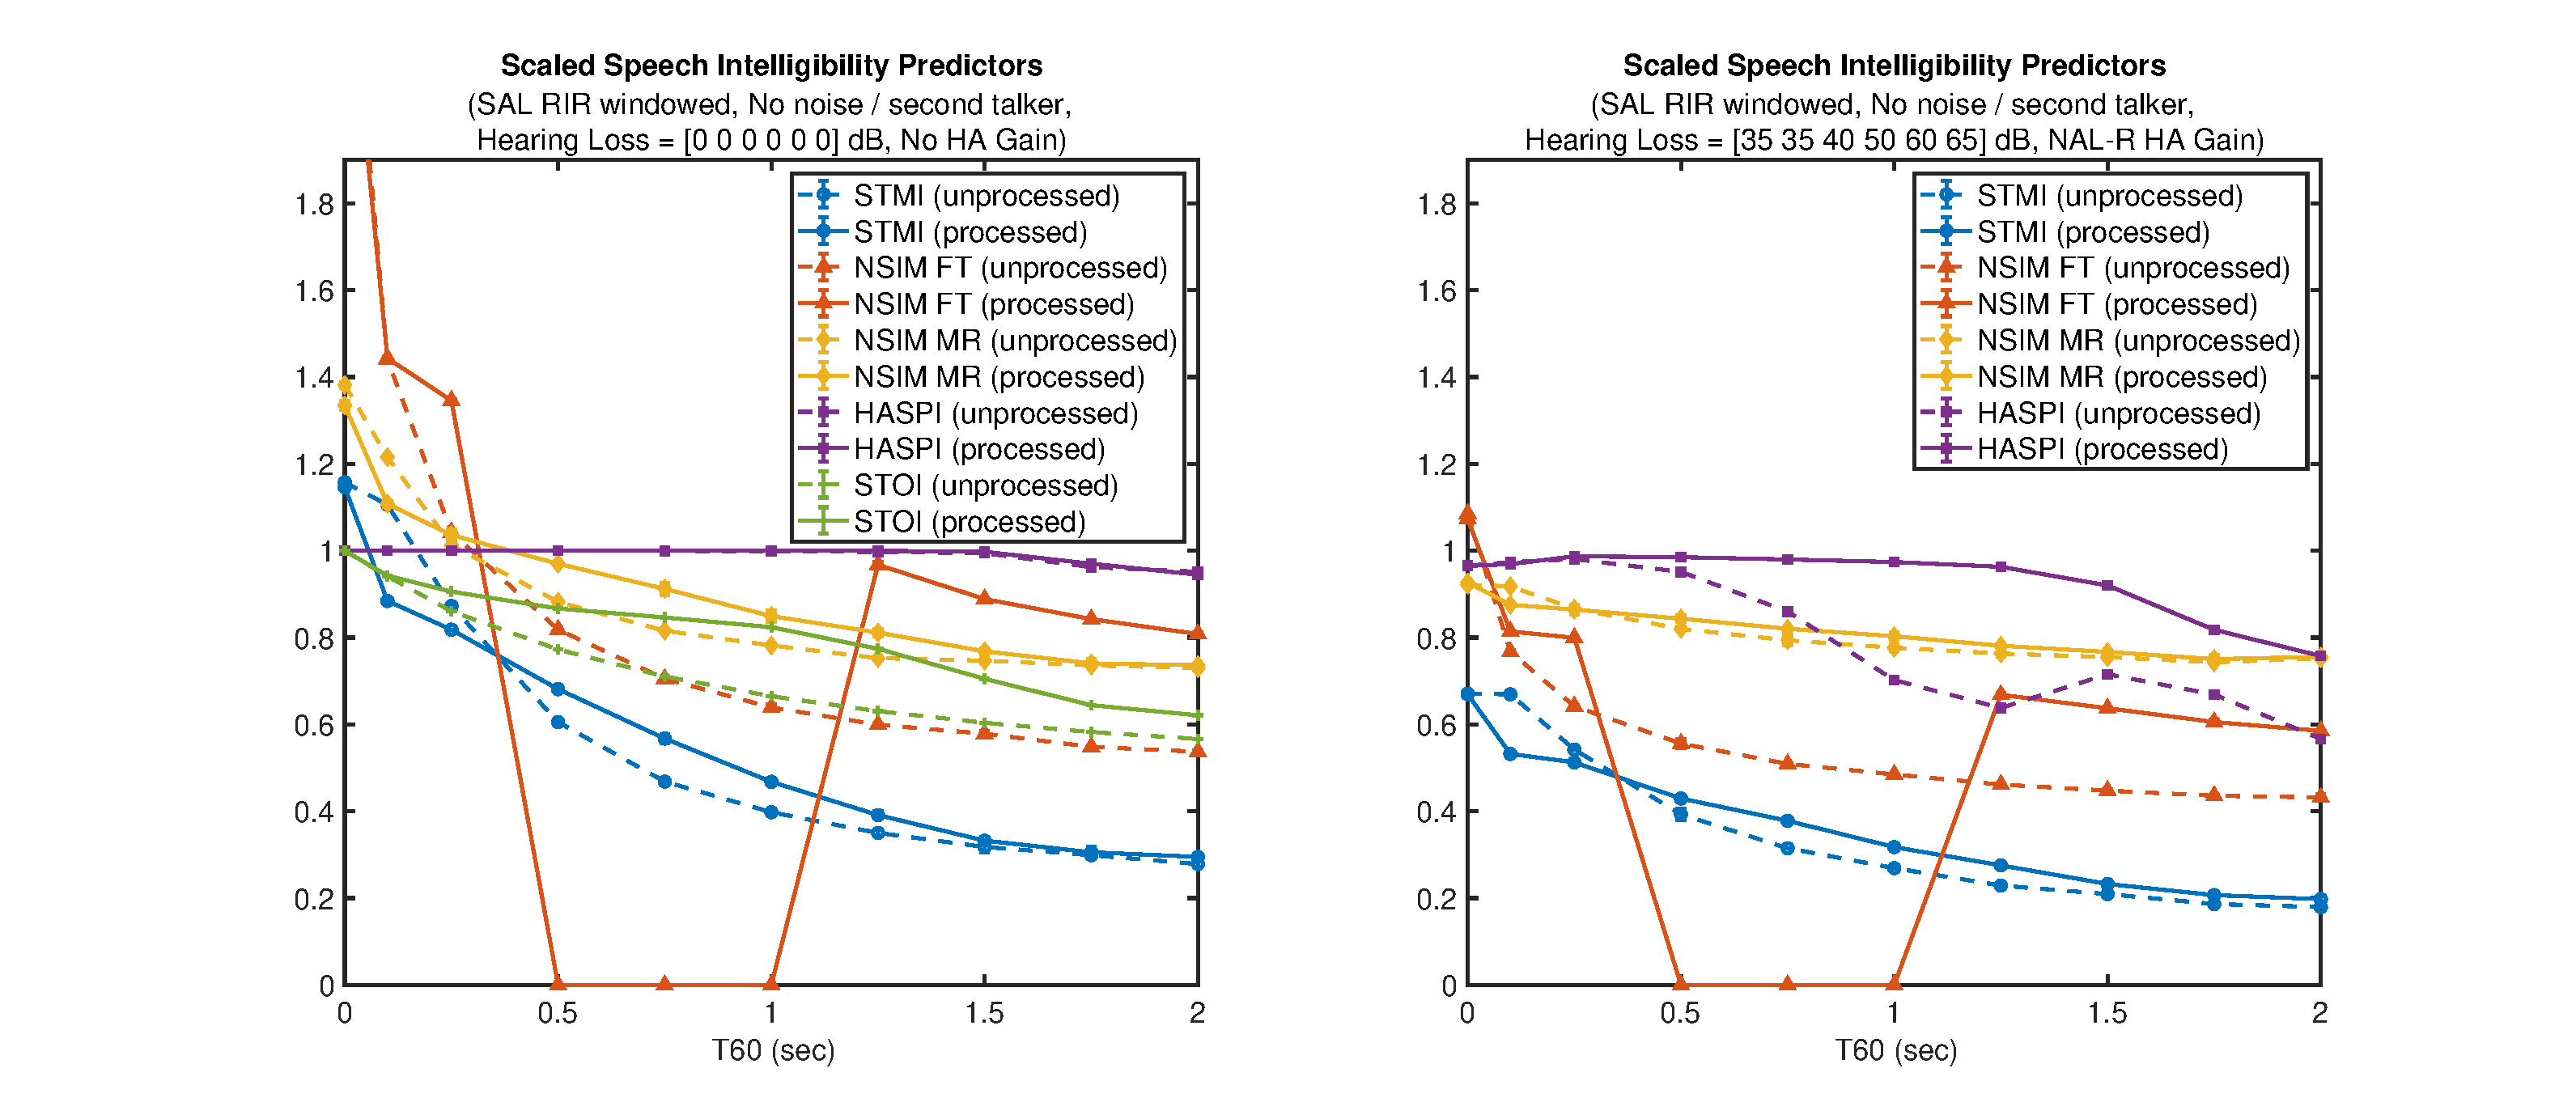
\includegraphics[width=\textwidth]{DAP_EVAL_500T60max_noReg_SI_v_T60}
	\end{subfigure}
	%\begin{subfigure}[b]{0.92\textwidth}
	%	\centering
	%	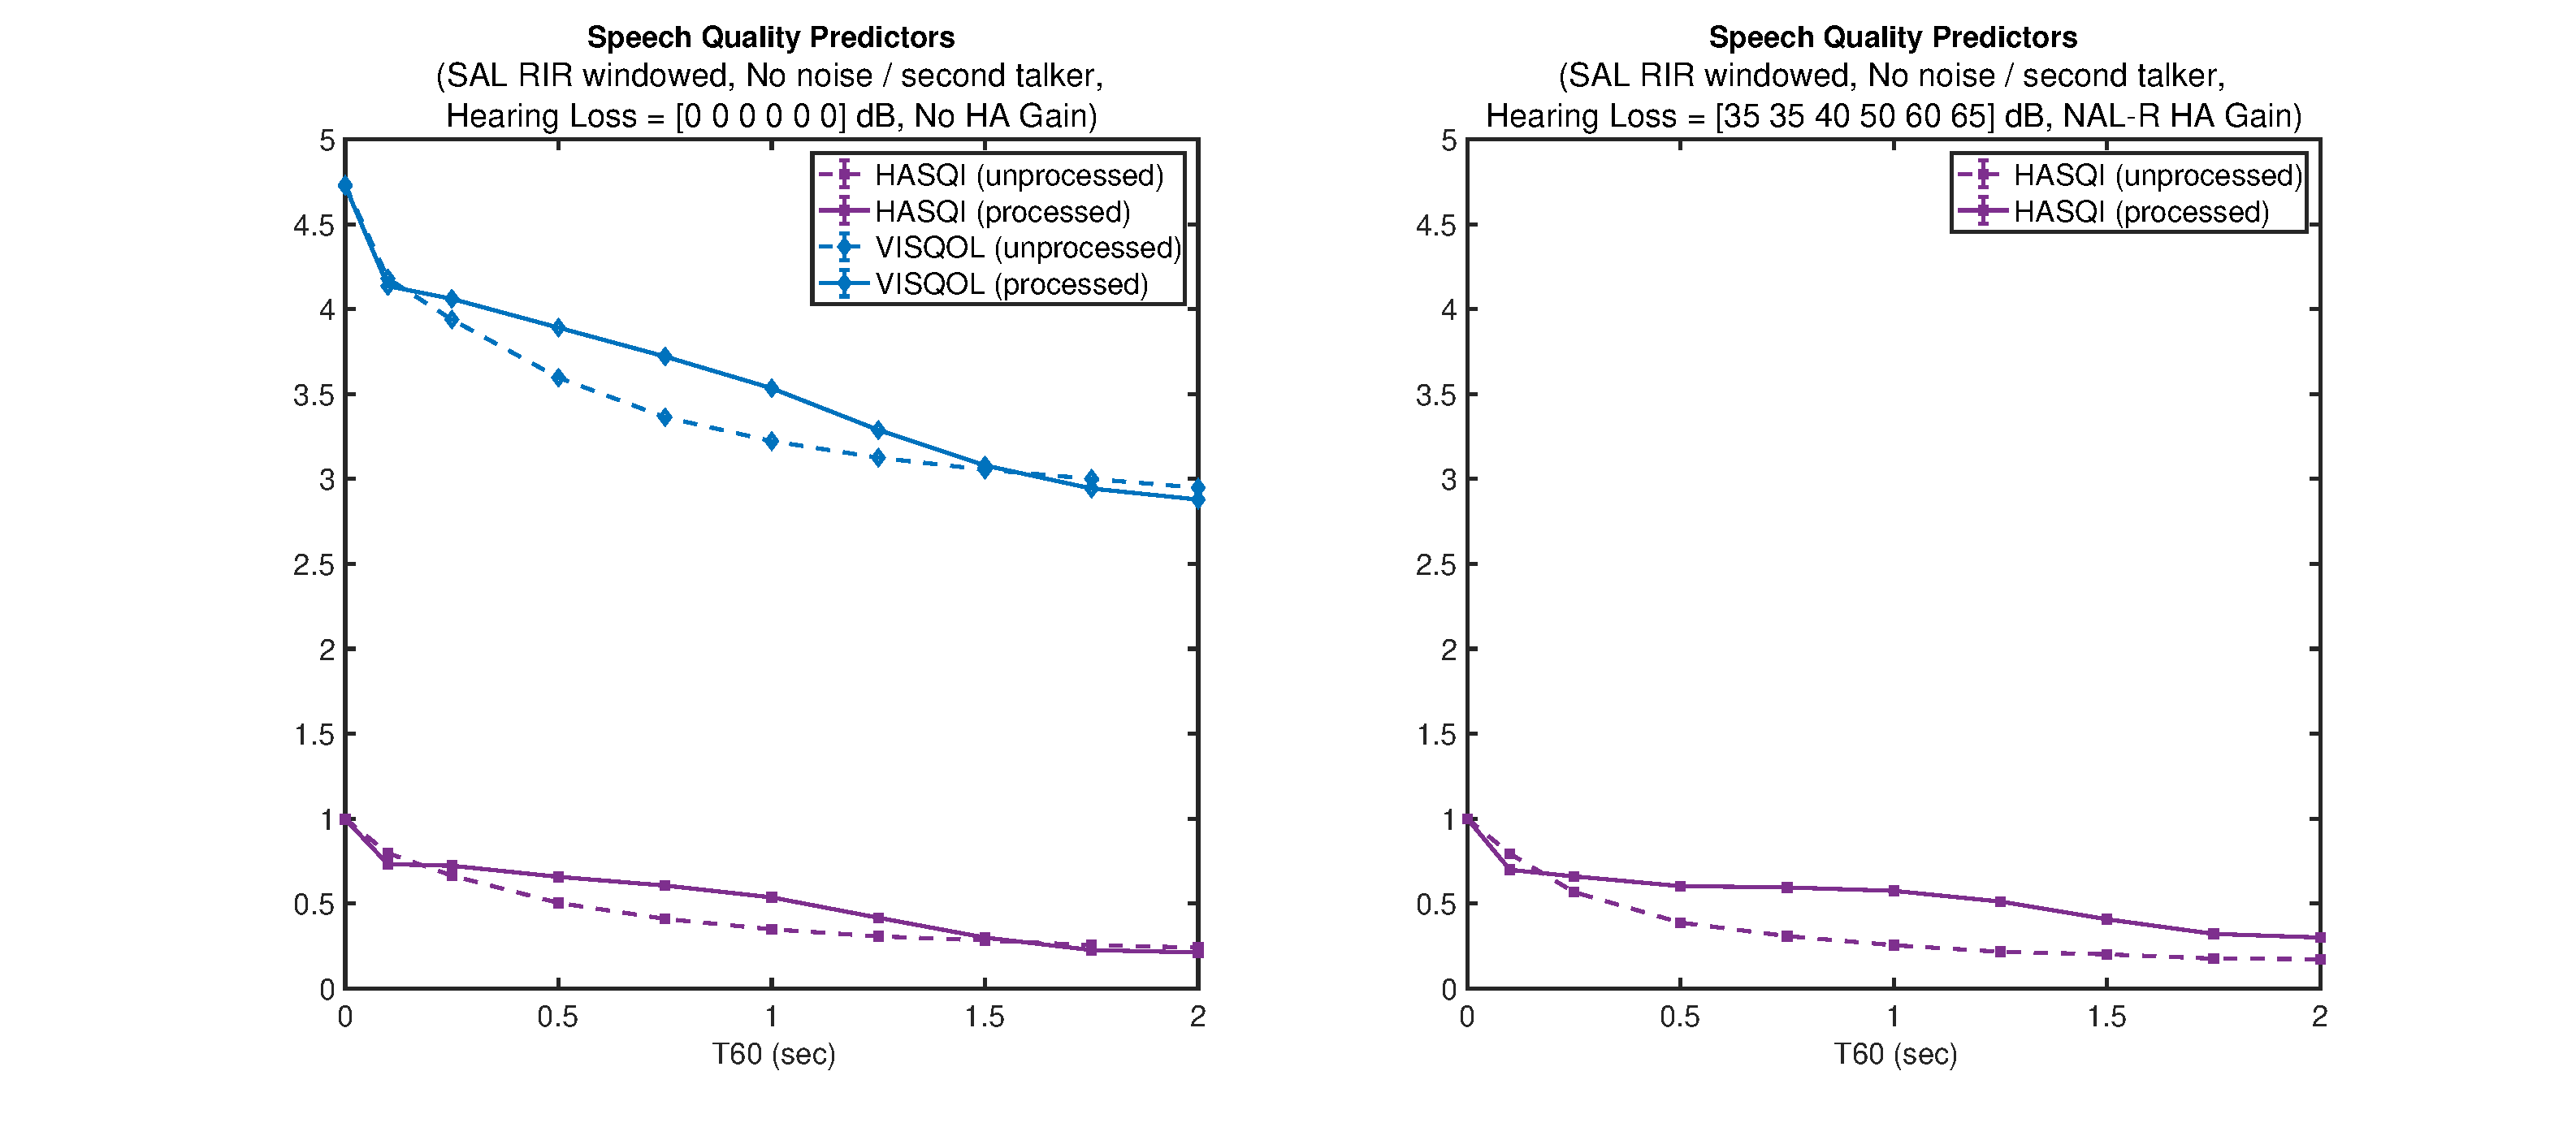
\includegraphics[width=\textwidth]{DAP_EVAL_500T60max_noReg_SQ_v_T60}
	%\end{subfigure}
	\caption[DAP Evaluation with $p_2=2667$]]{Evaluation of delay-and-predict dereverberation performance as a function of T60. Prediction orders were $p_2 = 2667$ and $p_1=10000$ (i.e., set according to $\mathrm{T60}_{\mathrm{max}} = \qty{500}{\milli\sec}$ for $M=4$ and $f_s=\qty{16}{\kilo\hertz})$. RIRs were generated by applying a variable decay-rate exponential window to a measured RIR (The SAL room from the MYRiAD database, $\mathrm{T60} = \qty{2.2}{\second}$) to control T60. No Noise or Interfering talker were included.}
	\label{fig:DAP_EVAL_500T60max_noReg}
\end{figure}

In this experiment, similar perceptualy performance to the previous experiment was observed accross all predictors of SI and SQ for lower T60s, but for very high T60s performance dropped off and the algorithm was observed to actually make things worse. As discussed in Section \ref{section:params_p2_MC_LP} , the equalizer generated by MC-LP does a good job of cancelling the early part of the RIR, but towards the end of the time spanned by the equalizer, reverberation energy can actually increase due higher estimation variance at longer autocorrelation lags (as shown in Figure \ref{subfig:EDC_500T60_500T60max_NoReg} below). This effect was initially accepted as an inevitable side effect of MC-LP-based reverberation cancellation, and it was assumed that the benefits in the early part of the RIR would outweigh the negative side effects in the later/weaker part of the RIR.  However, it is clear from this evaluation that for very long reverberation times, the increase in late reverberation becomes significant and the perceptual impact is non-negligible. This makes sense because for longer reverberation times, the energy of the reverberation in the vicinity of high autocorrelation variance is higher, and therefore the impact of the variance is more pronounced. Moreover, while ENV acoustic cues are have a larger dynamic range / energy and are therefore not significantly impacted by low-level reverberation, TFS acoustic cues are more heavily distorted by low-level reverberation. As discussed in Section \ref{section:encoding_acoustic_cues}, in mild reverberation the fidelity of TFS cues generally only impacts LE, but in more severe reverberation, TFS fidelity can impact SI.

% XXXX = \ref{subfig:EDC_500T60_500T60max_NoReg} 

Since the increase in autocorrelation variance occurs at long lags where the reverberant energy is generally lower, It was hypothesized that adding a small amount of autocorrelation regularization could reduce this side effect without significantly reducing performance in the earlier/higher energy part of the RIR. This was done by adding a small offset ($\psi = 2.5 \times 10^{-5}$) to the diagonal entires of the spatially averaged temporal autocorrelation matrix that is used in the source-whitening stage (i.e., $\boldsymbol{R}_{\mathrm{avg}}$ in Equation \ref{eq:dap_source_whitening_yule_walker}) and also to the multichannel spatio-temporal correlation matrix used in the MC-LP stage  (i.e., $\boldsymbol{R}_{\mathrm{mc}}$ in Equation \ref{eq:dap_mc_lp_yule_walker}). Regularization of autocorrelation matrices in LP Yule-Walker equations has the effect of improving numerical stability and making the resulting prediction error filters more white. The impact of this regularization on EIR/EDC performance is shown in Figure \ref{fig:params_regularization_500T60}.

\begin{figure}[H]
	\centering
	% Without Regularization
	\begin{subfigure}[b]{0.42\textwidth}
		\centering
		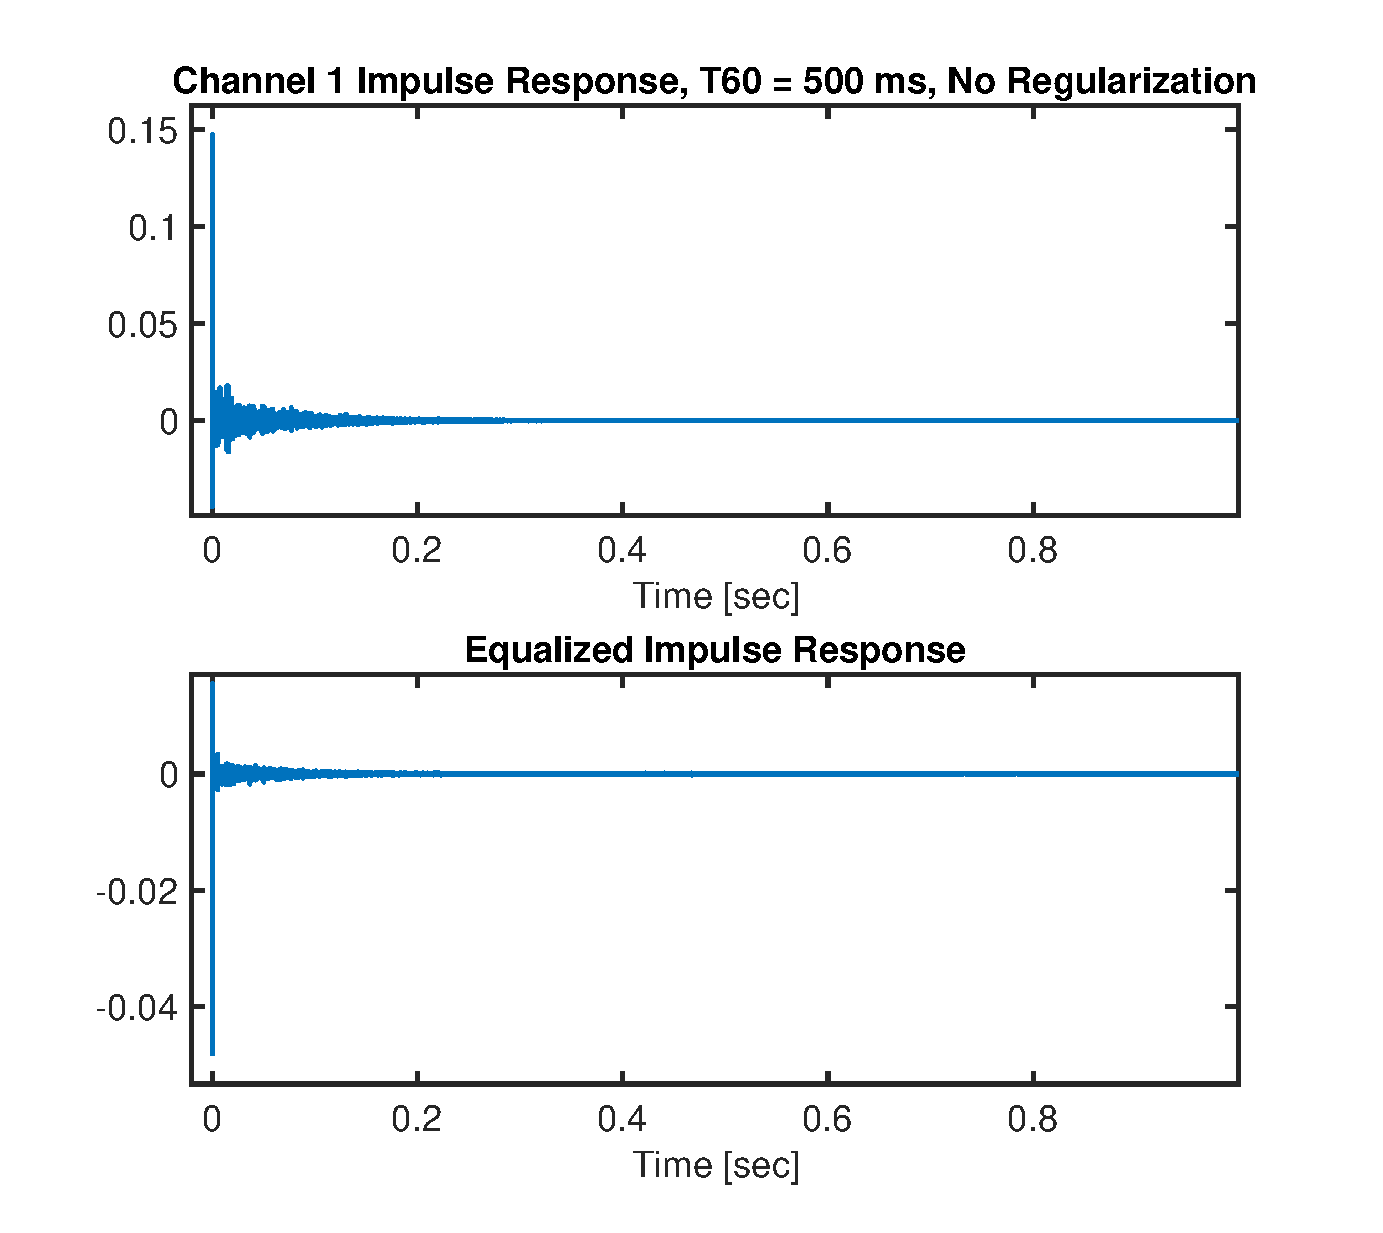
\includegraphics[width=\textwidth]{EIR_500T60_500T60max_NoReg}
		\subcaption{}
		\label{subfig:EIR_500T60_500T60max_NoReg}
	\end{subfigure}
	\begin{subfigure}[b]{0.45\textwidth}
		\centering
		\includegraphics[width=\textwidth]{EDC_500T60_500T60max_NoReg}
		\subcaption{}
		\label{subfig:EDC_500T60_500T60max_NoReg}
	\end{subfigure}
	
	% With Regularization
	\begin{subfigure}[b]{0.42\textwidth}
		\centering
		\includegraphics[width=\textwidth]{EIR_500T60_500T60max_wReg}
		\subcaption{}
		\label{subfig:EIR_500T60_500T60max_wReg}
	\end{subfigure}
	\begin{subfigure}[b]{0.45\textwidth}
		\centering
		\includegraphics[width=\textwidth]{EDC_500T60_500T60max_wReg}
		\subcaption{}
		\label{subfig:EDC_500T60_500T60max_wReg}
	\end{subfigure}
	\caption[EDC Impact of autocorrelation regularization]{Impact of autocorrelation matrix regularization on dereverberation performance.  Prediction orders were $p_2 = 2667$ and $p_1=10000$ (i.e., according to $\mathrm{T60}_{\mathrm{max}} = \qty{500}{\milli\sec}$ for $M=4$ and $f_s=\qty{16}{\kilo\hertz})$.}
	\label{fig:params_regularization_500T60}
\end{figure}

Note that with the right choice of regularization magnitude, DAP indeed provides nearly the same amount reverberation suppression in the early part of the RIR and does not increase reverberant energy in the later part of the RIR. The evaluation was repeated with this regularization included, and the results are shown in Figure \ref{fig:DAP_EVAL_500T60max_wReg}.  

%However, in Figure \ref{fig:DAP_EVAL_500T60max_noReg} it was observed that this results in DAP improves mean-rate neural information (i.e., MR-NSIM increases), but further distorts spike-timin neural information (i.e., FT-NSIM decreases). This makes sense since the MR-NSIM correlates more to ENV acoustic cues which are higher in energy and dynamic range, making them more robust to this lower level masking, whereas the FT-NSIM correlates more to TFS acoustic cues which have lower energy and dynamic range causing them to be more distorted. As discussed in Section \ref{section:encoding_acoustic_cues}, in lower level reverberation the impact of these distorted TFS cues will only impact LE, but for higher amounts of reverberation, this will also impact SI.
	
%Regularization Factor: Diagonal regularization matrix $K=kI$ (where $k$ is a small regularization factor and $I$ is the identity matrix) is added to the autocorrelation matrices used in both linear-prediction stages (i.e., $R_{ym}$ and $R_{mc}$) to improve numerical stability of algorithm at the cost of reduced cancellation of lower energy reverb. This trade-off may be worth while since the low energy part of the reverb tail is often close in magnitude to the noise floor and therefore is cancelled effectively by the algorithm (in fact the resulting equalizer often introduces low energy reverb)

\begin{figure}[H]
	\centering
	\begin{subfigure}[b]{0.47\textwidth}
		\centering
		\includegraphics[width=\textwidth]{DAP_EVAL_500T60max_wReg_C50_v_T60}
	\end{subfigure}
	\begin{subfigure}[b]{0.92\textwidth}
		\centering
		\includegraphics[width=\textwidth]{DAP_EVAL_500T60max_wReg_SI_v_T60}
	\end{subfigure}
	\begin{subfigure}[b]{0.92\textwidth}
		\centering
		\includegraphics[width=\textwidth]{DAP_EVAL_500T60max_wReg_SQ_v_T60}
	\end{subfigure}
	\caption[DAP evaluation with regularization and $p_2=2667$]{Evaluation of delay-and-predict dereverberation performance with autocorrelation regularization as a function of T60. Prediction orders were $p_2 = 2667$ and $p_1=10000$ (i.e., according to $\mathrm{T60}_{\mathrm{max}} = \qty{500}{\milli\sec}$ for $M=4$ and $f_s=\qty{16}{\kilo\hertz})$. RIRs were generated by applying a variable decay-rate exponential window to a measured RIR (The SAL room from the MYRiAD database, $\mathrm{T60} = \qty{2.2}{\second}$) to control T60. No Noise or Interfering talker were included. }
	\label{fig:DAP_EVAL_500T60max_wReg}
\end{figure}

With regularization added, all predictors of SI and SQ except for FT-NSIM suggested a perceptual benefit of DAP dereverberation accross all T60s. The variance of the FT-NSIM was already discussed and was therefore neglected. 

This experiment with regularization included was repeated with higher prediction orders used previously (the results are in Appendix \ref{section:appendix:DAP_EVAL_1000p2wReg}). Even with regularization, the higher-order DAP algorithm was found to minimal perceptual benefit over the lower-order one shown in Figure \ref{fig:DAP_EVAL_500T60max_wReg}. Therefore it was concluded that for the selected training data size used in tis evaluation (\qty{10}{\sec} of speech sampled at $f_s=\qty{16}{\kilo\hertz}$), prediction orders of approximately $p_2 = $ 2000 -- 3000 provide the maximum performance possible over a wide range of T60s.

To summarize, it was shown that in absense of noise or interfering talkers and for time-invariant RTFs, DAP dereverberation with regularization is capable of providing a perceptual benefit in a wide range of reverberant conditions by reducing the earlier/stronger part of the reverberant energy. While the HASPI results showed that DAP can restore TFS/ENV acoustic cues sufficiently to fully restore SI, the other predictors of SI suggest that the residual reverberation still has a negative impact on LE. To improve perceptual performance further, DAP could be paired with a speech enhancement strategy as described in Section \ref{section:speech_enhancement}.

%\textbf{TODO (If needed):}
%\begin{itemize}
	%\item Discuss Whether ENV or TFS are better restored (I would expect TFS because DAP only cancels the early part which has less impact on ENV cues)
	%\item Discuss \% of cues restored, implied by change in actual value of FT-NSIM, MR-NSIM and STMI
	%\item If FT-NSIM is reliable: Compare the FT-NSIM results before and after regularization. Also HASPI for SI-only comparison -- I expect DAP to restore SI/HASPI significnatly in mild reverb, but less so / maybe making things worse in more severe reverb -- with regularization I expect benefits accross all T60s
	%\item (See text edit note): Discussion of different hearing aid gains and audibility trumping impact of reverberation / benefit of DAP in certain cases. Observe that the restoration of ENV cues (MR-NSIM) is negligible in the HI case due to decreased audibility? (ENV cues benefit from more gain)
%	\item If noticed: Discussion of word/syllable rate resulting in certain T60s being more impactful?
%\end{itemize}

\section{Delay-and-Predict Dereverberation Evaluation with Several Real RIR Measurements} \label{section:dap_eval_real_RIRs}

As an additional test, the same perceptual evaluation was conducted using all four of the original RIR measurements described in Section \ref{section:rir_databases}. This was done to compare DAP performance under different distributions of energy between the early decay region and late decay region (i.e, different EDTs and T60s). The results were plotted against the measured T30s that were summarized in Table \ref{table:rir_reverb_times}, and are shown in Figure \ref{fig:DAP_EVAL_RealRIRs}. The EDC results for each room are also shown in Figure \ref{fig:DAP_EVAL_RealRIRs_EDCs}.
	
\begin{figure}[H]
		\centering
		\begin{subfigure}[b]{0.47\textwidth}
			\centering
			\includegraphics[width=\textwidth]{DAP_EVAL_RealRIRs_C50_v_T60}
		\end{subfigure}
		\begin{subfigure}[b]{0.92\textwidth}
			\centering
			\includegraphics[width=\textwidth]{DAP_EVAL_RealRIRs_SI_v_T60}
		\end{subfigure}
		\begin{subfigure}[b]{0.92\textwidth}
			\centering
			\includegraphics[width=\textwidth]{DAP_EVAL_RealRIRs_SQ_v_T60}
		\end{subfigure}
		\caption[DAP evaluation for several real RIR measurements]{Evaluation of delay-and-predict dereverberation performance with autocorrelation regularization for several real RIR measurements. Left to right the RIRs are: HRIR Courtyard room, HRIR Office room, HRIR Cafeteria room, MYRiAD SAL room. Prediction orders were $p_2 = 2667$ and $p_1=10000$ (i.e., according to $\mathrm{T60}_{\mathrm{max}} = \qty{500}{\milli\sec}$ for $M=4$ and $f_s=\qty{16}{\kilo\hertz})$.}
		\label{fig:DAP_EVAL_RealRIRs}
\end{figure}

\begin{figure}[H]
	\centering
	\begin{subfigure}[b]{0.49\textwidth}
		\centering
		\includegraphics[width=\textwidth]{DAP_EVAL_RealRIRs_EDCs_Courtyard}
		\subcaption{HRIR Courtyard Room}
		\label{subfig:DAP_EVAL_RealRIRs_EDCs_Courtyard}
	\end{subfigure}
	\begin{subfigure}[b]{0.49\textwidth}
		\centering
		\includegraphics[width=\textwidth]{DAP_EVAL_RealRIRs_EDCs_Office}
		\subcaption{HRIR Office Room}
		\label{subfig:DAP_EVAL_RealRIRs_EDCs_Office}
	\end{subfigure}
	\begin{subfigure}[b]{0.49\textwidth}
		\centering
		\includegraphics[width=\textwidth]{DAP_EVAL_RealRIRs_EDCs_Cafeteria}
		\subcaption{HRIR Cafeteria Room}
		\label{subfig:DAP_EVAL_RealRIRs_EDCs_Cafeteria}
	\end{subfigure}
	\begin{subfigure}[b]{0.49\textwidth}
		\centering
		\includegraphics[width=\textwidth]{DAP_EVAL_RealRIRs_EDCs_SAL}
		\subcaption{MYRiAD SAL Room}
		\label{subfig:DAP_EVAL_RealRIRs_EDCs_SAL}
	\end{subfigure}
	\caption[EDC performance from DAP evaluation for several real RIR measurements]{EDC performance results corresponding to a single iteration of the test results shown in Figure \ref{fig:DAP_EVAL_RealRIRs}.}
	\label{fig:DAP_EVAL_RealRIRs_EDCs}
\end{figure}

%For the same reasons discussed in Section \ref{section:eval_si_metrics}, none of the predictors of SI were observed decay monotonically with T30. As explained, MR-NSIM, STMI, STOI and HASPI all decay monotonically with C50.  These results were explained by the fact that reverberation time provides an incomplete picture of the perceptual effects of reveberation, while C50 provides a more perceptually-motivated (although still limited) perspective.

From the EDC results in Figure \ref{fig:DAP_EVAL_RealRIRs_EDCs} it is clear that the performance of the DAP algorithm is impacted not just by reverberation time, but by the distribution of energy in the earlier part of the RIR relative to the later part. As previously discussed, DAP does a good job of cancelling the earlier part of the RIR where reverberation energy is higher (i.e., reverberation-to-noise ratio is higher) and due to the shorter autocorrelation lags involved in the solving of the Yule-Walker equations, both of which result in lower equalizer estimation variance. Therefore the DAP algorithm performs well with RIRs that have more energy in the earlier part than the later part. Note that the boundary between these two time regions is a different but related concept to early/late reflections (i.e., the region of perceptual temporal integration) and also different from but related to the early/late decay region (i.e., the regions of the RIR with different rates of decay). 

If the early decay region is strong and very short, DAP will do a good job of canceling the reverberant energy, but the impact of the original reverberation on perception is minimal since it most will be integrated with the direct sound and therefore DAP will not be of significant benefit. Two examples of this are the HRIR courtyard room (Figure \ref{subfig:DAP_EVAL_RealRIRs_EDCs_Courtyard}) and the HRIR cafeteria room (Figure \ref{subfig:DAP_EVAL_RealRIRs_EDCs_Cafeteria}). Both of these RIRs have very significant energy in the first \qty{50}{\milli\sec}, causing the EDC to drop very rapidly, and DAP to provide very little cancellation of reverberation beyond the perceptual temporal integration boundary.

If the early decay region is strong and slightly longer, DAP will do a good job of canceling the perceptually impactful reverbernat energy. Two examples of this are the HRIR office room (Figure \ref{subfig:DAP_EVAL_RealRIRs_EDCs_Office}) and the MYRiAD SAL  (Figure \ref{subfig:DAP_EVAL_RealRIRs_EDCs_SAL}). Both of these rooms have significant energy between \qty{50}{\milli\sec} and \qty{500}{\milli\sec} which DAP does a good job of cancelling and this provides significant perceptual benefit. If the early decay region is strong and very long (i.e., there is significant reverberant energy far beyond \qty{500}{\milli\sec}), DAP will not do a great job of canceling its later part thus much of the reverberant energy will remain.

To summarize, it was found that DAP does a good job of canceling the more energy dominant region of the RIR provided it does not extend so far in time that performance becomes limited by equalizer estimation variance at longer autocorrelation lags. In particular, in these experiments and for the utilized amount of training data, it was observed that DAP performance was jointly limited by not being able to cancel reverberation that has decayed by more than approximately \qty{30}{\decibel}, and by not being able to reliably estimate autocorrelation at lags corresponding to reflection delays of approximately \qty{250}{\milli\sec}. However all of the above evaluations were performed in absense of noise or interfering talkers. In the following sections these matters will be discussed.

%DAP does a good job of reducing the first 20-30 dB decay region for faster decay rates where performance is more limited by reverberation-to-noise ratio, but that this performance falls off for slower decay rates with more energy at later times. 


%Discuss conclusions on DAP providing good cancellation of only the earlier part of the RIR, and only performing well under certain conditions. See word doc "Real RIR DAP Performance Analysis".




\section{Impact of Noise on Performance}

To evaluate the impact of interfering noise on DAP dereverberation performance, an evaluation was conducted with a fixed T60 of \qty{1}{\sec} with additive noise included at various SNRs. Two separate experiments were conducted: one using relatively stationary noise (the multichannel office ventillation noise recording from the HRIR database) and one using highly non-stationary noise (the multichannel cafeteria babble noise recording from the HRIR database). As explained in Section \ref{section:final_method}, the noise was included in the training of the DAP algorithm, but was omitted from computation of the SI/SQ predictors to neglect the impact of the noise itself on perception. The results were plotted against SNR as shown in Figure \ref{fig:DAP_EVAL_SNRSweep_Stationary} and Figure \ref{fig:DAP_EVAL_SNRSweep_NonStationary} respectively.



%SNR Sweep
%- I'm not sure why C50 doesn't vary monotonically with SNR (As SNR increases, deriver performance should get better and C50 should increase, it generally does, but there's a dip in C50 between SNR=0-24dB
%--> Seems that initial dip in EDC improves with SNR but the flat part before it starts to roll off gets longer
%My best explanation:
%--> General comments on EDC shapes for DAP performance: The initial dip is what the algorithm is really able to cancel. At this part of the reverb tail, the reverb is loud so SNR is high and the algorithm has a lot to chew on, i.e., the autocorrelation values are low variance. Then when the reverb drops very low relative to the ambient/quantization noise the variance of
%The autocorrelation functions gets very high and the algorithm does more harm than good (it actually introduces low level reverb which causes the the EDC got level out rather than continue to decay
%--> In terms of SNR parameter: At very low SNRs I think the noise dominates and has a whitening effect on the filter -- causes the algorithm to do very little good but also very little harm -- which is why the EDC starts to resemble the original unprocessed EDC. Then as the SNR increases the signal/reverb start to dominate and the algorithm starts to do its job, however the strength of the EDC dip is still limited by the noise level (which is still relatively high at the low end of the SNR sweep. --> Effect: At very low SNRs (<<0dB) the algorithm does very little (no good no harm), at low SNRs (0-12 dB) at mid SNRs (12-30 dB) the algorithm operates but is severely limited by the autocorrelation variance caused by the noise floor, at high SNRs (>30dB) the noise floor starts to become insignificant and the algorithm does a good job
%--> However: Note that the "whitening effect of very low SNRs" is a whitening of the fluctuations in frequency response in fine resolution (makes the curve smoother) not the overall spectral shape -- 
%The stationary noise I use (ventillation) and the resulting DAP equalizer magnitude response both are not flat, but the DAP equalizer magnitude response is much smoother for very Low SNRs
%--> Suggests maybe adding a small regularization factor to the autocorrelation matrices to limit the attenuation down to which the algorithm tries to cancel (select factor magnitude based on algorithm performance under constraints of amount of available data)

%T60 Sweep with noise
%- Performance actually seems to improve at very long t60s -- I think this is because as T60 increases the reverb energy (which perceptually acts sort of like noise itself) starts to dominate over the noise
%
%- Figure out why performance is suffering at 1000sec when p2 = 1000*1.25/(M-1)
%- Figure out why performance is seemingly worse for synthetic than truncated SAL ( I would have though the opposite since synthetic is more white)
%- Figure out why DAP improves HASPI/STOI but not much NSIM/STMI

%\textbf{SI/SQ/Clarity v T60 w/ SNR = [0 or 12] dB depending on whats needed to show cost}


%\begin{figure}[H]
%	\centering
%	\begin{subfigure}[b]{0.47\textwidth}
%		\centering
%		\includegraphics[width=\textwidth]{DAP_EvalT60Sweep_TruncatedSAL_SNR12dB_C50_v_T60}
%	\end{subfigure}
%	\begin{subfigure}[b]{0.92\textwidth}
%		\centering
%		\includegraphics[width=\textwidth]{DAP_EvalT60Sweep_TruncatedSAL_SNR12dB_SI_v_T60}
%	\end{subfigure}
%	\begin{subfigure}[b]{0.92\textwidth}
%		\centering
%		\includegraphics[width=\textwidth]{DAP_EvalT60Sweep_TruncatedSAL_SNR12dB_SQ_v_T60}
%	\end{subfigure}
%	\caption{\textbf{TODO: REG}. Evaluation of delay-and-predict dereverberation performance in the presence of noise as a function of T60. RIRs were generated by applying a variable decay-rate exponential window to a measured RIR (The SAL room from the MYRiAD database, $\mathrm{T60} =\qty{2.2}{\second}$) to control T60. Noise was a multichannel recording of approximately stationary noise (Office ventillation noise from the HRIR database), and SNR was set to \qty{12}{\decibel}.}
%	\label{fig:DAP_EvalT60Sweep_TruncatedSAL_SNR12dB}
%\end{figure}

\begin{figure}[H]
	\centering
	\begin{subfigure}[b]{0.47\textwidth}
		\centering
		\includegraphics[width=\textwidth]{DAP_EVAL_SNRSweep_Stationary_C50_v_SNR}
	\end{subfigure}
	\begin{subfigure}[b]{0.92\textwidth}
		\centering
		\includegraphics[width=\textwidth]{DAP_EVAL_SNRSweep_Stationary_SI_v_SNR}
	\end{subfigure}
	%\begin{subfigure}[b]{0.92\textwidth}
	%	\centering
	%	\includegraphics[width=\textwidth]{DAP_EVAL_SNRSweep_Stationary_SQ_v_SNR}
	%\end{subfigure}
	\caption[DAP evaluation with stationary noise]{Evaluation of delay-and-predict dereverberation performance with autocorrelation regularization in the presence of noise as a function of SNR. RIRs were generated by applying a variable decay-rate exponential window to a measured RIR (The SAL room from the MYRiAD database, $\mathrm{T60} = \qty{2.2}{\second}$) to set $\mathrm{T60} = \qty{1}{\second}$. Noise was a multichannel recording of approximately stationary noise (Office ventillation noise from the HRIR database).}
	\label{fig:DAP_EVAL_SNRSweep_Stationary}
\end{figure}

\begin{figure}[H]
	\centering
	\begin{subfigure}[b]{0.47\textwidth}
		\centering
		\includegraphics[width=\textwidth]{DAP_EVAL_SNRSweep_NonStationary_C50_v_SNR}
	\end{subfigure}
	\begin{subfigure}[b]{0.92\textwidth}
		\centering
		\includegraphics[width=\textwidth]{DAP_EVAL_SNRSweep_NonStationary_SI_v_SNR}
	\end{subfigure}
	%\begin{subfigure}[b]{0.92\textwidth}
	%	\centering
	%	\includegraphics[width=\textwidth]{DAP_EVAL_SNRSweep_NonStationary_SQ_v_SNR}
	%\end{subfigure}
	\caption[DAP evaluation with non-stationary noise]{Evaluation of delay-and-predict dereverberation performance with autocorrelation regularization in the presence of noise as a function of SNR. RIRs were generated by applying a variable decay-rate exponential window to a measured RIR (The SAL room from the MYRiAD database, $\mathrm{T60} = \qty{2.2}{\second}$) to set $\mathrm{T60} = \qty{1}{\second}$. Noise was a multichannel recording of non-stationary noise (Cafeteria babble noise from the HRIR database).}
	\label{fig:DAP_EVAL_SNRSweep_NonStationary}
\end{figure}

In the presence of relatively stationary noise, the C50 performance and consequently the objective predictors of SI were found to fall of at very low SNRs due to equalizer estimation variance. For SNRs below -12 to -6 \unit{\decibel}, the equalizer observed to have a negative impact on C50, i.e., making reverberation worse, and for SNRs above 6 to 12 \unit{\decibel} the C50 saturated at the algorithms noise-free performance. An SNR as low as -12 to -6 \unit{\decibel} is not typical and therefore these results suggest that the algorithm should provide a reduction in reverberation under most practical conditions. However, SNRs between 0 and \qty{12}{\decibel} are very common, and the variation of performance in this range may have a severe impact in the practical usefulness of the algorithm.

In the presence of highly non-stationary noise, as shown in Figure \ref{fig:DAP_EVAL_SNRSweep_NonStationary}, the impact of the interfering noise was found to be much more severe. In this evaluation, the algorithm was only found to provide a boost in C50 and in the SI predictors for SNRs above approximately \qty{0}{\decibel}, and didn't reach full performance until an SNR of 12 -- 18 \unit{\decibel}. This result suggests that the algorithm cannot be assumed to provide significant perceptual benefit in a an arbitrary noisy listening environment. However, the algorithm can be guaranteed to provide some perceptual benefit if the noise field can be identified as relatively stationary and/or a high SNR can be identified. With effective characterization of the noise field and SNR, it may be possible to turn on and off the algorithm such that it always provides a perceptual benefit, or to make more sophisticated state machine changes such as adjusting the prediction order or amount of regularization. Furthermore, if the noise spectrum can be estimated, its autocorrelation matrix could potentially be estimated and subtracted from the correlation matrices used in the two stages of linear prediction \citep[e.g., as described by][]{triki2008robust}. These topics were left for future work.

\section{Impact of an Interfering Talker on Performance}

Lastly the impact of a secondary talker being present in the room was evaluated, using a second RIR measurement from the MYRiAD database that was captured from a different location in the SAL room. In particular the primary talker was placed at \qty{0}{\degree} and the secondary talker was placed at \qty{90}{\degree}. Similar to the noise investigation, the DAP algorithm was trained with both talkers present, but the predictors of SI and SQ were computed in absense of the secondary talker. The results were plotted against varying signal-to-interfering talker ratios (SIR) as shown in Figure \ref{fig:DAP_EVAL_SIRSweep}.

\begin{figure}[H]
	\centering
	\begin{subfigure}[b]{0.47\textwidth}
		\centering
		\includegraphics[width=\textwidth]{DAP_EVAL_SIRSweep_C50_v_SIR}
	\end{subfigure}
	\begin{subfigure}[b]{0.92\textwidth}
		\centering
		\includegraphics[width=\textwidth]{DAP_EVAL_SIRSweep_SI_v_SIR}
	\end{subfigure}
	%\begin{subfigure}[b]{0.92\textwidth}
	%	\centering
	%	\includegraphics[width=\textwidth]{DAP_EVAL_SIRSweep_SQ_v_SIR}
	%\end{subfigure}
	\caption[DAP evaluation with an interfering talker]{Evaluation of delay-and-predict dereverberation performance with autocorrelation regularization in the presence of a non-co-located secondary talker in the same room as a function of signal-to-interference ratio (SIR). RIRs were generated by applying a variable decay-rate exponential window to a measured RIR (The SAL room from the MYRiAD database, $\mathrm{T60} = \qty{2.2}{\second}$) to set $\mathrm{T60} = \qty{1}{\second}$.}
	\label{fig:DAP_EVAL_SIRSweep}
\end{figure}

The impact of a secondary talker in the room was found to be very similar to the impact of non-stationary noise. This makes sense since the specific non-stationary noise recording used in the previous evaluation was a babble noise recording and thus included spatialized speech. The fact that the algorithm only provided a boost in C50 for SIRs greater than  \qty{0}{\decibel} (i.e., when the primary talker was louder than the secondary talker) suggests that the algorithm is incapable of providing any simultaneous reverberation to cancellation to multiple talkers in different locations of a room. This makes sense because, as explained in Section \ref{RIR_Invertibility}, room response equalization is very sensitive to location. Similar to the stationary noise case, the algorithm was not found to reach peak performance until an SIR of approximately \qty{12}{\decibel}, which is relatively large. This presents a severe practical limitation of the algorithm, as its performance quickly breaks down when there are any other significantly loud talkers in the room. It may however be possible to incorporate a strategy for identifying the presence of unique talkers, and restricting the algorithm to only be trained on segments where the primary talker is prominent. This was left for a future study.